\documentclass[twoside]{book}
\usepackage[top=0.9in, bottom=0.9in,left=0.9in, right=0.9in, paperwidth=6in, paperheight=9in]{geometry}
\usepackage{puzzles}


\hypersetup{
pdftitle={Математические головоломки},
pdfauthor={Питер Винклер, перевод Марины Преловской},
pdfsubject={Математика}}


\makeindex[title=Указатель головоломок]

\makeatletter
\newcommand{\rindex}[2][\imki@jobname]{%
  \index[#1]{\detokenize{#2}}%
}
\makeatother


\begin{document}
\title{Математические головоломки\\
для гурманов}
\author{Питер Винклер\\
\\
Перевод с английского 
\\
М. Б. Преловской
\\
\\
Под редакцией
\\
 А. М. Петрунина}
\date{}
\maketitle

\chapter*{Предисловие}
\addcontentsline{toc}{chapter}{Предисловие}

\setlength{\epigraphwidth}{.8\textwidth}
\epigraph{Сомнение --- это вестибюль, через который все должны пройти прежде, чем попасть во дворец Мудрости.
Когда мы пребываем в сомнении и ищем истину своими собственными силами, мы приобретаем нечто, что останется с нами и будет служить нам снова и снова.
Но, если во избежании трудностей поиска мы воспользуемся превосходными познаниями друга, это знание не задержится у нас.
Мы его не купили, а взяли взаймы.}{---Чарльз Калеб Колтон}
                                                                                     

Эти задачи не для всех.

Чтобы оценить и решить их, необходимо, но не достаточно, быть в хороших отношениях с математикой.
Вам нужно знать, что такое точка и прямая, что такое простое число, и сколькими способами можно упорядочить пять карт на руках у игрока в покер.
Но самое важное, вы должны знать, что значит \emph{доказать}.

Вам \emph{не} потребуется профессионального знания математики.
Вы знаете, что такое группы? Прекрасно ---  они вам здесь не понадобятся.
Ваш компьютер, калькулятор и учебник по матанализу могут оставаться лежать в своих ящиках, но «ваш котелок» должен варить.

Кто вы? Любители математики.
Учёные из разных областей науки.
Блестящие ученики старших классов и студенты ВУЗов.
И да, профессиональным математикам и учителям здесь тоже найдётся над чем подумать.
Эти задачи вы (обычно) не найдёте в журнальных статьях, в списке заданий для домашней работы или в других книгах головоломок.

Так где же нашёл их я? В дружеских беседах.
Среди математиков такие задачи распространяются как анекдоты.
В некоторых случаях мне удалось отыскать опубликованный источник, такой, как Всесоюзные математические олимпиады, Международные математические олимпиады или рубрики Мартина Гарднера, но, конечно, это не всегда может быть оригинальным печатным источником;
даже если так, задачи могли ходить в устном фольклоре задолго до этого.
Часто решение моё собственное и необязательно то, которое предусматривалось автором задачи.
Несколько решений предлагаются только, когда я не смог устоять перед их красотой.

Изложение задач и их решений моё собственное, и я беру на себя полную ответственность за ошибки и неточности.
Присылайте жалобы, исправления и информацию об источнике задач на электронную почту pw@akpeters.com.
(Одно исключение: как отмечено в главе 12, я не тот человек, которому надо отправлять предполагаемые решения из «Нерешённых головоломок».)

На момент написания этой книги, я уже 28 лет являюсь профессиональным математиком
(14 лет в академии и 14 лет в коммерческой компании).
Собирать математические головоломки я начал в старших классах школы в 60-х.
Здесь собрана сотня или около того моих самых любимых задач.
Чтобы попасть в эту книгу, задача должна удовлетворять большинству из следующих требований:

\textit{Развлечение.}
Задача должна доставлять удовольствие.
Задания с Математических олимпиад Уильяма Лоуэлла Патнема, проводящихся ежегодно для студентов колледжей в США и Канаде, созданы для проверки способностей студентов.
Это прекрасная цель, но она не всегда попадает в категорию развлечений.
(Тем на менее, в книге представлены несколько задач с олимпиад Патнема.)

\textit{Универсальность.}
Задача должна говорить о некой общей математической истине.
Сложные логические задачи, алгебраические задачи типа:
«Через два года, Алиса будет в два раза старше, чем Боб, когда он был...», задачи, основывающиеся на свойствах особенно больших  чисел, и множество других типов искусно придуманных задач исключены.

\textit{Элегантность.}
Задача должна  просто и легко формулироваться.
Ведь чтобы передаваться устно, нужно, чтобы она легко запоминалась! Ещё лучше, когда в формулировке присутствует элемент неожиданности.

\textit{Трудность.}
Должно быть неочевидно, как решить задачу.

\textit{Решаемость.}
Задача могла бы похвастаться хотя бы одним решением, которое является простым и понятным.

Последние два пункта порождают противоречие: задача должна иметь простое решение, однако непросто решаться.
Должно быть, как в хорошей загадке, в которой трудно отгадать ответ, но легко его понять.
Конечно, нерешённые задачи из главы 12 очень сложные и им  надо простить последнее требование.

О формате книги.
Для удобства, задачи довольно свободно разделены по типу условия или решения по главам, соответствующим той или иной области математики.
Решения приводятся в конце каждой главы (за исключением последней).
Конец решения отмечен сердечком ($\heartsuit$).
Если известны происхождение и история задачи, они представлены там же.
Условие задачи \emph{не} повторяется перед её решением.
Я хотел бы чтобы читатели, попробовали решить задачи самостоятельно, прежде, чем заглянули в ответы.

Эти головоломки трудные.
Несколько из них существовали долго как нерешённые проблемы, пока кто-то не нашёл (элегантное) решение, которое вы здесь прочтёте.
Нерешённые задачи в конце книги, представляющие как бы логическое завершение коллекции, возможно только немногим сложнее, чем все остальные.

Если вы сами решили какую-то из этих задач, то можете по праву гордиться, особенно, если ваше решение лучше моего.

Удачи!

%\begin{flushright}
%--- Петер Винклер
%\end{flushright}

%Comment to Russian readers:

%  Since many of my best puzzles originated in Russia, I feel as though this Russian-language edition is to some extent "bringing coals to Newcastle." 
%But I am confident that most readers will find here lots of great puzzles they haven't seen before, and will also from the great job the translators have done in correcting errors from the English original.
% Happy puzzling!

%    ---Peter Winkler

\subsubsection*{Замечание к русскому изданию}

Поскольку многие из моих любимых головоломок родом из России, издавать эту книжку на русском языке в некотором смысле как «ехать в Тулу со своим самоваром».
Тем не менее я уверен, что большинство читателей найдут здесь множество замечательных и новых для них задач, а также извлекут пользу из работы переводчиков над исправлением ошибок в английском оригинале.

Успешного головоломания!

\begin{flushright}
--- Питер Винклер
\end{flushright}


\chapter*{Интуиция}
 

\epigraph{Когда напряженная умственная работа сменяется периодами отдыха, интуиция словно берет верх, и порождает кристально ясные откровения, привносящие в процесс научного исследования неповторимое удовольствие и наслаждение.}{Фритьоф Капра, физик}

Эта глава предназначена для разминки и содержит задачи, не относящиеся к какой-либо специфической теме или технике.
Однако, как часто бывает в таких случаях, некоторые ключевые идеи могут помочь вам в дальнейшем.
 Вот для начала одна из подобных задач:

\subsection*{Монеты в ряд} %(COINS IN A ROW)

На столе выложен ряд из пятидесяти монет различного достоинства.
Алиса берет монету с одного конца и кладет себе в карман, затем Боб выбирает монету с одного из концов, и так они продолжают по очереди, пока Боб не забирает последнюю монету.

Докажите, что Алиса может вести игру таким образом, что, по крайней мере, сможет набрать денег не меньше, чем Боб.

\medskip

Попробуйте сыграть в эту игру сами, для начала с несколькими монетами (или случайными числами), начните с 4 или 6 вместо 50.
Совсем неочевидно, как играть оптимально, не так ли?
Но, может Алисе и не нужна оптимальная стратегия? 

Сейчас у Вас подходящий момент установить себе правило --- пытаться решить задачу до того, как вы продолжите чтение.

\paragraph{Решение:}
Пронумеруем все монеты от 1 до 50 и заметим, что, независимо от того, как ходит Боб, Алиса может забрать все чётные или, если она предпочитает, все нечётные монеты.
Один из этих выборов должен, по крайней мере, не уступать другому.
\heart

Эту задачу я узнал от Эхуда Фридгута;
говорят, что её давали при приеме на работу в одной израильской ИТ компании.
Вообщем-то у Алисы есть более оптимальные стратегии, чем выбор всех чётных или нечётных монет.
Заметим, однако, что если у нас 51 монета вместо 50, то Боб (игрок, который ходит вторым) обычно обладает преимуществом, несмотря на меньшее, чем у Алисы, количество собранных монет.
Кажется парадоксальным, что чётность числа монет имеет такой огромный эффект на результат игры, при том, что монеты берутся только с концов.

\medskip

Ну что ж, попробуйте теперь сами.
Мы начнем с двух менее математических задач, а затем перейдем к вещам посерьезнее.
И~пусть ваше воображение укажет вам верный путь!

\subsection*{Два Биксби} %(THE BIXBY BOYS)

Это был первый день школы и Миссис Фелдман, войдя в класс, увидела сидящих за первой партой двух абсолютно одинаковых учеников, Дональда и Рональда Биксби.

--- Вы двойняшки, не так ли? --- спросила она.

--- Нет, --- ответили они хором.

Миссис Фелдман проверила записи в журнале и убедилась, что у мальчиков одни и те же родители и родились они в один и тот же день.
Как такое может быть?

\subsection*{Свет на чердаке} %(THE ATTIC LAMP SWITCH)

На первом этаже дома находится панель с тремя выключателями, один из них включает свет на чердаке --- но который? 
Ваша задача --- совершить некие действия с выключателями и после одного похода на чердак определить, какой выключатель подключен к чердачной лампочке.

\subsection*{Бензиновый кризис} %(GASOLINE CRISIS)

Представьте, что у нас кризис --- не хватает бензина.
Заправочные станции, расположенные на большой кольцевой дороге, обладают все вместе количеством бензина, достаточным только для одного проезда по кольцу.
Докажите, что, отправившись с правильной автозаправки с пустым баком, вы сможете проехать по всей кольцевой дороге.

\subsection*{Бикфордовы шнуры} %(USES OF FUSES)

У вас имеются два бикфордовых шнура (т.~е. два куска огнепроводного шнура), каждый из них сгорает ровно за одну минуту, но горение неравномерно по длине шнура.
Можно ли при помощи этих двух бикфордовых шнуров отмерить 45 секунд?

\subsection*{Целые числа и прямоугольники} %(INTEGERS AND RECTANGLES)

Большой прямоугольник на плоскости разбит на малые прямоугольники, у каждого из которых либо высота, либо основание, либо оба --- целое число. 
Докажите, что большой прямоугольник также обладает этим свойством.

\begin{figure}[h!]
\centering
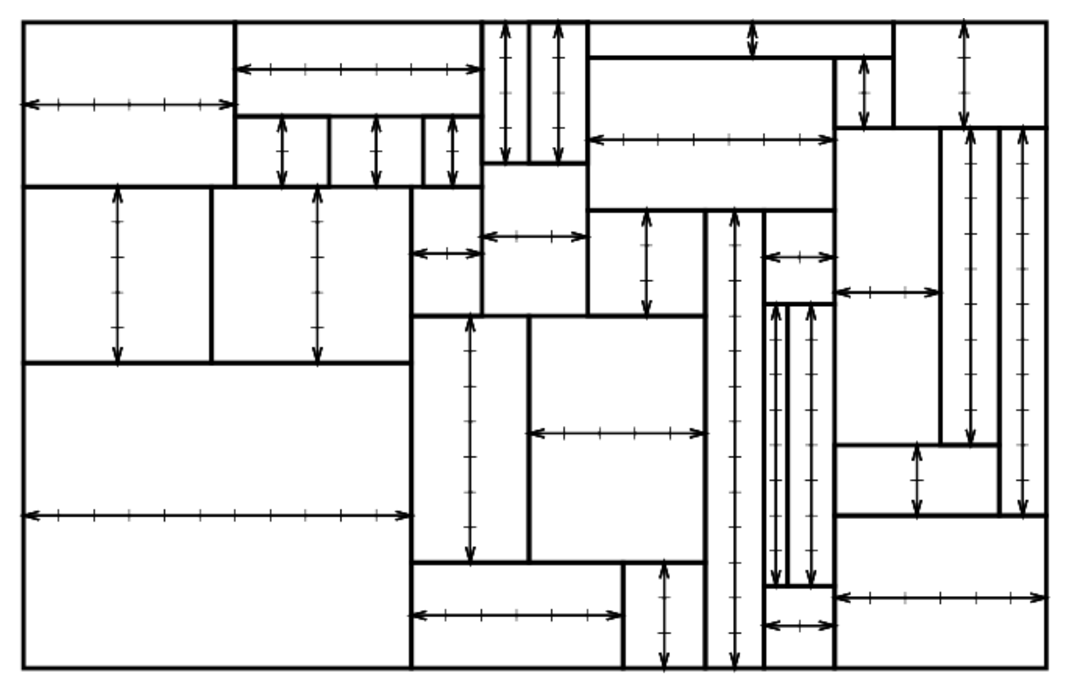
\includegraphics[scale=0.6]{Figs/Insight/rect}
\end{figure}

\subsection*{Весы и гири} %(TIPPING THE SCALES)

На столе у учителя стоят чашечные весы, правая чашка весов перевешивает.
На весах стоят гири не обязательно одного веса, на каждой из которых написаны фамилии одного \emph{или нескольких} учеников.
Ученик, входя в класс, переставляет на другую чашку весов каждую гирю, на которой написана его фамилия.
Докажите, что можно впустить в класс таких учеников, чтобы в результате перевесила левая чашка весов.

\subsection*{Часы на столе} %(WATCHERS ON THE TABLE)

На столе лежат пятьдесят точных ручных часов.
Докажите, что существует момент времени, когда сумма расстояний от центра стола до кончиков минутных стрелок больше, чем сумма расстояний от центра стола до центров часов.

\subsection*{Путь по шахматной доске} %(PATH ON CHESSBOARD)

Алиса начинает игру и ставит фишку в угол шахматной доски размером $n{\times}n$ клеток.
Боб передвигает фишку на соседнее поле, имеющее общую сторону с тем, на котором стоит фишка.
Второй раз ходить на поле, где уже побывала фишка, нельзя. 
Алиса и Боб ходят по очереди.
Проигрывает тот, кому некуда ходить.

При каких $n$ у Алисы есть выигрышная стратегия? 
При каких $n$ она выигрывает, если ее первый ход не на угловое поле, а на соседнее с ним?

\subsection*{Степень в степени} %(EXPONENT UPON EXPONENT)

На экзамене по математике для старших классов Американской школы 1960-х годов 
был следующий вопрос:
Если 
$$x^{x^{x^{{\cdot}^{\cdot^{\cdot}}}}}=2$$
Чему равен $x$? 
Предполагаемое решение основывается на том, что степень «нижнего» $x$ равна всему выражению, таким образом $x^2\z=2$ и $x=\sqrt{2}$.
Но один ученик заметил, что если бы в задаче спрашивалось решение
$$x^{x^{x^{{\cdot}^{\cdot^{\cdot}}}}}=4$$
то он бы получил тот же ответ: $x=\sqrt[4]{4}=\sqrt{2}$

Хмм...
Чему же тогда равно ${\sqrt{2}}^{{\sqrt{2}}^{{\sqrt{2}}^{{\cdot}^{\cdot^{\cdot}}}}}$? 
Можете это доказать?

\subsection*{Солдаты в поле} %(SOLDIERS IN THE FIELD)

Нечётное число солдат расположилось на поле таким образом, что все попарные расстояния между ними (между каждой парой солдат) различны.
При этом каждый солдат должен присматривать за ближайшим к нему другим солдатом.

Докажите, что существует хотя бы один солдат, за которым никто не присматривает.

\subsection*{Отрезки и расстояния} %(INTERVALS AND DISTANCES)

Пусть множество $S$ состоит из $k$ непересекающихся отрезков, лежащих в единичном отрезке $[0,1]$.
Предположим, что $S$ обладает следующим свойством: для любого вещественного числа $d$ из отрезка $[0,1]$, в множестве $S$ существуют две точки на расстоянии $d$ друг от друга.
Докажите, что сумма длин отрезков $S$ не меньше $1/k$.

 
\subsection*{Собрать 15} %(SUMMING TO 15)

Алиса и Боб по очереди выбирают число из $1, 2,\dots,9$, без повторов.
Выигрывает тот, кто первый наберет три числа, дающие в сумме 15.
Имеется ли у Алисы (она ходит первая)
выигрышная стратегия?

%ё
\section*{Решения и комментарии}

\subsubsection*{Два Биксби} % (THE BIXBY BOYS)

Классическая головоломка.
Конечно же, это были тройняшки.
Третий близнец (Арнольд?) учился в другом классе.

\subsubsection*{Свет на чердаке} % (THE ATTIC LAMP SWITCH)

Эта задача пронеслась по миру, как эпидемия гриппа, где-то лет десять тому назад; я не знаю её источника.

Действительно, невозможно определить, какой выключатель подключён к лампочке на чердаке, если всё, что у вас имеется --- это один бит информации, полученный от вашего похода на чердак.
Однако, вы можете добыть больше сведений, если используете ваши руки!
Включите выключатели 1 и 2, подождите несколько минут, затем выключите второй выключатель и идите на чердак.
Если лампочка не горит, но горячая, значит, второй выключатель это то, что мы ищем.
\heart

Если вы не можете дотянуться до лампочки, но обладаете огромным терпением, вы можете добиться того же результата, включив второй выключатель и подождав пару месяцев, затем включить первый выключатель и посетить чердак.
Если лампочка перегорела, то виноват в этом второй выключатель.

\subsubsection*{Бензиновый кризис} %(GASOLINE CRISIS)

Эта задача была известна довольно давно, вы можете найти её, например, в чудесной книге Ласло Ловаса\footnote{Laszlo Lovasz, \emph{Combinatorial Problems and Exercises}.}.
Трюк заключается в следующем:
представьте, что вы начинаете на автозаправке, скажем, №\,1 с достаточным количеством бензина и затем продолжаете свой путь, опустошая каждую автозаправку на кольцевой дороге.
Когда вы вернётесь к заправке №\,1, 
у вас будет столько же бензина, как и в начале пути.

Во время поездки записывайте, сколько бензина у вас остаётся перед каждой заправочной станцией.
Предположим, что это количество минимально перед автозаправкой №\,$k$.
Значит, если вы начнёте с автозаправки №\,$k$ с пустым баком, вы не рискуете оказаться без бензина на дороге между заправочными станциями.\heart

\subsubsection*{Бикфордовы шнуры} %(USES OF FUSES)

Подожгите одновременно оба конца первого шнура и один конец второго.
Когда первый шнур сгорит (через полминуты), подожгите незажжённый конец второго шнура.
К моменту, когда он догорит полностью, пройдёт 45 секунд.
\heart

Несколько лет назад эта и другие задачи о бикфордовых шнурах распространились по миру, как лесной пожар.
Дик Хесс, эксперт по занимательной математике, 
собрал небольшую книжку таких задач.\footnote{Dick Hess and Jerry Slocum, \emph{Shoelace Clock Puzzles}.}
Сам он впервые услышал приведённую выше задачу от Карла Морриса из Гарвардского университета.

Хесс рассматривает бикфордовые шнуры (он их зовёт шнурками) различной длины, но поджигает их только с концов.
Если же вам позволено поджигать шнур во внутренних точках и вы обладаете определённой ловкостью, то можно добиться гораздо большего.
Например, можно отмерить 10 секунд с помощью одного 60-секундного шнура, если зажечь его с обеих концов и в двух внутренних точках, а затем, каждый раз, когда сегмент сгорает, поджигать в новой внутренней точке.
Таким образом, у вас всё время горят три сегмента с двух концов, и шнур сгорает в шесть раз быстрее.

Будет немного суеты под конец и, конечно же, понадобится бесконечное число спичек, чтобы достичь абсолютной точности.

\subsubsection*{Целые числа и прямоугольники} %(INTEGERS AND RECTANGLES)}

Эта задача была предметом особой 
статьи Стэна Вэгона.%
\footnote{Stan Wagon “Fourteen proofs of a Result about Tiling a Rectangle”, American Mathematical Monthly Vol. 94, (1987) pp 601--617.}

Некоторые из решений, предложенных Вэгоном, забавным образом используют мощную математическую технику.
А одно решение не из их числа, предлагает нам следущее:
наложим на большой прямоугольник сетку, состоящую из квадратов со стороной 1/2, так, чтобы нижний левый угол прямоугольника находился в вершине клетки сетки.
Раскрасив клетки сетки в белый и чёрный цвета в шахматном порядке, 
мы видим, что каждый малый прямоугольник ровно наполовину белый и наполовину чёрный.
Следовательно, то же будет верно и для большого прямоугольника.
Но, допустим, высота большого прямоугольника не целое число, тогда часть 
большого прямоугольника между линиями $x=0$ и $x=1/2$ не содержит одинаковое количество белого и чёрного цвета.
Следовательно, основание должно быть целым числом.\heart

Автор книги несёт ответственность за следующее решение, которое вы не найдёте в статье Вэгона.
Пусть $\varepsilon$ меньше, чем наименьшая допустимая длина стороны прямоугольника разбиения.
Раскрасим каждый малый прямоугольник с целым основанием зелёным цветом, кроме красных горизонтальных полосок шириной $\varepsilon$ вдоль его верхней и нижней сторон.
Раскрасим оставшиеся прямоугольники красным, за исключением зелёных вертикальных полосок шириной $\varepsilon$ вдоль левой и правой сторон.

%в решении ссылаются на цвета диаграмы, но при печати она станет ч/б
\begin{figure}[h!]
\centering
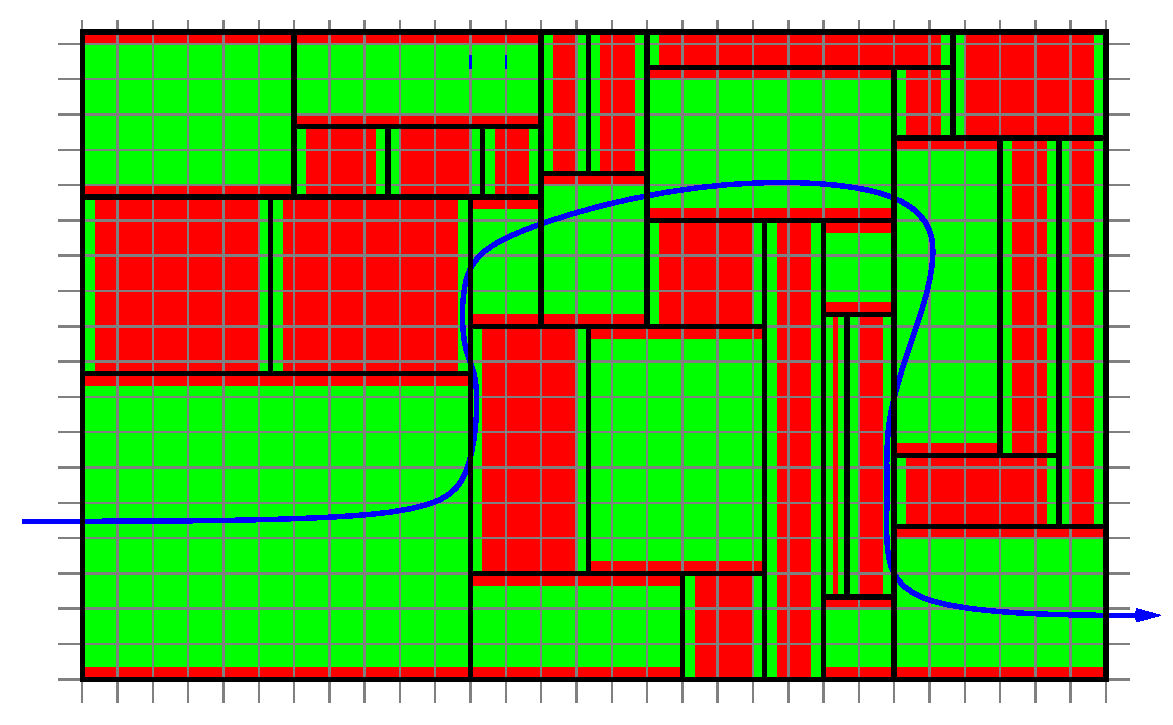
\includegraphics[scale=0.5]{Figs/Insight/green}
\end{figure}

Поместим в нижний левый угол большого прямоугольника начало координат.
Заметим, что у нас есть либо зелёный путь с левой стороны большого прямоугольника до его правой стороны, либо красный путь с нижней стороны до верхней.
Рассмотрим первый вариант.
Каждое место пересечения зелёного пути с вертикальными сторонами малых прямоугольников имеет целую координату; таким образом, основание большого прямоугольника --- целое число.
Подобным же образом и красный путь снизу вверх определяет целую высоту.

\subsubsection*{Весы и гири} %(TIPPING THE SCALES)

Рассмотрим результат для каждого подмножества учеников, включая пустое.
Заметьте, что каждая гиря окажется на левой чашке весов ровно в половине случаев.
В частности, средний вес гирь на левой чашке для всех подмножеств учеников равен их среднему весу на правой чашке.
Поскольку для пустого множества правая чашка тяжелее, 
для какого-то другого множества тяжелее должна быть левая.\heart

\noindent{\small Источник: Вторая Всесоюзная математическая олимпиада, Ленинград, 1968.}

Техника «усреднения», описанная выше, часто используется: будьте внимательны!

\subsubsection*{Часы на столе} %(WATCHERS ON THE TABLE)

Рассматривая только одни часы, 
мы видим, что в течении одного часа среднее расстояние от центра стола $C$ до кончика минутной стрелки $M$ превышает расстояние от $C$ до центра часов $W$.
Действительно, если провести через точку $C$ прямую $L$, перпендикулярную прямой $CW$, 
то среднее расстояние от прямой $L$ до точки $M$, очевидно, равно $LW$, 
что, в свою очередь, равно $CW$.
Но расстояние $CM$, по меньшей мере, равно $LM$, а обычно больше.

Взяв сумму по всем часам, приходим к аналогичному заключению, и отсюда следует, что есть момент в течении одного часа, когда желанное неравенство выполняется.\heart

\begin{figure}[h!]
\centering
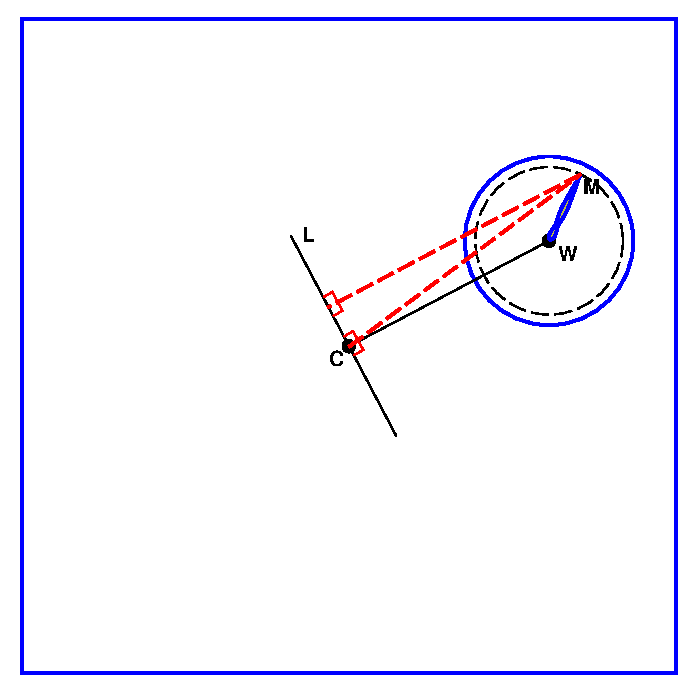
\includegraphics[scale=0.9]{Figs/Insight/watch}
\end{figure}

Требование точности часов обеспечивает движение каждой минутной стрелки с постоянной скоростью.
Это не так уж важно, когда скорости различаются, если только наше терпение не ограничено одним часом.

Одно дополнительное замечание: если установить и расположить часы определённым образом,
то \emph{можно} добиться того, что сумма расстояний от центра стола до кончиков минутных стрелок всегда была строго больше, чем сумма расстояний от центра стола до центров часов.\heart

\noindent{\smallИсточник: данная задача впервые появилась на десятой Всесоюзной математической олимпиаде в Душанбе, 1976.}

\subsubsection*{Путь по шахматной доске} %(PATH ON CHESSBOARD)

Если $n$ --- чётное число, у Боба имеется простая выигрышная стратегия, независимо от того, где Алиса начинает.
Он просто представляет себе, что шахматная доска покрыта прямоугольничками размером $1{\times2}$ клетки (домино) и каждый раз ставит фишку на вторую клетку того домино, куда пошла Алиса («закрывает» домино). %???обычно говорят «доминошки»
(Заметим, что эта стратегия работает для Боба, даже если Алисе разрешено ставить фишку на любую клетку при каждом ходе!).

Если $n$ --- нечётное, и Алиса начинает с угла, она выигрывает, если представит, что домино покрывает всю доску, кроме угловой клетки, с которой она начинает.

Tем не менее, Алиса проигрывает в случае с нечётным $n$, если она должна начинать с клетки, соседней к угловой.
Предположим, угловые клетки на данной доске чёрные, то есть Алиса начинает с белой клетки.
Существует покрытие всей шахматной доски домино, за исключением одной чёрной клетки.
Боб выигрывает, «закрывая» все домино.
Алиса
никогда не сможет поставить фишку на незакрытую клетку, потому что все клетки, на которые она ходит --- белые.\heart

\noindent{\small Источник: Двенадцатая Всесоюзная математическая олимпиада, Ташкент, 1978.}

\subsubsection*{Степень в степени} %(EXPONENT UPON EXPONENT)

Если выражение
$${\sqrt{2}}^{{\sqrt{2}}^{{\sqrt{2}}^{{\cdot}^{\cdot^{\cdot}}}}}$$
имеет какой-то смысл, то это не что иное, как предел последовательности
$${\sqrt{2}}, {\sqrt{2}}^{{\sqrt{2}}}, {\sqrt{2}}^{{\sqrt{2}}^{{\sqrt{2}}}},\dots$$
Этот предел существует, так как последовательность возрастает и ограничена.

Для доказательства первого утверждения, обозначим эту последовательность
$s_1, s_2,\dots$ и докажем по индукции, что $1<s_i\z<s_{i+1}$
для каждого $i\ge 1$.
Это сделать легко, поскольку \[s_{i+2}=
{\sqrt{2}}^{s_{i+1}}
>{\sqrt{2}}^{s_{i}}
=s_{i+1}.\]

Для нахождения верхней грани, заменим самую верхнюю степень в каждом $s_i$ на б\'{о}льшее число $2$, тогда всё выражение превращается в двойку.

Теперь, когда мы знаем, что предел существует, обозначим его $y$.
Он должен удовлетворять уравнению ${\sqrt{2}}^y=y$.
Рассмотрев уравнение $x=y^{1/y}$, 
можно увидеть, применив элементарный матанализ (приношу извинения!), 
что $x$ строго возрастает при возрастании $y$ до максимума при $y=e$
и после чего убывает.
Таким образом, существует не больше двух значений $y$, для данного $x$, 
и при $x=\sqrt{2}$ нам известны оба: $y=2$ и $y=4$.

Поскольку наша последовательность ограничена сверху двойкой, можно исключить $4$ и, таким образом, $y=2$.\heart

Обобщив приведённое выше доказательство, мы видим, что выражение $x^{x^{x^{{\cdot}^{\cdot}}}}$
имеет смысл и равно наименьшему решению уравнения $x=y^{1/y}$ при $x\le e^{1/e}$.
При $x=e^{1/e}$, выражение равно $e$ но как только $x$ превысит $e^{1/e}$, последовательность устремляется к бесконечности.

\subsubsection*{Солдаты в поле}%(SOLDIERS IN THE FIELD)

Данная задача была представлена на шестой Всероссийской математической олимпиаде в Воронеже, 1966.
Её легче всего решать, начав с двух солдат, находящихся друг от друга на кратчайшем расстоянии.
Ясно, что они присматривают друг другом, и если кто-то ещё смотрит на одного из них, тогда у нас имеется солдат, за которым присматривают дважды и, значит, есть солдат, за которым никто не присматривает.
Если же за этими двумя солдатами больше никто не присматривает, то можно их убрать, не влияя на остальных.

Так как число солдат нечётное, то, применяя и далее это рассуждение, мы, в конце концов, придём к одному солдату, который ни за кем не присматривает --- противоречие.\heart

\subsubsection*{Отрезки и расстояния} %(INTERVALS AND DISTANCES)

{\small Источник: Семнадцатая Всесоюзная математическая олимпиада, Кишинёв, 1983.}

Обозначим через $s_1,\dots,s_k$ длины отрезков множества $S$,
пусть их сумма равна $s$.
Рассмотрим интервал $I_{ij}$, содержащий все расстояния, которые можно получить, взяв первую точку на $i$-том и вторую на $j$-том отрезке множества $S$.
Ясно, что длина $I_{ij}$ равна $s_i+s_j$.
Суммируя по всем парам $i\ne j$, 
каждая длина появляется $k-1$ раз,
таким образом, сумма длин интервалов по всем парам различных отрезков, не превосходит $(k-1) s$.
Расстояния между точками, взятыми из $i$-ого отрезка, имеют значения от $0$ до $s_i$.
Значит, общая длина всех интервалов $I_{ij}$ не превосходит $k s$.
Поскольку $k s\ge 1$, получаем $s\ge 1/k$.
\heart

Равенство достигается, если максимум всех $s_i$ равен $s$, 
то есть если все отрезки, кроме одного, имеют нулевую длину.
Этого можно добиться взяв отрезок $[0,\tfrac1k]$ и добавив изолированные точки
$\tfrac2k,\tfrac3k,\dots,1$.

%исправлена фактическая ошибка --- отрезок можно брать только с краю, в середине брать нельзя.

\subsubsection*{Собрать 15} %(SUMMING TO 15)

Быстрый способ решить данную задачу --- это представить, что Алиса и Боб пользуются следующим магическим квадратом:
$$
\begin{matrix}
8&1&6\\
3&5&7\\
4&9&2
\end{matrix}
$$
Так как числа в строчке, столбике и диагонали дают в сумме 15, то можно сказать, что они играют в крестики-нолики! 
Всем известно, что наилучшая игра в крестики-нолики приводит к ничьей,
то есть ответ на наш вопрос --- нет, у Алисы нет выигрышной стратегии.
\heart

Эта забавная игра упоминается во втором томе классической книги Элвина Берлекампа, Джона Конвея и Ричарда Гая.\footnote{Winning Ways for Your Mathematical Plays by Elwyn Berlekamp, John Conway and Richard Guy ; Academic Press, 1982: 2nd Edition, A K Peters 2001}
В книге задача приписывается некоему «Э. Периколозо Спорджерси»\footnote{E. Pericoloso Sporgersi}, что выглядит очень подозрительно --- такую надпись можно увидеть в итальянских поездах, она предупреждает пассажиров об опасности высовываться из окна.

\chapter*{Числа}
\addcontentsline{toc}{chapter}{Числа}

\setlength{\epigraphwidth}{.4\textwidth}
\epigraph{Счастья светлого полны\\ %We learned to be happy,
На балу танцуем мы.\\ % We danced’ round the hall
А причину что скрывать ---\\ %And learning to count was the key to it all.
Научились мы считать.}{Граф фон Знак, «Улица Сезам»}

%The Count, “Sesame Street” 

 

Числа --- это бесконечный источник очарования, а для некоторых --- болезнь на всю жизнь. %кого-то и страсть на всю жизнь.
Бывает, что свойства конкретного числа овладевают умом человека;
про такие числа придумано множество интригующих задач,
часто требующих делать выводы из того, что на первый взгляд кажется нехваткой данных.
%основанных на кажущейся нехватке данных.

Задачи, подобранные здесь, подразумевают % предлагают 
более общий подход. % идею, более универсальный подход.
%Идея задач, подобранных здесь, --- предложить более общий, универсальный подход.
%Дух (spirit) данной коллекции ( Настроение данной коллекции подразумевает) предлагает тем не менее стремление к большей (общности )универсальности.
Наши численно-теоретические задачи о числах в целом, а не только об отдельных, особенных числах.
В ряде случаев для их решения вам понадобится несколько больше, чем знание того, 
что любое натуральное число представляется как произведение простых единственным образом.

\medskip

Вот задача для примера:

\subsection*{Двери шкафчиков}% ДВЕРИ ШКАФЧИКОВ (LOCKER DOORS)
\rindex{Двери шкафчиков}

Шкафчики в раздевалке школьного спортивного зала пронумерованы по порядку от 1 до 100.
Ученик, пришедший первым, открывает все шкафчики.
Второй ученик проходит следом и закрывает все шкафчики с чётными номерами, третий ученик меняет положение дверей у шкафчиков с номерами, кратными 3.

Так продолжается до тех пор, пока не пройдёт сотый ученик.
Какие шкафчики будут после этого открыты?
 
\paragraph{Решение:}

Состояние $n$-го шкафчика (открыт-закрыт) изменяется, когда проходит $k$-тый ученик, если $k$ --- делитель числа $n$.
Обычно, делители можно разбить на пары $\{j,k\}$, где $j\cdot k=n$.
Таким образом, совокупный эффект от учеников $j$ и $k$ на данную дверь отсутствует. %будет равен 0.
Но, если $n$ --- совершенный квадрат, то нет другого делителя, отменяющего действия $\sqrt{n}$-го ученика.
Следовательно, в конце будут открыты только шкафчики, номера которых являются совершенными квадратами: 1, 4, 9, 16, 25, 36, 49, 64, 81 и 100.\heart
 
В начале раздела мы сделаем пару наблюдений, касающихся представления целых чисел в десятичной системе счисления, и закончим неожиданно хитрой головоломкой для ужина с друзьями. % (surprisingly subtle dinner table conundrum).

\subsection*{Нули, единицы и двойки}% НУЛИ, ЕДИНИЦЫ И ДВОЙКИ. (ZEROES, ONES AND TWOS)
\rindex{Нули, единицы и двойки}

Пусть $n$ --- натуральное число.
Докажите, что (а) существует число кратное $n$ (не равное нулю), чьё представление в десятичной системе содержит только нули и единицы, и
(б) существует число кратное $2^n$, состоящее только из единиц и двоек.

\subsection*{Суммы и разности} %СУММЫ И РАЗНОСТИ (SUMS AND DIFFERENCES)
\rindex{Суммы и разности}

Даны 25 положительных чисел.
Докажите, что можно выбрать из них два числа, так, что ни одно из оставшихся чисел не равно ни их сумме, ни их разности.

\subsection*{Генерирование рациональных чисел}%??? Получение ГЕНЕРИРОВАНИЕ РАЦИОНАЛЬНЫХ ЧИСЕЛ (GENERATING THE RATIONALS)
\rindex{Генерирование рациональных чисел}

Множество $S$ содержит 0 и 1, а также средние значения всех конечных непустых подмножеств множества $S$.
Докажите, что $S$ содержит все рациональные числа единичного отрезка.

\subsection*{Суммирование дробей}%СУММИРОВАНИЕ ДРОБЕЙ ( SUMMING FRACTIONS )
\rindex{Суммирование дробей}

Дано натуральное число $n>1$, 
сложите все дроби $1/pq$, где $p$ и $q$ взаимно простые числа при $p+q>n$ и $0<p<q\le n$.
Докажите, что результат суммирования всегда равен $1/2$.

\subsection*{Вычитания по кругу}
%ВЫЧИТАЯ ПО КРУГУ (SUBTRACTING AROUND THE CORNER)
\rindex{Вычитания по кругу}

Напишите последовательность из $n$ положительных чисел.
Замените каждое из чисел на модуль разности %(absolute difference) 
этого и следующего по кругу за ним числа.
Повторяйте до тех пор, пока все числа станут равны нулю.
Докажите, что для $n=5$ этот процесс может продолжаться бесконечно, 
а при $n=4$ он всегда закачивается.

\subsection*{Прибыли и убытки}%ПРИБЫЛИ И УБЫТКИ (PROFIT AND LOSS)
\rindex{Прибыли и убытки}

На совещании акционеров правление представило помесячный отчёт о прибылях (либо об убытках) сo времени проведения последнего собрания.
«Заметьте, --- сказал генеральный директор,--- за каждые идущие подряд восемь месяцев мы получали прибыль»
«Может быть и так, --- посетовал один из акционеров, --- но я также вижу, что за каждый период из последовательно идущих пяти месяцев мы несли убытки!»

Какое максимальное число месяцев могло пройти сo времени проведения последнего собрания?

\subsection*{Первое нечётное число в словаре}%ПЕРВОЕ НЕЧЁТНОЕ ЧИСЛО В СЛОВАРЕ (FIRST ODD NUMBER IN THE DICTIONARY)
\rindex{Первое нечётное число в словаре}

Представьте, числа от 1 до $10^{10}$ записаны формальным русским языком (например, «двести одиннадцать» или «одна тысяча сорок два») и затем расставлены в алфавитном порядке (как в словаре, буква за буквой, пробелы и дефисы игнорируются).
Какое нечётное число встретится первым?

%ё
\section*{Решения и комментарии}

\subsubsection*{Нули, единицы и двойки}%НУЛИ, ЕДИНИЦЫ И ДВОЙКИ (ZEROES, ONES AND TWOS) 

Для части a) мы применим знаменитый и полезный принцип ящиков Дирихле:
Если число голубей больше числа ящиков, то хотя бы в одном из ящиков находится более одного голубя.

Мы знаем, что существует только $n$ различных остатков от деления на $n$, а множество $\{1, 11, 111, 1111,\dots\}$, чей наибольший элемент
состоит из $n+1$ цифр, содержит $n+1$ членов.
Следовательно, в нём содержатся два числа, имеющих одинаковый остаток при делении на $n$. 
Отнимите одно от другого!
\heart

Дэвид Гейл %(David Gale) 
указал мне на то, %обратил моё внимание на то, 
что если $n$ не делится на 2 и 5, то можно найти число кратное $n$, представляемое (в десятичной системе) одними единицами. 
Действительно, приведённое выше доказательство выдаёт нам число вида $111\dots111000\dots000$; 
если у нас на конце $k$ нулей, то деление на $10^k=2^k\cdot 5^k$ оставляет нам число из одних единиц и всё ещё кратное $n$. 

В части (б) легче всего, применить индукцию по $k$
и доказать, что существует число из $k$ цифр, кратное $2^k$ и состоящее только из единиц и двоек.
Добавление 1 или 2 в начало такого числа увеличит его на $2^k5^k$ или $2^{k+1}5^k$, в обоих случаях сохраняется делимость на $2^k$. 
Так как два полученных числа отличаются на $2^k5^k$, одно из них должно делится на $2^{k+1}$.
\heart

Первая задача попала ко мне от Муту Мутукришнана %(Muthu Muthukrishnan) 
из отдела исследований AT\&T и Ратгерского университета. 
Вторая была представлена на пятой Всесоюзной математической олимпиаде в Риге в 1971 году. 
Приведённое здесь решение принадлежит Саше Баргу %(Sasha Barg) 
из Мэрилендского университета.

\medskip

В похожей задаче на первой Всесоюзной математической олимпиаде в Тбилиси в 1967 году требовалось доказать, что существует число, которое делится на $5^{1000}$ и в своей десятичной записи не содержит ни одного нуля. 
Один способ --- это доказательство от противного, 
пусть $k$ --- наибольшая возможная степень пятёрки.
Пусть $n$ есть кратное наибольшей степенью пятёрки (скажем $5^j$ при $j\le k$)
среди всех $k$-значных чисел.
Тогда $n\equiv d\cdot 5^j\pmod{5^{j+1}}$ для некоторого $0<d<5$.
Отняв от $n$ число $d\cdot 10^{j+1}$ или прибавив к нему $(5-d)\cdot 10^{j+1}$
мы получим число без нулей и улучим его делимость --- противоречие.
\heart

\subsubsection*{Суммы и разности}%СУММЫ И РАЗНОСТИ (SUMS AND DIFFERENCES) 

Данная задача была также представлена на пятой Всесоюзной математической олимпиаде в Риге, 1971.

\medskip

Упорядочим числа $x_1<x_2<\dots<x_n$ (мы полагаем $n=25$ нам потребуется только, что $n$ нечётно).
Если $x_n$ не является одним из искомых чисел, значит для каждого меньшего числа $x_i$ существует другое число $x_j$, такое что $x_i+x_j=x_n$.
Таким образом первые 24 числа разбиваются на пары и значит $x_i+x_{n-i}=x_n$ для любого $i$.

Сумма $x_{n-1}$ с любым из чисел $x_2,\dots,x_{n-2}$ больше, чем $x_n=x_1+x_{n-1}$.
Значит, если $x_{n-1}$ не является одним из искомых чисел, то для каждого числа $x_i$ из $x_2,\dots,x_{n-2}$ есть пара $x_j$, что 
$x_{i}+x_{j}=x_{n-1}$.
Отсюда $x_{i}+x_{n-1-i}=x_{n-1}$ для каждого $i$.
Однако в этом случае $x_{(n-1)/2}$ парно самому себе, 
и значит пара $x_{n-1}$, $x_{(n-1)/2}$ является решением нашей задачи --- противоречие.
\heart 

\subsubsection*{Генерирование рациональных чисел}%ГЕНЕРИРОВАНИЕ РАЦИОНАЛЬНЫХ ЧИСЕЛ (GENERATING THE RATIONALS) 

В первую очередь заметим, что множество $S$ содержит все двоично-рациональные числа, 
то есть дроби вида $p/2^n$. 
Все такие числа со знаменателем $2^n$ и нечётным числителем мы можем получить, взяв среднее значение двух соседних чисел со знаменателями меньшей степени. 

Любая дробь $p/q$, очевидно, является средним $p$ единиц и $q-p$ нулей. 
Выберем $n$ достаточно большим и заменим все нули на $1/2^n$, $-1/2^n$, $2/2^n$, $-2/2^n$, $3/2^n$ и так далее, включая один $0$, если $p$ нечётное. 
Подобным же образом заменим единицы на $1-1/2^n$, $1+1/2^n$, $1-2/2^n$, $1+2/2^n$ и так далее. 
Конечно, некоторые из этих чисел находятся вне единичного отрезка, но можно повторить то же рассуждение для интервала между двоично-рациональными числами содержащего $p/q$ и лежащего строго в единичном отрезке.%(rescale the procedure to fit some dyadic interval)
\heart

Источник: Тринадцатая Всесоюзная математическая олимпиада, Тбилиси, 1979.   

\subsubsection*{Суммирование дробей}%СУММИРОВАНИЕ ДРОБЕЙ ( SUMMING FRACTIONS ) 

Проведём доказательство по индукции, заметив, что высказывание верно для $n=2$.
При переходе от $n$ к $n+1$ мы добавляем $1/pn$ для каждого $p$ с $(p,n)=1$ и теряем $1/pq$ для пар $p$ и $q$ таких, что $(p,q)=1$ и $p+q=n$.
Таким образом, каждая пара, удовлетворяющая условию задачи, означает потерю $1/pq$, и добавление $1/pn+1/qn=1/pq$, а значит результат не меняется.\heart
%(neatly cancelling).

Источник: Третья Всесоюзная математическая олимпиада, Киев, 1969. 

\subsubsection*{Вычитания по кругу}%ВЫЧИТАЯ ПО КРУГУ (SUBTRACTING AROUND THE CORNER) 

Один внештатный преподаватель математики старших классов (средняя школа в Фер Лон, Нью-Джерси, 1962)
%(Fair Lawn Senior High School) 
рассказывал мне,
что некоторые военнопленные Второй Мировой войны развлекались тем, что брали различные наборы из четырёх чисел и смотрели как долго они могут прокручивать эту операцию. 

\medskip

Обе задачи решаются рассмотрением процесса по модулю 2.
Для $n=4$ с точностью до циклических перестановок и симметрий, 1 0 0 0 и
1 1 1 0 становятся 1 1 0 0, затем 1 0 1 0, затем 1 1 1 1 и затем 0 0 0 0.
Поскольку здесь охватываются все случаи, мы видим, что при работе с обычными целыми числами нам понадобится не более 4 шагов, чтобы все они стали чётными, и на этом этапе, до того, как продолжить далее, мы можем поделить их на двойку в наибольшей общей степени. 
Так как самое большое в последовательности число $M$ не может увеличиваться и уменьшается в два раза или более хотя бы один раз за каждые четыре шага, 
мы приходим к 0 0 0 0 максимум за $4(1+\lceil\log_2 M\rceil)$ шагов.

С другой стороны, при $n=5$ последовательность 1 1 0 0 0 (рассматриваемая как последовательност бинарных или обычных чисел)
проходит по циклу 
1 0 1 0 0, 
1 1 1 1 0, 
1 1 0 0 0.\heart 

Несложный анализ, использующий многочлены над целыми по модулю два, показывает, что всё зависит от того является ли $n$ степенью двойки. 

\subsubsection*{Прибыли и убытки}%ПРИБЫЛИ И УБЫТКИ (PROFIT AND LOSS) 

Данная задача представляет собой адаптированный вариант задачи, предложенной одним вьетнамским автором на Международной Математической Олимпиаде 1977 года. 
Мне её рассказал Титу Андрееску, %(Titu Andreescu), 
за что я ему очень благодарен. 
Решение, однако, моё собственное. 

Нам нужна, конечно, последовательность чисел максимальной длины, такая, что сумма чисел каждой подстроки длины 8 --- больше нуля, а сумма чисел каждой подстроки длины 5 --- меньше нуля. Строка, без сомнения, должна быть конечной, более того, длиной меньше 40, иначе вы могли бы выразить сумму первых 40-ка членов и как (положительную) сумму 5 подстрок длины 8, и как сумму (отрицательную) 8 подстрок длины 5.  

Давайте решим эту задачу в более общем виде. Пусть $f(x,y)$ --- длина максимальной строки, такой, что сумма каждой $x$-подстроки положительна, а сумма каждой $y$-подстроки --- отрицательна. 
Мы можем предположить, что $x>y$. 
Если $x$ кратно $y$, тогда $f(x,y)=x-1$ --- мы должны согласиться, что это утверждение верно по отношению к $x$-подстрокам за отсутствием таковых. 

Что, если $y=2$ и $x$ --- нечётное?
Тогда можно построить строку длины $x$ с чередующимся элементами, скажем, $x-1$ и $-x$. 
Однако такой строки длины $x+1$ не существует.
Действительно, в каждой $x$-подстроке нечётный элемент должен быть положительным 
(так как можно покрыть всю $x$-подстроку 2-подстроками за исключением произвольного нечётного элемента). 
Для двух $x$-подстрок, это означает, что все элементы положительны ---
противоречие.  

Рассуждение выше подсказывает, что $f(x,y)\le x+y-2$, если $x$ и $y$ взаимно просты, 
то есть не имеют общего делителя отличного от~1. 
Докажем это по индукции. 
Рассуждая от противного, предположим что $f(x,y)\ge x+y-1$;
то есть имеется строка длины $x+y-1$, удовлетворяющая указанным условиям. 
Положим $x=ay+b$, где $0<b<y$. 
Заметим, что каждая $b$-подстрока %(any consecutive b of them) 
может быть представлена как $x$-подстрока полной строки, 
без $a$ штук $y$-подстрок; 
следовательно, сумма в любой $b$-подстроке положительна. 
Отсюда
$f(b,y)\ge x+y-1$,
что противоречит предположению индукции поскольку $y$ и $b$ взаимно просты и $b<y<x$.

Чтобы показать, что $f(x,y)=x+y-2$, когда $x$ и $y$ взаимно просты, мы построим $(x+y-2)$-строку, обладающую требуемыми свойствами.
Более того, числа нашей строки будут принимать ровно два различных значения $u$ и $v$,
а также строка будет периодической с двумя периодами $x$ и $y$. 

Представим себе, что мы расставили $u$ и $v$ их произвольным образом в первой $y$-подстроке.
Продолжим расстановку, заставляя строку быть периодической с периодом $y$.
Чтобы добиться того же с периодом $x$,
нам нужно обеспечить, чтобы последние $y-2$ элементов соответствовали первым.
Это условие можно записать как $y-2$ равенств на $y$ значений выбранных нами изначально. 
Поскольку этих равенств недостаточно, чтобы заставить все решения быть одинаковыми, мы можем гарантировать, что существует по меньшей мере одно $u$ и одно $v$.

Проделаем это для $x=8$ и $y=5$.
Пусть $c_1\dots c_5$ будут первые пять элементов строки, 
таким образом вся строка будет выглядеть как
$c_1c_2c_3c_4c_5c_1c_2c_3c_4c_5c_1$. 
Для того, чтобы строка была периодична с периодом 8, 
нужно потребовать $c_4=c_1$, $c_5=c_2$ и $c_1=c_3$. 
Значит можно считать $c_1=c_3=c_4=u$ и $c_2=c_5=v$; 
тем самым получается последовательность $uvuuvuvuuvu$. 

Возвращаясь к задаче в общем виде, 
заметим, что строка с периодом $x$ автоматически обладает следующим свойством: сумма каждой $x$-подстроки одна и та же, потому как, каждый раз, когда вы сдвигаете $x$-подстроку на один шаг, элемент, приобретённый на одном конце, такой же, как и элемент, потерянный на другом.
Конечно, это высказывание справедливо и для $y$-подстрок, если строка периодична с периодом $y$.

Пусть $S_x$ --- сумма $x$-подстроки, a $S_y$ --- сумма $y$-подстроки. 
Заметим, что $S_x/x\ne S_y/y$.
Это объясняется тем, что, если у нас $u$ встречается в каждой
 $x$-подстроке, скажем, $p$ раз, а $v$, в каждой $y$-подстроке --- $q$ раз, 
 то равенство $S_x/x=S_y/y$
 означало бы 
\[y(pu+(x-p)v)=x(qu+(y-q)v)\]
что сводится к $yp=xq$ так как $u\ne v$. 
Поскольку $x$ и $y$ взаимно простые, этого не может быть при $0<p<x$ и $0<q<y$. 

Отсюда следует, что можно подобрать $u$ и $v$ так, чтобы сумма $S_x$ была положительна, а $S_y$ отрицательна. 
Например, в случае, рассматриваемом выше, каждая 8-подстрока содержит пять $u$ и три $v$, 
а в свою очередь, каждая 5-подстрока имеет три $u$ и две $v$.
Если взять $u=5$ и $v=-8$, то получим $S_x=1$ и $S_y=-1$. 
Итак, решением исходной задачи будет последовательность $5,-8,5,5,-8,5,-8,5,5,-8,5$.
\heart

Усердный читатель легко обобщит вышеприведённое доказательство на случай, 
когда наибольший общий делитель $x$ и $y$ отличнен от~1. 
Результат будет $f(x,y)=x+y-1-\text{НОД}(x,y)$.    

\subsubsection*{Первое нечётное число в словаре}%ПЕРВОЕ НЕЧЁТНОЕ ЧИСЛО В СЛОВАРЕ (FIRST ODD NUMBER IN THE DICTIONARY) 

Решение данной задачи --- всего лишь вопрос внимательного и методичного рассмотрения последовательности слов, составляющих числительные.
Самое первое число будет, конечно, «восемнадцать», и первое идущее за ним слово (можем считать его как бы суффиксом) --- «миллионов».
Итак, искомое число должно начинаться с «восемнадцать миллионов», следуя подобным образом далее, мы получаем окончательный ответ какой 18 018 089 --- «восемнадцать миллионов восемнадцать тысяч восемьдесят девять».%
\footnote{Ответ в оригинальной задаче на английском языке выглядит похоже: 8,018,018,885 --- «eight billion eighteen million eighteen thousand eight hundred eighty-five».}
\heart

Идея этой забавной задачи пришла ко мне после того, как Херб Уилф из Пенсильванского университета %(Herb Wilf, University of Pennsylvania) 
попросил меня назвать первое простое число в словаре. 
Автором этого вопроса считается компьютерный гуру из Стэндфордского университета Дональд Кнут. %(Donald Knuth, Stanford University).
Рассуждая так же как и выше, с проверкой простоты числа на компьютере
получаем, что ответ равен 18 018 881.%
\footnote{На английском, это будет 8,018,018,881 --- «eight billion eighteen million eighteen thousand eight hundred eighty-one».}


\chapter*{Комбинаторика}
\addcontentsline{toc}{chapter}{Комбинаторика}

\setlength{\epigraphwidth}{.6\textwidth}
\epigraph{Ложь имеет бесконечное число комбинаций,
тогда как правда бывает только одна.}{Жан-Жак Руссо}

 
 
Если задача начинается со слов «Сколько существует способов...», то это автоматически задача по комбинаторике, но обратное неверно.
Комбинаторный подход будет полезен при решении как нижеследующих (довольно разнообразных) задач, так и многих других в этой книге.

Наша вводная задача совершенно классическая и использует фундаментальную
комбинаторную технику --- перемножение чисел независимых вариантов.

\subsection*{Расстановка цифр}% (Sequencing the Digits)
\rindex{Расстановка цифр}

Сколькими способами можно записать в ряд цифры от 0 до 9, так, что каждая цифра, кроме самой левой, отличается от одной из цифр стоящих слева от неё, на единицу.

\paragraph{Решение:} На первый взгляд кажется, что данная задача не решается перемноженим чисел независимых вариантов, так как число вариантов зависит от предыдущего выбора.
Например, у нас есть десять вариантов для самой левой цифры,
но начав ряд, скажем, с «3» у нас только два варианта для следующей цифры; если же мы начинаем с «0» или «9», то у нас только один выбор.
Если вы знаете как суммировать биномиальные коэффициенты, то вы можете построить на этом решение задачи, но есть лучший способ.

Заметим, что ряд заканчивается нулём или девяткой; и если мы движемся \emph{справа налево}, то каждый раз мы стоим перед выбором --- написать наибольшую неиспользованную цифру или наименьшую, пока не дойдём до левого края, где эти два выбора совпадают.
Таким образом, получаем два выбора в каждой из девяти возможностей.
Отсюда ответ $2^9=512$ способов.\heart

(Источник: Олимпиада Патнема 1960-х годов.)% (A Putman Exam from the 1960s )

\bigskip

За вами решение оставшихся задач.
Подсказка: смотрите внимательно, где можно применить принцип Дирихле!

\subsection*{Подмножества подмножеств}% (Subsets of subsets)
\rindex{Подмножества подмножеств}

Докажите, что любое множество из десяти различных чисел от 1 до 100 содержит два непересекающихся непустых подмножества, сумма чисел которых одинакова.

\subsection*{Вредный метрдотель}% (The Malicious Maitr D’)
\rindex{Вредный метрдотель}

На банкете математической конференции 48-ми мужчинам математикам, ни один из которых не имеет ни малейшего представления об этикете, назначены места за большим круглым столом.
На столе, между каждой парой приборов, стоит кофейная чашка с салфеткой.
Как только человек занимает своё место (по указанию метрдотеля), он берёт салфетку, слева или справа от себя; если на столе две салфетки, он выбирает одну случайным образом (но метрдотель не может видеть, какую).

В каком порядке следует заполнять места, чтобы максимальному числу математиков не досталось салфетки?

\subsection*{Рукопожатия на приёме}% (Handshakes at a Party)
\rindex{Рукопожатия на приёме}

Майк и Жанна, а также ещё четыре пары, побывали на праздничном обеде, где каждый из присутствующих обменялся рукопожатием с каждым, ему дотоле незнакомым гостем.
Позже Майк опросил всех и обнаружил, что каждый из девяти других гостей пожал руки с \emph{разным} числом людей.

Со сколькими гостями обменялась рукопожатиями Жанна?

\subsection*{Трёхсторонние выборы}% (Three-Way Election)
\rindex{Трёхсторонние выборы}

Ашворд, Бакстер и Кэмпбелл баллотируются на пост председателя союза %(secretary of union) 
и набирают по одинаковому числу голосов.
Для разрешения этой ситуации они требуют голосования с учётом второго выбора избирателей (так называемого преференциального метода голосования), но снова приходят к ничьей.
Тогда Ашворд выступает с предложением, что, так как число избирателей нечётное, можно провести двухсторонние выборы --- избиратели выбирают между Бакстером и Кэмпбеллом, а затем между победителем и Ашвордом.

Но Бакстер недоволен данным предложением.
Он считает этот способ несправедливым, потому что, по его мнению, у Ашворда больше шансов выиграть, чем у остальных.
Прав ли Бакстер?

\subsection*{Зарплата короля}% (King’s Salary)
\rindex{Зарплата короля}

После революции каждый из 66 жителей некой страны, включая короля, получает зарплату в 1 доллар.
Король не может больше голосовать, но всё ещё сохраняет за собой право вносить изменения в законопроект, в частности, в то, как распределяется зарплата.
Зарплата каждого жителя должна быть целым числом долларов и сумма всех зарплат равняется 66.
Каждое предложение по изменению ставится на голосование и принимается, если получает больше голосов «За», чем «Против».
Будем считать, что те, кто получают прибавку к зарплате, голосуют «За», а те, у кого зарплата уменьшается --- «Против», остальные же голосованием себя не утруждают.

Король --- человек умный и корыстный.
Какой максимальной для себя зарплаты он может добиться, и сколько шагов ему на это понадобится?

\subsection*{Плохо сделанные часы}% (A Poorly Designed Clock)
\rindex{Плохо сделанные часы}

Есть часы, у которых минутная стрелка никак не отличается от часовой.
Сколько раз в сутки возникнет ситуация, когда по этим часам нельзя определить время в данный момент?

\subsection*{Таинственный карточный фокус}% (A Mystifying Card Trick )
\rindex{Таинственный карточный фокус}

Давид и Дороти придумали хитрый карточный фокус.
Давид отворачивается, кто-нибудь выбирает пять карт из колоды карт для бриджа и даёт их Дороти; она просматривает карты, вытаскивает одну и передаёт оставшиеся карты Давиду.
Давид правильно называет вытащенную Дороти карту.

Как они это делают?
На какой наибольшей колоде возможно демонстрировать их фокус?

\subsection*{Странствующие торговцы}% (Travelling Salesmen )
\rindex{Странствующие торговцы}

Между любыми двумя большими городами в России цена авиабилетов фиксирована.
Алексей Фругаль, коммивояжёр, начинает свою поездку по городам из Москвы и всегда выбирает самый дешёвый перелёт до города, который он ещё не посещал.
(Ему не нужно каждый раз возвращаться в Москву).
Коммивояжёру Борису Лавишу также нужно посетить каждый город, но он начинает свою поездку в Калининграде и каждый раз выбирает самый дорогостоящий перелёт до города, в котором он ещё не побывал.

Докажите, что поездки Лавиша стоят как минимум столько же, сколько поездки Фругаля. %???Фругаль = Скряга, Лавиш=Кутила

\subsection*{Проигрыш в кости}% (Losing at Dice)
\rindex{Проигрыш в кости}

При броске шести кубиков, число различных выпавших чисел варируется от 1 до 6.
Предположим, что каждую минуту крупье бросает шесть кубиков,
и вы ставите 1 доллар, один к одному, на то, что выпадет ровно 4 различных числа
(то есть вы получаете 1 доллар, если выигрываете или теряете 1 доллар, если проигрываете).

Если вы начинаете игру с 10 долларами, приблизительно, сколько вы в среднем продержитесь до полного проигрыша?

\section*{Решения и комментарии}

\subsubsection*{Подмножества подмножеств}% (Subsets of subsets)

Хитрость в данной задаче, основанной на одном из заданий Международной математической олимпиады 1972 года, заключается в том, что вначале условие непересечения подмножеств игнорируется, и рассматриваются все подмножества.

\medskip

Множество $S$ из $10$ элементов содержит, разумеется, $2^{10} - 1 \z= 1023$ непустых подмножества.
Могут ли все суммы чисел этих подмножеств быть различными?
Максимальная сумма подмножества множества из десяти чисел от 1 до 100 будет 
$100+99+\dots+91\z<1000$, а минимальная, очевидно, равна 1; таким образом, согласно принципу Дирихле, должны существовать два различных подмножества $A\subset S$ и $B\subset S$ 
с одинаковой суммой.
Конечно, $A$ и $B$ могут пересекаться, но можно просто выбросить общие элементы;
$A\backslash B$ (множество элементов $A$, не содержащихся в $B$) и $B\backslash A$ \emph{не} пересекаются и по-прежнему имеют одинаковую сумму.\heart

\subsubsection*{Вредный метрдотель}% (The Malicious Maitr D’)

Появление данной задачи связано со следующим событием:
30 марта 2001 года принстонский математик Джон Хортон Конвей %(John H. Conway) 
прибыл года в лаборатории Белла, %(Bell Labs) 
чтобы сделать доклад на «Общенаучном семинаре». %(“General Research Colloquium”).
На обеде ваш автор оказался сидящим за столом между Конвейем и специалистом по компьютерным технологиям Робом Пайком %(Rob Pike) 
(сейчас работает в Гугле), и салфетки, и кофейные чашки были расставлены точно так же, как описано в задаче.
Конвей задался вопросом, а сколько человек из
сидящих за столом остались бы без салфеток, если бы их рассаживали в \emph{случайном} порядке (см. Главу 11), а Пайк сказал: «А вот более лёгкий вариант: а какой порядок \emph{самый плохой}?»

\bigskip

Допустим, что метрдотель, когда сажает человека на место, видит, которую салфетку взяли (такого игрока называют «адаптивным противником»). %(“adaptive adversary”) 
Тогда лучшая для него стратегия состоит в следующем:
если первый гость возьмёт салфетку, скажем, справа от себя, то следующий будет посажен на второе место справа, так что тот, кто окажется между ними, может попасть в западню.
Если второй человек берёт салфетку справа, то метрдотель пытается делать то же самое и дальше, пропуская одно место справа.
Если же второй человек возьмёт салфетку слева (оставляя, таким образом, место между ним и первым посаженным без салфеток), то третий сажается сразу справа от второго.
Далее гостям указываются места соответственно этому правилу, пока круг не замкнётся, и тогда последние обедающие (обречённые остаться без салфеток) садятся за стол.
В результате в среднем, $1/6$ часть гостей остаётся без салфеток.

Когда же, как в поставленной задаче, метрдотель не «адаптивный противник», то, как показалось Пайку и мне, правильной стратегией было бы заполнить сначала все чётные, а затем нечётные места.
Для каждого нечётного гостя вероятность остаться без салфетки будет равна $1/4$, %(for an overall yield) 
а конечным результатом будет $1/8$ (то есть 6 из 48 обедающих, в среднем).

Хотя, если подумать ещё немного, то наилучшая стратегия для метрдотеля --- заполнить сначала места с номерами $0\pmod4$, затем нечётные места, и, наконец места $2\pmod4$.
Это расстроит $9/64$ гостей, в среднем.
Чтобы понять это, назовём гостя «одиноким», если, когда он посажен на место, у него ещё нет соседа ни справа, ни слева.
Можно предположить, что все «одинокие» гости рассаживаются первыми, и заметим, что между каждой сидящей подряд парой «одиноких» будет максимум один бессалфеточный гость.

Допустим, два последовательно сидящих «одиноких» гостя находятся на расстоянии $d$ друг от друга (то есть между ними $d-1$ стульев).
Эти места будут заполняться с обеих сторон.
Предположим, последний садящийся между ними человек находится на расстоянии $a$ от правого и на расстоянии $b$ от левого «одинокого» гостя, где $a+b=d$.
Правая салфетка будет уже взята, если только «одинокий» обедающий не сидит сразу справа от него, и все последующие гости между парой «одиноких» не выбрали левые салфетки.
Это случается с вероятностью $1/2^a$.
Таким образом, оказавшийся в ловушке 
гость проигрывает (остаётся без салфетки) с вероятностью
\[(1-2^{-a})(1-2^{-b})=1 + 2^{-d}-2^{-a}-2^{-b},\]
которая минимальна, когда $a$ и $b$ равны или отличаются на 1.

Если «одинокие» гости рассажены на расстоянии $d$ друг от друга, то мы получаем одного потенциального проигравшего на $d$ человек.
Таким образом, если число гостей $n$ кратно $d$, то среднее число проигравших равно $(n/d)(1-2^{-\lfloor d/2\rfloor})(1-2^{-\lceil d/2\rceil})$.
Легко проверить, что эта величина достигает максимума не при $d=2$, где она будет равна $n/8$, а при $d=4$, где получаем $9n/64$.
\heart

\subsubsection*{Рукопожатия на приёме}% (Handshakes at a Party)

Данная задача на старую избитую тему --- на первый взгляд, нам кажется что предоставлено недостаточно информации.
С чего, казалось бы, можно сказать что-то о \emph{Жанне}?
Ответом, в конечном итоге, окажется то, что Жанна в паре с тем, кто не принимал участия в опросе.

Так как для каждого гостя максимальное число рукопожатий будет равно 8, 
девять ответов, полученных Майком, --- это как раз числа от 0 до 8.
Два человека (скажем, $A$ и $B$), ответившие 0 и 8, должны быть парой, ведь в противном случае наличие и отсутствие рукопожатия между ними противоречило бы одному из их ответов.
Теперь проверим $C$ и $D$, которым соответствуют 1 и 7;
поскольку $C$ должен был пожать руки с $B$, а $D$ должен был пропустить $A$, то, применяя рассуждение выше, получаем, что $C$ и $D$ так же являются парой.

Аналогично, гости, ответившие 2 и 6, 3 и 5 также должны быть парами.
Значит Майк и Жанна пожали руки гостям, с б\'{о}льшим результатом опроса;
то есть, каждый из них пожал руку четырём.
\heart

Если вы не нашли доказательства, но догадались, что ответ~4, то ваша интуиция была права.
Если предположить что задача имеет единственный ответ (скажем $x$), то в силу симметрии $x=4$.
Предположим, что (по какой-то причине) каждая пара пожала руки друг-другу, и Майк спросил каждого скольким гостям тот \emph{не} пожал руку.
Тогда Женни должна была пожать $x+1$ рук.
Но смена местами роль рукопожатий и нерукопожатий влечёт, что $x+(x+1)=9$.

Тот факт, что головоломка имеет единственное решение часто оказывается полезным.
В одной из своих «Математических игр» для \emph{Scientific American}, Мартин Гарднер спросил:
Предположим дырка длиной в 6 дюймов просверлена через центр шара, чему равен оставшийся объём?

Может показаться, что для решения задачи необходимо знать диаметр дырки, или диаметр исходного шара, но на самом деле этого не нужно.
Чем больше шар тем шире должна быть дырка, для того чтобы иметь длину 6 дюймов;
при этом вычисления показывают, что объём оставшегося кольца не меняется.

Однако нет необходимости делать эти вычисления если поверить, что решение единственно.
Ответ должен быть то же для шара с 6 дюймами в диаметре и без дырки, а именно $\tfrac43\pi3^3=36\pi$ кубических дюймов.

\subsubsection*{Трёхсторонние выборы}% (Three-Way Election)

Бакстер прав, более того, он недооценивает ситуацию.
Представим себе, что никто из голосующих не изменяет своего выбора, тогда несомненно выигрывает Ашворд!
Предположим, что избиратели, голосовавшие за Ашворда, предпочитают Бакстера Кэмпбеллу (то есть Бакстер выиграет у Кэмпбелла в предложенных двухсторонних выборах).
Тогда избиратели, голосовавшие за Бакстера, должны предпочитать
Кэмпбелла Ашворду, иначе Кэмпбелл не набрал бы $1/3$ голосов второго выбора.
Аналогично, избиратели, голосовавшие за Кэмпбелла, предпочитают Ашворда
Бакстеру.
Таким образом, в нашем случае, Ашворд побеждает Бакстера во втором
голосовании.

Если же избиратели, голосовавшие за Ашворда, предпочитают Кэмпбелла Бакстеру, то симметричное рассуждение приводит нас к тому же результату --- во втором голосовании побеждает Ашворд.
\heart

Эта задача, придумана Эхудом Фридгутом %(Ehud Friedgut)
для работы в классе;
она указывает на то, что разрешение ничьи не так уж просто, как кажется на первый взгляд!

\subsubsection*{Зарплата короля}% (King’s Salary)

Данная задача придумана Йоханом Вестлундом %(Johan Waestlund) 
из Линчёпингского университета, а идея её была навеяна историческими событиями в Швеции.
Тут нужно сделать два важных замечания: (1) король должен временно отдать свою зарплату, чтобы начать эту игру, и (2) на каждом шаге следует уменьшать число жителей, получающих зарплату.

Король начинает с того, что предлагает удвоить зарплату $33$ жителям (они получат по $2$ доллара) за счёт остальных $33$ граждан, включая его самого.
Затем, он увеличивает зарплату $17$ из $33$ оплачиваемых жителей (они получат по $3$ или $4$ доллара), а оставшиеся $16$ останутся в нулях.
На каждом последующем шаге число голосующих граждан сводится к $9$, $5$, $3$ и $2$.
В конце концов, король подкупает $3$ бедняков зарплатой в $1$ доллар каждому, для того, чтобы они помогли ему перевести две большие зарплаты на него самого, и, таким образом, завершает игру с королевской зарплатой в $63$ доллара.

Нетрудно заметить, что на каждом этапе король не может предпринять ничего лучшего, чем уменьшать число людей с зарплатой до чуть больше половины.
В частности, он не сможет оставить с зарплатой только одного человека.
Стало быть, $63$ доллара --- это лучшее, чего он сможет добиться, и оптимальное число шагов равно $6$.
\heart

В более общем случае, если начальное число жителей равно $n$, король может добиться зарплаты в $n-3$ доллара за $k$ шагов, где $k$ --- наименьшее целое число большее или равное $\log_2(n-2)$.

\subsubsection*{Плохо сделанные часы}% (A Poorly Designed Clock)

Энди Латто %(Andy Latto, 
(andy.latto@pobox.com) инженер-программист из Бостона, представил эту прелестную задачу в Атланте, на конференции «Gathering for Gard\-ner IV», одной из серии конференций в честь Мартина Гарднера.
При достаточном терпении и внимательности задачу можно решить алгебраическим или геометрическим способом, но есть замечательное доказательство без карандаша и бумаги, предложенное Майклом Ларсеном, %(Michael Larsen)
профессором математики из университета Индианы.
Идею третьей стрелки (вместо вторых часов) подсказал Дэвид Гейл. %(David Gale)

\medskip

Для начала отметим, для того, чтобы эта задача имела какой-либо смысл, нам надо предположить, что стрелки движутся непрерывно, и что мы не заботимся о том, утро это или вечер.
Обратим также внимание, что можно сказать, сколько времени, когда стрелки совпадают, даже если мы не знаем, какая стрелка какая.
Это случается $22$ раза в день, так как за день минутная стрелка делает полный оборот $24$ раза, а часовая --- $2$ раза, в том же направлении.

Это наблюдение послужит нам в дальнейшем доказательстве.
Представим, что мы добавляем к нашим часам третью, «быструю» стрелку, которая начинает ходить в $12$ часов полуночи и ровно в $12$ раз быстрее, чем минутная стрелка.

Итак, будем говорить, что каждый раз, когда часовая и быстрая стрелка совпадают, они находятся в неопределённом положении.
Почему?
Потому что позже, когда минутная стрелка пройдёт в $12$ раз больше, она окажется там, где быстрая стрелка (а, следовательно, и часовая) находятся в данный момент.
По тем же соображениям верно и обратное утверждение: все неопределённые положения случаются тогда, когда часовая и быстрая стрелка совпадают.

Нам остаётся только вычислить, сколько таких совпадений происходит за один день.
Быстрая стрелка делает $12^2\times 2 = 288$ оборотов в день, а часовая только два, таким образом, случается 286 совпадений.
Из них 22 раза совпадают минутная и часовая стрелки (то есть все $3$ стрелки), оставляя 264 неопределённых моментов. 
\heart

\subsubsection*{Таинственный карточный фокус}% (A Mystifying Card Trick ) 

Данный карточный фокус обычно приписывается математику Уильяму Фитч Чейни. % (William Fitch Cheney).
Более подробную информацию читатели могут найти в статье Майкла Клебера\footnote{M. Kleber, ``The best card trick''. \emph{Math. Intell.} 24.1 (2002): 9--11.};
или в статье Колма Малкэхи%
\footnote{C. Mulcahy, ``Fitch Cheney's five card trick''. \emph{Math Horizons} 10.3 (2003): 10--13.}, в которой обсуждаются различные варианты этого фокуса.

\medskip

Итак, Дороти сообщает Давиду информацию только через порядок четырёх карт, которые она ему передаёт.
Конечно, у нас только $4!=24$ возможных перестановок на $48$ вариантов для пятой карты, хитрость в том, что Дороти ещё решает, какую из пяти карт выбрать.

Самый простой способ для Дороти, который я знаю, --- это выбрать карту той масти, которая представлена хотя бы дважды (опять принцип Дирихле!).
Предположим, что это пики, обозначим карты $x$ и $y$ (будем думать о них как о числах между Тузом $=1$ и Королём $=13$, по модулю 13).
В одну сторону или в другую карты отстоят друг от друга не более чем на 6;
допустим, что $x$ «больше», так что $x-y\in {1,2,3,4,5,6} \pmod{13}$.
Таким образом, например, у нас может быть $x =3\equiv 16$ и $y = 12$ (Дама пик), так что $x-y\equiv4$.

Дороти выбирает $x$, ставит $y$ первой из оставшихся четырёх карт и тремя другими картами кодирует разность $x-y$.
Например, представим, что Дороти и Давид договорились о следующем порядке колоды: 
$\clubsuit\text{Т},
\clubsuit 2,
\dots
\clubsuit\text{К},
\Diamond\text{Т},
\dots,
\Diamond\text{К},
\heartsuit\text{Т},
\dots,
\heartsuit\text{К},
\spadesuit \text{Т},
\dots,
\spadesuit \text{К}$.
Если карты стоят по возрастанию (скажем, 
$\clubsuit 5,
\clubsuit \text{В},
\Diamond 3$), то $x-y\z=1$; обозначим этот порядок $123$.
Положим $x-y=2$ для порядка $132$,
$x-y=3$ для $213$, $x-y=4$ для $231$, $x-y=5$ для $312$ и, наконец, $x-y=6$ для $321$.

Конечно, придётся немного потренироваться, чтобы показывать этот фокус безупречно.

\medskip

Обратите внимание на слабое место в этой схеме: если среди пяти карт, полученных Дороти, мастей представлено меньше четырёх, то она имеет, по меньшей мере, два варианта выбора карты.
Естественно будет задаться вопросом: насколько больше может быть колода карт, чтобы всё ещё можно было исполнить фокус;
максимум оказывается равным $124$.

Покажем, что лучше сделать невозможно.
Представим, что карты пронумерованы от $1$ до $n$ и рассмотрим функцию $f$, которая каждой упорядоченной четвёрке $(u,v,y,z)$ с попарно различными элементами сопоставляет пятую карту $x$, ту, которую Давид должен определить, глядя на эту четвёрку.
Чтобы фокус получился, Дороти должна уметь, имея
любое множество $S$ из пяти элементов в ${1, \dots, n}$, выбрать четыре элемента $(u,v,y,z)$ так, что $S = \{u,v,y,z, f(u,v,y,z)\}$.
Таким образом, число всех четвёрок должно быть, по меньшей мере, равно числу всех множеств из пяти элементов, то есть
\[n(n - 1)(n - 2)(n - 3)\ge \binom n5,\]
что влечёт $n - 4 \le5!$ и, значит, $n\le 124$.


Исполнить фокус с картами, пронумерованными от $1$ до $124$, удивительно легко.
Вот способ, предложенный Элвином Берлекэмпом.
%(Elwyn Berlekamp).
Допустим, выбранные карты $c_1 < c_2 < \dots < c_5$;
Дороти берёт карту $c_j$, где $j$ --- сумма значений всех пяти карт по модулю 5.
Глядя на оставшиеся четыре карты, сумма которых равна, скажем, $s$ по модулю 5, Давид должен найти число $x$ такое, что $x\equiv -s + k \pmod 5$, если $x$ есть $c_k$.

Другими словами, либо $x$ --- меньше, чем любая из карт Давида и удовлетворяет 
$x\equiv-s + 1 \pmod 5$; либо $x$ больше наименьшей карты, но меньше следующей за ней, и 
$x\equiv -s + 2 \pmod 5$; и так далее.
Но это всё равно, что сказать, что $x\equiv -s + 1 \pmod 5$,
\emph{если оставшиеся $120$ карт перенумерованы подряд от 1 до 120},
пропуская четыре карты в руках у Давида.

Ровно $120/5 = 24 = 4!$ чисел от 1 до 120 имеют данное значение по модулю 5.
Поэтому, переставляя четыре карты Давида, можно закодировать все возможные значения $x$.
\heart

\subsubsection*{Странствующие торговцы} %(Travelling Salesmen )

Данная задача, представленная на 11-й Всесоюзной математической олимпиаде в Таллине в 1977 году, досадно трудна. %(annoyingly tricky) 
\emph{Очевидно}, что Лавиш тратит, по меньшей мере, столько же денег, сколько и Фругаль!
Но как это доказать? %посмотреть на формулировку 

\medskip

Кажется, что наилучшим доказательством было бы показать, что $k$-тый самый
дешёвый перелёт (обозначим его $f$) Лавиша стоит, по меньшей мере, столько же, сколько $k$-й самый дешёвый рейс Фругаля для любого $k$.
Может показаться, что это утверждение сильнее чем то, что требуется доказать, но на самом деле это не так.
Если бы существовал контрпример, то мы могли бы подправить стоимость перелётов, не меняя их порядка, таким образом, что Лавиш потратил бы меньше, чем Фругаль.

Для удобства представим, что Лавиш посещает города по порядку с запада на восток.
Пусть $F$ --- множество из $k$ самых дешёвых перелётов Лавиша, $X$ --- множество городов вылета, и $Y$ --- городов прилёта.
Заметим, что $X$ и $Y$ могут перекрываться.

Будем называть перелёт «дешёвым», если он стоит не больше перелёта $f$.
Мы хотим показать, что у Фругаля, по меньшей мере, $k$ дешёвых перелётов.
Обратите внимание, что все перелёты на восток в города из множества $X$ дешёвые; в противном случае этим рейсом летел бы Лавиш вместо того дешёвого перелёта из множества $F$, который он собственно и купил.

Назовём город «хорошим», если Фругаль улетает из него дешёвым рейсом, и «плохим» в обратном случае.
Если все города множества $X$ --- хорошие, то задача решена: рейсы Фругаля из этих городов и составят $k$ дешёвых перелётов.
В противном случае пусть $x$ будет самым западным плохим городом в множестве $X$, тогда, когда Фругаль попадает в $x$, он уже побывал в каждом городе к востоку от $x$, иначе бы Фругаль улетал бы из $x$ дешёвым рейсом.
Но тогда в каждом городе к востоку от $x$, когда его посещал Фругаль, был доступен самый дешёвый перелёт в $x$, то есть все эти города хорошие.
В частности, все города множества $Y$ к востоку от $x$ хорошие, так же как и все города множества $X$ к западу от $x$; что в сумме даёт $k$ хороших городов.
\heart

Хочу поблагодарить Брюса Шепперда %(Bruce Shepperd) 
из лабораторий Белла %(Bell Labs) 
за помощь в нахождении вышеприведённого решения.
Мы не знаем, какое решение предполагалось автором задачи.

\subsubsection*{Проигрыш в кости}% (Losing at Dice)

Конечно же, здесь есть подвох.
В среднем потребуется вечность, чтобы полностью проиграться --- шансы на вашей стороне! 
Я обратил внимание на этот контринтуитивный факт много лет назад, когда составлял домашнее задание для курса элементарной теории вероятности в Университете Эмори.

При одном броске кубиков есть $6^6 =46656$ возможных наборов цифр.
Четыре различные цифры выпадают, в одном из двух наборов AABBCD и AAABCD.
Есть
\[\tbinom62\cdot\tbinom42/2=45\]
вариантов первого набора, где парные и одиночные цифры располагаются в алфавитном порядке, например, AABBCD, ABABCD, ACDABB, но не BBAACD или AABBDC.

У второго набора $\binom63=20$  вариантов.
Существует $6\cdot 5\cdot 4\cdot 3\z=360$ способов присвоения цифрам буквенных значений, что даёт в сумме $360\cdot 65=23400$ вариантов.
Таким образом, вероятность выигрыша
$23400/46656 = 50{,}154321\%$.
\heart

Если вы поставите и выиграете в эту игру, не забудьте послать мне 5\% от прибыли 
(Peter Winkler, ${^c\!/\!_o}$ A  K Peters).

\chapter*{Вероятность}
\addcontentsline{toc}{chapter}{Вероятность}

\setlength{\epigraphwidth}{.85\textwidth}
\epigraph{Человеческий мозг был создан эволюцией для решения задач, связанных с добычей пропитания в составе небольших кочевых племён в Африканской саванне...
Осуждать наш разум за слабость к азартным играм это всё равно, что жаловаться на то, что наше запястье плохо устроено, потому что мы не можем вытащить руку из наручников.}{---Стивен Пинкер «Как работает мозг»%(Steven Pinker « How the Mind Works»)
}

Мы сталкиваемся с теорией вероятностей каждый день.
Она является основой для изучения статистики, играющую в современном обществе огромную роль при принятии решений.
Но исторически, теория вероятностей берёт своё начало в азартных играх и \emph{умозрительных} экспериментах как те, что будут рассмотрены ниже.

\medskip

Вероятностные задачи могут быть катастрофически контринтуитивными.
Рассмотрим следующий разумно выглядящий вопрос:

\subsection*{Русская рулетка} %( GROUP RUSSIAN ROULETTE)
\rindex{Русская рулетка}

В комнате находятся $n$ вооружённых и сердитых людей.
При каждом ударе часов, все одновременно поворачиваются кругом и стреляют в случайного человека.
Те, в кого попали, умирают, выжившие крутятся и снова стреляют со следующим ударом часов.
В конце концов, либо все умирают, либо остаётся один выживший.

Если $n$ растёт, какова предельная вероятность того, что кто-то останется жив?

\paragraph{Решение:} Удивительным образом, вероятность вовсе и не стремится к пределу.
При возрастании $n$ вероятность меняется слегка, но беспрестанно, в зависимости от дробной части натурального логарифма $n$.%
\footnote{Этот результат описан в статье 
T. van de Brug, W. Kager, R. Meester, ``The asymptotics of group Russian roulette''.
\emph{Markov Process. Related Fields} 23 (2017), 35--66.}

\medskip

Следующая задача тесно связана со знаменитым «парадоксом Монти Холла» (смотри ниже), который лет десять назад породил бурю смятений и споров.

\subsection*{Обратная сторона монеты}% ( THE OTHER SIDE OF THE COIN)
\rindex{Обратная сторона монеты}

Монета, у которой обе стороны --- решки, монета, у которой обе стороны --- орлы, и обычная монета, кладутся в мешок.
Случайным образом выбираем одну монету и подбрасываем.
Выпадает решка.
Какова вероятность того, что другая сторона монеты тоже решка?

\paragraph{Решение:}
Очевидно, что выбранная монета либо обычная, либо двурешечная, таким образом, у её другой стороны одинаковые шансы оказаться орлом или решкой.
Так?
Нет, неверно.

Можно думать об этом следующим образом: если монета была обычная, то \emph{мог бы} выпасть орёл, тогда как у двурешечной выбора нет, поэтому предполагается, что скорее всего монета двурешечная.

Это известно игрокам в Бридж (а сто лет назад игрокам в Вист) как \emph{принцип ограниченного выбора}.

Проще говоря, представим, что монета подбрасывается десять раз, и каждый раз выпадает орёл.
Она всё ещё \emph{может быть} обычной монетой, но скорее всего эта монета двуорловая.
То же самое верно и после первого броска.

Один из способов подсчитать вероятность напрямую таков:
обозначим все шесть \emph{сторон} наших монет ---
на двурешечной монете обозначим стороны Р1 и Р2, на двуорловой --- О1 и О2, а на обычной --- Р3 и О3.
Когда мы выбираем и подкидываем монету, шанс выпасть у каждой из шести сторон одинаковый.
Из всех трёх решек, у Р1 и Р2 на другой стороне решка, таким образом, искомая вероятность $2/3$.\heart

Источник: Кто знает, я использовал эту задачу, когда преподавал курс элементарной теории вероятностей в университетах Стэндфорта и Эмори.

\medskip

Парадокс Монти Холла основан на телеигре «Let’s Make a Deal», в которой участников игры (некоторых) просили выбрать одну из трёх дверей в поисках ценного приза.
Ведущий Монти Холл, который знал, где находился приз, открывал вместо выбранной другую дверь: приза за ней не было.
Участникам предоставлялась возможность либо остаться с первоначальным выбором, либо поменяться на третью дверь.
В детстве я смотрел иногда это шоу, и помню, как, примерно половина зрителей кричала участнице: «ОСТАВЛЯЙ!», а другая половина: «МЕНЯЙ!».

Конечно, дверь следует менять.
Если бы эта игра игралась 300 раз, то правильная дверь была бы выбрана \emph{с первого раза} примерно 100 раз.
Остальные 200 игр выиграл бы участник, который бы менял дверь каждый раз!

\medskip

Не отчаивайтесь, если для вас это было очевидно.
Оставшиеся задачи вполне могут поколебать уверенность в вашей вероятностной интуиции.

\subsection*{Потерянный посадочный талон}% (THE LOST BOARDING PASS)
\rindex{Потерянный посадочный талон}

Сто человек выстроились в очередь на посадку в самолёт, но первый в очереди пассажир потерял посадочный талон и садится на случайное место.
Каждый следующий пассажир занимает место согласно своему посадочному талону, если оно свободно, либо, в противном случае, случайно выбирает любое незанятое место.

\medskip

Какова вероятность того, что последний пассажир найдёт своё место незанятым?

\subsection*{Все грани кубика}% (ROLLING ALL THE NUMBERS)
\rindex{Все грани кубика}

В среднем, сколько раз надо бросить кубик до того, как выпадет каждая из шести цифр?

\subsection*{Нечётная череда решек}% (ODD STREAK OF HEADS)
\rindex{Нечётная череда решек}

Сколько раз, в среднем, надо подбросить монету (обычную) до того, как решка выпадет подряд нечётное число раз, а затем орёл? 

\subsection*{Три кубика}% (THREE DICE)
\rindex{Три кубика}

У вас есть возможность поставить 1 доллар на число между 1 и 6.
Далее бросаются три кубика.
Если ваше число не выбрасывается, то вы проиграли доллар.
Если ваше число выпало на одном кубике, то выиграли 1 доллар, если на двух кубиках --- 2 доллара, на трёх --- 3 доллара.

\medskip

Является ли эта ставка выигрышной, нейтральной или проигрышной? Есть ли способ определить это, не делая никаких вычислений?

\subsection*{Намагниченные доллары}% (MAGNETIC DOLLARS)
\rindex{Намагниченные доллары}

Один миллион намагниченных \emph{сюзанн} (монета США номиналом в 1 доллар с изображением Сюзенн Энтони) бросаются в две урны следующим способом: изначально в каждой урне лежит по одной монете, затем все остальные монеты, одна за одной, подкидываются в воздух.
Если в первой урне $x$ монет, а во второй --- $y$, то за счёт магнетизма каждая последующая монета попадает в первую урну с вероятностью $x/(x+y)$, и во вторую с вероятностью $y/(x+y)$.

Сколько вы готовы заплатить вперёд за содержимое урны, в которой в итоге окажется меньше монет?

\subsection*{Торговля вслепую}% (BIDDING IN THE DARK)
\rindex{Торговля вслепую}

Есть возможность купить некий приборчик, стоимость которого для его владельца, насколько вам известно, равномерно распределена между 0 и 100 долларами.
Вы также знаете, что вы можете использовать этот приборчик намного лучше, чем его владелец; так что вы оцениваете его стоимость на $80\%$ больше цены хозяина.

\medskip

Если вы предложите сумму за приборчик больше той, во что его ценит владелец, то он вам его продаст.
Но можно сделать только одно предложение.
Сколько следует предложить?

\subsection*{Случайные интервалы}% (RANDOM INTERVALS)
\rindex{Случайные интервалы}

Точки $1, 2,\dots, 1000$ на числовой прямой разбиты случайным образом на пары и образуют 500 интервалов.
Какова вероятность того, что среди этих интервалов найдётся такой, который пересекает все остальные?

\begin{figure}[h!]
\centering
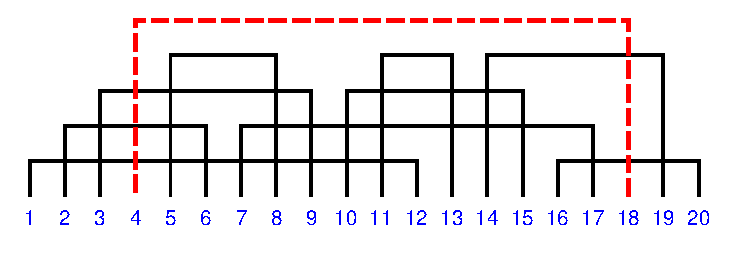
\includegraphics[scale=0.8]{Figs/Probability/ints}
\end{figure}

%ё
\section*{Решения и комментарии}

\subsubsection*{Потерянный посадочный талон}% (THE LOST BOARDING PASS)

Давайте дождёмся когда сотый пассажир поднимется на борт. 
Оставшееся место будет либо то, что указано на его посадочном талоне, либо место первого пассажира.
Все остальные места заняты пассажирами согласно посадочным талонам или теми, что сели первыми.

Так как на каждом шаге ни одному из этих двух мест не было дано никакого предпочтения, вероятность того, что сотый пассажир сядет на своё место равна $50\%$.
\heart

Приведённое здесь рассуждение аналогично тому, что используется, скажем, при подсчёте шансов в Крэпсе (разновиднось игры в кости с двумя кубиками).
После того, как вы выбросили «пойнт»,
(то есть в сумме два кубика дали 4, 5, 6, 8, 9 или 10), вы продолжаете бросать кости до тех пор, пока не выпадет 7 или тот же пойнт.
Чтобы определить вероятность выигрыша (повторный выброс пойнта), вы предполагаете, что следующий бросок последний, и рассчитываете соответственно.
Например, если ваш пойнт --- 5, ваши шансы --- 4 из 10 (потому что имеется 4 способа выбросить 5 и 6 способов выбросить 7).
В случае с потерянным посадочным талоном, один из 99 пассажиров в конце концов сядет на место первого или место сотого, в этот момент оба этих места выбираются с равной вероятностью. 

\medskip

Источник: Дружеские беседы.
В данном случае я услышал эту задачу на конференции «Gathering for Gardner V».
Приведённая здесь версия предоставлена Анде Холройдом. % (Ander Holroyd). %???

\subsubsection*{Все грани кубика}% (ROLLING ALL THE NUMBERS)

Данная классическая задача демонстрирует два важных принципа: среднее время ожидания и линейность математического ожидания. %???
Предположим, вы повторяете эксперимент, вероятность успеха которого равна $p$.
Как долго надо вам ждать успешного исхода? Вы можете вычислить это значение как сумму
\[\sum_{n=1}^\infty n(1-p)^np=1/p,\]
но это не выглядит особо убедительно с интуитивной точки зрения.
Лучше представим, что эксперимент повторяется $n$ раз, и $n$ настолько большое, что доля успешных экспериментов сколь угодно близка к $p$ (закон больших чисел).
Вы можете думать об этих $n$ испытаниях, как об отдельных сериях по $pn$ экспериментов, где каждый эксперимент завершается успехом.
Их средняя длина равна $n/(np)=1/p$.

В задаче требуется выбросить все шесть цифр, и ключевой момент состоит в том, чтобы разбить этот процесс на шесть этапов.
Среднее время, что потребуется для завершения всех этапов, будет тогда равно сумме средних времён каждого этапа.
Теперь, как известно, если проследить за числом различных цифр, которые уже выпали, то первое значение этого числа будет равно 1 (после первого броска) и оно будет, шаг за шагом, увеличиваться на единицу, пока не достигнет 6.
Положим, «этап номер $k$» --- это период, в течении которого уже были выброшены $k-1$ различных цифр, и мы ожидаем появления $k$-той.

Вероятность успеха на этапе номер $k$ равна, всего лишь, числу цифр, ещё не выпавших на кубике, а именно $6-(k-1)$, разделённому на $6$;
значит средняя длина этапа номер $k$ равна $6/(6-k+1)$.
Из этого следует, что среднее время для всего процесса будет
\[\frac66+\frac65+\frac64+\frac63+\frac62+\frac61=14{,}7.\]
\heart

Пожалуй, стоит отметить, что результат был бы совсем другим, если бы мы бросали шесть кубиков одновременно и ожидали, когда выпадут все цифры сразу при одном броске.
Вероятность успеха равна $6{\cdot}5{\cdot}4{\cdot}3{\cdot}2{\cdot}1/6^6$ (смотри, например, последнюю задачу в предыдущей главе), что приблизительно равно $0{,}0154321$.
Следовательно, среднее время ожидания будет состоять из $64{,}8$ попыток, это довольно долго, учитывая, что при одной попытке мы бросаем 6 кубиков одновременно.

\subsubsection*{Нечётная череда решек}% (ODD STREAK OF HEADS)

Данная задача была предложена, но не была использована, на ММО в начале 80-х.%
\footnote{Смотри Murray Klamkin, \emph{International Mathematical Olympiads, 1978--1985} Mathematical Association of America, 1986.}
Она идёт в паре с предыдущей задачей, но здесь надо больше думать.

\medskip

Если мы подсчитаем вероятность того, что мы выбрасываем решку сразу же нечётное число раз, и потом орла, мы получаем 
\begin{align*}\mathbb{P}(\textsc{ро})+ \mathbb{P}(\textsc{ррро})+ \mathbb{P}(\textsc{ррррро})+\dots&=
\\
=(\tfrac12)^2+(\tfrac12)^4+(\tfrac12)^6+\dots&=\tfrac13.
\end{align*}

Если так не удаётся, то есть выпадает орёл (после чётного числа решек), мы должны начинать сначала.
Таким образом, в среднем, нам понадобится три подобных эксперимента.
Но мы хотим посчитать количество бросков, а не экспериментов.

К счастью, мы можем воспользоваться другим свойством математического ожидания:
Если имеется произвольное число $n$ объектов, чья средняя величина равна $s$, тогда средняя общая величина всех объектов равна $s$, помноженному на среднее значение $n$.
Каждый из экспериментов (успешный или нет) заканчивается, когда появляется первый орёл, таким образом, среднее число бросков на эксперимент $1:\tfrac12=2$.
Из этого следует, что
решением задачи будет $2{\cdot}3=6$ бросков.\heart

Есть более красивый способ решения этой задачи.
Пусть ответ равен $x$.
Если мы начинаем с \textsc{о} или \textsc{рр}, то для достижения успеха нам предстоит сделать в среднем ещё $x$ бросков.
Если мы начинаем с \textsc{ро}, то это уже успех.
Отсюда
\[x=\tfrac12 \cdot(1+x)+\tfrac14 \cdot(2+x)+\tfrac14 \cdot2.\]
Что нам даёт $x=6$.

\subsubsection*{Три кубика}% (THREE DICE)

Вообще-то, эта игра предлагаются в некоторых казино, в Америке она называется чак-э-лак или бёрд кейдж%
\footnote{англ. Bird Cage --- \emph{птичья клетка}; кубики в этой игре обычно бросаются в клетке}. %???
Справедливо заявить, что уже один этот факт сам по себе является доказательством без вычислений того, что игра идёт в пользу казино.

Однако есть довольно красивый математический способ показать это, и он применим также и к другим азартным играм.
Представим себе, что у нас шесть игроков, все ставят по 1 доллару на разные числа, и затем бросаются кубики.
Казино никогда не проигрывает!
Если выпадают три различных числа, крупье забирает 3 доллара у проигравших и отдаёт их выигравшим.
В остальных случаях крупье забирает 4 или 5 долларов, отдавая выигравшим только 3.\heart

Итак, игра идёт в пользу казино, если игроки делают ставки подобным образом.
Но, значит ли это, что она \emph{всегда} в пользу казино?
Да, значит --- статистически, казино выигрывает или проигрывает не независимо от того, кто как и сколько ставит.

Конечно, совсем несложно определить напрямую, что чак-э-лак --- дело проигрышное.
Вероятность того, что выпадут три разных числа равна $6{\cdot}5{\cdot}4/6^3=5/9$.
Игрок, делающий ставку, рискует уже здесь, так как вероятность того, что его число одно из выпавших, равна $1/2$.
С вероятностью $1/36$ на всех кубиках выпадет одно и тоже число;
и тут игрок получает $3$ доллара с вероятностью $1/6$ и теряет 1 доллар всё остальное время, средний проигрыш будет $1/3$ доллара.
И, наконец, оставшиеся $5/12$ времени игрок выигрывает $2$ доллара с вероятностью $1/6$, и теряет $1$ доллар с вероятностью $2/3$, в среднем он проигрывает $1/6$ доллара.
В общем, его потери составят $1/36{\cdot}1/3 + 5/12{\cdot}1/6 = 17/216$; то есть, примерно, $8$ центов с доллара.

\medskip

Игру можно сделать честной, давая игроку 3 доллара вместо 2 при выпадении двух одинаковых чисел 
и 5 долларов вместо 3, когда выпадают 3 одинаковых числа.

\medskip

Эта задача впервые появилась в «Энциклопедии головоломок» Сэма Лойда, под редакцией Сэма Лойда II, 1914\footnote{\emph{Sam Loyd’s Cyclopedia of 5000 Puzzles, Tricks, and Conundrums,} edited by Sam Loyd II, 1914}.
Сэм Лойд (старший), 1841---1911, хорошо известен многим читателям как непревзойдённый мастер занимательных задач и величайший американский головоломщик.

\subsubsection*{Намагниченные доллары}% (MAGNETIC DOLLARS)

Большинство людей предположат, что урна с меньшим количеством сюзанн практически ничего не стоит.
И действительно, недавно сидя в ресторане с профессиональными математиками, в ответ на данный вопрос только один был готов предложить 100 долларов, остальные же давали не больше 10.

На самом деле, эта урна стоит, в среднем, хорошую четверть миллиона долларов.
Вероятность распределения конечного содержимого для двух урн однородна.
Вероятность того, что, скажем, в первой урне в конце окажется только одна сюзанна такая же, как и вероятность того, что там будет 451 382 сюзанны.

Это легко доказывается по индукции, но я считаю гораздо интереснее приведённую ниже аналогию с тасованием карт.
Представим себе колоду из 999 999 карт, из которых только одна --- красная.
Перетасуем их очень хорошо следующим способом.
Положим красную карту на стол.
Теперь берём вторую карту (любую) и кладём её с одинаковой вероятностью на или под красную карту.
Есть три варианта, куда можно поместить следующую карту, с одинаковой вероятностью выбираем один из них и вставляем карту.
Когда последняя карта добавлена, на столе у нас --- идеально перетасованная колода карт.

Но заметьте: когда сверху красной карты находятся $x-1$ карта, а снизу $y-1$, то вероятность того, что следующая карта окажется над красной равна $x/(x+y)$.
Таким образом, карты сверху красной карты ведут себя также, как сюзанны (не считая начальной) из первой урны, а карты снизу --- как из второй.

Из того, что в конечной колоде красная карта может с равной вероятностью оказаться на любой высоте, следует однородность распределения для сюзанн.\heart
 
Задачу (парадокс?) о намагниченных долларах иногда называют «Урной Пойа»,\footnote{Смотри N. Johnson and S. Kotz, \emph{Urn Models and Their Applications: An Approach to Modern Discrete Probability Theory,} Wiley, New York, 1977.} по имени великого математика, популяризатора науки и любителя головоломок Дьёрдя П\'{о}йа, 1887---1985.
Нетрудно показать, что если подбрасывается бесконечное количество сюзанн, то в пределе с вероятностью, равной 1, процент сюзанн, попавших в первую урну, задаётся однородным распределением на единичном интервале.

\subsubsection*{Торговля вслепую}% (BIDDING IN THE DARK)

Вы не должны делать предложение.
Если вы предложите $x$ долларов, то ожидаемая стоимость приборчика для хозяина, при условии, что \emph{он его продаёт}, будет равна $x/2$ доллара.
Следовательно, для вас ожидаемая стоимость приборчика, если вы его получите, будет равна $1{,}8 {\cdot} x/2=0{,}9{\cdot}x$ долларов.
Таким образом, в среднем, вы теряете деньги, если покупаете приборчик и, конечно же, ничего не теряете и не выигрывайте, если не покупаете.
Так что глупо предлагать.\heart

Источник: Майя Бар Хиллел, университет в Иерусалиме.

\subsubsection*{Случайные интервалы}% (RANDOM INTERVALS)

У этой задачи любопытная история.
Моему коллеге (Эду Шнайнерману из университета Джона Хопкинса) и мне нужно было решить эту задачу, чтобы вычислить диаметр так называемого \emph{случайного интервального графа}. 
Вначале мы доказали, что асимптотическое значение этой вероятности равно $2/3$.
Потом, много и беспорядочно интегрируя, нашли, что вероятность того, что найдётся интервал, который пересекает все остальные \emph{в точности} равна $2/3$ (для любого числа интервалов начиная с двух).

Джойс Джастич, %(Joyce Justicz)
будучи в то время моим аспирантом в университете Эмори, придумал следующее комбинаторное доказательство.

Предположим, конечные точки интервалов выбираются из множества $\{1,2,\dots,2n\}$.
Обозначим $2n-4$ из их концов символами $A(1)$, $B(1)$, $A(2)$, $B(2),\dots, A(n-2)$, $B(n-2)$ согласно следующему рекурсивному правилу.
Будем говорить что точки $\{n+1, \dots , 2n\}$ лежат с правой стороны, а точки $\{1, \dots , n\}$ --- с левой.
Положим $A(1)=n$ и $B(1)$ --- парная ей точка.
Допустим, мы уже выбрали точки до $A(j)$ и $B(j)$. 
Если $B(j)$ лежит с левой стороны, тогда $A(j+1)$ выбирается самой левой из невыбранных ещё точек правой стороны, и $B(j+1)$ --- её пара.
Если $B(j)$ лежит с правой стороны, тогда $A(j+1)$ выбирается самой правой из необозначенных ещё точек левой стороны, и снова $B(j+1)$ --- её пара.

Если $A(j) < B(j)$, мы говорим, что интервал «ушёл направо», в обратном случае --- он «ушёл налево».
Точки, обозначенные $A({\cdot})$ будем называть внутренними концами интервала, остальные --- внешними.

\begin{figure}[h!]
\centering
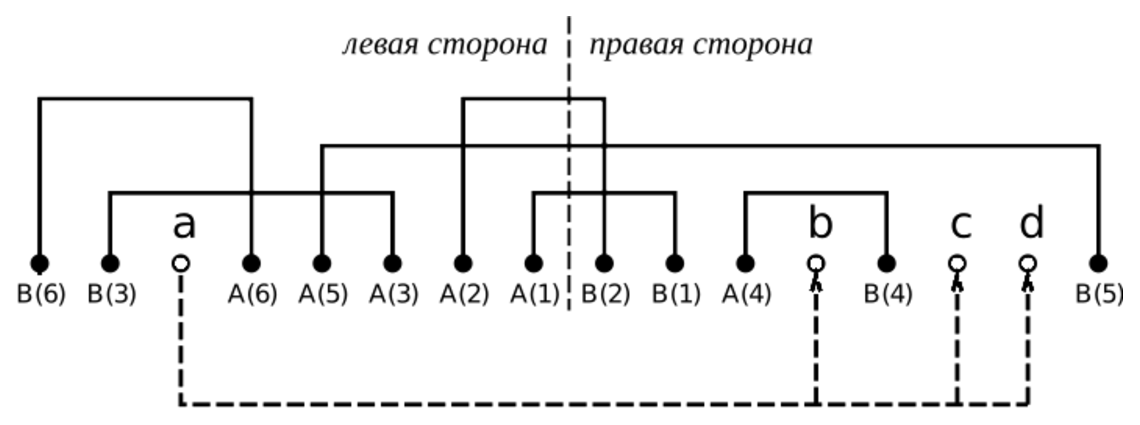
\includegraphics[scale=0.55]{Figs/Probability/labeling-ru}
\end{figure} 

Используя индукцию по $j$, легко доказать, что после того, как выбраны $A(j)$ и $B(j)$, либо одинаковое количество точек было выбрано на каждой из сторон (в случае если $A(j) < B(j)$), либо на левой стороне было выбрано на две точки больше (в случае если $A(j) > B(j)$).

После того, как мы обозначили точки $A(n-2)$ и $B(n-2)$, остаётся четыре необозначенных точки концов интервалов, назовём их $a<b<c< d$.
Мы утверждаем, что из трёх равновероятных способов разбиения этих точек на пары, два приведут к «больш\'{о}му» интервалу, пересекающему все остальные, а один способ --- нет.

В случае если $A(n-2) < B(n-2)$, точки $a$ и $b$ находятся слева, а $c$ и $d$ --- справа;
в противном случае только $a$ находится слева.
В любом случае, все внутренние концы интервалов лежат между точками $a$ и $c$, иначе одна из них была бы выбрана.
Из этого следует, что интервал $[a,c]$ пересекает все остальные, и точно также $[a,d]$.
То есть, если $a$ не в паре с $b$, то у нас большой интервал.

Допустим, напротив, что наши пары именно $[a, b]$ и $[c, d]$.
Ни одна из них не может быть большим интервалом, так как они не пересекаются с друг другом.
Предположим теперь, что существует другой большой интервал, скажем $[e,f]$ с концами $A(j)$ и $B(j)$.

Если точки $a$ и $b$ находятся слева, внутренние концы $A(j)$ лежат между $b$ и $c$, таким образом $[e, f]$ не может пересекать оба интервала $[a, b]$ и $[c, d]$, что противоречит нашему предположению.

В оставшемся случае, так как $[e, f]$ пересекает $[c, d]$, $f$ является внешним концом интервала. 
В этом случае $f=B(j)$, то есть отрезок $[e, f]$ ушёл направо.
Поскольку последняя выбранная пара точек ушла налево, существует $k>j$, для которого $A(k)>B(k)$ и $A(k-1)<B(k-1)$.
В этом случае $A(k)$ лежит слева и значит $A(k) < A(j)$, так как $A(k)$ --- левосторонняя внутренняя точка, выбранная позже.
Тогда $[A(j), B(j)]$ не пересекает $[B(k), A(k)]$; это последнее противоречие доказывает наше утверждение.
\heart

Используя данное рассуждение с чуть большей аккуратностью, можно доказать, что 
для $k < n$ , вероятность того, что в семействе случайных $n$ интервалов найдётся, по меньшей мере, $k$ интервалов, которые пересекают все остальные, равна
\[\frac{2^k}{\binom{2k+1} k}\]
и она не зависит от $n$.
Здесь $\binom n k$ означает \emph{биноминальный коэффициент}, то есть число подмножеств размера $k$ из множества размера $n$, и он равен $n(n-1)(n-2)\cdots(n-k+1) /(k(k-1)(k-2)\cdots1)$.

\chapter*{Геометриуя}

\epigraph{Уравнения --- просто скучная часть математики.
Я пытаюсь смотреть на мир с точки зрения геометрии.}{---Стивен Хокинг (1942---2018)}

Классическая геометрия в двух- или трёхмерном пространстве является, безусловно, неисчерпаемым источником для составителей задач. %???безусловно в начало???
Но мы хотим головоломок, а это не те задачи, которые бы Евклид включил в свой Том II.
Поэтому вас не будут просить доказать, что $AB=CD$, или что один треугольник конгруэнтен другому.

Но к счастью, существует огромное множество очаровательных геометрических задач, отвечающих нашей цели. 
Задача, которую мы разберём в качестве примера, появилась в 1980 году на подготовительном  школьном экзамене, %(Preliminary Scholastic Aptitude Exam),
где, к стыду составителей из экзаменационного комитета по образованию, %(англ. Educational Testing Service),???может всё же убрать "по образованию" 
утверждённый правильным ответ оказался неверен.
И один смелый ученик, получив результат экзамена, обратился в комитет с аппеляцией.
К нашей большой радости, правильное решение являет собой  чудесное интуитивное доказательство.
(Хочу заметить, что впоследствии был создана специальная группа, в которой  трудился и ваш автор, для анализа экзаменационных заданий по математике.)

\subsection*{Склеивание пирамид}% (GLUING PIRAMIDS)

Пирамида с квадратным основанием, имеющая рёбра единичной длины, и пирамида с треугольным основанием (тетраэдр), также с рёбрами единичной длины, склеены вместе по треугольным граням.

Сколько граней имеет полученный многогранник?

\paragraph{Решение:}

Пирамида с квадратным основанием имеет пять граней, тетраэдр --- четыре.
Так как две грани склеены вместе, у получившегося многогранника будет $7=4+5-2$ граней, правильно?
Это, очевидно, была преполагаемая линия рассуждений.
Составителю задачи могло бы прийти в голову, что, в принципе, пара прилегающих граней из разных многогранников, может в после склейки оказаться в одной плоскости.
Таким образом, они сольются в одну грань, что уменьшит ответ.
Но, несомненно, такое совпадение должно быть исключено.
Ведь эти два многогранника даже не одинаковой формы.

Но на самом деле, так и случается (дважды):
склеенный многогранник имеет пять граней.
Вы можете вообразить себе такую картину: две пирамиды с квадратным основанием стоят на столе основаниями вниз и примыкают друг к другу по ребру основания.
Теперь, соединив вершины пирамид воображаемой линией, отметим, что длина полученного отрезка равна единице, как и все рёбра пирамиды.

Таким образом, между двумя пирамидами с квадратным основанием помещается правильный тетраэдр.
Две плоскости, каждая из которых содержит по треугольной грани от каждой из двух пирамид, также содержит и грань тетраэдра.
Отсюда результат.
\heart

(Если вам затруднительно это представить, посмотрите картинку ниже.)

Данное доказательство, иногда называемое «палаточным решением», появилось в 1982 в статье Стивена Янга.%
\footnote{Steven Young “The Mental Representation of Geometrical Knowledge”, in the Journal of Mathematical Behavior.}

\begin{figure}[h!]
\centering
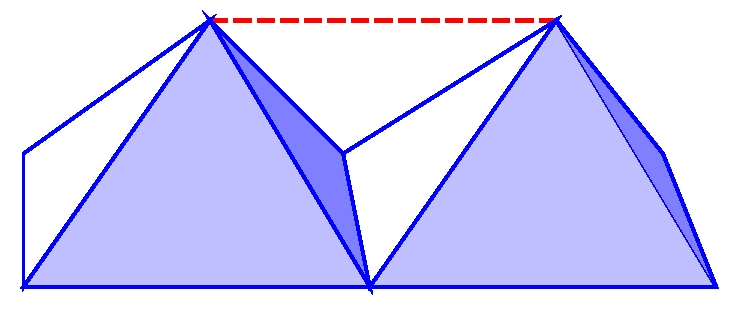
\includegraphics[scale=0.55]{Figs/Geometry/pyrs}
\end{figure} 

Одна из задач, приведённых ниже, имеет «доказательство без слов» --- достаточно одного рисунка.
Посмотрим, сможете ли вы догадаться, которая.

\subsection*{Окружности в пространстве}% (CIRCLES IN SPACE)

Возможно ли трёхмерное пространство разбить на окружности? 

\subsection*{Магия кубов}% (MAGIC WITH CUBES)

Можно ли протащить куб сквозь отверстие в кубе меньшего размера?

\subsection*{Красные и синие точки}% (RED POINTS AND BLUE POINTS)

На плоскости дано $n$ красных и $n$ синих точек, при этом никакие три точки не лежат на одной прямой.
Докажите, что их можно разбить на пары таким образом, что отрезки, соединяющие каждую красную точку с соответствующей ей синей, не пересекаются.

\subsection*{Прямая через две точки}% (LINE THROUGH TWO POINTS)

Пусть $X$ --- конечное множество точек на плоскости, не все из которых лежат на одной прямой.
Докажите, что существует прямая, проходящая ровно через две точки из $X$.

\subsection*{Пары на максимальном расстоянии}% (PAIRS AT MAXIMUM DISTANCE)

И снова, $X$ --- конечное множество точек на плоскости.
Положим, $X$ содержит $n$ точек и максимальное расстояние между любыми двумя точками из них равно $d$.
Докажите, что существует максимум $n$ пар точек из $X$, расстояние между которыми равно $d$.

\subsection*{Монах на горе}% (MONK ON A MOUNTAIN)

В понедельник на рассвете монах начинает восхождение на гору Фудзияма и с приходом ночи достигает вершины.
Он проводит ночь на вершине горы и на следующее утро пускается в обратный путь, добираясь до подножия горы на закате солнца.

Докажите, что в определённый  момент времени во вторник,  монах окажется точно на той же высоте, на какой  он был в точно такое же время в понедельник.

\subsection*{Раскраска многогранника}% (PAINTING THE POLYHEDRON)

Предположим, грани многогранника $P$ раскрашены в красный и зелёный цвет так, что каждая красная грань окружена зелёными, и при этом суммарная площадь красных граней превосходит суммарную площадь зелёных.
Докажите, что в многогранник $P$ невозможно вписать сферу.

\subsection*{Круглые тени}% (CIRCULAR SHADOWS)

Два круга являются проекциями некоторого тела на две плоскости.
Докажите, что радиусы этих кругов равны.

\subsection*{Полоски на плоскости}% (STRIPS IN THE PLANE) 

Назовём «полоской» часть плоскости между двумя параллельными прямыми.
Докажите, что нельзя покрыть плоскость множеством полосок, суммарная ширина которых конечна.

\subsection*{Ромбики в шестиугольнике}% (DIAMONDS IN HEXAGON)

Из треугольной решётки вырезали большой правильный шестиугольник и замостили его «ромбиками» (парами  треугольников, склееных по стороне).
Ромбики разбиваются на три вида в зависимости от их ориентации.
Докажите, что в замощении присутсвует равное количество ромбиков каждого вида.

\begin{figure}[h!]
\centering

\includegraphics[scale=0.55]{Figs/Geometry/hex}
\end{figure}

\subsection*{Замощение ромба}% (RHOMBUS TILING)

Давайте попробуем ещё раз, но плитки будут больше и больше будет количество сторон.

Рассмотрим $\binom n2$ различных ромбов, образованных парами непараллельных сторон правильного $2n$-угольника.
Замостите ими $2n$-угольник, используя параллельный перенос ромбов
и докажите, что каждый ромб может использоваться ровно один раз в любом таком замощении.

\subsection*{Векторы на многограннике}% (VECTORS ON A POLYHEDRON)

Каждой грани многогранника соответствует вектор, перпендикулярный грани, направленный вовне, и имеющий длину, равную площади грани.
Докажите, что сумма этих векторов равна нулю.

\subsection*{Три окружности}% (THREE CIRCLES)

Назовём фокусом двух окружностей точку пересечения двух прямых, каждая из которых является касательной к обеим окружностям, но не проходит между ними.
Таким образом, три окружности различных радиусов (не лежащих в друг друге)
определяют три фокуса.
Докажите, что эти три фокуса лежат на одной прямой.

\begin{figure}[h!]
\centering
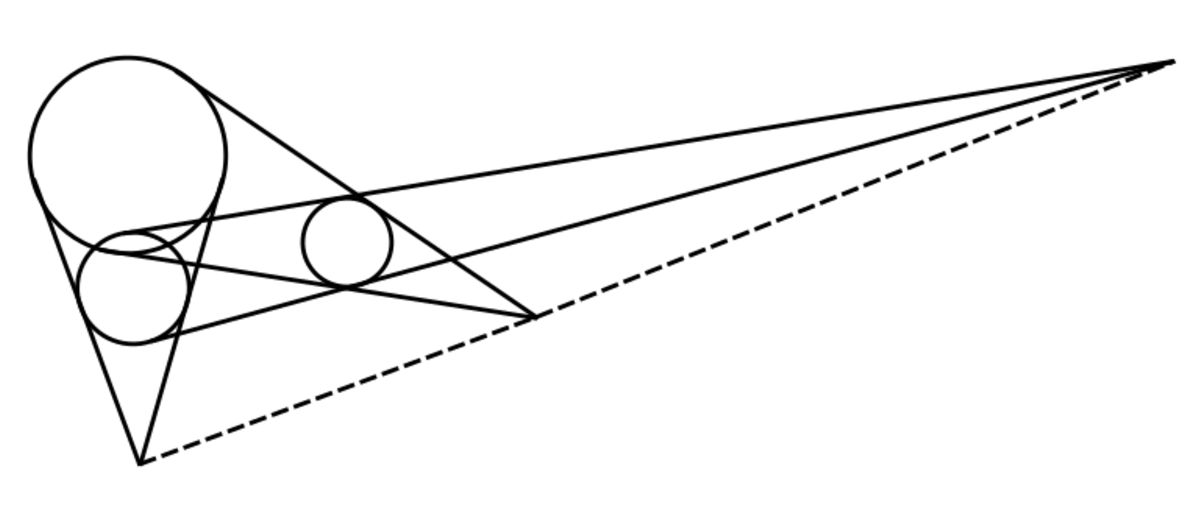
\includegraphics[scale=0.5]{Figs/Geometry/foci}
\end{figure} 

\subsection*{Сфера и четырёхугольник}% (SPHERE AND QUADRIATERAL)

Пространственный четырёхугольник касается всеми сторонами сферы.
Докажите, что все точки касания лежат в одной плоскости.

\medskip

Последняя задача является небольшой экскурсией в топологию и иерархию бесконечностей.

\subsection*{Восьмёрки на плоскости}% (FIGURES 8S IN THE PLANE)

Сколько непересекающихся топологических «восьмёрок» можно нарисовать на плоскости?

\begin{figure}[h!]
\centering
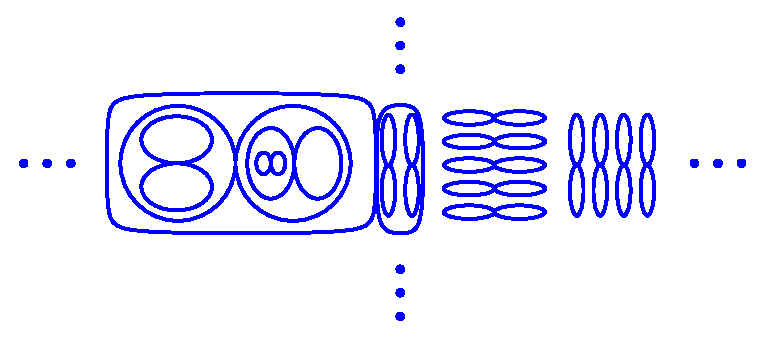
\includegraphics[scale=0.5]{Figs/Geometry/eights}
\end{figure} 

\section*{Решения и комментарии}

\subsubsection*{Окружности в пространстве}% (CIRCLES IN SPACE)

Да.
Построим на $XY$-плоскости окружности радиуса $1$, центр кoторых лежит на оси $Х$ в точках $1$ по модулю $4$ (то есть точки $\dots, (-7,0)$, $(-3,0)$, $(1,0)$, $(5,0)$, $(9,0),\dots$).
Обратите внимание, что каждая сфера с центром в начале координат пересекает эти окружности ровно в двух точках.
Остаток каждой такой сферы --- это объединение окружностей.
\heart

\begin{figure}[h!]
\centering

\includegraphics[scale=0.7]{Figs/Geometry/ring}
\end{figure} 

Существуют и другие способы доказательства этого факта, например, с помощью торов, но я не знаю подхода более простого и элегантного, чем приведённый выше.

Эту милую задачу на разбиения я впервые услышал от Ника Пиппенгера, %(Nick Pippenger)
профессора информатики Принстонского университета.

\subsubsection*{Магия кубов}% (MAGIC WITH CUBES)

%??? путает проекцию и сечение

Да, это можно сделать.
Для того, чтобы протащить единичный куб сквозь отверстие в другом единичном кубе, достаточно найти проекцию (второго) куба, содержащую внутри себя единичный квадрат.
Тогда во втором кубе можно проделать сквозное квадратное отверстие %(square cylindrical) 
со стороной чуть больше единицы, чтобы можно было протащить первый куб.

Можно сделать то же самое, с меньшим допуском, если второй куб только слегка меньше первого.

Самую простую (но не единственную) проекцию, которую можно использовать --- это правильный шестиугольник.
Можно увидеть этот шестиугольник, если посмотреть на куб так, что одна из вершин будет посредине.
Формально говоря, это проекция на плоскость, перпендикулярную его диагонали.

Пусть $A$ --- проекция одной из видимых граней на плоскость.
Мы видим, что её большая диагональ имеет ту же длину ($\sqrt{2}$), что и диагональ единичного куба, так как в этом направлении проекция не сокращает длину.
Если сдвинуть $A$ к центру шестиугольника и затем растянуть её до единичного куба $B$, то вытянутые углы $B$ не достанут до вершин шестиугольника (так так расстояние между противоположными вершинами шестиугольника превышает расстояние между противоположными сторонами).

\begin{figure}[h!]
\centering
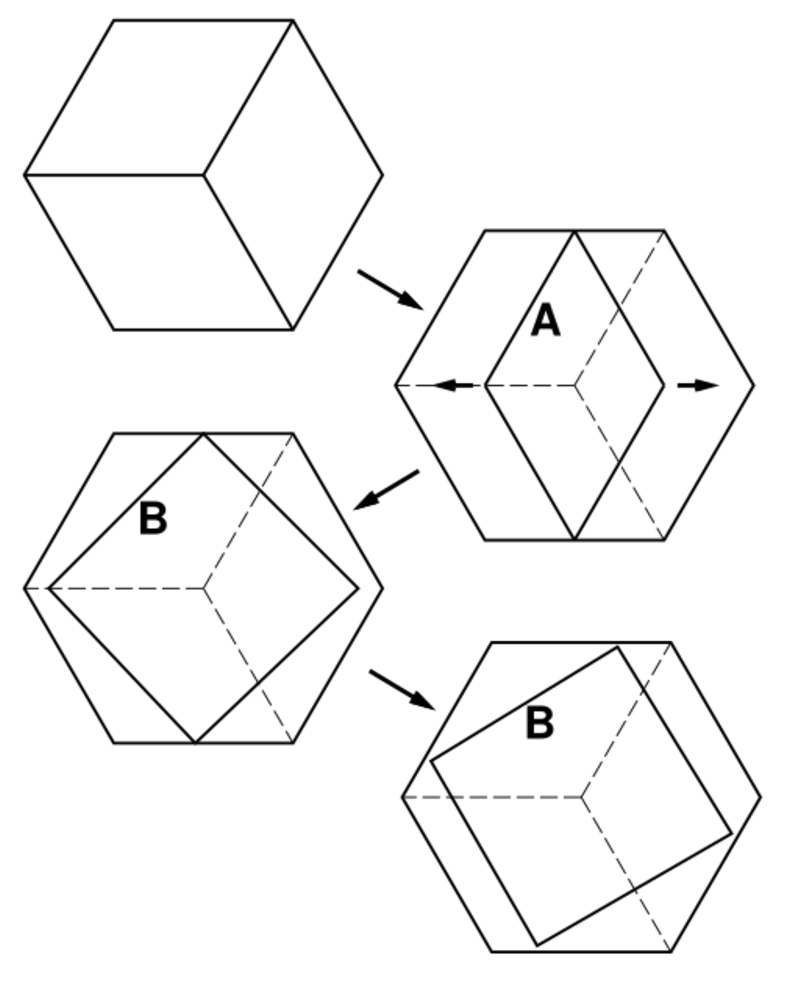
\includegraphics[scale=0.7]{Figs/Geometry/pass}
\end{figure}

Значит, если слегка повернуть квадрат $B$, то он окажется строго внутри шестиугольника.\heart

Об этой очаровательной задаче, появлявшейся в колонке Мартина Гарднера, мне напомнил Григорий Гальперин из университета Восточного Иллинойса.

\subsubsection*{Красные и синие точки}% (RED POINTS AND BLUE POINTS)

Среди всех возможных разбиений, возьмём то, при котором общая длина всех $n$ отрезков минимальна.
Мы утверждаем, что такое разбиение не будет иметь пересечений.
Действительно, если бы отрезок $uv$ пересекал отрезок $xy$, то эти отрезки были бы диагоналями выпуклого четырёхугольника $uyvx$, %???ошибка в книжке
и, по неравенству треугольника, заменив диагонали на стороны $uy$ и $xv$, мы бы уменьшили общую длину отрезков.\heart

Технику, которой мы здесь воспользовались, состоящую в нахождении нужного объекта, минимизируя или максимизируя некую величину, иногда называют вариационным методом, и он, как знают многие читатели, чрезвычайно полезен.
Следующая задача предлагает ещё один пример его применения.

Источник : Олимпиада Патнема 1960-х.

\subsubsection*{Прямая через две точки}% (LINE THROUGH TWO POINTS)

Эта знаменитая гипотеза была сформулирована Джеймсом Сильвестром в 1893 году.
Первое доказательство найдено Тибором Галлаи, %(Tibor Gallai).
но доказательство, приведённое ниже, данное в 1948 году Л. М. Келли,\footnote{L. M. Kelly American Mathematical Monthly, Vol.55} 
часто упоминалось Палoм Эрдёшем, как пример доказательства из «Книги».

\begin{figure}[h!]
\centering
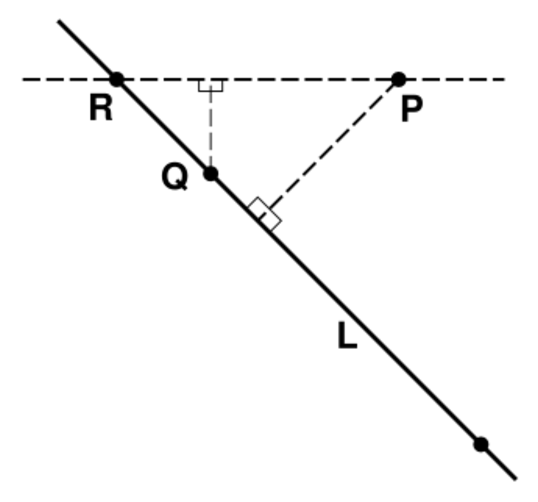
\includegraphics[scale=0.7]{Figs/Geometry/kelly}
\end{figure}

Предположим, что каждая прямая, проходящая через две точки множества $X$, содержит, по меньшей мере, три точки из $X$.
Идея состоит в том, чтобы рассмотреть прямую $L$ и точку $P$, не лежащую на $L$, такие что расстояние от $P$ до $L$ минимально.

Поскольку $L$ содержит, по меньшей мере, три точки из $X$, две из них, скажем, $Q$ и $R$, лежат с одной стороны от перпендикуляра, опущенного из точки $P$ на прямую $L$.
Но тогда, если $R$ --- дальняя точка, то $Q$ находится ближе к прямой $PR$, чем $P$ к $L$ --- противоречие.\heart

\subsubsection*{Пары на максимальном расстоянии}% (PAIRS AT MAXIMUM DISTANCE)

Для решения данной задачи из олимпиады Патнема 1957 года, будет полезно следующее наблюдение: если $A,B$ и $C,D$ --- две «максимальные пары» (то есть пары точек из $X$, расстояние между которыми равно $d$), тогда отрезки $AB$ и $CD$ пересекаются (иначе одна из диагоналей прямоугольника $ABCD$ будет иметь длину, превышающую $d$).

Предположим, что утверждение задачи неверно, и пусть наименьший контрпример имеет размер $n$.
Поскольку максимальных пар больше, чем $n$, и каждая состоит из двух точек, то должна существовать такая точка $P$, которая принадлежит трём максимальным парам (пусть это будут пары с точками $A$, $B$, $C$).
Каждые два из отрезков $PA$, $PB$ и $PC$ должны в точке $P$ образовывать угол максимум в 60\degree.
Один из этих отрезков, скажем, $PB$, %???ошибка в книжке
должен лежать между двумя другими.

Но тогда точке $B$ будет довольно сложно образовать максимальную пару с какой-либо другой точкой, так как, если $BQ$ была бы максимальной парой, то отрезок $BQ$ должен бы был пересекать и $PA$, и $PC$, что невозможно.
Значит, можно выбросить $B$ из множества $X$, теряя при этом только одну максимальную пару и получая таким образом меньший контрпример.
Это противоречие завершает доказательство.\heart

\subsubsection*{Монах на горе}% (MONK ON A MOUNTAIN)

Пожалуй, самое лёгкое решение --- это представить себе, что у монаха есть близнец, которому даны указания взобраться на гору во вторник утром точно тем же путём, каким шёл монах в понедельник.
Тогда монах должен встретить близнеца по дороге вниз, или, если они идут разными тропами, оказаться в какой-то момент на одной с ним высоте.\heart

(Возможно, эта задача показалась вам слишком лёгкой, не волнуйтесь, гораздо более сложная её версия ожидает вас в Главе 11 --- «Крепкие орешки»)

На эту древнюю задачу можно смотреть как на пример применения теоремы о промежуточном значении --- очень полезной теоремы утверждающей, что непрерывная функция обязана принять все свои промежуточные значения.
В нашем случае функцией можно выбрать разность между высотой, на которой оказался монах в определённое время дня в понедельник, и высотой, на которой он был в то же самое время дня во вторник.
Начальное значение функции будет отрицательным (примерно минус высота горы Фудзияма), а конечное значение --- положительным, таким образом, в некой точке функция должна обратиться в ноль.

Геометрически, вы можете представить, что высота, на которой находился монах в каждый из дней, представлена графиком, и два графика наложены друг на друга.
Тогда должна существовать точка (или точки), где они пересекаются.

Другими  известными примерами применения теоремы о промежуточном значении являются задачи о том, можно ли вписать озеро Мичиган в квадрат, и можно ли  разрезать сэндвич (плоскостью) так, чтобы разделить ветчину, сыр и хлеб точно пополам.

\subsubsection*{Раскраска многогранника}% (PAINTING THE POLYHEDRON)

Предположим, что сфера вписана в $P$, триангулируем грани $P$, используя точки касания сферы.
Тогда треугольники по обе стороны любого ребра конгруэнтны, и, значит, имеют одинаковую площадь.
В каждой такой паре не более одного красного треугольника.
Из этого следует, что площадь красных граней не превосходит площади зелёных, что противоречит условию задачи.\heart

\begin{figure}[h!]
\centering
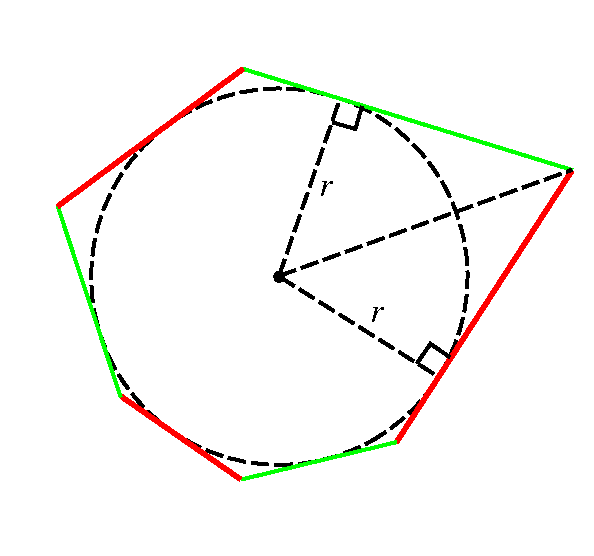
\includegraphics[scale=0.5]{Figs/Geometry/polygon}
\end{figure}%???цвет

Эта задача пришла ко мне от Эмины Солянин %(Emina Soljanin) 
из лабораторий Белла.
На иллюстрации представлена двумерная версия, где стороны и вершины многоугольника заменяют грани и рёбра многогранника $P$.

\subsubsection*{Круглые тени}% (CIRCULAR SHADOWS)

Эта, способная вас смутить, задача, пришла к нам из 5-й Всесоюзной Математической Олимпиады в Риге 1971 года.
Простой способ превратить ваше интуитивное решение в строгое доказательство состоит в следующем: --- поместим тело между двумя плоскостями, перпендикулярными одновременно обеим плоскостям проекций, и начнём их сдвигать.
В  момент, когда они коснутся тела, они пройдут через противолежащие точки каждой из проекций, и расстояние между параллельными плоскостями будет равно общему диаметру проекций.
\heart

\subsubsection*{Полоски на плоскости}% (STRIPS IN THE PLANE) 

Как и предыдущая, данная задача, версия которой появлялась в ранних олимпиадах Патнема, представляет собой ещё один пример «интуитивно очевидного» факта, который всё-таки нужно доказать.

\medskip

Поскольку сложно сравнивать бесконечные величины, имеет смысл сосредоточиться на какой-нибудь конечной части плоскости.
Мы не можем контролировать углы между полосками, так что логично будет рассмотреть круг $D$ радиуса $r$.

Предположим, полоски имеют ширину $w_1$, $w_2,\dots$, которые в сумме дают $1$.
Оказывается, что они не могут покрыть даже круг $D$, при $r=1$.
Действительно, пересечение $D$ с полоской шириной $w$ лежит в прямоугольнике шириной $w$ и длиной $2$, и, следовательно, его площадь меньше $2w$.
Таким образом, площадь, покрытaя полосками внутри $D$, меньше $2$, а площадь $D$, конечно же, $\pi>2$.
\heart 

Доказательство выше говорит, что чтобы покрыть единичный круг, суммарная ширина полосок должна быть больше $\pi/2$, но на самом деле, это можно сделать, только если суммарная ширина хотя бы 2 (в этом случае параллельные полоски дают решение).
Есть очень милое доказательство этого утверждения:
идея в том, чтобы продолжить задачу в 3-мерное пространство, взяв за $D$ сечение единичного шара, проходящее через его центр.
Предположим, круг покрыт полосками, суммарная ширина которых $W$, и пусть $S$ --- одна из полосок шириной, скажем, $w$.
Можно предположить, что либо оба края полоски пересекают $D$, либо один край пересекает и один касается.
Проектируя $S$ вверх и вниз на поверхность шара, мы получаем пояс (или шапочку),
окружающую шар --- чья площадь, здесь вы можете продемонстрировать своё знание анализа, равна 
$2\pi w$, независимо от положения полоски!

Поскольку площадь поверхности шара равна $4\pi$, чтобы её покрыть потребуется $W\ge 2$,
а если не покрыта поверхность шара, то и круг не покрыт.

\subsubsection*{Ромбики в шестиугольнике}% (DIAMONDS IN HEXAGON)

\begin{figure}[h!]
\centering
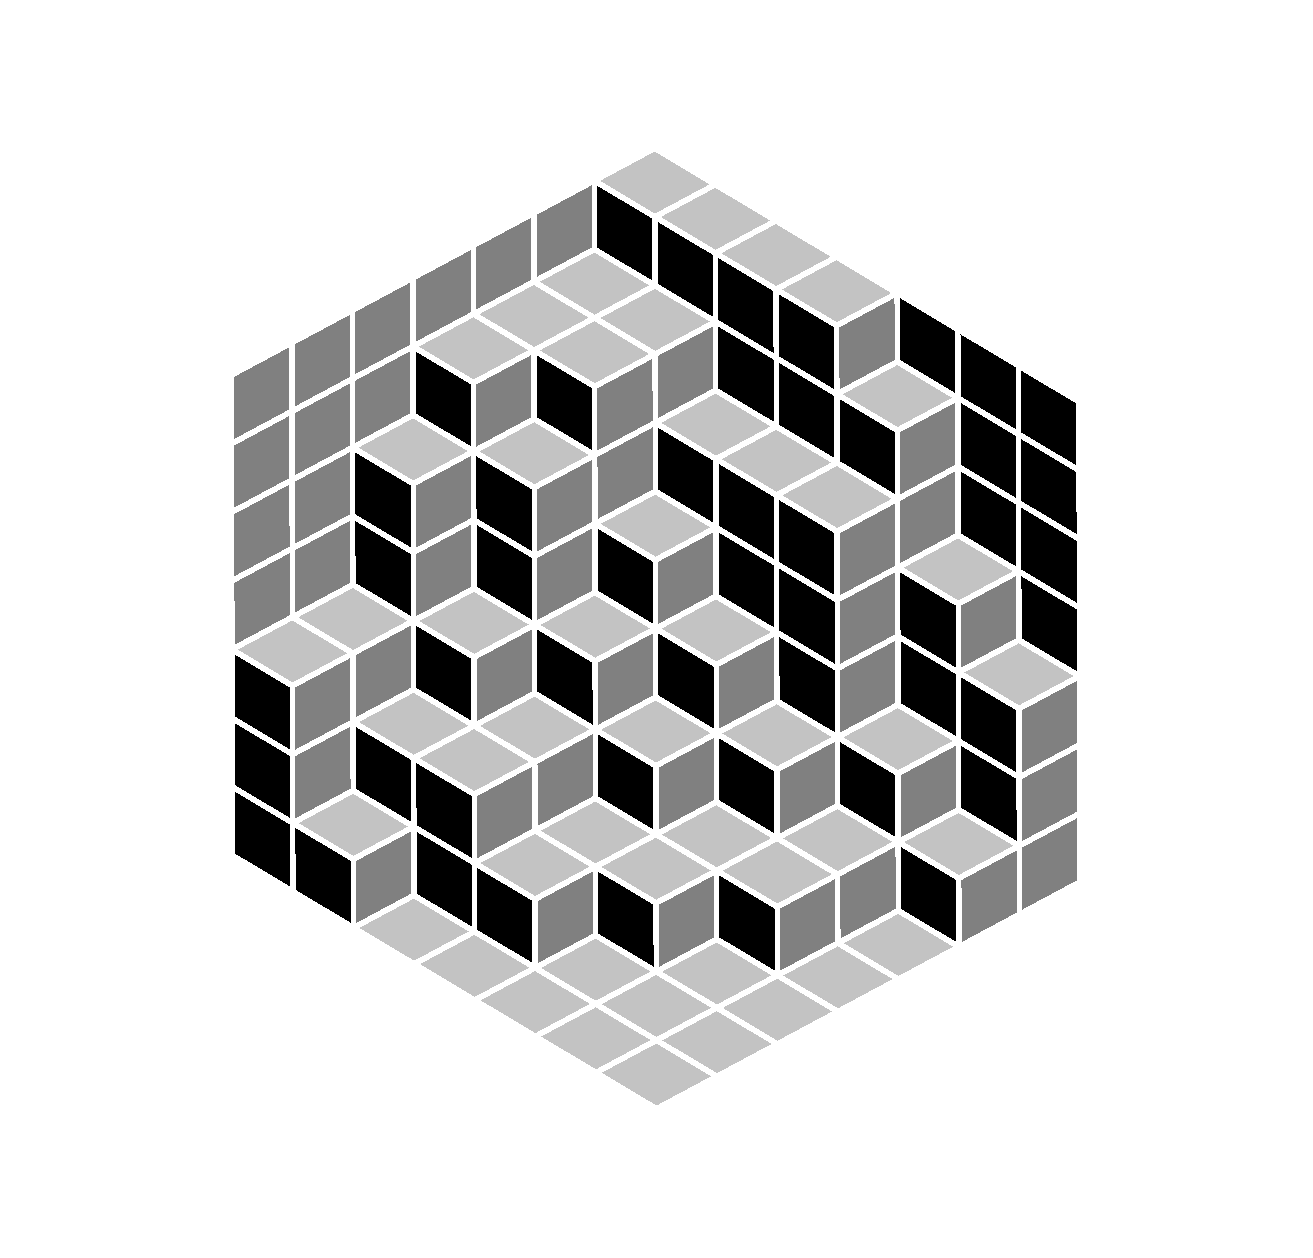
\includegraphics[scale=0.5]{Figs/Geometry/diamonds}
\end{figure}
\heart

Доказательства без слов стали очень популярной темой в журналах «Mathematics Magazine» и «The College Mathematics Journal» Математической aссоциации Америки.
Вы также можете найти эти задачи в книгах Роджера Б. Нелсена.%
\footnote{Proofs Without Words and Proofs Without Words II, by Roger B Nelsen, MAA.}
Задача о «ромбиках» в шестиугольнике появляется в его первой книге как «Задача o калиссонах»\footnote{The Problem of the Calissons}.

\subsubsection*{Замощение ромба}% (RHOMBUS TILING)

Пусть $u$ --- одна из сторон $2n$-угольника.
Назовём $u$-ромбом любой из $n-1$ ромбов, у которых $u$ параллельна одной из сторон.
В нашем замощении плитка, прилегающая к $u$-стороне, должна быть $u$-ромбом, как и плитка с другой стороны от этого ромба, и так далее, пока мы не достигнем противоположной стороны $2n$-угольника.
Заметьте, что каждый шаг на этом пути делается в одном направлении (а именно, вправо или влево) относительно вектора $u$. 
Также должен вести себя и любой другой путь, содержащий $u$-ромб.
Но тогда не может быть других $u$-ромбов, поскольку они образовали бы дополнительный путь, которому негде было бы закончиться.

\begin{figure}[h!]
\centering
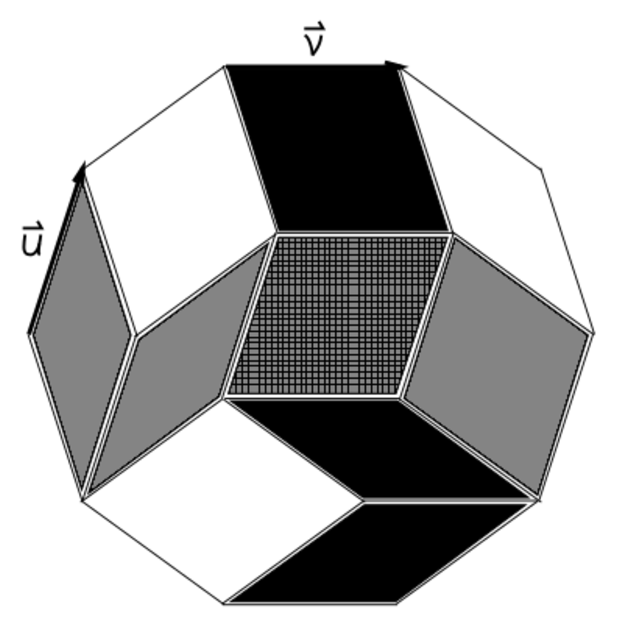
\includegraphics[scale=0.5]{Figs/Geometry/dimers}
\end{figure}

Аналогично определяемый путь для другой стороны $v$ должен пересечь $u$, и их общая плитка, разумеется, образована сторонами $u$ и $v$.
Могут ли они пересечься дважды?
Нет, поскольку при повторном пересечении угол между $u$ и $v$ в их общем ромбе превысил бы $\pi$.\heart

Данная задача досталась мне от Дейны Рэндaлл из Технологическoго института Джорджии.
%(Dana Randall of Georgia Tech).

\subsubsection*{Векторы на многограннике}% (VECTORS ON A POLYHEDRON)

На эту задачу обратил моё внимание Ювал Перес, профессор факультета статистистики Калифорнийского университета в Беркли. %( (Yuval Peres of the Department of Statistics at UC Berkeley).
Самый простой способ понять, что сумма векторов должна быть нулевой --- это провести следующий умственный эксперимент.
Накачаем воздух в (жёсткий) многогранник и отметим, что давление на грань есть сила, действующая по нормали, и её величина пропорциональна площади поверхности грани.
Давление на грани должно быть уравновешено, иначе многогранник бы двигался по собственному усмотрению.
\heart

\subsubsection*{Три окружности}% (THREE CIRCLES)

Эта задача является лучшим известным мне примером эффективности повышения размерности пространства.
Заменим каждую окружность сферой с центром на плоскости, чьё пересечение с плоскостью и есть заданная окружность.
Теперь, каждой паре сфер соответствует конус, и искомые точки являются вершинами трёх конусов. %???забыл про центр

Но все эти вершины лежат на плоскости, которая касается сфер сверху, и точно так
же, они все лежат на плоскости, которая касается сфер снизу.
Значит, oни принадлежат пересечению двух плоскостей --- прямой! \heart

Похоже, что это старинная классическая задача.
Впервые я услышал её от Дейны Рэндaлл, %(Dana Randall), 
из колледжа компьютерных наук Технологическoго института Джорджии.
Вадим Жарницкий, из университета Иллинойса, заметил, что можно задать аналогичный вопрос о четырёх сферах в 3-мерном пространстве: будут ли вершины шести конусов, определяемых данными сферами, лежать на одной плоскости?
Так оно и будет, и один из способов это доказать --- повысить размерность до 4-х.

\subsubsection*{Сфера и четырёхугольник}% (SPHERE AND QUADRIATERAL)

Эту задачу я получил от Тани Ховановой, приглашенного научного сотрудника Принстонского университета в рамках программы по прикладной и вычислительной математике.
У неё есть коллекция задач, которые она зовёт «гробами».
Oна пишет:

\medskip

\begin{trivlist}\leftskip=1cm\rightskip=.5cm
\item\relax«Математико-механический факультет Московского Государственного университета, самая престижная математическая школа России, в своё время (1975) очень активно пытался препятствовать поступлению еврейских (и других „нежелательных“) студентов на факультет.
Один из методов, используемых в этих целях, был таков: неугодным студентам давался на устном экзамене отдельный набор задач.
Задачи эти выбирались очень аккуратно, они имели простое решение (дабы факультет мог избежать скандала), которое было почти невозможно найти.
Любому, кто не решал задачу, могли с лёгкостью отказать в приёме, так что подобная система эффективно контролировала поступление на МехМат.
Такого сорта задачи неформально называли \glqq гробами\grqq.» %???
\end{trivlist}

\medskip

Следующее решение, действительно, найти трудно, но, полагаю, не совсем невозможно.
Сначала следует понять, что для того, чтобы пространственный четырёхугольник оказался плоским достаточно, чтобы его диагонали (или их продолжения) пересекались в некоторой точке.
Заметим, что каждая вершина четырёхугольника $i$ находится на одинаковом расстоянии $d_i$ до точек касания образующих её сторон.
Снабдим вершину $i$ массой $1/d_i$, тогда центр масс двух соседних вершин есть точка касания их общей стороны.
Из этого следует, что центр масс всех четырёх точек лежит на отрезке, соединяющем противоположные точки касания --- это и есть искомая точка.
\heart

\subsubsection*{Восьмёрки на плоскости}% (FIGURES 8S IN THE PLANE)

Эта задача известна уже около 50-ти лет.
Мне говорили, что автором её является великий тополог, профессор университета штата Техас Роберт Ли Мур (1882---1974). %(Robert Lee Moore; 1882—1974).
Читатели, незнакомые с разными степенями «бесконечности», могут уже пребывать в недоумении: ведь очевидно, что на плоскости можно нарисовать бесконечно много восьмёрок, например, поместив по одной восьмёрке внутри каждой клетки квадратной решётки.
О таком множестве мы говорим, что оно счётно. 
Это означает, что восьмёрки можно пронумеровать натуральными числами, так, что каждой восьмёрке будет соответствовать только одно число.

Множество целых чисел, множество всех пар целых чисел, и, таким образом, множество рациональных чисел --- всё это счётные множества, но, как было замечено блестящим (но зачастую депрессивным) математиком Георгом Кантором в 1878 году, множество вещественных чисел не является счётным.
Можно было бы начертить на плоскости концетрические окружности всех возможных положительных вещественных диаметров, и, следовательно, если бы в задаче говорилось об окружностях вместо восьмёрок, ответ был бы «несчётное число», или, более точно, «равномощно множеству вещественных чисел».% (the cardinality of the reals).

Тем не менее, можно нарисовать только счётное число восьмёрок.
Каждой восьмёрке поставим в соответствие пару рациональных точек (точки на плоскости, чьи обе координаты --- рациональные числа), по одной в каждой петле.
Никакие две восьмёрки не могут иметь общих пар точек.
Значит, мощность множества восьмёрок не превышает мощности множества пар из пар рациональных чисел, которое является счётным.\heart

Более хитрую версию данной задачи смотрите в Главе 11 («Крепкие орешки»).

\chapter*{География(!)}
\addcontentsline{toc}{chapter}{География(!)}

\setlength{\epigraphwidth}{.45\textwidth}
\epigraph{Без географии мы были бы нигде.}{---Джимми Баффет (1946---)}%???- или --- 

Да, данная глава не принадлежит этой книге. %(не из этой книги).
Некоторые из задач, представленных здесь, конечно, математические по своей природе, %(mathematical in nature) 
но, в основном, они включены в книгу потому, что доставляют, как мне кажется, большое удовольствие любителям математических головоломок.
Мой издатель уверял меня, что без «Географии» стоимость книги была бы такой же.

Так что эта глава как бы бесплатное приложение, и её можно пропустить с чистой совестью.

Основная тема приведённых ниже задач --- поверхность планеты Земля.
Хотя предпочтение всё-таки отдаётся моей родине --- Соединённым Штатам Америки. 
О чём прошу прощения у читателей из других стран.
Я буду очень благодарен за подобные задачи про разные страны, присланные мне на pw@akpeters.com.

Несколько из этих задач показывают до какой степени %( test the degree) 
картографическая проекция %( на плоскость) (planar projections) 
искажает наше представление о земном шаре. %(глобусе, globe).
Вот одна из них: 

\subsection*{Африка}
\rindex{Африка}

Какой штат США ближе всего к Африке? 

\paragraph{Решение:} Штат Мэн.\heart
  
Он совсем не близко --- проверьте по глобусу.
Но если вы летите по ортодромии (в картографии и навигации ортодромия --- название кратчайшего расстояния между двумя точками на поверхности Земли) из Майами, скажем, в Касабланку, вначале ваш курс %(путь)
будет лежать на Северо-Восток вдоль восточного побережья и пройдёт очень близко к штату Мэн.
%(not missing Maine by much)

\medskip

Дальше попробуйте сами.

\subsection*{На восток от Рино}%EAST OF RENO 
\rindex{На восток от Рино}

Какой самый большой город в США к востоку от Рино, Невада и к западу от Денвера, Колорадо? 

\subsection*{Телефонный звонок}%(THE PHONE CALL) 
\rindex{Телефонный звонок}

Представьте, что вы звоните из какого-то штата Восточного побережья в один из штатов Западного побережья США, и на обеих концах одно и то же время суток.
Как такое может быть? 
  

\subsection*{Диаметр Соединённых штатов}%(THE DIAMETR OF US)  
\rindex{Диаметр Соединённых штатов}

В каких двух штатах находятся две самые удалённые точки США? 
  

\subsection*{На юг от Ки-Уэст}% ( SOUTH FROM KEY-WEST) 
\rindex{На юг от Ки-Уэст}

Если вы летите на юг от города Ки-Уэст, Флорида, какая южно-американская страна вам 
встретится первой? 

\subsection*{Индейцы на среднем западе}% (INDIANS IN THE MIDWEST) 
\rindex{Индейцы на среднем западе}

Среди штатов Среднего Запада США только один имеет название не индейского происхождения? Который?    

\subsection*{Самый большой второй по величине город}% (THE LARGEST SECOND-LARGEST CITY)  
\rindex{Самый большой второй по величине город}

Какой город в США самый большой среди городов с одинаковыми именами, но не больше города США с таким же именем?

\medskip

Эта формулировка может показаться несколько путаной.
Спросим по-другому: скажем, что город (в США) «находится в тени», если существует б\'{о}льший город с таким же именем.
Например, Портланд, штат Мэн, находится в тени города Портланд, штат Орегон.

Итак, наш вопрос прозвучит теперь так: какой наибольший город в США находится в тени?   

\subsection*{Естественные границы}% (THE NATURAL BORDERS) 
\rindex{Естественные границы}

Граница штата может быть естественной (определяться водоёмами, горами и пр.) или 
закреплённой в законе искусственной линией --- в одном знаменитом случае (связанном со штатом Делавэр и Пенсильванией ) --- это дуга окружности.
Три штата --- Колорадо, Юта и Вайоминг имеют только искусственные границы.
Какой штат обладает только естественными границами?   

\subsection*{Непересекаемые границы}% (THE UNCROSSABLE BORDER) 
\rindex{Непересекаемые границы}

Говоря о границах штатов, можете ли вы найти такой штат, который нельзя пересечь на автомобиле? Другими словами укажите два штата, имеющих общую границу, через которую, однако, невозможно напрямую проехать на автомобиле из одного штата в другой?   

\subsection*{Отдел странных названий}% (DEPARTMENT OF ODD NAMES) 
\rindex{Отдел странных названий}

Что особенного в неком местечке, именуемом Уэст-Куодди-Хед, %(West Quoddy Head) 
штат Мэн?   

\subsection*{Городской и деревенский}%(URBAN AND RURAL) 
\rindex{Городской и деревенский}

Данная задача скорее более социологического плана.
В наши дни большинство американцев --- порядка 75\% --- живут в так называемых «городских агломерациях (урбанизированных зонах)».
Перепись населения 2000 года относит к «городскому» 100\% населения одного из штатов и только 27,6\% населения другого штата, который отдалён от первого всего лишь на несколько сот миль.
Можете назвать эти два штата?   

\subsection*{Города на север и на юг}% (CITIES NORTH AND SOUTH) 
\rindex{Города на север и на юг}

Как обстоит дело с вашей визуализацией континентов?
Проверьте, как точно вы представляете себе %(визуаилизируете) 
карту мира.
Расставьте следующие четыре города по порядку с юга на север: 
Галифакс, Новая Шотландия; %(Halifax, Nova Scotia) 
Токио, Япония; %(Tokyo, Japan); 
Венеция, Италия; %(Venice, Italy); 
Алжир, Алжир. %(Algiers, Algeria).

\subsection*{Город в один слог}% (THE ONE-SYLLABLE CITY) 
\rindex{Город в один слог}

Какой город в США, имя которого состоит из одного слога, самый большой? 

\subsection*{Вашингтоны и феминисты}%(WASHINGTONS AND FEMINISTS) 
\rindex{Вашингтоны и феминисты}

Данная задача --- это своеобразный тест на знание не только карты штатов США, но и их английских названий.
Чтобы найти решение этой задачи, вам придётся пользоваться исключительно оригинальными английскими названиями штатов.
Итак, вопрос: 

Сможете ли вы проложить маршрут для автомобиля из города Сиэтл, штат Вашингтон, 
 в Вашингтон, округ Колумбия, таким образом, чтобы названия всех штатов, через которые вы планируете проехать, начинались только с букв, составляющих слово «WOMAN»?
%???добавленно 

\medskip

Наша последняя географическая задача напоминает нам, что пора возвращаться к математике. %(signals us a(slight) return to mathematics) направляет 

\subsection*{Учёный и медведь}%(THE NATURALIST AND THE BEAR) 
\rindex{Учёный и медведь}

Учёная-биолог покинула лагерь экспедиции, прошла 10 миль на юг, затем 10 миль на восток и тут заметила и сфотографировала медведя.
Пройдя 10 миль на север, она пришла обратно в лагерь.

\medskip

Вы не видели фотографии, но всё равно знаете, какого цвета был медведь, не так ли?

%ё
\section*{Решения и комментарии}

Для проверки правильности ответов бы можете воспользоваться атласом, глобусом, альманахом или итогами переписи населения США 2000 года. 
Давайте посмотрим, насколько верны были ваши предположения...
%(догадки)

\subsubsection*{На восток от Рино}% (EAST OF RENO)

Вопрос о самом большом городе может оказаться довольно щекотливым; 
%(awkward question) 
стандартно это понятие определяется количеством населения (не площадью!) в официальных границах города, что, безусловно, может привести к неверным выводам
при наличии городских агломераций.
%(урбанизированных зон)
%(can be misleading with respect to metropolitan area).
Так, например, согласно данным альманаха город Джэксонвилл, штат Флорида, представляется больше, чем Атланта, штат Джорджия, несмотря на то, что население всей городской агломерации Атланты превышает население Джэксонвилла почти в четыре раза.

\medskip

Но в нашей задаче нам не понадобятся такие тонкости. Самый большой город к востоку от Рино и к западу от Денвера, в любом случае, Лос-Анджелес, Калифорния.                                 \heart

\subsubsection*{Телефонный звонок}%ТЕЛЕФОННЫЙ ЗВОНОК (THE PHONE CALL)

«Восточное побережье» Соединённых Штатов Америки включает в себя восточные штаты, имеющие выход к Атлантическому океану, от штата Мэн на севере до штата Флорида на юге. 
К «Западному побережью» относятся штаты Вашингтон, Орегон и Калифорния,
к которым, если хотите, вы можете добавить Аляску и даже Гавайи, но это не так уж важно в данном случае. %(but it doesn’t help).

Обычно, делая подобные звонки, мы имеем разницу во времени между Восточным и Западным побережьем в 3 часа. Мы можем избавиться от одного часа, позвонив из западного района так называемой «ручки ковша» Флориды --- её северо-западной части, % ( Florida panhandle) 
скажем, из города Пенс\'{а}кола, который находится в Центральном часовом поясе. 
Чтобы избавиться ещё от одного часа, мы звоним в один из городов самого восточного района штата Орегон (скажем, Онтарио), в котором Горное время. 

Оставшийся час исчезнет, если звонок будет сделан из Пенсаколы между двумя и тремя часами ночи, при переходе с Летнего времени на Зимнее. 
В этот момент в Центральном часовом поясе время уже переведут на один час назад, а Горное время всё ещё будет прежним.\heart 

       
                                  
\subsubsection*{Диаметр Соединённых штатов}%ДИАМЕТР СОЕДИНЁННЫХ ШТАТОВ (THE DIAMETR OF US) 

Очевидно, это либо Гавайи и Мэн, либо Аляска и Флорида. Или это Гавайи и Аляска?

\medskip

Удивительным образом, ни одно, ни другое, ни третье. Правильный ответ --- Гавайи и Флорида.\heart

\subsubsection*{На юг от Ки-Уэст}%НА ЮГ ОТ КИ-УЭСТ ( SOUTH FROM KEY-WEST)

Это, без сомнения, каверзный вопрос. %(a trick question). 
Вы не пересечёте ни одну страну Южной Америки. 
Ваш путь пройдёт к западу от континента. 
%(Ваш путь пройдёт вдоль западного побережья всего континента.)
\heart

\subsubsection*{Индейцы на среднем западе}%ИНДЕЙЦЫ НА СРЕДНЕМ ЗАПАДЕ (INDIANS IN THE MIDWEST)

По определению к штатам Среднего Запада относятся Миннесота, Висконсин, Айова,
Иллинойс, Миссури, Мичиган, Огайо, Канзас и Небраска --- все названия индейского
происхождения, и остаётся ответ --- Индиана!\heart

Любопытно, что только один штат к востоку от Миссисипи имеет столицу, чьё имя индейского происхождения --- Флорида (Таллахасси).

\subsubsection*{Самый большой второй по величине город}%САМЫЙ БОЛЬШОЙ ВТОРОЙ ПО ВЕЛИЧИНЕ ГОРОД (THE LARGEST SECOND-LARGEST CITY)  

Портланд, штат Мэн? Спрингфилд, Где-нибудь? 
Частые, но не верные предположения.
До 1975 года или около того, правильный ответ был бы Канзас-Сити, штат Канзас, который затеняется городом Канзас-Сити, Миссури.
Затем некоторое время победителем был Колумбус, Джорджия, находящийся в тени столицы Огайо. Однако, мы живём в эпоху пригородов, %(in the age of suburbia), 
перепись населения 2000 года показывает, что теперь городу Глендейл, штат Калифорния (находится в тени Глендейла, Аризона) принадлежит эта сомнительная %(obscure) 
честь.\heart

\subsubsection*{Естественные границы}%ЕСТЕСТВЕННЫЕ ГРАНИЦЫ (THE NATURAL BORDERS)

Конечно, Гавайи имеют только естественные границы. Возможно, вы подумали, что это было слишком легко, но люди часто не видят, что находится у них под носом. 
%(не замечают очевидного) %(folks often have a blind spot).
\heart

\subsubsection*{Непересекаемые границы}%НЕПЕРЕСЕКАЕМЫЕ ГРАНИЦЫ (THE UNCROSSABLE BORDER)

Здесь намного сложнее. Висконсин и Мичиган имеют общую длинную границу по озеру Мичиган, но вы можете пересечь её на пароме Манитовок-Ладингтон, сидя в своей машине. Паром из Монток Пойнт %(Mantauk Point) 
(штат Нью-Йорк) на остров Блок %(Block Island) 
(штат Род-Айленд) пересекает не очень хорошо известную границу между этими двумя штатами, и он только для пассажиров. 
Возможно, существуют и другие решения данной задачи.\heart
                             

Можно задать схожий вопрос о части штата, попасть в которую на автомобиле из остального штата возможно только, проехав через другой штат (или Канаду, в случае с 
Пойнт Робертс). %(Point Roberts). 
Существует несколько таких мест, особенно около вечно меняющейся реки Миссисипи.

\subsubsection*{Отдел странных названий}%ОТДЕЛ СТРАННЫХ НАЗВАНИЙ (DEPARTMENT OF ODD NAMES)

Уэст-Куодди-Хед %(West Quoddy Head) 
--- самая восточная точка континентальных штатов США.\heart
                            

Иногда вам может встретиться утверждение, что, если опустить требование «континентальный», мыс Врангеля %(Cape Wrangel) 
на острове Атту, %(Attu Island) 
штат Аляска, является самой восточной точкой США, но я не принимаю в рассчёт эти «Гринвич-централизованные» доводы. 
%(but I do not buy Greenwich-centered reasoning) 
Назовёте ли вы мыс Врангеля самой восточной точкой Аляски?

\subsubsection*{Городской и деревенский}%ГОРОДСКОЙ И ДЕРЕВЕНСКИЙ (URBAN AND RURAL)

Нью-Джерси и Вермонт. Эту и множество другой интересной информации вы можете найти на сайте:\\
\texttt{http//www.census.gov/prod/2002pubs/01statab/pop.pdf} 
 \heart                          

\subsubsection*{Города на север и на юг}%ГОРОДА НА СЕВЕР И НА ЮГ (CITIES NORTH AND SOUTH)

Токио, Алжир, Галифакс и, наконец, Венеция. Широты, соответственно
$35^\circ 40’$ с.ш.; $36^\circ 50’$ с.ш.; $44^\circ 53’$ с.ш.; и $45^\circ 26’$ с.ш. 
Обратите внимание --- последние два города разделяет 45-я параллель, и это позволяет нам яснее увидеть, что Венеция находится севернее. Один уроженец Новой Шотландии однажды проспорил мне по этому случаю 1 доллар.%по этому случаю???
\heart

\subsubsection*{Город в один слог}%ГОРОД В ОДИН СЛОГ (THE ONE-SYLLABLE CITY)

Йорк, штат Пенсильвания, и Трой, штат Нью-Йорк, называются чаще всего, но всё же Флинт, штат Мичиган, несмотря на существенное сокращение населения за последние годы, остаётся единственным однослоговым городом в США с населением более 100 тысяч человек.
Хотя, если судить по тому, как произносят названия городов местные жители, победителем, несомненно, будет Нью-Арк («Норк», с длинным «о»), штат Нью-Джерси. \heart

\subsubsection*{Вашингтоны и феминисты} %ВАШИНГТОНЫ И ФЕМИНИСТЫ (WASHINGTONS AND FEMINISTS)

Без проблем. Вначале ваш маршрут пойдёт на юг --- через Орегон (Oregon), 
Неваду (Nevada) 
и Аризону, (Arizona), 
затем на восток сквозь Нью-Мексико (New Mexico) 
в Оклахомовскую «ручку ковша», из северо-восточного угла Оклахомы (Oklahoma) 
вы попадаете в Миссури (Missouri). 
Здесь вам надо будет повернуть на север и из северо-западного угла штата проехать в Небраску (Nebraska), продолжая путь на запад в Вайоминг (Wyoming) и на север в Монтану (Montana) --- довольно большой круг для того, чтобы объехать Айдахо (Idaho). 
В конце концов, вы сможете снова развернуться и поехать на восток через Северную Дакоту (North Dakota), 
Миннесоту (Minnesota), 
Висконсин (Wiskonsin) 
и Мичиган (Michigan).
Теперь берите курс на юг в Огайо (Ohio) и на восток сквозь Западную Виргинию (West Virginia) в Мериленд (Maryland),
 и в Вашингтон (Washington DC), округ Колумбия.\heart

Чтобы пройти по этому маршруту, вам придётся несколько раз %(или на долгое время) 
покинуть национальную систему межштатных автомагистралей, но мы предполагаем, вы никуда не торопитесь.

\subsubsection*{Учёный и медведь}%УЧЕНЫЙ И МЕДВЕДЬ (THE NATURALIST AND THE BEAR)

Начальная идея была, конечно, что лагерь экспедиции находился на Северном полюсе, так как маршрут учёной (10 миль на юг, 10 миль на восток и 10 миль на север) является замкнутым контуром, %(to have been a closed loop), 
следовательно медведь был белый.

Однако, как было замечено в одной из рубрик %(колонок) 
Мартина Гарднера, %(Martin Gardner’s columns), 
на поверхности Земли существует бесконечно много других точек, где подобный путь будет замкнутым.

Некоторые из этих точек лежат на окружности с центром в Южном полюсе и радиусом немного меньше $10 + \tfrac5\pi$ миль.
Начав прогулку с такой точки, наша учёная после первых 10 миль окажется в некой точке $P$, 
находящейся на расстоянии чуть меньше $\tfrac5\pi$ миль от Южного полюса. 
Повернув на Восток и пройдя 10 миль, она обогнёт весь мир и вернётся в точку $P$, откуда 10 миль на Север приведут её обратно в лагерь.

Другая окружность, радиусом чуть меньше $10 + \tfrac5{2\pi}$ миль тоже сработает, во второй (Восточной) части пути наша учёная должна будет 2 раза обойти вокруг Южного полюса и так далее.

В Антарктике медведи не водятся, но если бы водились, то, наверное, были бы белыми.
Так что ответ задачи не изменится.\heart

\chapter*{Игры}
\addcontentsline{toc}{chapter}{Игры}

\setlength{\epigraphwidth}{.6\textwidth}
\epigraph{Деньги никогда не были для меня серьёзной мотивацией, это просто способ считать очки.
Настоящий азарт --- вести игру.}{---Дональд Трамп (1946---).
«Трамп: Искусство сделки»}
%Сами по себе деньги меня не интересуют, это только способ считать очки. Азарт в самой игре.  
%(Деньги никогда не были для меня серьёзной мотивацией – скорее способом вести счёт. Настоящее возбуждение получаешь от процесса игры)

Иногда  описание игры приводит к чудесной задаче.
А честная ли игра? А какова наилучшая стратегия? Особенность этой главы состоит в том, что каждая задача имеет две версии, различия между которыми весьма занимательны.
Здесь представлены четыре пары игр: в первой паре речь пойдёт о числах, во второй --- о шляпах, в третьей --- о картах, и в четвёртой --- о гладиаторах.

\medskip

Начнём с классической игры, являющейся  хорошим примером класса вероятностных алгоритмов (и действительно, она так и использовалась Мануэлем Блюмом,  профессором университета Карнеги --- Меллона). %(Manuel Blum from  Carnegie Mellon University)

\subsection*{Сравнение чисел, версия I} % (COMPARING NUMBERS, VERSION I)
\rindex{Сравнение чисел, версия I}

Паула (злоумышленник) пишет на двух листочках бумаги по целому числу.
На числа нет никаких ограничений, кроме того, что они должны быть различными.
Она прячет в каждой руке по бумажке.

Виктор (жертва) выбирает руку Паулы, которую она открывает и показывает число на листочке бумаги.
Виктор теперь должен угадать, является ли это число б\'{о}льшим или меньшим из двух чисел Паулы.
Если он угадывает правильно, он выигрывает 1 доллар, если нет --- проигрывает 1 доллар.

Очевидно, Виктор может обеспечить себе равные шансы в игре, подбрасывая, например, монету, чтобы выбрать между «большее» и «меньшее».
Вопрос: не зная ничего о характере Паулы, может ли Виктор сыграть лучше, чем просто остаться при своих?

\subsection*{Сравнение чисел, версия II} %(COMPARING NUMBERS, VERSION II)
\rindex{Сравнение чисел, версия II}

Давайте теперь упростим Виктору задачу:
Паула не загадывает больше числа, они выбираются независимо случайным образом из интервала $[0,1]$ с равномерным распределением (подойдут два числа, выданные стандартным генератором случайных чисел).

Чтобы не обижать Паулу, позволим ей проверять эти два случайных числа и выбирать, \emph{которое из них показать Виктору}. %???подсмотреть и выбрать какое
И снова, на кону 1 доллар, и Виктор должен решить, является ли это число б\'{о}льшим или меньшим из двух чисел.
Сможет ли Виктор сыграть лучше, чем просто остаться при своих?
Какие у Виктора и Паулы есть лучшие (то есть «равновесные») стратегии?

\subsection*{Синие и красные шляпы, версия I} % (RED AND BLUE HATS, VERSION I)
\rindex{Синие и красные шляпы, версия I}

На каждого члена команды из $n$ игроков надета красная или синяя шляпа.
Каждый игрок видит, какого цвета шляпа у его товарищей, но на свою шляпу он посмотреть не может.
Обмениваться информацией запрещено.
По сигналу все игроки одновременно должны назвать цвет своей шляпы.
После этого те игроки, которые угадали неправильно,  отправляются на казнь.

Зная, что придётся играть, у команды есть возможность договориться о стратегии
(то есть установить набор правил, необязательно одинаковых для всех игроков, какому игроку какой цвет называть, основываясь на том, что он видит).
Их задача --- гарантировать максимально возможное число выживших, предполагая наихудший вариант распределения шляп.

\medskip

Другими словами, допустим, распределяющий шляпы противник знает о командной стратегии и будет стараться всеми силами её расстроить.
Сколько игроков можно спасти?


\subsection*{Синие и красные шляпы, версия II} % (RED AND BLUE HATS, VERSION II)
\rindex{Синие и красные шляпы, версия II}

И снова, на каждого из $n$ игроков команды надевается красная или синяя шляпа.
Но в этот раз игроки выстраиваются в шеренгу по одному, так что каждый игрок видит только шляпы впереди стоящих.
И снова, каждый игрок должен угадать цвет своей шляпы, и  если ошибётся, то будет казнён.
Но в этот раз игроки отвечают по очереди, начиная с конца шеренги.
Таким образом, $i$-тый в шеренге игрок, например, видит какого цвета шляпы у $1, 2,\dots, i-1$ игрока и слышит, что сказали $n, n-1,\dots, i+1$ игроки.
(При этом он не знает, какие из ответов правильные --- казнь состоится позже).

\medskip

Как и прежде, у команды есть возможность договориться заранее о стратегии, которая бы гарантировала им максимально возможное число выживших.
При наихудшем раскладе, сколько игроков можно спасти?

\subsection*{Ставка на следующую карту, версия I} % (BETTING ON THE NEXT CARD, VERSION I)
\rindex{Ставка на следующую карту, версия I}

Паула тщательно тасует колоду карт, затем открывает по одной карте, снимая карту с верха колоды.
В любой момент Виктор может прервать её и поставить 1 доллар на то, что следующая карта будет красной.
Он делает ставку ровно один раз.
Если он ни разу не останавливает Паулу, то ставка автоматически делается на последнюю карту.

\medskip

Какова лучшая для Виктора стратегия?
Насколько его шансы лучше, чем 50/50? 
(Предполагается, в колоде 26 красных и 26 чёрных карт.)

\subsection*{Ставка на следующую карту, версия II} % (BETTING ON THE NEXT CARD, VERSION II)
\rindex{Ставка на следующую карту, версия II}

И снова, Паула тщательно тасует колоду и затем открывает по одной карте.
Виктор начинает играть, имея в наличии один доллар.
Он может поставить  любую часть имеющейся у него на данный момент суммы на цвет следующей карты.
Его шансы на выигрыш не зависят от текущего состава колоды.
Так, например, он может отказываться делать ставки до последней карты, чей цвет он, понятно, будет знать, уверенно поставить всё и уйти домой с двумя долларами.

\medskip

Существует ли стратегия, которая может \emph{гарантировать} Виктору закончить игру с суммой больше, чем 2 доллара?
Если да, какую максимальную сумму он может гарантированно выиграть? 

\subsection*{Гладиаторы, версия I} % (GLADIATORS, VERSION I)
\rindex{Гладиаторы, версия I}

У Паулы и Виктора есть по команде гладиаторов.
Гладиаторы Паулы обладают силой $p_1, p_2,\dots, p_m$, а гладиаторы Виктора --- $v_1, v_2,\dots, v_n$.
Гладиаторы бьются до смерти один на один, и когда гладиатор силы $x$ встречается с гладиатором силы $y$, первый побеждает с вероятностью $x/(x+y)$, а второй с вероятностью $y/(x+y)$.
Более того, если гладиатор силы $x$ побеждает, то он обретает уверенность и наследует силу противника, так что его сила увеличивается до $x+y$.
Аналогично, если побеждает второй гладиатор, его сила увеличивается с $y$ до $x+y$.

После каждого поединка Паула выставляет на ринг гладиатора (из тех в её команде, кто ещё остался в живых), и Виктор должен выбрать одного из своих гладиаторов для поединка.
Выигрывает та команда, в которой остаётся хотя бы один живой боец.

\medskip

Какова наилучшая стратегия для Виктора?
Например, если Паула начинает с её лучшего гладиатора, должен ли в ответ Виктор выставить сильного или слабого?

\subsection*{Гладиаторы, версия II} % (GLADIATORS, VERSION II)
\rindex{Гладиаторы, версия II}

И снова, Паула и Виктор должны противостоять друг другу в Колизее, но на этот раз сила не меняется --- когда гладиатор побеждает, его сила остаётся той же, что была.

\medskip

Как и прежде, перед каждым поединком Паула выбирает участника первой.
Какова лучшая для Виктора стратегия? Кого он должен выставить на бой, если Паула начинает с лучшего бойца?

\section*{Решения и комментарии}

\subsubsection*{Сравнение чисел, версия I}% (COMPARING NUMBERS, VERSION I)

Насколько мне известно, данная задача была придумана Томом Ковером %(Tom Cover) 
в 1986 году.%
\footnote{T. Cover, ``Pick the largest number''. \emph{Open problems in communication and computation.} Springer, (1987) p. 152.}
Удивительным образом, существует стратегия, гарантирующая Виктору победу с вероятностью больше $50\%$.

\medskip

До начала игры Виктор должен обзавестись вероятностным распределением на множестве целых чисел таким, что каждому целому числу назначается положительная вероятность.
(Например, он может подбрасывать монету до первой решки.
Если выпадает чётное число $2k$ орлов, то он выбирает целое число $k$, если выпадет $2k-1$ орлов, ему нужно выбрать целое число $-k$.)

Если Виктор умён, он скроет это распределение от Паулы, но, как вы увидите позже, у Виктора всё равно будет гарантия победы, даже если Паула узнает его секрет.

После того, как Паула записала свои числа, Виктор выбирает целое число из его вероятностного распределения и прибавляет к нему $\tfrac12$, полученную величину  $t$ назовём «порогом».
Например, используя распределение выше, если вышло $5$ орлов до первой решки, то его случайное целое число будет $-3$, и порог $t$ будет равен~$-2 \tfrac12$.

Когда Паула начинает игру, Виктор подбрасывает монету, чтобы решить какую руку выбрать, потом смотрит на число в этой руке.
Если число превышает $t$, он полагает, что это большее из чисел Паулы, если оно меньше, чем $t$, то считает, что оно меньшее.

А почему это работает? 
Предположим, $t$ оказывается больше, чем оба числа Паулы.
Тогда ответ Виктора будет «меньшее», независимо от того, какое число ему достанется, и, таким образом, шанс угадать равен $\tfrac12$.
Если $t$ меньше обоих чисел Паулы, Виктор, несомненно, скажет «большее», и, опять, вероятность выигрыша будет равна $\tfrac12$.

Но, \emph{с положительной вероятностью}, порог $t$ может оказаться между двумя числами Паулы, и тогда Виктор выигрывает вне зависимости от того, какую руку он выбрал.
Эта возможность, и обеспечивает вероятность выигрыша более $50\%$.\heart

Ни эта, ни какая-либо другая стратегия не даёт Виктору гарантию, что при некотором фиксированном $\varepsilon>0$ вероятность выигрыша превысит $50\%+\varepsilon$.
Умная Паула может выбрать два последовательных многозначных целых числа, и тем самым, свести преимущество Виктора к самой малости.

\subsubsection*{Сравнение чисел, версия II}% (COMPARING NUMBERS, VERSION II)

Может показаться, что возможность решать, которое число увидит Виктор, является для Паулы ничтожной компенсацией того, что не она выбирает числа.
Но, на самом деле, \emph{эта} версия игры абсолютно честная:
Паула может исключить какое-либо преимущество Виктора в игре.

У неё простая стратегия --- посмотреть на два случайных вещественных числа, затем скормить Виктору то, что ближе к~$\tfrac12$.

Это приводит Виктора к чистому угадыванию.
Чтобы это понять, предположим, что число $x$, показанное ему, лежит между $0$ и $\tfrac12$.
Тогда скрытое число равномерно распределено на множестве $[0,x]\cup [1-x, 1]$, и, таким образом, с одинаковой вероятностью будет больше или меньше $x$.
Если $x>\tfrac12$, то рассматривается множество $[0, 1-x]\cup [x, 1]$, и далее рассуждение аналогично.

Конечно, Виктор может гарантировать вероятность $\tfrac12$ при любой стратегии, игнорируя само число и подбрасывая монету, так что игра абсолютно честная.
\heart

Эта замечательная игра привлекла моё внимание в ресторане в Атланте.
За столом было много умных людей и все они оказались в тупике.
Так что, если у вас не получилось найти хорошую стратегию для Паулы, то вы оказались в хорошей компании.

\subsubsection*{Синие и красные шляпы, версия I}% (RED AND BLUE HATS, VERSION I)

Не сразу очевидно, что хоть кого-то можно спасти.
Часто первой рассматривают стратегию «большинства»;
то есть, если $n\z=10$, то каждый игрок называет цвет, который он видит на пяти или более из девяти товарищей.
Но это приведёт к десяти казням, если шляпы распределены пять на пять, и наиболее очевидная модификация этой схемы при наихудшем раскладе также закончится кровавой бойней.

\medskip

Тем не менее, легко спасти $[n/2]$ игроков с помощью следующего приёма.
Игрокам надо разбиться на пары (скажем, муж и жена), каждый муж выбирает цвет шляпы жены, и каждая жена выбирает цвет, \emph{противоположный} цвету шляпы её мужа.
Очевидно, если у пары шляпы одного цвета, муж останется в живых, если нет, выживет жена.

Чтобы понять, что это наилучший возможный вариант, представим, что цвета распределяются не противником, а равномерно случайным образом (например, подкидывая монету).
Независимо от стратегии, вероятность того, что какой-либо конкретный игрок выживет, равна $\tfrac12$.
Значит, матожидание числа выживших равно $n/2$. 
Из этого следует, что \emph{минимальное} число выживших не может превысить $[n/2]$.\heart

\subsubsection*{Синие и красные шляпы, версия II}% (RED AND BLUE HATS, VERSION II)

Эту версию про красные и синие шляпы мне рассказала Гириджа Нарликар из лабораторий Белла, %(Girija Narliar of Bell Labs)
она услышала её на одной вечеринке (предыдущая версия --- мой ответ на задачу Гиринджи, хотя, несомненно, она была известна прежде).
В версии с шеренгой легко увидеть, что можно спасти $[n/2]$ игроков.
Например, игроки $n, n-2, n-4,\dots$
могут назвать цвет шляпы товарища, стоящего прямо перед ним, так что игроки $n-1, n-3,n-5,\dots$
повторяют предыдущий ответ и спасаются.

\medskip

Кажется, что вероятностное решение, как и в версии с одновременным угадыванием, должно сработать и здесь, то есть показать, что $[n/2]$ --- максимальное возможное число спасённых игроков.
Вовсе нет --- можно спасти всех игроков, кроме последнего!

Последний в шеренге игрок (несчастный бедолага!) просто говорит:
«Красная», если он видит нечётное число красных шляп впереди себя, в противном случае говорит: «Синяя».
Игрок с номером $n-1$ сможет отгадать, какого цвета на нём шляпа.
Например, если он услышал, что игрок $n$ сказал:
«Красная» и видит \emph{чётное} число красных шляп впереди себя, то он знает, что на нём красная шляпа.

Таким же образом рассуждает каждый последующий в очереди игрок.
Игрок под номером $i$ суммирует число красных шляп,которые он видит, и число услышанных «красных» ответов.
Если это нечётное число, он говорит «Красная», если чётное --- «Синяя», и угадывает правильно (если только кто-то не напортачил).

Конечно же, последнего игрока нельзя спасти, так что $n-1$ --- наилучший возможный вариант.
\heart

Стоит отметить (спасибо Джо Булеру %(Joe Buhler)
за напоминание), что даже при наличии $k$ различных цветов шляп вместо двух, только последний в шеренге игрок приносится в жертву(отправится на казнь).
Он кодирует цвета как $0, 1, 2, \dots, k-1$ и суммирует все цвета шляп, которые он видит, по модулю $k$.
Затем он объявляет цвет соответственно полученной сумме, и теперь каждый последующий игрок может определить цвет своей шляпы, вычитая из заявленного первым цвета сумму цветов, которые он видит, и цветов, названных предыдущими игроками.

Стратегия последнего игрока (при $k=10$) возможно используется вашим банком для генерирования последней цифры номера банковского счёта.

\subsubsection*{Ставка на следующую карту, версия I}% (BETTING ON THE NEXT CARD, VERSION I)

Похоже, что Виктор может добиться небольшого преимущества, дождавшись момента, когда в колоде останется больше красных карт, чем чёрных, и тогда сделать ставку.
Конечно, этого может никогда и не случиться, и если так, Виктор проигрывает.
Компенсируется ли это гораздо большей вероятностью получения малого преимущества?

В действительности, это честная игра.
У Виктора не только нет способа добиться какого-либо преимущества, у него нет и возможности его потерять.
Все стратегии равно неэффективны.

Этот факт является следствием теоремы Дуба об остановке %(of the martingale stopping time theorem) 
и может быть легко доказан индукцией по числу карт каждого цвета в колоде.
Но существует другое доказательство, которое я приведу ниже, и которое, без сомнения, содержится в «Книге».\footnote{Как известно многим читателям, великий, ныне покойный, математик Пал Эрдёш часто говорил о Книге, имеющейся у Бога, в которой записаны лучшие доказательства для всех теорем.
Я представляю себе, что Эрдёш с великим удовольствием читает сейчас эту книгу, но нам придётся ещё подождать.}

Предположим, Виктор выбрал некую стратегию $S$.
Применим $S$ к несколько модифицированной версии этой задачи.
В новом варианте Виктор прерывает Паулу как и прежде, но на этот раз он делает ставку не на \emph{следующую} карту, а на \emph{последнюю} карту в колоде.

Разумеется, в любой ситуации у последней карты точно такая же вероятность оказаться красной, как и у следующей карты в колоде.
Таким образом, стратегия $S$ имеет в новой игре такое же матожидание, как и в предыдущей.

И, конечно же, проницательный читатель уже заметил, что новый вариант игры довольно неинтересен.
Виктор выигрывает, если последняя карта --- красная, независимо от стратегии.
\heart

В книге Т. Ковера и Дж.Томаса% «Элементы теории информации»
\footnote{T. Cover and J. Thomas, \emph{Elements of Information Theory,} Wiley (1991).} 
эта игра обсуждается на основе результата статьи Т. Ковера.%
\footnote{T. Cover, ``Universal Gambling Schemes and Complexity Measures of Kolmogorov and Chaitin''. \emph{Statistics Department Technical Report \#12}, Stanford University, October 1974.}

Модифицированная версия игры %«Следующая карта --- красная»
напоминает об игре, которая много лет назад была описана --- в сатирических целях --- в журнале «Гарвардский пасквилянт».\footnote{Harvard Lampoon Vol. CLVII, No. 1, March 30, 1967, 14--15.
Номер журнала называется «Games People Play Number», и авторами рассматриваемой игры являются, по всей видимости, Д. Кенни и Д. Макклелланд.%(D.C. Kenney and D.C.K. McClelland).
}
Называлась она «Великая игра во искупление и отпущение грехов».
По правилам игроки делают ходы, бросая кубик, и двигаются по круговому полю, похожему на поле «Монополии», пока каждый из них не оказывается на клетке с надписью «Смерть».
Так кто же выигрывает?

В начале игры всем раздаётся по одной карте из «Колоды Судьбы», рубашками вверх.
В конце игры карты открываются, и те, у кого карта «Проклят», проигрывают.

\subsubsection*{Ставка на следующую карту, версия II}% (BETTING ON THE NEXT CARD, VERSION II)

Наконец-то Виктору досталась действительно хорошая игра.
Но может ли он гарантированно сыграть лучше, чем просто удвоить свои деньги, вне зависимости от того, как распределены карты?

\medskip

Для начала полезно будет подумать, какие же из стратегий Виктора будут оптимальными в смысле «матожидания».
Легко увидеть, что как только в колоде остаются карты одного цвета, Виктор должен ставить всё на каждом ходу до конца игры.
Назовём стратегию, которая следует этому правилу, «разумной».
Ясно, что каждая оптимальная стратегия является разумной.

Поразительно, но обратное также верно.
Не важно, какая у Виктора будет стратегия, матожидание будет тем же, при условии, что он будет действовать правильно, когда в колоде останутся карты одного цвета.
Чтобы увидеть это, рассмотрим вначале следующую \emph{чистую} стратегию: Виктор представляет себе какое-то конкретное фиксированное распределение красных и чёрных карт в колоде, и ставит \emph{всё, что у него есть,} согласно этому распределению \emph{на каждую карту}.

Конечно же, с такой стратегией Виктор почти всегда проигрывает, но если он выиграет, то он сможет купить весь Земной шар --- он унесёт домой $2^{52}$ долларов, то есть около 50 квадрильонов.
Поскольку существуют $\binom{52}{26}$ способов распределения цвета карт в колоде, матожидание выигрыша Виктора равно $2^{52}/\binom{52}{26} \approx 9{,}0813$.

Разумеется, эта стратегия не реалистична, но, согласно нашему определению, она «разумна», и, что особенно важно, \emph{каждая разумная стратегия является комбинацией чистых стратегий подобного типа}.
Чтобы это понять, вообразите себе, что у Виктора есть $\binom{52}{26}$ аспирантов, играющих для него, и каждый применяет свою (отличную от других) из чистых стратегий.

Мы утверждаем, что каждая разумная стратегия Виктора сводится к распределению неким образом его первоначальной суммы в 1 доллар среди этих помощников.
Если в какой-то момент его помощники ставят $x$ долларов на красную и $y$ долларов на чёрную карту, то это равносильно тому, что Виктор сам ставит $x-y$ (если $x > y$) на красную карту и $y-x$ на чёрную (при $y>x$).

Каждая разумная стратегия даёт некое распределение следующим образом.
Скажем, Виктор хочет поставить $0{,}08$ долларов на то, что первая карта будет красной.
Это означает, что его помощники, которые первую ставку делают на красное, получают $0{,}54$, в то время, как те, что ставят на чёрную, получают только $0{,}46$.
Если, выиграв, Виктор планирует поставить на следующем ходу $0{,}04$ на чёрную, он выделяет на $0{,}04$ больше помощникам со ставками «красная-чёрная», чем «красная-красная».
Продолжая таким образом, каждый помощник в итоге получит положенную ему сумму денег.

Теперь заметим, любая выпуклая комбинация стратегий с одинаковым матожиданием имеет то же матожидание.
Отсюда следует, что каждая разумная стратегия для Виктора имеет одно и то же матожидание выигрыша в $9{,}08$ (дающий ожидаемую прибыль в $8{,}08$ долларов).
В частности, все разумные стратегии оптимальны.

Но одна из этих стратегий \emph{гарантирует} $9{,}08$ долларов, а именно та, в которой ставка в 1 доллар поровну делится между помощниками.
Поскольку нельзя гарантировать больше, чем матожидание, эта стратегия является наилучшей возможной.\heart

На самом деле, данную стратегию достаточно легко реализовать (предполагая, как и раньше, что валюту США можно делить до бесконечности).
Если в колоде остаётся $b$ чёрных и $r$ красных карт, где $b\ge r$, то Виктор ставит $(b - r)/(b + r)$ от имеющейся у него на данный момент суммы на чёрную; если $r > b$, он ставит $(r - b)/(b + r)$ часть его денег на красную.

\medskip

Если изначальный доллар \emph{не} делится до бесконечности, а состоит из 100 неделимых центов, то ситуация усложняется.
В этом случае Виктор теряет около доллара.
Динамическая программа (написанная Иоаной Димитриу %(Ioana Dimitriu) 
из Калифорнийского университета в Беркли) демонстрирует, что при оптимальной игре, Виктор завершает игру с $8{,}08$ долларами.
Таблица ниже показывает, сколько у Виктора центов на каждой стадии правильно ведущейся игры.
\begin{figure}[h!]
\centering
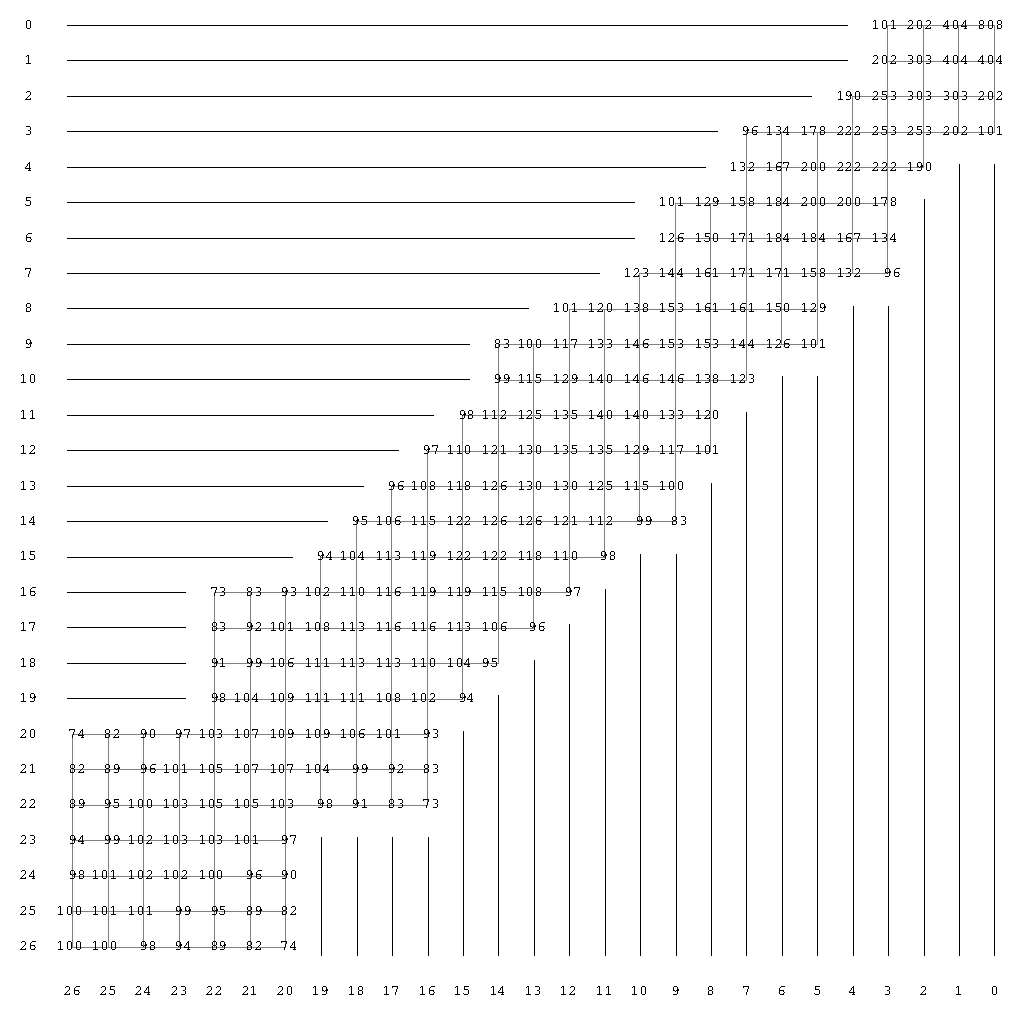
\includegraphics[scale=0.63]{Figs/Games/ioana}
\end{figure}
Например, к моменту игры, когда в колоде остаётся 12 чёрных и 10 красных карт, у Виктора должно быть $129$ центов. 
Сравнивая с числами сверху и справа, мы видим, что он должен поставить либо $11$ центов (в этом случае Паула позволяет ему выиграть) или $12$ центов (в этом случае он проиграет) на то, что следующая карта --- чёрная.

Заметьте, что в 100-центовом варианте игры Виктор делает ставки осторожней, чем в непрерывной её версии.
Если же он решит ставить каждый раз число центов, ближайшее к $(b - r)/(b + r)$ суммы его денег, то Паула разорит его ещё до того, как выйдет половина колоды!

\medskip

Я услышал эту задачу от Раса Лайонса из университета Индианы, %(Russ Lyons, of Indiana University), 
который услышал её от Ювала Переса, %(Yuval Peres), 
который услышал её от Сёрджу Харта. % (Sergiu Hart).
Сёрджу Харт не помнит, где он её услышал, но подозревает, что, скорее всего, Мартин Гарднер писал о ней десятилетия тому назад.

\subsubsection*{Гладиаторы, версия I}% (GLADIATORS, VERSION I)

Как и в первой версии «Ставки на следующую карту», все стратегии для Виктора одинаково хороши.

Чтобы это увидеть, представим себе, что сила гладиаторов --- это деньги.
Паула начинает игру с суммой в $P = p_1 + p_2 + \dots + p_m$ долларов, 
а Виктор с $V = v_1 + v_2 + \dots + v_n$.
Когда гладиатор силы $x$ побеждает гладиатора силы $y$, команда первого гладиатора получает $y$ долларов, в то время, как команда второго теряет $y$ долларов.
Общее количество денег всегда остаётся одним и тем же.
В итоге, либо Паула закончит игру с $P+V$ долларами, а Виктор с $0$ долларов, либо наоборот.

Ключевое наблюдение здесь состоит в том, что каждый поединок --- честная игра.
Если Виктор выставляет гладиатора силы $x$ против гладиатора силы $y$, то ожидаемая прибыль составит 
\[\frac{x}{x+y}y + \frac{y}{x+y}(-x) =0.\]

Таким образом, весь турнир --- честная игра, из чего следует, что для Виктора ожидаемый выигрыш по окончанию игры равен той сумме, с которой он начинал, $V$.
Значит
\[q(P + V) + (1-q)(0) = V,\]
где $q$ --- вероятность того, что Виктор выигрывает.
Таким образом, $q = V/(P+V)$,
независимо от чьей-либо стратегии в турнире.
\heart

Вот ещё одно, более комбинаторное доказательство, придуманное одним из моих любимых соавторов, Грэмом Брайтвеллом, из Лондонской школы экономики. %(Graham Brightwell of London School of Economics).

Применяя приближение рациональными числами и избавляясь от знаменателей, можно предположить, что силы гладиаторов выражаются целыми числами.
Каждому гладиатору припишем $x$ шаров, если его начальная сила равнялась $x$, и расположим все шары равномерно случайным образом в вертикальном порядке.
Когда два гладиатора сражаются, тот, чей шар расположен выше, побеждает (это случается с требуемой вероятностью $x/(x+y)$), и шары проигравшего достаются победителю.

Новый набор шаров выжившего гладиатора имеет такое же однородное вероятностное распределение в начальном вертикальном порядке, как если бы он только что начал игру с полным набором шаров.
Отсюда следует, что результат каждого поединка не зависит от предыдущих событий, что и требовалось доказать.
Вне зависимости от стратегии, Виктор выигрывает тогда, и только тогда, когда самый верхний из всех шаров принадлежит ему.
Это случается с вероятностью $V/(P+V)$.

\subsubsection*{Гладиаторы, версия II}% (GLADIATORS, VERSION II)

Очевидно, что изменение правил приводит к совершенно отличным от предыдущей версии стратегическим соображениям в игре, не так ли? Нет, опять стратегии не имеют значения!

\medskip

Для этой игры, мы отберём деньги (и шары) у каждого гладиатора, и превратим его
в электрическую лампочку.

Для математика идеальная лампочка обладает следующим свойством: её время горения не имеет памяти.
Это означает, что знание того, как долго лампочка горела, абсолютно ничего нам не говорит о том, сколько времени она будет ещё гореть.

Вы, возможно, знаете, что единственное вероятностное распределение, обладающее таким свойством, --- экспоненциальное.
Если ожидаемая (средняя) продолжительность жизни лампочки равна $x$, тогда вероятность того, что она всё ещё горит в момент времени $t$, будет равна $e^{-t/x}$.
Хотя, для данной задачи нам не нужны формулы.
Необходимо только знать, что существует вероятностное распределение без памяти.

Даны две лампочки со средней продолжительностью жизни $x$ и $y$ соответственно.
Вероятность того, что первая будет гореть дольше второй, равна $x/(x+y)$.
Чтобы увидеть это, не применяя матанализ, предположим, что у нас имеется один светильник, который использует только лампочки типа «$x$», и другой, использующий только лампочки типа «$y$».
Каждый раз, когда лампочка перегорает, мы заменяем её на другую такого же типа.
Когда лампочка перегорает, вероятность того, что это $y$-лампочка, является константой, не зависящей от прошлого.
Но эта константа должна быть равной $x/(x+y)$, потому что за долгий промежуток времени $y$-лампочки и $x$-лампочки будут использованы в пропорции $x : y$.

Вернёмся в Колизей.
Представим себе, что поединок двух гладиаторов соответствует включению соответствующих им лампочек.
Они горят до тех пор, пока один из них (проигравший) не перегорает, затем победителя выключают до следующего боя.
Так как распределение не имеет памяти, сила победителя в следующем поединке не изменяется.
Замена гладиаторов лампочками может и не совсем удовлетворяет зрителей, зато является действенной моделью для сражений.

На протяжении турнира у Паулы и Виктора горит ровно по одной лампочке в любой момент времени.
Победителем является тот, чьё общее время горения (всех лампочек/гладиаторов в её/его команде) больше.
Поскольку это не имеет ничего общего с порядком, в котором включались лампочки, вероятность победы Виктора не зависит от стратегии.
(Заметим, эта вероятность --- более сложная функция от сил гладиаторов, чем в предыдущей игре.)
\heart

Игра, где сила постоянна, приводится в статье Каминского, Лакса и Нельсона.%
\footnote{K. S. Kaminsky, E. M. Luks, and P. I. Nelson, ``Strategy, Nontransitive Dominance and the Exponential Distribution''. \emph{Austral. J. Statist.}, Vol.~26, No.~2 (1984), 111--118.}
У меня есть теория, как появилась другая игра: кому-то очень понравилась эта задача и он запомнил ответ (все стратегии одинаково хороши), но не условие.
И когда он или она пытался воссоздать правила игры, то было совершенно естественно ввести условие наследования силы, чтобы получился мартингал.

\chapter*{Алгоритмы}
\addcontentsline{toc}{chapter}{Алгоритмы}

%Achievement is largely the product of steadily raising one’s level of aspiration and expectation.
%Jack Nicklaus (1940 --) “My Story”

\setlength{\epigraphwidth}{.7\textwidth}
\epigraph{Успех в значительной степени является результатом неуклонного роста наших устремлений и ожиданий.}{---Джек Никлаус (1940---) «Моя история»}


%\epigraph{По большей части успех есть результат неуклонного повышения уровня запросов и надежд.}{---Джек Никлаус (1940---) «Моя история»}

Громадное множество очаровательных математических задач закручено вокруг алгоритмов.
Обычно вам (жертвам) предлагается некая ситуация вместе с набором возможных операций и целевое состояние.
Вы можете или не можете выбирать, как применять эти операции.
Вас спросят «Возможно ли достичь целевого состояния?» или, например, «Возможно ли \emph{избежать} целевого состояния?» или, иногда, «А за сколько шагов?».

Как правило, при выполнении операции какой-то аспект меняется в лучшую сторону, но при этом, возможно, что-то портится в другом месте.
Как определить, что цель достижима?

Наша вводная задача была предложена на первой Всероссийской математической олимпиаде 1961 года.

\subsection*{Знаки в таблице}% (SIGNS IN AN ARRAY)
\rindex{Знаки в таблице}

Пусть дана таблица $m\times n$, в клетки которой вписаны вещественные числа, и разрешается одновременно менять знак у всех чисел некоторой строки или некоторого столбца.
Докажите, что можно поменять знаки таким образом, что суммы чисел, стоящих в любой строке и любом столбце, станут неотрицательны.

\paragraph{Решение:}
Поменяв знаки в строке с отрицательной суммой, мы выправим данную сумму, но, возможно, испортим сумму в каком-то столбце.
Как же можно убедиться, что мы улучшили позицию?

Данная задача соответствует первому из следующих классических типов задач.
В задачах на алгоритмы обычно предлагается начальное положение, целевое положение и набор операций, которые можно использовать, чтобы улучшить ситуацию.
Требуется доказать одно из следующих утверждений (но необязательно говорят, которое):
\begin{figure}
\centering
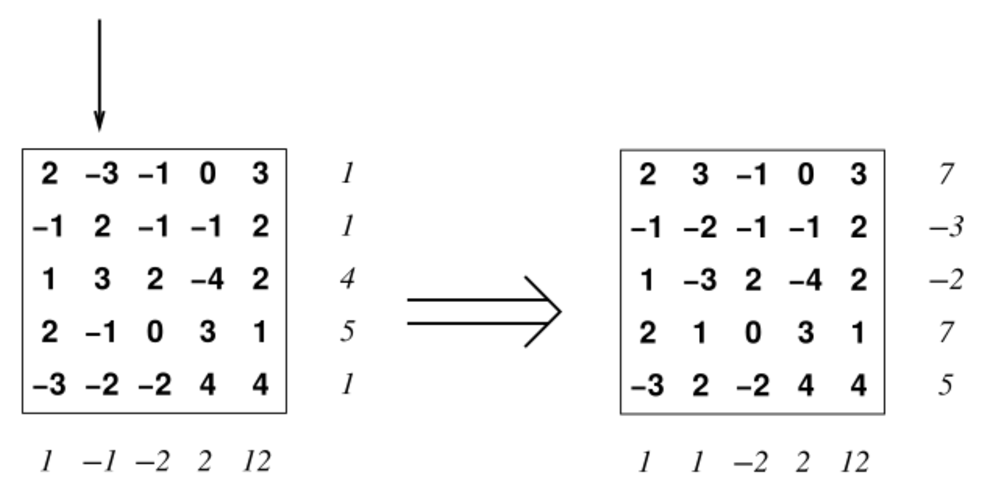
\includegraphics[scale=0.6]{Figs/Algorithms/array}
\end{figure}
\begin{enumerate}[(1)]
\item Существует (конечная) последовательность операций, которая приведёт к целевому положению.
\item Любая последовательность операций в конечном итоге достигнет целевого положения.
\item Каждая последовательность операций достигает цели за одинаковое число шагов.
\item Никакая последовательность операций не может достичь цели.
\end{enumerate}

Алгоритмические задачи обычно решаются нахождением параметра $P$ --- некоего числового показателя состояний, который каким-либо образом закрепляет прогресс продвижения к целевому состоянию.

Для доказательства (1) нужно показать, что до того, как вы достигнете целевого состояния, всегда будет существовать операция (или последовательность операций), улучшающая $P$.
Чтобы не попасть в ловушку парадокса Зенона (делая шаги всё меньше и меньше, и никогда не достигая цели), возможно, придётся доказать, что $P$ можно всегда улучшить, по крайней мере, на некоторую величину, или что существует только конечное число возможных позиций.

Для доказательства (2) вы делаете то же самое, но показываете, что \emph{любая} операция улучшает $P$.

Чтобы доказать (3), вы показываете, что каждая операция улучшает $P$ на одну и ту же величину.

Чтобы доказать (4), вы показываете, что \emph{не существует} операции, улучшающей $P$, а для достижения цели требуется улучшение.

\medskip

Вернёмся к задаче с таблицей.
Мы видим, что число линий (строк и столбцов) с неотрицательной суммой --- неправильный параметр.
Это число может уменьшаться даже тогда, когда линия с отрицательной суммой поменяла знак.
Вместо этого попробуем придать $P$ значение суммы всех чисел в таблице.
Перевернув строку с суммой $-S$, параметр $P$ увеличивается на $2S$, так как $P$ можно записать как сумму сумм всех строк (аналогично для столбцов).
Поскольку имеется только конечное число достижимых позиций
(а именно, не более, чем $2^{m+n}$), и $P$ растёт каждый раз, когда переворачивается линия с отрицательной суммой, то должен настать момент, когда сумма в каждой из линий неотрицательна.

Эта задача --- типа (1), но её можно также переформулировать как задачу типа (2).
Для этого следует добавить условие, что можно переворачивать только линии с отрицательными суммами, а затем потребовать доказать, что вы \emph{достигнете} такого момента, когда сумма в каждой линии неотрицательна.

\medskip

{
\sloppy

Задачи, приведённые ниже, могут потребовать значительно большей изобретательности для отыскания параметра $P$.

}

\subsection*{Инфекция на шахматной доске}% (THE INFECTED CHECKBOARD)
\rindex{Инфекция на шахматной доске}

Инфекция распространяется по клеткам шахматной доски $n \times n$ следующим образом: если у клетки два или более инфицированных соседа, то она также заражается.
(Соседями считаются только клетки с общей стороной, так что у каждой клетки имеется максимум четыре соседа.)

\begin{figure}[h!]
\centering
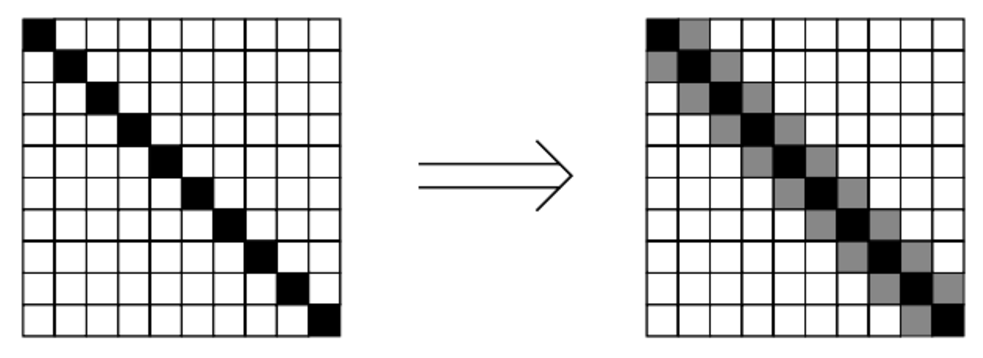
\includegraphics[scale=0.6]{Figs/Algorithms/diag}
\end{figure}

Предположим, например, что все $n$ клеток на главной диагонали инфицированы.
Тогда инфекция распространится на соседние диагонали и в итоге на всю доску.

Докажите, что нельзя заразить всю шахматную доску, если изначальное число инфицированных клеток меньше $n$.

\subsection*{Пустое ведро}% (EMPTYING A BUCKET)
\rindex{Пустое ведро}

Имеются три больших ведра, в каждом налито целое число унций жидкости.
В любой момент вы можете удвоить объём жидкости в одном из вёдер, долив туда из ведра с б\'{о}льшим объёмом жидкости.
Другими словами, разрешается переливать из ведра, содержащего $x$ унций жидкости, в ведро, содержащее 
$y\le x$ унций, до тех пор, пока там не станет $2y$ унций (а в первом ведре останется $x-y$).

\begin{figure}[h!]
\centering
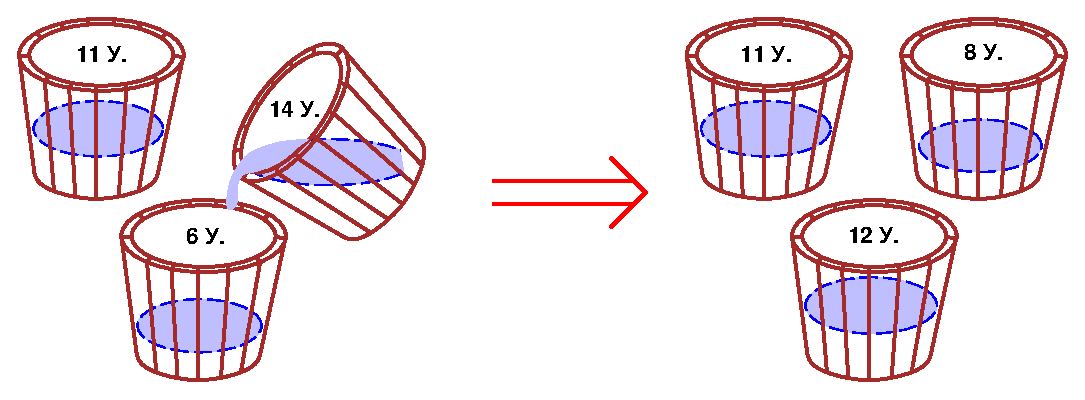
\includegraphics[scale=0.6]{Figs/Algorithms/buckets-ru}
\end{figure}

Докажите, что, независимо от начального состояния, вы сможете вылить всю жидкость из одного из вёдер.

\subsection*{Фишки по углам}% (PEGS ON THE CORNERS)
\rindex{Фишки по углам}

Четыре фишки начинают ходить с углов некоего квадрата на плоскости.
В любой момент одна фишка может перепрыгнуть через другую,
встав на том же расстоянии с противоположной стороны.
Фишка, через которую перепрыгнули, остаётся на месте.
Возможно ли передвинуть все фишки так, чтобы они оказались в углах б\'{о}льшего квадрата?

\subsection*{Фишки на полуплоскости}% (PEGS ON THE HALF-PLANE)
\rindex{Фишки на полуплоскости}

На оси $X$ и ниже неё в каждой вершине целочисленной решётки координатной плоскости  стоит по фишке.
В любой момент фишка может перепрыгнуть через соседнюю с ней фишку (по горизонтали, вертикали или диагонали) и встать на следующую вершину решётки, при условии, что она не занята.
При этом фишка, через которую перепрыгнули, снимается с поля.

\begin{figure}[h!]
\centering
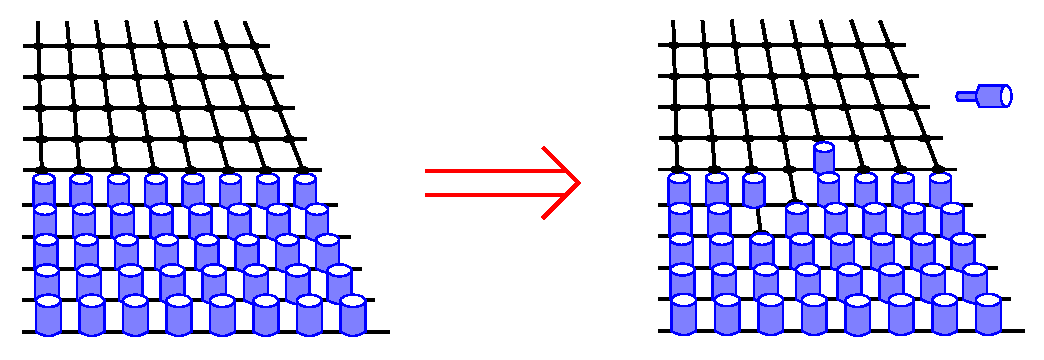
\includegraphics[scale=0.6]{Figs/Algorithms/pegs}
\end{figure}

Может ли фишка продвинуться произвольно далеко наверх от оси~$X$?

\subsection*{Фишки на квадрате}% (PEGS IN A SQUARE)
\rindex{Фишки на квадрате}

И снова фишки расположены в вершинах решётки на плоскости, только в этот раз в квадрате $n\times n$.
В данной задаче фишки могут прыгать только по горизонтали или вертикали, и фишка, через которую перепрыгнули, убирается с поля.
Цель задачи --- уменьшить число фишек с $n^2$ до $1$.

Докажите, что в случае, когда $n$ кратно $3$, этого сделать нельзя!

\subsection*{Кульбиты многоугольника}% (FLIPPING THE POLYGON)
\rindex{Кульбиты многоугольника}

Вершины многоугольника обозначены числами, сумма которых положительна.
В любой момент разрешается поменять знак у вершины с отрицательным числом, но тогда новое значение вычитается из обеих чисел, обозначающих соседние вершины, так чтобы сумма оставалась постоянной.

\begin{figure}[h!]
\centering
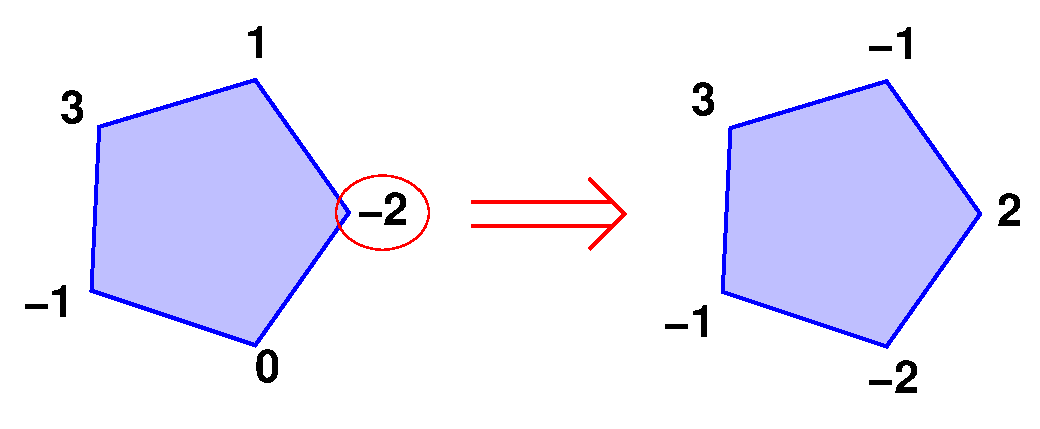
\includegraphics[scale=0.6]{Figs/Algorithms/pent}
\end{figure}

Докажите, что вне зависимости от порядка выбора чисел, после конечного числа шагов все числа окажутся положительными, и, таким образом, процесс прекратится.

\subsection*{Лампочки по кругу}% (LIGHT BULBS IN A CIRCLE)
\rindex{Лампочки по кругу}

Лампочки расставлены по кругу и пронумерованы от $1$ до $n$.
Изначально они все включены.
В момент времени $t$ вы смотрите на лампочку номер $t \pmod{n}$, и, если она включена, то меняете состояние у лампочки $t + 1 \pmod{n}$;
то есть выключаете её, если она включена, и включаете, если она выключена.
Если лампочка $t$ выключена, то вы ничего не делаете.

Докажите, что если ходить и ходить по кругу подобным образом, то в конце концов наступит момент, когда все лампочки снова будут включены.

\subsection*{Жуки на многограннике}% (BUGS ON A POLYHEDRON)
\rindex{Жуки на многограннике}

На каждой грани выпуклого многогранника живёт по жуку.
Жуки ползают по периметру своей грани с разными скоростями, но только по часовой стрелке.
Докажите, что невозможно создать такое расписание, чтобы жуки могли обойти свою грань и вернуться к начальной точке, ни с кем не столкнувшись.

\subsection*{Жуки на числовом луче}% (BUGS ON THE LINE)
\rindex{Жуки на числовом луче}

В каждой положительной целочисленной точке на числовом луче стоит зелёная, жёлтая или красная лампочка.
Жук ставится на начало луча и ползёт, подчиняясь следующим правилам:
\begin{itemize}
\item если он видит зелёный свет, он переключает его на жёлтый и передвигается на один шаг вправо; 
\item если он видит жёлтый свет, он переключает его на красный и передвигается на один шаг вправо; 
\item если же он видит красный свет, он переключает его на зелёный и передвигается на один шаг \emph{влево}.
\end{itemize}

В конце концов, жук либо свалится с левого конца, либо уползёт на бесконечность вправо.
Затем второй жук ставится на начало луча, затем третий.

Докажите, что если второй жук свалился с левого конца, то третий жук уползёт на бесконечность.

\subsection*{Как разломать шоколадку}% (BREAKING A CHOCOLATE BAR)
\rindex{Как разломать шоколадку}

Дана шоколадка из $m\times n$ квадратных долек. 
Требуется разломать её на составные дольки.
За один шаг вы можете взять один кусок и разломить его по вертикальной или горизонтальной линии.

Докажите, что какой бы вы метод ни выбрали, вам потребуется одно и то же  число шагов.

\begin{figure}[h!]
\centering
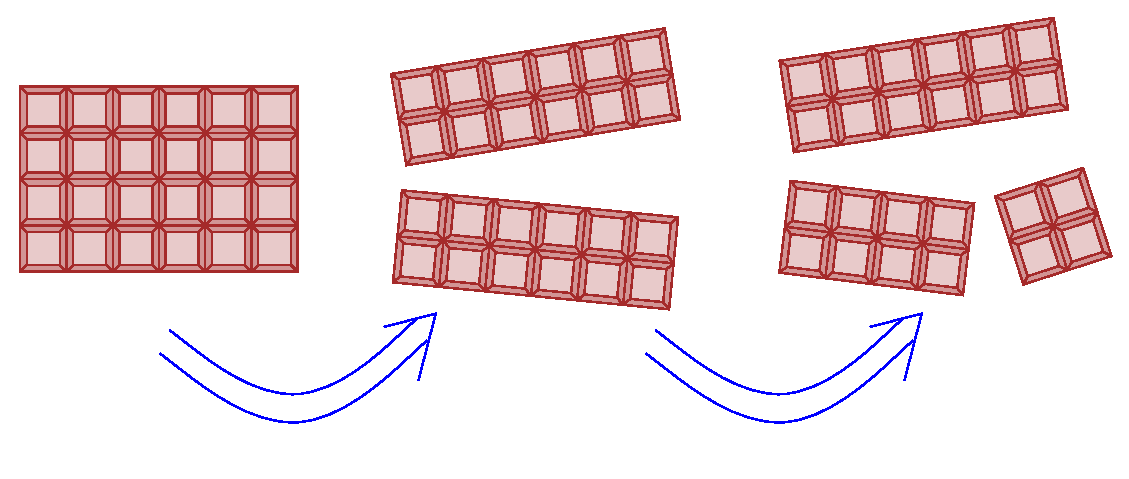
\includegraphics[scale=0.5]{Figs/Algorithms/bar}
\end{figure}

\section*{Решения и комментарии}

\subsubsection*{Инфекция на шахматной доске}% (THE INFECTED CHECKBOARD)

{\sloppy

Эта милая задача появилась на Московской городской олимпиаде в 1986 году,%
\footnote{Задачи XLIX Московской городской математической олимпиады, \emph{Квант} 1986, № 8, с. 57.}
а затем перекочевала в Венгрию.\footnote{Gábor Pete: Hogyan gyepesítsünk kockát? \emph{Polygon (Szeged)} VII:1 (1997), 69--80.}
В случае произвольного расположения начальных клеток такой процесс называется \emph{двухмерной бутстрепной перколяцией}.
Прекрасный математический анализ этого процесса был сделан Анде Холройдом (ныне профессор Университета Британской Колумбии).%
\footnote{A. Holroyd, ``Sharp metastability threshold for two-dimensional bootstrap percolation''. \emph{Probab. Theory Related Fields} 125 (2003), no. 2, 195--224.}
Эта задача попала ко мне от Джоэла Спенсера %Joel Spenser, NYU) 
из Нью-Й\'{о}ркского университета, который утверждал, что существует «решение в одну строку»!
Как вы увидите, это не слишком большое преувеличение.

}

{

\begin{wrapfigure}{r}{36mm}
\vskip-8mm
\centering

\includegraphics[scale=1.5]{Figs/Algorithms/sick}
\end{wrapfigure}

\medskip

Пример с диагональю может натолкнуть на неверный путь, когда пытаются доказать, что в начальный момент инфицированные клетки должны быть в каждой строке или столбце.
Но это далеко не так.
Например, при расположении инфицированных клеток, как показано на рисунке, заражается вся доска.

}

Существует великое множество способов заразить всю доску при помощи $n$ изначально инфицированных клеток, но, оказывается, нету способа сделать это с меньшим числом.
Здесь нужен магический параметр $P$, но какой?

Этот параметр --- периметр!
Когда клетка заражена, по меньшей мере, две из её сторон сливаются с внутренностью заражённой территории, и максимум две стороны добавляются к её границе.
Следовательно, периметр заражённой территории не может увеличиваться.
Поскольку периметр всей доски равен $4n$ (предполагая, что клетки единичные), начальная заражённая территория должна содержать минимум $n$ клеток.
\heart

Дополнительное упражнение для тех, кому интересно: докажите, что $n$ изначально инфицированных клеток необходимо даже тогда, когда верх и низ доски склеены так, что получился цилиндр.
Если же ещё склеить правую и левую стороны так, что получится тор, то достаточно (и необходимо) $n-1$ изначально инфицированных клеток.
Периметр здесь больше не поможет,
работает другой подход, найденный Брюсом Рихтером (университет Ватерлоо) %(Bruce Richter, University of Waterloo) 
и вашим автором.

\subsubsection*{Пустое ведро}% (EMPTYING A BUCKET)

Ещё одна красивая задача из бывшего Советского Союза, которая была представлена на V-й Всесоюзной математической олимпиаде в Риге в 1971 году.
Позже она появлялась (уже без хозяйственного инвентаря), на Математической олимпиаде Патнема 1983 года.
Задача попала ко мне от Кристиана Боргса из лабораторий «Microsoft Research». %(Christian Borgs of Microsoft Research).
Я покажу два решения --- одно моё, комбинаторное, и второе, элегантное, теоретико-числовое доказательство, найденное Сванте Янсоном из Уппсальского университета, Швеция %(Svante Janson of Uppsala University, Sweden)
(а также независимо от него, Гартом Пэйном). %(Garth Payne)).
Я не знаю, которое из двух решений, если не третье, предполагалось изначально.

\medskip

В решении Сванте, за параметр $P$ берётся содержимое конкретного ведра и показывается, как можно каждый раз уменьшать $P$ и довести его до нуля.
В моём доказательстве, напротив, показывается, как можно каждый раз \emph{увеличивать} $P$ до тех пор, пока одно из \emph{оставшихся} вёдер не окажется пустым.

Чтобы доказать последнее утверждение, во-первых, отметим, что можно предположить, что только одно из вёдер содержит нечётное число унций жидкости.
Действительно, если нету «нечётных» вёдер, то можно изменить шкалу, разделив объёмы на степень двойки.
Если же имеется больше двух «нечётных» вёдер, то первый же шаг с двумя из них сократит их число до одного или нуля.

Во-вторых, заметим, что с нечётным и чётным ведром всегда можно сделать \emph{обратный ход}, то есть вылить половину содержимого чётного ведра в нечётное.
Действительно, каждое состояние этой пары вёдер может быть достигнуто максимум из одного состояния, таким образом, после достаточного числа шагов вы пройдёте по циклу и вернётесь в начальное состояние.
Состояние \emph{прямо перед} тем, как вы возвращаетесь к начальному, и является результатом вашего «обратного хода».

И последнее, мы утверждаем, что, пока нет пустого ведра, содержимое нечётного ведра всегда можно увеличить.
Если есть ведро, у которого число унций содержимого делится на 4, то обратным ходом можно половину его перелить в нечётное ведро.
Если же такового нет, то его легко получить, совершив одну операцию между двумя чётными вёдрами.
\heart

А вот доказательство Сванте, в его собственном изложении:

\medskip

«Обозначим число унций жидкости, которое изначально содержалось в вёдрах $A$, $B$ и $C$ через $a$, $b$ и $c$, где $0<a\le b\le c$.
Я опишу последовательность шагов, приводящую к тому, что минимальный из трёх объёмов жидкости станет меньше, чем $a$.
Если минимум равен нулю, то задача решена; в противном случае, мы переобозначаем вёдра и повторяем процедуру.

Пусть $b = qa + r$, где $0\le r<a$ и $q\ge 1$ --- целое число.
Запишем $q$ в двоичной системе: $q=q_0+2q_1+\dots+2^nq_n$, где каждое $q_i$ это $0$ или $1$, и $q_n = 1$.

Проделаем $n+1$ шаг, пронумеровав их $0,\dots, n$ следующим образом: на $i$-м шаге  мы выливаем из $B$ в $A,$ если $q_i = 1$, и из $C$ в $A$, если $q_i = 0$.
Поскольку мы всё время льём в $A$, его содержимое каждый раз удваивается, так что $A$ содержит $2^ia$ перед $i$-м шагом.
Отсюда общий объём жидкости, вылитый из $B$ равен $qa$, таким образом, в конце $b-qa=r<a$ остаётся в $B$.
Заметим, что общий объём жидкости, вылитый из $C$ равен, максимум
\[\sum_{i=0}^{n-1} 2^ia<2^na\le qa\le b\le c.\]
Таким образом, в $C$ (и в $B$) достаточно жидкости, чтобы проделать все эти шаги.»
\heart

Насколько мне известно, никто не знает даже приблизительно, сколько требуется шагов для решения этой задачи (в худшем начальном состоянии с общим объёмом жидкости равным $n$ унциям).
Моё решение показывает, что достаточно порядка $n^2$ шагов.
Свантевское  решение лучше, оно ограничивает число шагов произведением константы на $n\log n$.
Окончательный ответ может оказаться ещё меньше.

\subsubsection*{Фишки по углам}% (PEGS ON THE CORNERS)

На эту симпатичную задачу обратил моё внимание Миккель Торуп из лабораторий AT\&T, %(Mikkel Thorup of AT&T Labs),
который её услышал от Ассафа Наора %(Assaf Naor)
(в то время научного сотрудника Майкрософта), который услышал её от аспирантов Еврейского университета в Иерусалиме.

\medskip

Заметим, что если фишки начинают ходить с вершин решётки (то есть точек плоскости с целыми координатами), то они всегда будут оставаться в вершинах решётки.

В частности, если изначально они располагаются в вершинах единичного квадрата решётки, то они, разумеется, не могут позже оказаться в углах \emph{меньшего} квадрата, поскольку в решётке не существует квадратов, меньше единичного.
Но почему не в углах б\'{о}льшего квадрата?

Основное наблюдение: прыжок через фишку обратим!
Если бы было возможно прийти к б\'{о}льшему квадрату, то мы могли бы обратить весь процесс и завершить ход на меньшем квадрате, что, как мы уже знаем, невозможно.
\heart

\subsubsection*{Фишки на полуплоскости}% (PEGS ON THE HALF-PLANE)

Это вариант задачи, описанной во втором томе «Выигрышных стратегий ваших математических игр».\footnote{E. Berlekamp, J. Conway, R. Guy,
\emph{Winning Ways for your Mathematical Plays.} Academic Press, 1982.}
Мы полагаем, задача была изначально придумана одним из авторов книги, Джоном Конвеем.
В его варианте не разрешались прыжки по диагонали, тем не менее, можно было без особых трудностей продвинуть фишку до линии $y = 4$.
Рассуждение, подобное приведённому ниже, показывает, что позиции выше достичь невозможно.

\medskip

С прыжками по диагонали или без, трудность состоит в том, что когда фишки поднимаются выше, вершины решётки под ними оголяются.
Нам нужен такой параметр $P$, который бы получал награду за ушедшую высоко фишку, но для компенсации подвергался бы наказанию за оставленные позади дырки.
Естественным выбором была бы сумма по всем фишкам некоторой функции от их позиции.
Поскольку фишек бесконечно много, необходимо позаботиться, чтобы сумма сходилась.

Например, фишке на $(0, y)$ можно присвоить вес $r^y$, где $r$ --- некое вещественное число большее $1$.
Так, что веса фишек на нижней части оси $Y$ в сумме дадут конечное число $\sum_{y\le 0}r^y = r/(r-1)$.
Веса в прилегающих столбцах нужно будет уменьшать, чтобы сумма по всей плоскости оставалась конечной.
Если на каждом шаге при удалении от оси $Y$ мы делим вес на $r$, то получаем, что вес фишки в точке $(x, y)$ равен $r^{y - |x|}$, и тогда общий вес в начальной позиции 
\[\frac r{r-1} + \frac 1{r-1} +\frac 1{r-1} +\frac 1{r(r-1)} +\frac 1{r(r-1)} + \dots =\frac{r^2+r}{(r-1)^2} <\infty.\]

Если фишка прыгнула, то в лучшем случае (когда прыжок был совершён по диагонали вверх к оси $Y$), $P$ приобретает $vr^4$ и теряет $v+vr^2$, где $v$ --- вес фишки перед прыжком.
Пока $r$ не превышает квадратный корень \emph{золотого сечения} $\varphi=(1+\sqrt5)/2\approx 1{,}618$, удовлетворяющего уравнению $\varphi^2=\varphi+1$, этот прирост не может быть положительным.

Далее, если положить $r = \sqrt{\varphi}$, то начальное значение $P$ составит примерно $39{,}0576$, но вес одной фишки в точке $(0, 16)$ \emph{сам по себе} равен $\varphi^8\approx 46{,}9788$.
Поскольку мы не можем увеличить $P$, то, следовательно, мы не можем продвинуть фишку на точку $(0, 16)$.

Но если бы мы смогли продвинуть фишку на \emph{любую} точку линии $y = 16$ или выше, то мы бы смогли попасть и в точку $(0, 16)$, остановив фишку, дошедшую до точки $(x, 16)$, и, повторив те же шаги на поле, сдвинутом вправо или влево на~$|x|$.
\heart

{\sloppy 

Нам неизвестно наибольшее значение $y$-координаты точки, до которой может дойти фишка при разрешённых диагональных прыжках.
Вполне возможно, какой-нибудь трудолюбивый читатель сможет устранить этот пробел.

}

\subsubsection*{Фишки на квадрате}% (PEGS IN A SQUARE)

Существует несколько способов решения данной задачи, которая является \emph{частью} задачи, представленной на Международной Математической Олимпиаде 1993 года.
Приведённое ниже доказательство мне рассказал Бенни Судаков из Принстонского университета.

\medskip

Покрасим вершины $(x, y)$ решётки в серый цвет, если ни $x$, ни $y$ не делятся на $3$, в противном случае --- в белый цвет.
Получается периодический узор из серых квадратов $2\times 2$ (см. рисунок). 

Если две соседние (ортогонально) фишки стоят обе в серых вершинах решётки или обе в белых, то фишка, оставшаяся после прыжка, окажется в белой вершине.
Если же одна вершина серая, а другая белая, то, напротив, фишка, оставшаяся после прыжка, будет стоять в серой вершине.
Из этого следует, что если изначально в серых вершинах находится чётное число фишек, то это свойство будет сохраняться.

\begin{figure}[h!]
\centering
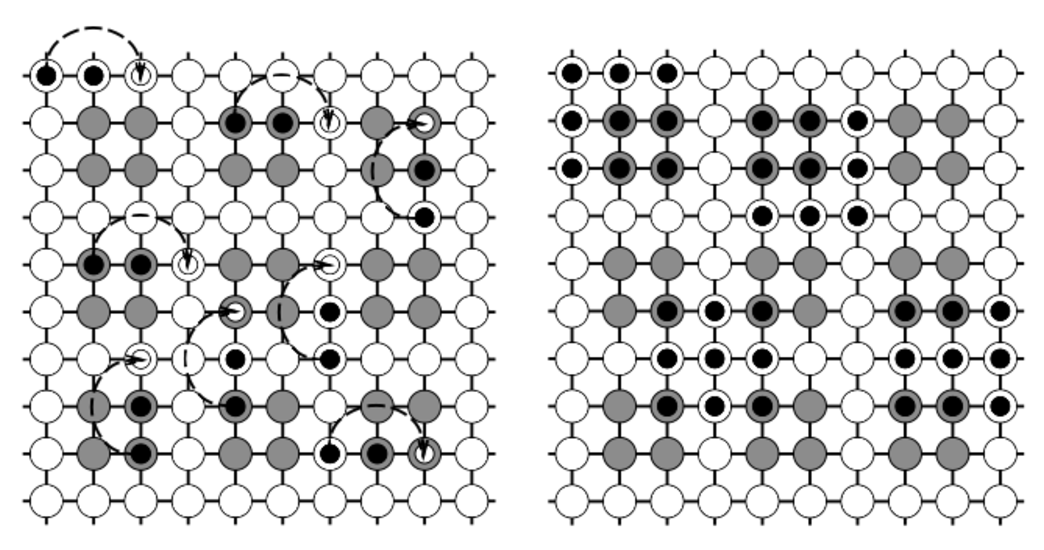
\includegraphics[scale=0.5]{Figs/Algorithms/square}
\end{figure}

Несложно увидеть, что если взять квадрат с фишками $3\times 3$ и поместить его на плоскость, то в какое бы место решётки мы его не определили, он всегда накроет чётное число серых вершин.
А так как квадрат $n\times n$, где $n$ кратно $3$, состоит из подобных квадратов, то в нём также всегда будет содержаться чётное число серых вершин.
Предположим, что оказалось возможным уменьшить число фишек в таком квадрате до одной.
Тогда мы смогли бы передвинуть начальный квадрат так, чтобы выжившая фишка оказалась в серой вершине. 
Это противоречие завершает доказательство.
\heart

Есть довольно техническое, не особенно простое и некрасивое, 
доказательство того, что если $n$ \emph{не} делится на $3$, то \emph{возможно} уменьшить число фишек до одной.
На олимпиаде участников просили точно определить, при каких $n$ квадраты можно свести к одной фишке --- довольно сурово требовать сделать это вот так сразу!

\subsubsection*{Кульбиты многоугольника}% (FLIPPING THE POLYGON)

Данная головоломка является обобщением задачи, появлявшейся на Международной Математической Олимпиаде 1986 года (представленной, как мне говорили, составителем из восточной Германии) и впоследствии получившей название «Задача о пентагоне».

Задача имеет много решений.
Более того, её можно обобщить и дальше, от $n$-угольников до произвольных связных графов.
Однако, решение, приводимое ниже, выделяется среди прочих сочетанием элегантности и строгости доказательства.
Его придумали, независимо друг от друга, хотя бы два математика, один из них --- Бернар Шазель, профессор информатики Принстонского университета. %(Bernard Chazelle, Professor of Computer Science at Princeton University)

\medskip

Пусть $x(0),\dots,x(n-1)$ --- числа при вершинах, дающие в сумме $s > 0$, с индексами, взятыми по модулю $n$.
Определим двустороннюю бесконечную последовательность
$b(\cdot)$, где $b(0) = 0$ и $b(i) = b(i -1) + x(i \mod{n})$.
Последовательность $b(\cdot)$ не является периодической, но она периодически возрастает: $b(i + n) = b(i) + s$.

\begin{figure}
\centering
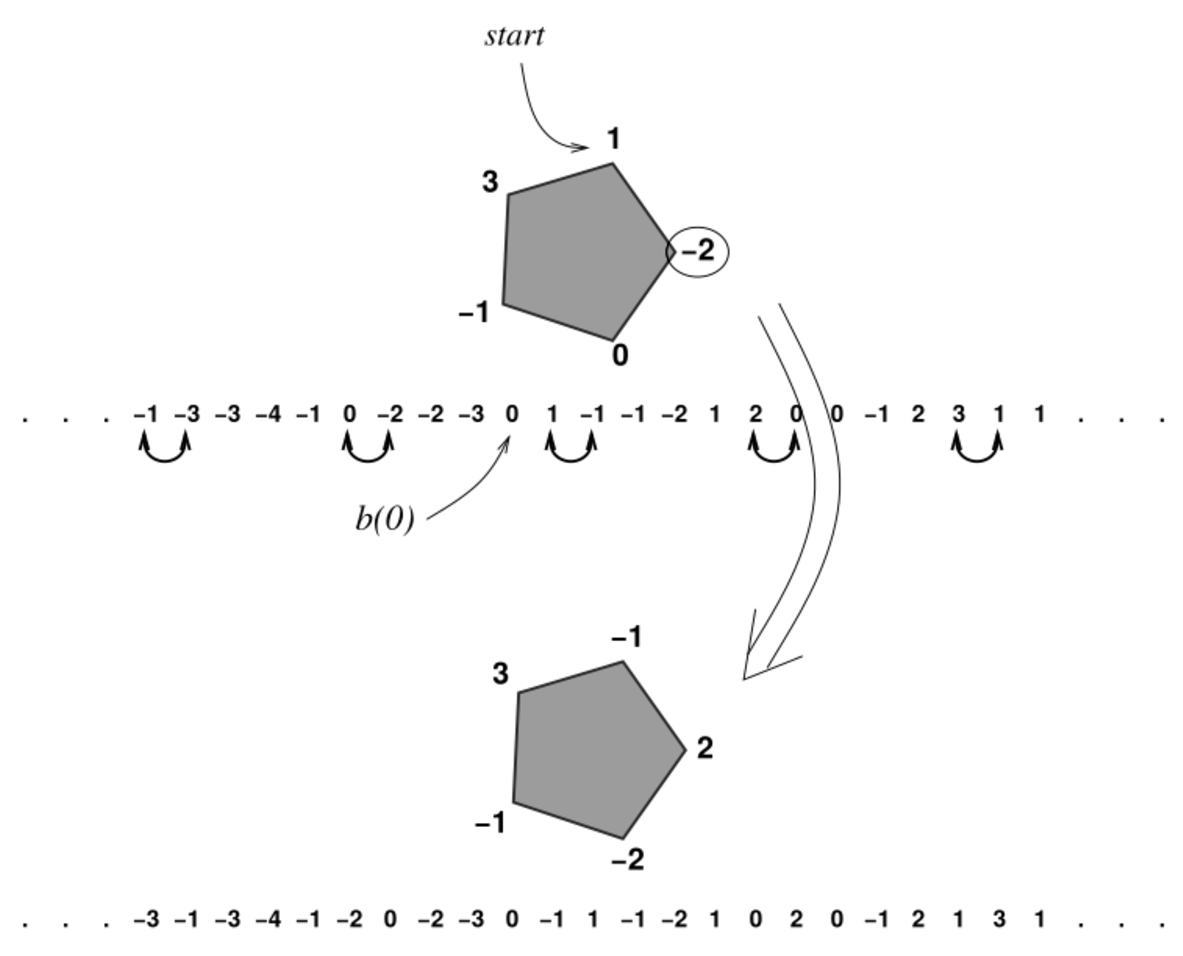
\includegraphics[scale=0.5]{Figs/Algorithms/sort}
\end{figure}

Если $x(i)$ --- отрицательно, то $b(i) < b(i-1)$, и, меняя знак у $x(i)$, получаем тот же эффект, как при замене $b(i)$ на $b(i - 1)$, так что они располагаются теперь в возрастающем порядке.
Это верно и для всех пар $b(j)$, $b(j - 1)$, сдвинутых на числа, кратные $n$.
Таким образом, изменение знака при вершине сводится к упорядочиванию $b(\cdot)$, используя перестановки соседних членов!

Чтобы проследить за ходом процесса сортировки, нам нужен некий конечный параметр $P$, который измеряет степень, при которой $b(\cdot)$ нарушает порядок. % (out of order).
Для нахождения его, положим $i^+$ --- число индексов $j > i$, для которых $b(j) < b(i)$, и $i^-$ --- число индексов $j < i$, для которых $b(j) > b(i)$.
Обратите внимание, что $i^+$ и $i^-$ имеют конечное значение и зависят только от $i \pmod n$.
Также отметим, что 
\[\sum_{i=0}^{n-1}i^+=\sum_{i=0}^{n-1}i^-\]
и пусть эта сумма будет нашим волшебным параметром $P$.

Когда $x(i+1)$ меняет знак, $i^+$ уменьшается на $1$, а все другие $j^+$ не меняются.
Значит, $P$ уменьшается \emph{в точности} на 1.
Когда $P$ достигает $0$, последовательность полностью отсортирована, так что все числа у вершин неотрицательны, и процесс прекращается.

Мы доказали больше, чем требовалось:
независимо от выбора чисел в этом процессе, он заканчивается за одно и тоже ($P$) число шагов,
более того, конечная конфигурация также не зависит от порядка выбора чисел!
Причина этого кроется в том, что существует только один способ сортировки $b(\cdot)$.
Когда сортировка завершена, член исходной последовательности $b(i)$ должен оказаться в позиции $i \z+ i^+ - i^-$.
\heart

\subsubsection*{Лампочки по кругу}% (LIGHT BULBS IN A CIRCLE)

Эта головоломка является частью задачи, представленной на Международной Математической Олимпиаде 1993 года.
При неуказанном значении $n$ лучшим способом решения будет показать (как мы это уже делали в одном из доказательств «Пустого ведра»), что само пространство состояний является циклическим.

\medskip

Во-первых, отметим, что нет опасности выключить все лампочки,
ведь если это изменение сделано в момент времени $t$, то лампочка номер $t$ всё ещё включена.

Более того, если мы посмотрим на наш круг сразу \emph{после} момента $t$, то узнаем, в каком состоянии были лампочки в момент~$t$ (изменив состояние лампочки $t+1$, если лампочка $t$ включена).
Поскольку число возможных состояний в круге конечно (мы учитываем, какая лампочка рассматривается, а также какие лампочки включены), то мы со временем должны будем повторить некое состояние в первый раз.
Скажем, в момент времени $t_1$ повторилось состояние, бывшее в момент $t_0$, где $t_1$ и $t_0$ отличаются на число, кратное $n$.
Но тогда в момент $t_1 - 1$ мы уже были в том же состоянии, как и в момент $t_0 - 1$, что является противоречием, если только момента $t_0 - 1$ не существовало.
А это значит, что $t_0=0$, то есть повторилось состояние, когда все лампочки были включены.
\heart

\subsubsection*{Жуки на многограннике}% (BUGS ON A POLYHEDRON)

Данная задача была представлена в статье Антона Клячко.%
\footnote{A. Klyachko, ``А Funny Property of Sphere and Equations over Groups''. \emph{Communications in Algebra}, Vol. 21, No. 7 (1993), 2555--2575.} 
Для её решения мы, по сути, должны сделать противоположное тому, что делали в предыдущей задаче, то есть показать, что некий параметр будет всегда меняться в одном направлении, и, таким образом, мы не сможем вернуться в исходное состояние.

\medskip

Заметим, что можно предположить, что в начальный момент ни один жук не стоит в вершине (можно жуков слегка подтолкнуть или придержать).
Можно также предположить, что, никакая пара жуков не проходит через вершины одновременно.

\begin{figure}[h!]
\centering
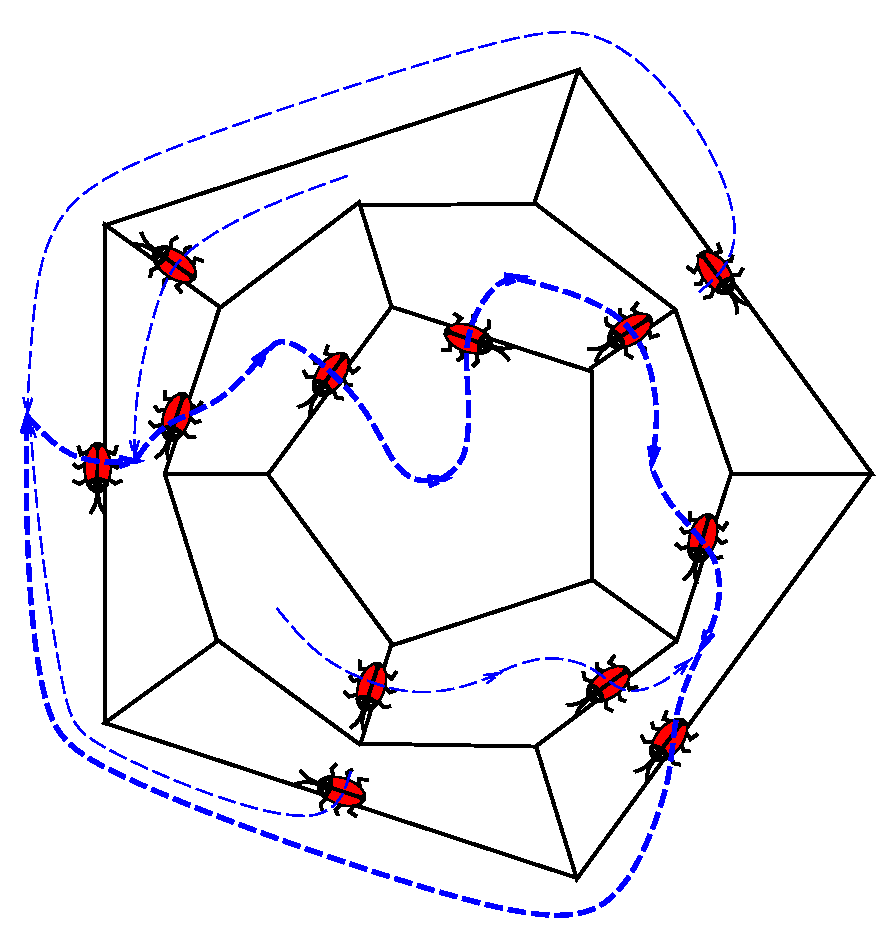
\includegraphics[scale=0.5]{Figs/Algorithms/dodec}
\end{figure}

В любой момент времени можно нарисовать стрелку из центра каждой грани $F$ к жуку с этой грани и дальше, к центру грани с другой стороны от жука.
Начав с любой грани и следуя далее по таким стрелкам, мы должны будем, в конце концов, оказаться на некой грани второй раз, завершив цикл стрелок на многограннике.

Этот цикл разделяет поверхность многогранника на две части.
Назовём внутренней частью цикла ту, которую мы обходим по часовой стрелке.
Обозначим через $P$ число вершин многогранника внутри цикла.

Изначально $P$ могло принимать любое значение от $0$ до числа всех (скажем, $n$) вершин многогранника.
Экстремальные значения получаются, когда два жука ползут по одному ребру, и, следовательно, длина цикла равна $2$.
В случае, когда $P=0$, два жука ползут по ребру навстречу друг другу, и столкновение неизбежно.

В момент, когда один из жуков в цикле переходит на следующее ребро, стрелка, проходящая через него, поворачивается вправо.
Вершина, через которую он переползает, бывшая до того внутри цикла, оказывается теперь снаружи.
Другие вершины также могли перейти из внутренней части цикла во внешнюю, но не существует способа перейти из внешней части во \emph{внутреннюю}.
Чтобы это увидеть, заметьте, что новая стрелка теперь направлена внутрь цикла.
У последовательности стрелок, исходящих из её конца, нет никакой возможности избежать зацикливания, они неизбежно придут к началу какой-то стрелки цикла, создав новый цикл с меньшей внутренней частью.
В частности, значение $P$ уменьшилось хотя бы на~$1$.

{

\sloppy

Поскольку $P$ не сможет принять своё начальное значение, нам остаётся только надеяться, что у жуков имеется страховка от несчастного случая.
\heart

}

\subsubsection*{Жуки на числовом луче}% (BUGS ON THE LINE)

Для начала нам нужно убедиться, что жук \emph{либо} свалится с левого конца луча, либо убежит на бесконечность вправо, то есть он не может вечно ползать туда-сюда.
Для этого ему пришлось бы проходить через какие-то числа бесконечное число раз.
Пусть $n$ --- наименьшее из таких чисел.
Здесь необходимо отметить, что попадая каждый третий раз на число $n$, жук увидит там красный свет, и следовательно, будет вынужден уползти влево на $n-1$, а это противоречит предположению, что он посетил $n-1$ только конечное число раз.

Теперь, когда с этим всё ясно, будет полезным думать о зелёном свете, как о цифре 0, о красном, как о 1, и о жёлтом, как это ни парадоксально, как о «цифре» $\tfrac12$.
А расположение цветов лампочек может быть представлено как число между $0$ и $1$, записанное в двоичной системе
\[x = 0{,}\,x_1\,x_2\,x_3\dots;\]
то есть,
 \[x = x_1\cdot(\tfrac12)+x_2\cdot(\tfrac12)^2+\dots\]
Будем думать о жуке в точке $i$, как о дополнительной «1» к $i$-й позиции, определяемой как
\[y=x+(\tfrac12)^i.\]
Ключевое наблюдение состоит в том, что $y$ является \emph{инвариантом}, то есть его значение не меняется при передвижении жука.
Если жук идёт вправо от точки $i$, то значение числа, на котором он сидел, поднимается на $\tfrac12$.
Следовательно, $x$ увеличивается на $(\tfrac12)^{i+1}$, а собственное значение жука уменьшается на ту же самую величину.
Если жук идёт налево от $i$, он увеличивает своё значение на $(\tfrac12)^i$ и это компенсируется тем, что значение $x$ уменьшается на целую цифру в $i$-й позиции.

Исключение составляет только момент, когда жук сваливается с левого конца луча.
В этом случае и $x$, и собственное значение жука уменьшаются на $\tfrac12$, то есть общая потеря равна $1$.
Когда выставляется следующий жук, $y$ увеличивается на $\tfrac12$.
Другими словами, значение $x$ поднимается на $\tfrac12$, если выставляется новый жук, и он исчезает справа на бесконечности; и $x$ падает на $\tfrac12$, если выставляется новый жук, и он сваливается с левого конца луча.

Конечно же, в любой момент $x$ должен лежать в единичном интервале.
Если его начальное значение лежит строго между $0$ и $\tfrac12$, то жуки должны будут поочерёдно убегать направо, падать слева, убегать, падать и так далее.
Если же $x$ лежит строго между $\tfrac12$ и $1$, то жуки поочерёдно будут падать, убегать, падать, убегать и так далее.

Оставшиеся случаи можно проверить руками.
Если изначально $x = 1$ (все точки --- красные), первый жук переключит $1$ на зелёный и свалится слева.
Второй жук, вихляя, удаляется вправо на бесконечность, оставив все лампочки опять красными, то есть мы получим чередование: падает, убегает, падает, убегает...

Если $x = 0$ (то есть все точки --- зелёные), то первый жук убежит, второй опять убежит (так как все точки сменятся на жёлтые, а потом на все красные), а затем чередование --- падает, убегает, падает, убегает..., как и прежде.

Самый интересный случай --- это $x=\tfrac12$, так как существует несколько способов представления $\tfrac12$ в нашей модифицированной двоичной системе: $x$ может быть составлен из одних $\tfrac12$, или он может начинаться с любого конечного числа (включая ноль) $\tfrac12$, за которым следуют либо $0111\dots$, либо $1000\dots$.
В первом случае начинающий жук переключит все жёлтые лампочки на красные по мере удаления направо, таким образом, мы получаем чередование  убегает, падает, убегает, падает...
Второй случай такой же, первый жук, вихляя, уползает направо, опять оставляя все точки после себя красными.
В третьем случае жук переключает жёлтый на красный по ходу движения, но когда он достигает красной точки, он разворачивается и двигается налево, меняя красный на зелёный по пути, пока не свалится с конца луча.
После этого приходим к случаю $x = 0$, так что в этом случае  последовательность будет: падает, убегает, падает, убегает...

Возвращаясь опять ко всем случаям, мы видим, что всякий раз, когда второй жук падает, третий жук убегает.
\heart

Это элегантное рассуждение представили
Анде Холройд (Университет Британской Колумбии) и Джим Пропп (Висконсинский университет) на встрече группы «Институт Элементарных Исследований» в Баннфе, Альберта в 2003 году. %
%\footnote{прим. перев.: \href{https://www.birs.ca/files/scientific-reports/}{\url{www.birs.ca/files/scientific-reports/BIRS_SR_2003.pdf}} стр. 63}
Пропп предложил использовать жука, чтобы детерминизированно смоделировать случайные блуждания на неотрицательных целых числах, в которых шаги делаются (независимо) влево с вероятностью $\tfrac13$ и вправо с вероятностью $\tfrac23$.
В подобных блужданиях конкретный жук падает с левого конца луча или убегает на бесконечность вправо с одинаковой вероятностью.
Но как мы видели, детерминизированная модель показывает вместо этого, что после первой пары жуков направления строго чередуются.
Доказательство может быть обобщено и на другие виды случайных блужданий.

\subsubsection*{Как разломать шоколадку}% (BREAKING A CHOCOLATE BAR)

Эта до смешного простая задача известна тем, что некоторые \emph{очень} крутые математики зависали на ней на целый день, пока среди  стенаний и битья головой об стену на них не снисходило озарение.
Рискуя прослыть садистом, я пропускаю доказательство.

\chapter*{Ещё игры}
\addcontentsline{toc}{chapter}{Ещё игры}
%“Half this game is 90\% mental.”
%-- Danny Ozark manager of the Phillies baseball team.

\setlength{\epigraphwidth}{.6\textwidth}
\epigraph{Половина этой игры на 90\% идёт в уме.}{---Дэнни Озарк, тренер Филадельфийской бейсбольной команды.}

Вообще говоря, анализ игры часто требует решения двух задач: нахождения правильной стратегии и нахождения убедительного аргумента, который показывает, что стратегия наилучшая из возможных.
(Такой аргумент может быть правильной стратегией для другого игрока.)

Но, иногда можно отделаться довольно легко.
Рассмотрим следующую невинную с виду задачу.

\subsection*{Щёлк}% (CHOMP)
\rindex{Щёлк}

Два игрока по очереди откусывают от прямоугольной шоколадки, сотоящей из $m \times n$ квадратных долек.
Каждый раз игрок выбирает дольку и откусывает её вместе со всеми дольками находящимися сверху и справа от неё.
Каждый игрок старается избежать левую нижнюю дольку, которая отравлена.

Докажите, что если шоколадка состоит больше, чем из одной дольки, то у первого игрока есть выигрышная стратегия.

\begin{figure}[h!]
\centering
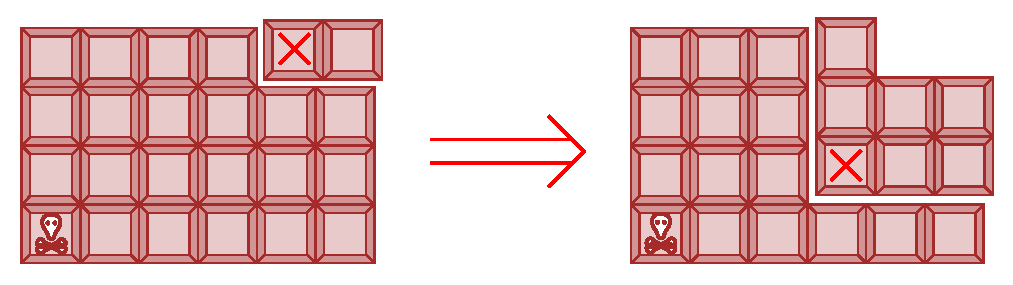
\includegraphics[scale=0.5]{Figs/MoreGames/chomp}
\end{figure}

\paragraph{Решение:} Либо у первого игрока (Алисы), либо у второго (Боба) должна быть выигрышная стратегия.
Предположим, она будет у Боба.
Тогда, в частности, у Боба должен быть выигрышный ответ на первый ход Алисы, когда она просто откусывает верхнюю дольку справа.

Но какой бы ни был ответ Боба, Алиса может сделать таким же свой первый ход, что противоречит предположению о том, что Боб всегда может выиграть.
Отсюда следует,
что выигрышная стратегия должна быть у Алисы.
\heart

Такой вид доказательства известен как \emph{заимствование стратегии} и он, к сожалению, ничего не говорит нам о том, как же, собственно, Алисе выигрывать игру.
В последней главе подробнее рассказывается об игре «Щёлк», её истории и более общей версии.

\medskip

Для решения оставшихся задач-игр используются разнообразные методы.

\subsection*{Детерминированный покер}% (DETERMENISTIC POKER)
\rindex{Детерминированный покер}

Не желая зависеть от капризного случая, Алиса и Боб решили сыграть в абсолютно детерминированную версию пятикарточного покера (так называемый дро-покер).
Колода карт раскладывается на столе в открытую.
Алиса выбирает 5 карт, затем Боб берёт 5 карт.
Алиса меняет любое число карт, заменённые карты выходят из игры, то же проделывает и Боб.
Все действия производятся в открытую на виду у оппонента.
Игрок с лучшей комбинацией выигрывает.
Поскольку Алиса ходит первая, то, если конечные комбинации оказываются равносильными, Боб объявляется победителем.
Кто победит при оптимальной игре?

\medskip

Детерминированный покер --- это игра с полной информацией.
В играх, содержащих скрытую информацию или одновременные ходы, может потребоваться вероятностная стратегия.
Говорят, что набор таких стратегий (один для каждого игрока) находится в \emph{равновесии}, если никто из игроков не может увеличить выигрыш, изменив свою стратегию, при условии, что остальные участники своих стратегий не меняют.
Например, в игре «Камень, ножницы, бумага» в (единственной) равновесной стратегии, каждый игрок выбирает все три возможных варианта с одинаковой вероятностью.

\subsection*{Шведская лотерея}% (SWEDISH LOTTERY)
\rindex{Шведская лотерея}

Для Шведской национальной лотереи предлагался следующий механизм игры: каждый участник выбирает целое положительное число.
Тот, кто называет наименьшее число, никем другим не выбранное, объявляется победителем.
(Если нет числа, выбранного только одним участником, то победителя нет.)

Если в игре участвуют только три человека, и каждый применяет оптимальную, равновесную, вероятностную стратегию, чему равно наибольшее положительное число, имеющее положительную вероятность быть выбранным?

\subsection*{Блины}% (PANCAKES)
\rindex{Блины}

Алиса и Боб опять проголодались, и перед ними лежат две стопки блинов, высотой в $m$ и $n$ блинов.
Каждый игрок по очереди должен съесть из большей стопки число блинов (ненулевое), кратное количеству блинов в меньшей стопке.
Разумеется, последний блин в каждой стопке непропечённый, так что игрок, который первым заканчивает стопку, проигрывает.

Для какой пары $(m,n)$ у Алисы (она ходит первая) имеется выигрышная стратегия?

Что случается, если у игры обратная цель, то есть побеждает тот, кто первый закончит стопку?

\subsection*{Определение разности}% (DETERMINING A DIFFERENCE)
\rindex{Определение разности}

После завтрака Алиса и Боб решают отдохнуть и сыграть в простую числовую игру.

\medskip

Алиса выбирает цифру и Боб подставляет её вместо звёздочки в выражение «$**** - ****$»; процедура повторяется пока остаются звёздочки. 
Алиса пытается сделать окончательную разность максимальной, a Боб --- минимальной.
Какая разность получится при оптимальной игре?

\subsection*{Тройная дуэль}% (THREE-WAY DUEL)
\rindex{Тройная дуэль}

Алиса, Боб и Кэрол устраивают тройную дуэль.
Алиса --- плохой стрелок, попадает в цель, в среднем, только в $\tfrac13$ случаев.
Боб лучше, попадает в цель с вероятностью $\tfrac23$.
Кэрол --- меткий стрелок, бьёт без промаха.

Они стреляют по очереди, первой Алиса, вторым Боб и третьей Кэрол, затем опять Алиса, и так далее, пока не останется только один стрелок.
Каков для Алисы наилучший план действий?

\section*{Решения и комментарии}

\subsubsection*{Детерминированный покер}% (DETERMENISTIC POKER)

{\sloppy

Немного о порядке комбинаций карт для данной задачи: и так, наилучшей комбинацией здесь является стрит-флэш (любые пять карт одной масти по порядку).
Стрит-флэш, начинающийся с туза (его также называют «Роял-флэш») бьёт стрит-флэш, возглавляемый королём, и так далее вниз по порядку.

}

Это означает, что если Бобу удастся собрать роял-флэш, то Алисина песенка спета.
Поэтому, чтобы получить шанс выиграть, Алисин первый набор карт должен содержать по одной карте каждого из четырёх возможных роял-флэшев.

Для этой цели лучшими картами являются десятки каждой масти, поскольку они не дают собрать стрит-флэш, начинающийся с десяти или с более высокой карты.
И действительно, поразмыслив минуточку, вы поймёте, что любая комбинация Алисы с изначальными четырьмя десятками выигрывает.
У Боба не остаётся надежды собрать стрит-флэш выше девятки.
Но чтобы не дать Алисе собрать роял-флэш, он должен взять, по меньшей мере, по одной карте выше десятки из каждой масти, и не более одной карты ниже десятки.
Алиса же теперь может поменять четыре карты и собрать стрит-флэш, начинающийся с десятки, в любой масти, кроме масти младшей карты Боба,
и Боб оказывается тут совершенно беспомощен.
\heart

У Алисы имеются также и другие выигрышные наборы комбинаций.
Эта странная игра обсуждалась в одной из ранних рубрик Мартина Гарднера. 

\subsubsection*{Шведская лотерея}% (SWEDISH LOTTERY)

Предположим, $k$ --- наибольшее число, которое готов выбрать каждый из игроков.
Если игрок выбирает $k$, он выигрывает, когда совпадает выбор двух других игроков, кроме случая, когда они также выбрали $k$.
Но если он выбирает $k+1$, то выигрывает каждый раз, когда выбор двух других совпадает, \emph{точка}.
Отсюда следует, что лучше выбрать $k+1$, чем $k$, и, значит, стратегия не равновесна.
Это противоречие указывает на то, что необходимо рассматривать произвольно большие числа --- иногда следует выбрать 1487564.
\heart

В равновесной стратегии каждый игрок должен выбрать число $j$ с вероятностью $(1-r)r^{j-1}$, где 
\[r = -\frac13-\frac2{\sqrt[3]{17+3\sqrt{33}}}+\frac{\sqrt[3]{17+3\sqrt{33}}}3,\]
что примерно равно $0{,}543689$.
Вероятности выбора 1, 2, 3 и 4 равны примерно $0{,}456311$, $0{,}248091$, $0{,}134884$ и $0{,}073335$, соответственно.

На эту довольно симпатичную идею лотереи обратил моё внимание Улле Хэггстрём из университета Чалмерса в Гётеборге, Швеция. %(Olle Häggström of Chalmers University in Göteborg, Sweden.)
Я не знаю, была ли эта идея осуществлена или хотя бы серьёзно рассматривалась в качестве официальной национальной лотереи; а вы не считаете, что стоило бы?

\subsubsection*{Блины}% (PANCAKES)

Положим, что в настоящий момент в стопках $m$ и $n$ блинов, и $m > n$.
Если соотношение размеров стопок $r = m/n$ лежит строго между 1 и 2, то на следующем ходу новое соотношение равно $\tfrac1{1-r}$.
Эти пропорции равны только если $r$ равно золотому сечению;
то есть $r=\phi=(1+\sqrt{5})/2\approx 1{,}618$.
Поскольку число $\phi$ иррационально, одно из двух соотношений $r$ и $\tfrac1{1-r}$ должно быть больше, а другое меньше~$\phi$.

Первый игрок (Алиса) выигрывает только тогда, когда начальное соотношение большей стопки к меньшей превышает $\phi$.
Чтобы это увидеть, предположим $m>\phi n$, но $m$ не кратно $n$.
Запишем $m=an+b$, где $0<b<n$.
Тогда: либо $n/b<\phi$, и в этом случае Алиса ест $an$ блинов, либо $n/b>\phi$, и в этом случае она съедает только $(a-1)n$ штук.
Боб остаётся с соотношением, меньшим $\phi$, и он вынужден сделать ход, который возвращает соотношению значение больше $\phi$.

Рано или поздно, Алиса достигнет момента, когда её соотношение $m/n$ --- целое число, и тогда она сможет уравнять число блинов в двух стопках и оставить Боба с сырым блином.
Заметим, что она также может, если захочет, забрать себе всю стопку блинов.

Разумеется, если вместо этого Алиса имеет дело с соотношением $m/n$, которое лежит строго между $1$ и $\phi$, она оказывается в безвыходном положении %( дело её --- швах)
и теперь Боб задаёт игру.

Приходим к заключению, что независимо от того, в какой вариант «Блинов» играют, если высоты стопок $m>n$, то Алиса выигрывает, в точности когда $m/n>\phi$.
Только в тривиальном случае, когда стопки изначально одинаковы, цель игры имеет значение.\heart

Данная задача была представлена на 12-й Всесоюзной математической олимпиаде в Ташкенте в 1978 году.
Мне её показал Билл Газарч из Мэрилендского университета.% (Bill Gasarch of the University of Maryland).

\subsubsection*{Определение разности}% (DETERMINING A DIFFERENCE)

Запишем эту разность как $x-y$, с $x=abcd$ и $y=efgh$.
В любой момент в игры, будем обозначать через $x(0)$ результат замены оставшихся звёздочек на нули, аналогично будем использовать обозначения $x(9)$, $y(0)$ и $y(9)$.

Алиса гарантированно может получить 4000, называя $4$-ки и $5$-ки, пока Боб не поставит цифру на позицию $a$, после чего Алиса выбирает нули до конца игры;
если же Боб ставит $4$-ку или $5$-ку на позицию $e$, то она заканчивает игру одними $9$-ками.
Ей нужно следить за тем, что $x(9)\ge y(9)$ всякий раз, когда она называет цифру 5, так как Боб может поставить $5$-ку на позицию $e$;
также она должна гарантировать, что $x(0)\ge y(0)$ каждый раз, когда выбирает цифру 4, иначе Боб поставит эту $4$-ку на позицию $a$.
Это можно проделать следующим образом.

Если в какой-то момент игры $x$ и $y$ одинаковы, то Алиса называет либо 4, либо 5.
В любой другой ситуации обозначим через $u$ и $v$, соответственно, самые левые отличные друг от друга позиции в $x$ и $y$.
Если $u=*$ (в этом случае $x(9)> y(9)$), то Алиса называет 5, если же $v=*$ (в этом случае $x(0)> y(0)$), то она называет 4.
Никогда не может случиться, что $u=4$ и $v=5$, а если $u=5$ и $v=4$, то выполняются оба неравенства $x(9)> y(9)$ и $x(0)> y(0)$, так что Алиса может смело выбирать либо 4, либо 5.

С другой стороны, Боб легко гарантирует себе 4000, если сразу же поставит 4 или меньшую цифру на позицию $a$, либо 5 или б\'{о}льшую цифру на позицию $e$.
Затем он не меняет первую звёздочку в другом числе, пока не появится не ноль (в первом случае) или не девять (во втором случае).
Таким образом он получит либо $4000-0000$, либо $9999-5999$, а, может, что-то получше.
\heart

Эта задача уходит своими корнями, по меньшей мере, к 6-й Всесоюзной математической олимпиаде в Челябинске 1972 года.

\subsubsection*{Тройная дуэль}% (THREE-WAY DUEL)

Об этой бородатой задаче мне напомнил Ричард Плотц из Провиденса, штат Род-Айленд.
%(Dr. Richard Plotz of Providence, RI)
У неё есть множество вариаций, одна из которых появилась в книге головоломок Хьюберта Филлипса 1938 года.\footnote{H. Phillips, \emph{Question Time},  J. M. Dent \& Sons, London, 1938}

\medskip

Совершенно очевидно, что Алиса не должна целиться в Боба --- если она попадёт, то на следующем шаге её подстрелит Кэрол --- конец игры.
В случае удачи с Кэрол, Алисе предстоит дуэль с Бобом, а Боб лучше попадает в цель, и стреляет он первым.
Шансы выжить у неё определённо меньше $\tfrac13$.

(На самом деле, если обозначить через $p$ вероятность остаться в живых у Алисы, в случае если Боб стреляет первым, а через $q$ --- вероятность (б\'{о}льшую) выживания Алисы, когда она стреляет первой, то $p=\tfrac13\cdot q$ и $q=\tfrac13+\tfrac23\cdot p$, отсюда $p=\tfrac17$.
Не очень хорошо для Алисы.)

Однако, если она промахивается, то в Кэрол будет стрелять Боб.
Если он попадает, то опять предстоит дуэль между Алисой и Бобом, но в этот раз первой стреляет Алиса, и её шансы выжить превышают $\tfrac13$ (а точнее, равны $\tfrac37$).

Если Боб терпит неудачу, то Кэрол пристрелит его, и у Алисы будет один шанс попасть в Кэрол.
Вероятность выжить для неё в этом случае равна ровно $\tfrac13$.

Суть в том, что независимо от того, попадёт ли Боб в Кэрол или нет, Алисе лучше промахнуться, чем попасть, стреляя в Кэрол.
И намного лучше промахнуться, чем попасть, стреляя в Боба.

Итак, лучшая стратегия для Алисы --- пожертвовать преимуществом первого хода и стрелять в воздух.

\medskip

Однако стойте!
%But wait.
Если мы разрешили Алисе стрелять в воздух, то нам следует дать такую же возможность и остальным. 
%We'e been assuming the others wouldn't do that, but now that we have allowed Alice that option, we must surely allow it to the others. 
Они должны просчитать, что Алиса никого не убьёт пока все три дуэлянта живы. 
%They can work out that whenever three duelers are still alive, Alice will never aim to kill.
Применим обратный ход, как и прежде.
Предположим что выстрел за Кэрол и все трое живы,
следует ли ей стрелять в Боба? 
%Again applying retrograde analysis, if it gets to Carol with no one dead, should she kill Bob?
Если Боб пытался её убить, то да.
%If Bob tried to shoot her, then yes.
Но если Боб выстрелил в воздух, и таким образом продемонстрировал желание продолжать так и далее,
то Кэрол лучше сделать, как и он ---
никто не рискует жизнью и когда кончаться патроны можно пойти домой и заняться математическими головоломками.
%But if Bob shot into the air, thereby suggesting a willingness to do so indefinitely, then Carol should do the same--that way, no one's life is at risk and when the ammunition runs out, everyone can go home and do math puzzles.
Возвращаясь на шаг назад, нам следует понять что Бобу действительно выгодно стрелять в воздух и вся дуэль окажется липовой.
%Going back one turn, we deduce that Bob should indeed shoot into the air and the whole duel will be a dud.

Обдумав всё это ещё раз, заключаем, что если цель каждого состоит в том, чтоб остаться в живых --- а мы это и предполагаем --- то не стоит устраивать дуэли.
%Thinking back on it, it's pretty obvious that if the highest priority for all three parties is to stayalive---which is what we've been assuming---then the duel should never have been arranged.
\heart



\chapter*{Алгоритмы с препятствиями}
\addcontentsline{toc}{chapter}{Алгоритмы с препятствиями}

\setlength{\epigraphwidth}{.85\textwidth}
\epigraph{У кислоты есть три побочных эффекта: усиление долговременной памяти, ослабление кратковременной, а третий я забыл.}{---Тимоти Лири (1920--1996)}

Старый флоридский анекдот:
два старичка, Сэм и Тед, сидят на крыльце у Сэма и болтают.

--- Это ужасно, --- говорит Тед, --- последнее время у меня совсем плохо с короткой памятью.
Я с трудом вспоминаю, принял ли я уже таблетки за этот день или нет.

--- Знаю, о чём ты говоришь, --- отвечает Сэм.
--- Мой доктор нашёл решение этой проблемы --- он добавил специальную таблетку памяти к моим ежедневным лекарствам, и теперь у меня всё отлично!

--- Ты шутишь! Как называются эти таблетки? Может, и мне такие пропишут?

--- Хм-м, хороший вопрос.
Дай подумать, ... ум-м ... быстро, скажи мне название растения.

--- Растение? Ты имеешь в виду куст или дерево?

--- Нет, поменьше такое, декоративное...

--- Цветок?

--- Да, бывает красный...

--- Гвоздика? Тюльпан?

--- Нет, такой, с шипами...

--- Роза?

--- Точно! Она! --- Сэм поворачивается и кричит в открытую дверь, --- Роза! Как называются мои таблетки для памяти?

\medskip

В этой главе мы рассматриваем задачи на алгоритмы с произвольно странными ограничениями, обычно связанными с памятью.
Требуется много воображения, чтобы разобраться с такими задачами, и найти решение, которое смог бы применить менее способный человек, чем вы.
Вводную задачу в этой компании можно охарактеризовать как вполне реалистичную.

\subsection*{Нахождение числа}% (FINDING THE MISSING NUMBER)
\rindex{Нахождение числа}

Вам читают все числа от 1 до 100, кроме одного.
Каждые 10 секунд называется одно число, в произвольном порядке.
Вы хорошо соображаете, но обладаете обычной памятью, и у вас нет возможности делать записи во время чтения.
После прочтения вам надо определить неназванное число.
Как это безошибочно сделать?

\paragraph{Решение:} Легко --- вы складываете называемые числа, прибавляя их по порядку к общей сумме.
Сумма \emph{всех} чисел от 1 до 100 --- это 100, помноженное на их среднее ($50\tfrac12$), а именно 5050.
Вычитая отсюда полученную вами сумму, получаем пропущенное число.

И нет необходимости держать в уме сотни или тысячи во время суммирования, достаточно складывать по модулю 100.
В конце надо будет вычесть результат из 50 или 150, чтобы получить ответ в правильном диапазоне.
\heart

Обработка потока информации при ограничениях на возможности вычислений и память это важная тема исследований.
Первая задача напоминает вводную, но она возникла из серьёзной задачи в теории вычислений.

\subsection*{Определение большинства}% (IDENTIFYING THE MAJORITY)
\rindex{Определение большинства}

Читается длинный список имён, некоторые имена повторяются много раз.
Ваша цель --- назвать имя, которое называлось б\'{о}льшую часть времени,
конечно если таковое существует.

\medskip

При этом, у вас в распоряжении только один счётчик, плюс, можно держать в уме только одно имя за раз.
Возможно ли это сделать?

\medskip

Следующая задача пришла ко мне от Джона Конвея, профессора Принстонского университета (наряду со \emph{многими} другими его достижениями, автора игры «Жизнь»).
Говорят, что одна несчастная жертва, которой попалась эта головоломка, просидела без движения на стуле шесть часов.

\subsection*{Обездвиживатель Конвея}% (THE CONWAY IMMOBILIZER)
\rindex{Обездвиживатель Конвея}

Три карты, туз, король и дама, выкладываются рубашкой вниз на стол в несколько или в одну из отмеченных колод (\emph{левая, средняя, правая}).
Если они все кладутся в одну колоду, то видна только верхняя карта;
если в две колоды, то видны две карты, и вы не знаете, под которой из двух спрятана третья.

Ваша задача --- сложить все карты в левую колоду ---  сверху туз, потом король, а внизу дама.
Можно перекладывать по одной карте за ход, снимая только верхнюю карту с одной из колод и кладя её на другую (возможно пустую).

Проблема в том, что у вас нет кратковременной памяти, и вам необходимо придумать некий алгоритм, в котором каждый ход основывается только на том, что видно в данный момент, а не на том, что вы видели и делали перед этим, или сколько произошло ходов.
Сторонний наблюдатель сообщит вам, когда вы достигните цели.
Возможно ли придумать алгоритм, приводящий к выигрышу за ограниченное число шагов, вне зависимости от начальной раскладки карт?

\medskip

Две из оставшихся четырёх головоломок о выключателях --- очень полезных приспособлениях для придумывания головоломок.
Последняя полушутошная задача возвратит нас к анекдоту в начале главы.

\subsection*{Крутящиеся выключатели}% (SPINNING SWITCHERS)
\rindex{Крутящиеся выключатели}

К лампочке последовательно подключены четыре одинаковых, ничем не помеченных выключателя.
Эти выключатели --- простые кнопки, по виду которых невозможно определить, в каком они находятся состоянии.
Их состояние можно поменять, нажав на кнопку.
Выключатели установлены в углах вращающегося квадрата.
За один раз вы можете одновременно нажать любое количество кнопок, а затем ваш противник крутит квадрат.
Докажите, что существует детерминистический 
алгоритм, который позволит вам включить лампочку за не более, чем фиксированное число шагов.

\subsection*{Комната с одной лампочкой}% (THE ONE-BULB ROOM)
\rindex{Комната с одной лампочкой}

Каждого из $n$ заключённых посылают в некую комнату бесконечно часто, но в порядке, определяемом тюремщиком.
У заключённых есть возможность договориться заранее, но как только начинаются посещения комнаты, у них остаётся единственный способ общения --- включать или выключать лампочку в комнате.
Помогите создать протокол, который в итоге позволит \emph{кому-то} из заключённых определить, что каждый из них побывал в комнате.

\subsection*{Два шерифа}% (ТHE TWO SHERIFFS)
\rindex{Два шерифа}

Шерифы двух соседних городков ищут убийцу, в деле имеется восемь подозреваемых.
Опираясь на независимые достоверные оперативные источники, каждый шериф сузил свой список подозреваемых до двух человек.
И теперь они ведут телефонный разговор, его цель --- сравнить информацию, и если их пары подозреваемых имеют одно пересечение, то арестовать убийцу.

Проблема в том, что их телефон прослушивается местной бандой линчевателей, которым известен начальный список подозреваемых, но к каким парам сошлись шерифы, они не знают.
Если в результате этого звонка линчеватели смогут точно определить, убийцу, то его линчуют прежде, чем смогут арестовать.

Могут ли шерифы, которые раньше никогда не встречались, вести разговор таким способом, чтобы по его окончанию они оба знали, кто убийца (если это возможно), а при этом банда линчевателей осталась бы в неведении?

\subsection*{Рассеянный профессор}% (THE ABSENT-MINDED PILL TAKER)
\rindex{Рассеянный профессор}

Рассеянный профессор математики должен каждый день принимать таблетку, но у него проблема с кратковременной памятью; он не помнит, принимал ли он в этот день таблетку или нет.
Чтобы помочь себе, он купил специальную коробочку с семью прозрачными ячейками, помеченными \textsc{вс}, \textsc{пн}, \textsc{вт}, \textsc{ср}, \textsc{чт}, \textsc{пт}, \textsc{сб}.
Поскольку ему приходится читать лекции, он всегда знает, какой сегодня день недели.

Проблема в том, что он получает новую упаковку с 30 или около того таблетками, как только он заканчивает старые, и это может случиться в любой день недели.
Он хотел бы сразу сложить все таблетки в коробочку, и при этом он не в состоянии запомнить, сколько таблеток было в упаковке, или в какой день недели были получены новые таблетки.

Кажущийся очевидным способ раскладывать таблетки по одной за раз, начиная с текущего дня, не работал, потому что наступал момент, когда в каждой ячейке было одинаковое число таблеток, и профессор не мог понять, принимал ли он в этот день таблетку или нет.
Профессор пытался класть \emph{все} таблетки в одну ячейку текущего дня, а затем перекладывать их все вправо каждый раз, когда пил таблетку.
Но при этом он иногда забывал их перекладывать!

Можно ли предоставить профессору алгоритм, который, опираясь только на день недели и то, что видно в коробочке,  будет говорить должен ли он принять таблетку или нет, и если да, то из какой ячейки?
Алгоритм должен сказать профессору, как раскладывать новые таблетки
так, чтобы после этого их не нужно было перекладывать.

 \section*{Решения и комментарии}

\subsubsection*{Определение большинства}% (IDENTIFYING THE MAJORITY)

Идея состоит в том, что каждый раз, когда на счётчике появляется 0 (начальная позиция), 
вы запоминаете имя, которое слышите в данный момент, и добавляете на счётчике 1.
Когда на счётчике больше, чем 0, вы прибавляете, если имя, которое слышите то же, что вы держите в уме.
В противном случае отнимаете на счётчике 1, но сохраняете в уме прежнее имя.

Возможно, конечно, закончить с именем, которое называлось только один раз (например, если список был «Алиса, Боб, Алиса, Боб, Алиса, Боб, Чарли»).
Тем не менее, если имя появлялось больше, чем половину раз, то оно гарантированно сохранится у вас в уме до конца.
Причина того, что имя останется в вашей памяти, состоит в том, что на счётчике больше прибавляется, чем отнимается.

Данный алгоритм описан в статье Майкла Фишера и Стивена Зальцберга.\footnote{M. J. Fischer, S. L. Salzberg, ``Finding a Majority Among n Votes''. \emph{Journal of Algorithms} Vol. 3, No 4 (December 1989), pp 362--380}

\subsubsection*{Обездвиживатель Конвея}% (THE CONWAY IMMOBILIZER)

Непросто придумать процесс без зацикливания и глупостей близко цели.
В данной задаче сработает следующий алгоритм.

\medskip

Если есть пустая колода, то перекладываем в неё карту из колоды слева (возможно по кругу) кроме следующих двух случаев К, --- , Т и К, Т, ---, в которых следует положить туза на короля.

Далее, если все карты открыты и дама находится в левой колоде, то кладём короля на даму, в противном случае, карту справа от дамы перекладываем в колоду справа от неё (опять же, возможно по кругу).

Очевидно, что если какой-то ход собирает три карты в колоду, то получена выигрышная комбинация.
Начав с комбинации две-пусто, даже такой, как К, ---, Т или
К, Т, ---, все карты откроются максимум за три хода (если только игра не закончится).
\begin{figure}[h!]
\centering
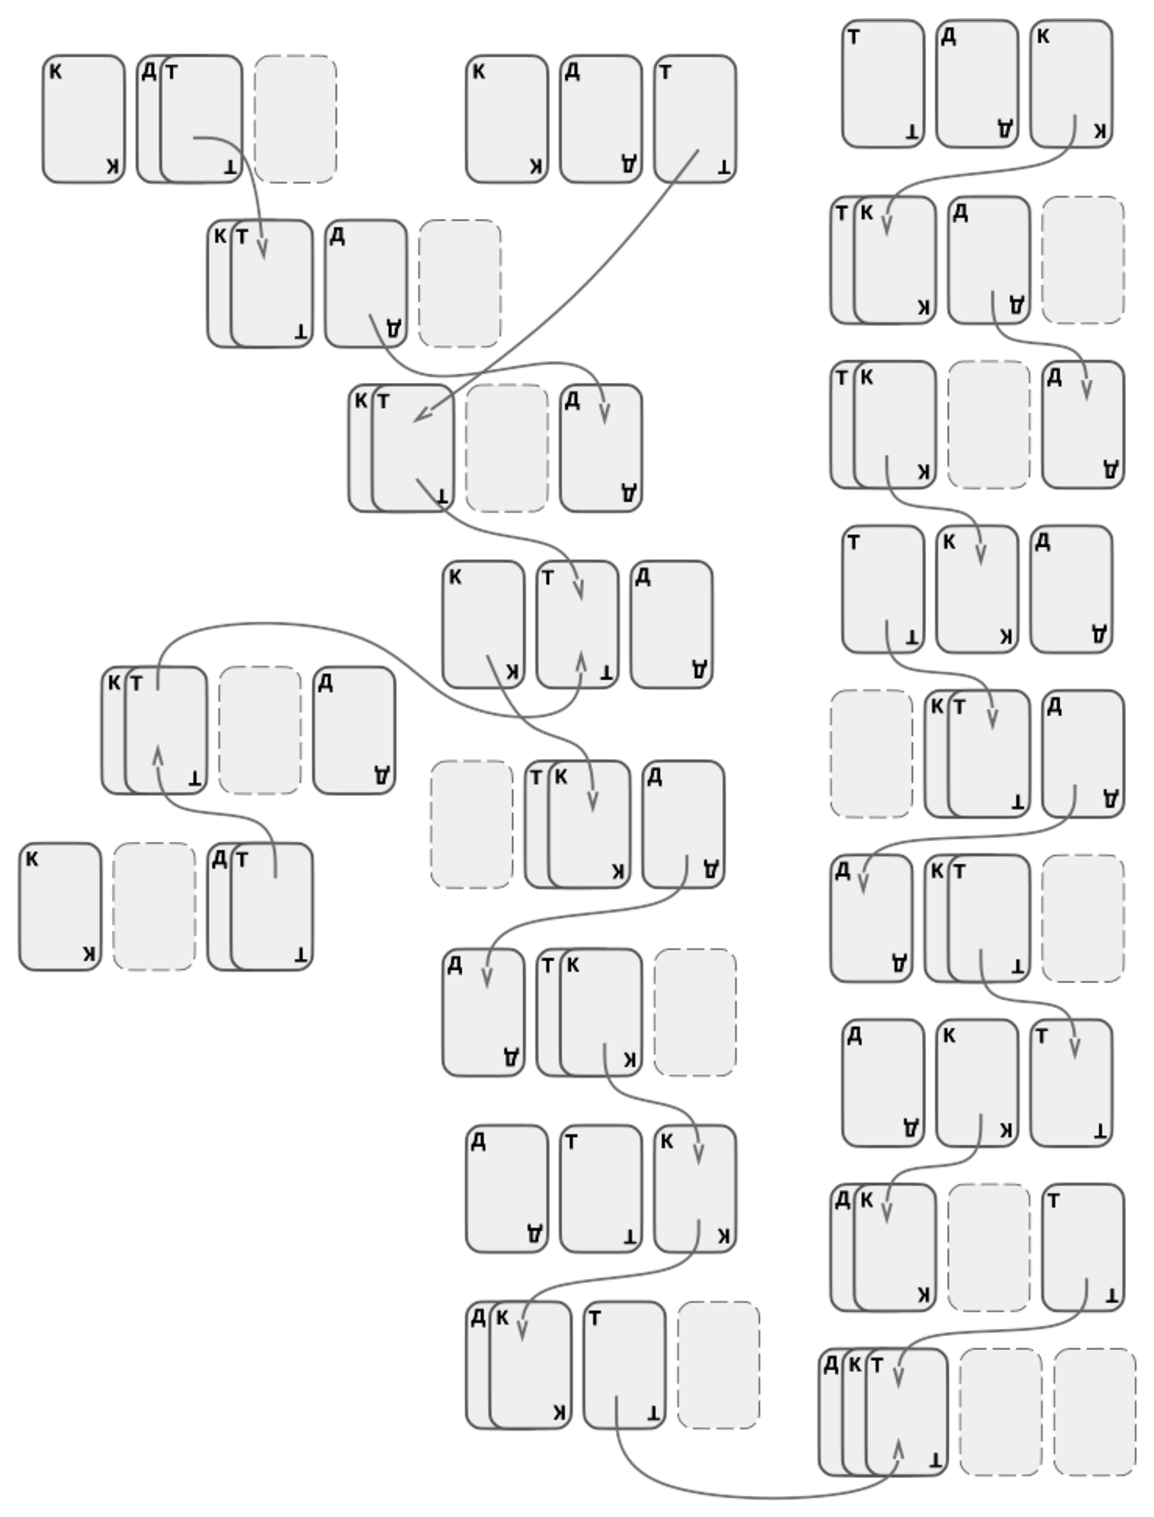
\includegraphics[scale=0.55]{Figs/Handicaps/conway-ru}
\end{figure}
Таким образом, достаточно проверить, что все шесть возможных комбинаций открытых карт приводят к победе  (см. диаграмму).
\heart

Удивительным образом, этот алгоритм можно обобщить для работы с любым (фиксированным, известным) числом карт, оперируя всё теми же тремя колодами.
Скажем, для 52 карт, пронумерованных от 1 до 52, следующие правила (данные в приоритетном порядке) в конечном итоге приведут к тому, что слева окажется колода, сложенная по-порядку с $1$-й картой наверху.

\begin{enumerate}[(1)]
\item Если видим 2, 1, ---, то кладём $1$-ю на $2$-ю;
\item Если видим две произвольные карты, ---, то перекладываем карту вправо (возможно по кругу) в пустую колоду;
\item Если видим $k$, $j$, $k-1$, при $j < k$, то кладём $(k-1)$-ю на $k$-ю;
\item Если видим только одну карту, то перекладываем карту налево;
\item Если видим три карты, то карту справа от наибольшей перекладываем дальше направо (возможно по кругу).
\end{enumerate}

Докажем, что этот алгоритм действительно работает.
Предположим, что мы видим карту 52 в средней или в правой колоде.
Тогда, следуя правилу (2) и (5), она в итоге окажется в левой колоде а все остальные карты попадут в среднюю.
По мере их перемещения вправо согласно правилу (2), карты $51, 50, 49, \dots, k$ будут складываться на $52$-ю согласно правилу (3) для некоторого $k < 52$, и средняя колода опустеет.
Разумеется, если $k = 1$, то задача решена --- последний ход сделан по правилу (1).
В противном же случае $k$-я карта переместится в среднюю колоду по правилу (2) и в правую по правилу (5), за ней аналогичным образом последует $(k+1)$-я, и так далее, пока в правой колоде не окажется 51 карта, верхние карты которой упорядочены от $51$-й до $k$-й.

Теперь $52$-я карта перекладывается в среднюю колоду,
а правая колода перекладывается в обратном порядке в левую.
Далее $52$-я карта передвигается в правую колоду, а левая колода перемещается в среднюю колоду, снова меняя порядок.
Наконец $52$-я карта перекладывается обратно в левую колоду.
В этот момент в средней колоде окажутся карты от $51$-й до $k$-й, с $51$-й наверху.
Дальше карты с $51$-й по $k$-ю перемещаются согласно правилу (2) направо и оказываются в левой колоде по правилу (3), до тех пор пока, опять, $k$-я, $(k+1)$-я, $\dots, 52$-я не попадут в левую колоду.

Правая колода сейчас пустая, следовательно, $(k-1)$-я карта находится где-то в средней.
Если она не в самом низу, то ей придётся перейти в левую колоду и процесс, описанный выше, повторится для некоторого $k'<k$.
Если же случилось, что $(k-1)$-я карта оказалась в самом низу, то она не попадёт влево (если только, она не $1$-я), потому что, когда она переместится вправо по правилу (5), средняя колода опустеет, и мы вынуждены применить правило (2) вместо (3).
Однако, в конце следующего цикла, в средней колоде будет обратный порядок, с картой $k-1$ наверху.
Отсюда следует, что значение $k$ уменьшается хотя бы каждый второй раз, как $52$-я карта попадает в пустую левую колоду.

Для завершения доказательства, нам осталось проверить, что в какой-то момент $52$-я карта появится на верху средней или правой колоды.
Очевидно, что в какой-то момент $52$-я появится на одной из колод;
предположим, что на левой.
Следуя правилу (3), она может собрать над собой $51$-ю, $50$-ю, $\z\dots, k$-ю, а остальные карты окажутся в средней и, возможно, в правой колоде.
Затем правила (2) и (5) опустошат среднюю колоду.
Далее $k$-я карта переместится в середину и потом вправо, затем, аналогично, $(k+1)$-я, и так далее (как и выше), пока $52$-я снова не окажется наверху, но на этот раз (после того, как $51$-я перешла в правую колоду) средняя колода будет пустая.
Значит $52$-я кладётся на среднюю, и мы получаем желаемую конфигурацию.

\subsubsection*{Крутящиеся выключатели}% (SPINNING SWITCHERS)

Эта задача попала ко мне от Саши Барга из Мэрилендского университета, но, похоже, что в этот момент она была уже много где известна.
Как и во многих других задачах, окажется полезным рассмотреть сначала более простой её вариант.

\medskip

Рассмотрим версию с двумя выключателями: нажав на обе кнопки, мы выясним, находились ли они в одинаковом состоянии, если да, то лампочка загорится (если она уже не горела).
В противном случае, на следующем шаге нажмём одну кнопку, после этого кнопки \emph{будут} в одинаковом состоянии, и в наихудшем случае нам придётся сделать ещё один шаг, нажав сразу обе кнопки, чтобы лампочка наконец зажглась.

Вернёмся к варианту с четырьмя лампочками.
Обозначим через 
А операцию, когда мы нажимаем все четыре кнопки, 
D --- диагональные кнопки, 
N --- соседние и 
S --- одну кнопку.
Тогда последовательность операций ADANASADAND включит лампочку максимум за 12 шагов.

В более общем виде для выключателей в углах $n=2^k$-угольника это можно проделать за $2^{n}-1$ шаг следующим образом.
Пусть $X\z=X_1,\dots,X_m$ шаги для $\tfrac n2=2^{k-1}$-угольника.
Составим из противоположных выключателей пары, если $X_i$ --- шаг для $\tfrac n2$-угольника, при котором нажимаются кнопки $i_1,\dots,i_j$, тогда пусть $X_i'$ будет шагом для $n$-угольника, при котором нажимаются кнопки $i_1,\dots,i_j$ и $i_1+\tfrac n2,\dots,i_j+\tfrac n2$.
Пусть $X'$ обозначает последовательность шагов $X_1',\dots,X_m'$.

Нам также необходим шаг $X_i''$ для $n$-угольника, при котором нажимаются только кнопки $i_1,\dots,i_j$.

Будем говорить про противополжную пару, что она «чётная», если оба выключателя включены или оба выключены.
Если все пары чётные, то последовательность шагов $X'$ включит лампочку.
Идея в том, чтобы посредством применения шагов $X_1''$, $X_2''$ и так далее, сделать все пары чётными, каждый раз проверяя при помощи $X'$, добились ли мы успеха.
Порядок шагов такой:
\begin{align*}
X_1',\dots,X_m';X_1'';X_1',\dots,X_m';X_2'';
\\
X_1',\dots,X_m';\dots,:X_m'';X_1',\dots,X_m',
\end{align*}
или, более компактно: $X';X_1'';X',X_2'';X';\dots,X_m'',X'$.
Всего получилось $(m+1)m+m=m(m+2)$ шагов.
Следовательно, если $f(n)$ означает число шагов, предпринятых для решения $n$-угольника, то 
$f(n)=f(\tfrac n2)(f(\tfrac n2)+2)$,
и поскольку $f(1)=2^1-1=1$, получаем, что $f(n)=2^n-1$ если $n$ степень двойки.

Эта последовательность действий работает, потому что шаги типа $X''$ работают на чётных/нечётных парах также, как и шаги типа $X$ работали на включённых/выключенных парах, и, между тем, шаги типа $X'$ абсолютно не влияют на конфигурацию чётных/нечётных пар.
\heart

С другой стороны, задача не разрешима, если $n$ не является степенью двойки, например, если $n=m2^k$, при нечётном $m>1$.
Для представления одновременно конфигурации выключателей (1 = «включён», 0 = «выключен») и операции (1 = «нажать», 0 = «не трогать») можно прибегнуть к бинарным векторам длины $n$.
Пусть $v$ такой вектор, обозначим через $v^i$ результат его вращения на $i$ шагов вправо.
Применение операции $w$ к конфигурации $v$ приведёт к конфигурации $v+w$, если поворота не было, но поскольку поворот был, мы получаем $v+w^i$ для некоторого значения $i$.

Будем говорить, что $n$-вектор $v$ является «неровным», % [rough ?], 
если число различных его вращений $v^0,v^1,\dots,v^{n-1}$ не равно степени двойки.
Предположим (как и в начале), что до применения операции возможна \emph{любая неровная конфигурация с точностью до вращения}.
Мы утверждаем, что после любой фиксированной операции $w$ все ещё возможна \emph{любая неровная конфигурация с точностью до вращения}.
Таким образом нет гарантированного способа избавится от неровных конфигураций и, в частности, нельзя гарантировать получения $11\dots1$.

Для нечётного $n$, то есть при $n=m$, все векторы, кроме $00\dots0$ и $11\dots1$ неровные.
Если $w$ некий вектор и $v$ неровный вектор, то $v-w$ (то же что и $v+w$), или $v-w^1$ будут неровными, так что, если одно из вращений векторов $v-w$ или $v-w^1$ было возможно до применения операции, то вращение $v$ возможно после её применения.

Если $n=m2^k$, при $k>1$, то можно разбить $n$-цикл на сегменты длины $2^k$; вектор $v$ будет неровным если только он не одинаков на всех сегментах.
Следовательно, если вектор $v$ неровный, то существует $1\le j\le 2^k$, что его координаты $i2^k+j$ для $1\le j\le m$ не все равны.
И остаётся применить рассуждение выше, к векторам $v-w$ и $v-w^{2^k}$.

\subsubsection*{Комната с одной лампочкой}% (THE ONE-BULB ROOM)

Я услышал эту задачу от Адама Чэлкрафта, %(Adam Chalcraft)
который имеет честь представлять Великобританию на международных соревнованиях по одноколёсному хоккею.
Задача также появлялась на сайте www.ibm.com и была перепечатана в Emissary --- информационном бюллетене Математического института в Беркли. %(Matematical Science Research Institute) 
Одна из версий задачи появлялась даже в заслуженно известной программе Национального Общественного Радио «Car Talk» в 2003 году.

Однако, считаю нужным предупредить читателя, что эту задачу иногда путают с куда более сложной задачей, с которой вам предстоит встретиться в следующей главе.

\medskip

Безусловно, необходимо предположить, что между посещениями заключённых никто в комнате с лампочкой не балуется.
Заключённым необязательно знать, в каком состоянии изначально находится лампочка.

Идея заключается в том, что один из заключённых (скажем, Алиса) всё время пытается лампочку включить, а каждый из остальных выключает её \emph{два раза}.

Более подробно: Алиса всегда включает лампочку, если она выключена, в противном случае, оставляет её включённой.
Остальные заключённые выключают её первые два раза, если она включена, и оставляют её гореть при последующих посещениях.

Алиса считает, сколько раз она попадает в тёмную комнату после своего первого 
посещения, после $2n-3$ \emph{тёмных} визитов, она может заключить, что все побывали в комнате.
И вот почему:
Каждое тёмное посещение говорит о том, что один из остальных $n-1$ заключённых побывал в комнате.
Если же кто-то из них, скажем, Боб, не посещал комнаты, то лампочка не могла быть выключена больше, чем $2(n-2)\z=2n-4$ раз.
С другой стороны, Алиса в конце концов должна будет достичь её $2n-3$ тёмных визитов, потому что в итоге лампочка будет выключена $2(n-1)\z=2n-2$
раз и только одно из этих выключений (в случае если один из заключённых побывал в комнате до первого визита Алисы и выключил изначально горящую лампочку) может не засчитаться Алисой за тёмный визит.

Если заключённых только два, то каждый из них узнаёт о том, побывал ли другой в комнате, поскольку Алиса дожидается её первого тёмного повторного посещения, в то время как Боб ждёт свой первый \emph{светлый} повторный визит.
Однако, для случая $n>2$ имеется доказательство того, что невозможно гарантировать, что более одного заключённого узнают посетили ли все остальные комнату.
Ниже приводится набросок этого доказательства.
Читателям рекомендуется его пропустить, если только им не интересно, как получаются отрицательные результаты в задачах о передаче информации.
Я включил это доказательство потому, что, насколько мне известно, оно нигде не появлялось.

По сути, мы утверждаем, что противник (который знает стратегию заключённых) может вынуждать их совершать только бесполезные действия, кроме тех, что применялись в протоколе выше.

Давайте сосредоточимся на одном заключённом, Алисе.
Мы предполагаем, что её стратегия детерминистическая и основана исключительно на последовательности состояний лампочки, которые она до сих пор наблюдала.

Предположим, что стратегия Алисы заставляет её (в некоторых обстоятельствах) изменить состояние лампочки, после того, как она нашла её в том же состоянии, что и во время своего последнего посещения.
Тогда противник может немедленно отправить её обратно в комнату, «сводя на нет» её предыдущий визит.
В результате, эта часть стратегии Алисы может только дать противнику дополнительную опцию.
Исходя из этого, можно предположить, что Алиса не должна менять состояние лампочки, если она находит её в том же виде, как оставила в свой последний визит.

Далее, предположим, что Алисе в некий момент требуется оставить лампочку в том же состоянии, в котором она её нашла.
Тогда мы утверждаем, что можно предположить, что после этого она никогда снова не предпримет каких-либо действий!
Почему?
Потому что, если противник не хочет, чтобы она продолжала действовать, то он может устроить так, что Алиса никогда не увидит лампочку в состоянии, отличном от того, которое она видит в данный момент.
Он может это сделать, поскольку, если Алиса действительно останется навсегда неактивной, то, по крайней мере, одно из состояний («включено» или «выключено») будет повторяться бесконечно часто.
Положим, это «выключено».
Тогда противник может составить расписание для Алисы так, что лампочка будет выключена как в её посещении сейчас, так и во всех последующих, и следовательно, согласно предыдущему рассуждению, она никогда не будет снова действовать.
Итак, ещё раз, в этом случае у противника есть возможность заставить Алису замолчать, и можно предположить, что ровно это он и делает.

Очевидно, Алиса не может начинать с инструкции оставить лампочку в том же состоянии, как она её находит, так как в этом случае она перестанет действовать совсем, и никто никогда не узнает, посещала ли она комнату.%
\footnote{Если только она не пользуется очень сильными духами...}
Скажем, она должна включить лампочку, если она выключена, в обратном случае оставить лампочку как есть.
Тогда она ничего не будет делать до тех пор, пока опять не попадёт в комнату с выключенной лампочкой, и в этом случае она может только снова включить лампочку или остаться бездейственной навсегда.
Таким образом, число раз, когда Алиса включает лампочку, ограничено неким $j$ (которое можно считать константой, иначе у противника будет больше преимуществ).
Назовём такую стратегию $+j$, где $j$ положительное целое число или бесконечность.
Аналогичное рассуждение, применённое для случая, когда Алиса должна во время первого визита выключить лампочку, приводит к стратегии $-j$.

Остаётся ещё один вариант, когда Алиса должна будет изменить состояние лампочки в свой первый визит в комнату, но в этом случае далее она вынуждена будет продолжить действовать так, как описано выше, в зависимости от того, включила она лампочку или выключила.
И это снова даёт противнику дополнительное преимущество.

Всё сводится к тому, что у каждого заключённого имеется стратегия $+j$ или $-j$ для различных $j$.
Если все они только выключают (или включают) лампочку, то никто ничего не сможет определить.
Таким образом, можно предположить, что у Алисы стратегия $+j$, а у Боба $-k$.
Если Чарли включает лампочку, Алиса никогда не сможет определить, закончили ли Боб или Чарли, или же у них остаётся ещё по одному заданию.
Если Чарли выключает лампочку, то тогда Боб --- это тот, кто останется в неведении.

Учитывая всё вышесказанное, мы получаем, что для того, чтобы какой-то заключённый смог определить, что все посетили комнату,
Алиса должна включать лампочку, в то время как все остальные выключать (или наоборот).
Действительно, если стратегия у Алисы $+j_1$, а у остальных  $-j_2,\dots,-j_n$, то легко проверить, что условие, при котором каждое $j_i$ конечно и не меньше 2, а $j_1$ больше, чем сумма остальных минус наименьший из них, является необходимым и достаточным.

Значит, если $n>2$, то максимум одному заключённому гарантирована честь знать, все ли побывали в комнате.
Уфф!

\subsubsection*{Два шерифа}% (ТHE TWO SHERIFFS)

Если два шерифа (назовём их Лев и Ральф) обменялись секретной информацией, то они смогли бы использовать этот секрет для того, чтобы зашифровать свой разговор и достичь цели.
Но так как они никогда прежде не встречались, им придётся \emph{изготовить} этот секрет.

\medskip

Предположим, что пары, к которым Лев и Ральф сузили свои списки подозреваемых, не одинаковы, то есть существует возможность определить убийцу.
В этом случае, если, скажем, Лев просто называет свою пару, то Ральф будет знать, кто убийца.
Но тогда и банда линчевателей будет знать всё, что знает Лев, так что любая попытка Ральфа сообщить Льву имя убийцы, без того, чтобы об этом не прознали линчеватели, обречена на провал.

Лев и Ральф должны подойти к определению имени убийцы более хитрым способом.
Составим таблицу из всех возможных пар подозреваемых таким образом, что каждый столбец содержит разбиение восьми подозреваемых на четыре пары.
Вот один из способов:

\[
\begin{matrix}
\{1,2\}&\{1,3\}&\{1,4\}&\{1,5\}&\{1,6\}&\{1,7\}&\{1,8\}
\\
\{3,4\}&\{2,4\}&\{2,3\}&\{2,6\}&\{2,5\}&\{2,8\}&\{2,7\}
\\
\{5,6\}&\{5,7\}&\{5,8\}&\{3,7\}&\{3,8\}&\{3,5\}&\{3,6\}
\\
\{7,8\}&\{6,8\}&\{6,7\}&\{4,8\}&\{4,7\}&\{4,6\}&\{4,5\}
\end{matrix}
\]


Лев и Ральф совершенно свободно могут обсуждать по телефону вопрос о сокрытии информации от линчевателей.
В частности, ничто не может помешать им согласиться пронумеровать подозреваемых и составить такую таблицу, как приведённая выше.

Далее Лев сообщает Ральфу, в каком столбце находится его пара.
Например, если пара Льва $\{1,2\}$, он говорит: «Моя пара в первом столбце.» 

Если пара Ральфа находится в том же столбце, он тут же понимает, что у него и Льва одинаковые пары.
Он может прямо сказать об этом, после чего шерифам остаётся только повесить трубки и вернуться к сыскной работе.

В противном случае Ральф понимает, что пара Льва одна из двух пар в столбце.
Вернёмся к нашему примеру, если пара Ральфа $\{2,3\}$, он знает, что у Льва должна быть пара $\{1,2\}$ или $\{3,4\}$.
Затем он разделяет столбец на две равные части, так, чтобы обе предполагаемые пары были в одной части, и сообщает об этом разбиении Льву.

В нашем примере он должен будет сказать Льву: «Моя пара либо в $\{1,2,3,4\}$, либо в $\{5,6,7,8\}$.» (Если же пара Ральфа была бы $\{2,5\}$, то он сказал бы: «Моя пара либо в $\{1,2,4,5\}$, либо в $\{3,4,7,8\}$.» )

Лев, безусловно, будет знать, в какой части надо искать пару Ральфа, так как она может быть только в той части, где находится его собственная пара.
Это и есть секрет Ральфа и Льва!

Теперь Лев может сказать Ральфу стоит ли его пара на первом или втором месте в соответствующей части.
Если, как в примере выше, пары $\{1,2\}$ и $\{2,3\}$, Лев может сказать: «Моя пара первая.», или, тоже самое, «Моя пара либо $\{1,2\}$, либо $\{5,6\}$.»

Далее, Ральфу становится ясно, какая пара у Льва, а, следовательно, и кто является убийцей.
Он может сообщить об этом Льву, просто сказав, что убийца  имеет больший или меньший номер в паре Льва.
То есть, он сказал бы: «Убийца --- второй в твоей паре.», или же: «Убийца --- 2 или 6.»

Банда линчевателей не сможет понять, о какой из «частей» говорят Лев и Ральф.
Если бы у Льва была пара $\{5,6\}$, а у Ральфа $\{6,7\}$ или $\{6,8\}$, то весь разговор, подслушанный линчевателями, был бы абсолютно таким же, как в рассмотренном примере, и в этом случае номер убийцы был бы 6, а не 2.
\heart
 
Задача была придумана как иллюстрация к идее, предложенной вашим автором лет двадцать пять тому назад:
а именно --- по открытым каналам связи из общеизвестной информации можно сделать общую тайну.%
\footnote{D.
Beaver, S. Haber, P. Winkler ``On the Isolation of a Common Secret''. \emph{The Mathematics of Paul Erd\H{o}s} Vol. II, R. L. Gracham and J.Nesetril, editors, Springer-Verlag, Berlin, 1996}
Первоначально эта идея применялась для игры в бридж, где партнёрам не разрешается иметь не объявленных договорённости о значениях заявок и игре.
С 1924 года, когда был создан современный бридж, считалось (неверно), что это правило препятствует какому-либо секретному общению между партнёрами.
Это заблуждение оказало весьма сдерживающий эффект на развитие более совершенных методов торговли и стратегии вистующих, так как многие считали, что такие методы могут давать противникам слишком много информации.
Например, основанная на научных методах шлемовая торговля подскажет противнику, с какой карты начинать.

Однако карты у вас в руке (которых, как вы знаете, нет у вашего партнёра) дают вам и вашему партнёру некое общее знание, которое может быть использовано для секретного общения.\footnote{
Подробную информацию и ссылки можно найти в статье P. Winkler ``The Advent of Cryptology in the Game of Bridge''. \emph{Cryptologia} Vol. 7 \#4 (October 1983), pp 327--332.}

\subsubsection*{Рассеянный профессор}% (THE ABSENT-MINDED PILL TAKER)

Профессорская коробочка для таблеток состоит из семи прозрачных ячеек, помеченных \textsc{вс}, \textsc{пн}, \textsc{вт}, \textsc{ср}, \textsc{чт}, \textsc{пт}, \textsc{сб} (см. рисунок ниже).
Представим, что профессор получает 30 новых таблеток в пятницу утром.
Он хочет распределить их по ячейкам таким образом, чтобы посмотрев на свою коробочку, начиная с этого дня, он мог бы сказать, выпил он свою ежедневную таблетку, и, если нет, то смог бы взять её из соответствующей ячейки.

Очевидный способ это сделать --- положить по 5 таблеток в \textsc{пт} и \textsc{сб} и по 4 таблетки в \textsc{вс}, \textsc{пн}, \textsc{вт}, \textsc{ср}, \textsc{чт} и следовать такому алгоритму:
\begin{itemize}
 \item[]
 Если в коробочке есть непрерывная по модулю 7 строка из ячеек с $k$ таблетками, а в остальных ячейках по $k-1$, то он знает, что самая левая «тяжёлая» ячейка (то есть с $k$ таблетками) --- это та, откуда нужно брать следующую таблетку.
Если это среда, и такая ячейка помечена \textsc{ср}, он берёт оттуда таблетку, если же эта ячейка \textsc{чт}, он знает, что таблетка уже принята.
\end{itemize}

Трудность заключается в том, что каждые семь дней все ячейки становятся равными, то есть, в каждой из них одно и тоже число таблеток.
Какую ячейку нужно тогда выбрать?
Ну, в данном случае, профессор понимает, что это случится в воскресенье, так что он устанавливает правило: если все ячейки равны, то надо брать из контрольного контейнера --- \textsc{вс}.
То есть, если он видит равные ячейки и этот день --- воскресенье, он берёт таблетку из \textsc{вс}, если же это суббота, значит, он уже таблетку принял.

Всё идёт прекрасно до тех пор, пока, 30 дней спустя, он получает новые 30 таблеток.
Это происходит в воскресенье, значит, он распределит таблетки по 5 штук в \textsc{сб} и \textsc{пн} и по 4 штуки в остальные ячейки;
тогда он видит, что ячейки станут равными во вторник утром, а не утром в воскресенье.
Это катастрофа --- профессор не в состоянии запомнить, что контрольный контейнер теперь \textsc{вт}, а не \textsc{вс}.

Определённо, существует решение этой задачи, которое не вынуждает оставлять таблетки в банке (или выбрасывать их).
Но какое? Профессору нужен надёжный способ отмечать ячейку, из которой нужно взять следующую таблетку.
Он мог бы положить значительно большое количество таблеток в одну ячейку и затем передвигать эту «кучу» каждый день, но, как мы знаем, в этом случае он не будет уверен, что уже переложил кучу.
Так или иначе профессору нужно придумать простой алгоритм, который позволит ему принимать свою ежедневную таблетку, не перекладывая остальные.

Разумеется, профессор начинает задаваться вопросом, а существует ли у этой задачи решение;
может удастся доказать его невозможность?
Если каждый день он берёт таблетку из ячейки, помеченной только этим днём, то, пойдя в обратную сторону от последней таблетки, мы видим, что каждый день коробочка состоит либо из равных ячеек, либо из непрерывной строки ячеек с $k$ таблетками и остатка ячеек с $k-1$ таблетками.
Таким образом, он приходит назад к начальной задаче, где необходимо менять и запоминать контрольную ячейку.

Но подождите, а есть ли причина почему, скажем, в среду он должен брать таблетку именно из ячейки \textsc{ср}? Вовсе, нет.
Конечно, алгоритм должен оставаться простым, иначе можно перегрузить даже долговременную память профессора.
То есть можно допустить эту дополнительную свободу при условии, что есть разумное правило для выбора ячейки, из которой нужно взять таблетку (а также для определения не была ли она уже взята).

Оказывается, существует алгоритм, отвечающий всем требованиям профессора и допускающий только одно небольшое исключение из того, что таблетка всегда берётся из ячейки, соответствующей текущему дню недели.
Профессор рассуждает следующим образом:

\begin{enumerate}[(1)]
\item Таблетки следует распределять по ячейкам \emph{более-менее} поровну.
Иначе возникнут неудобства в конце, перед покупкой новой упаковки.
\item Необходимо избегать \emph{полностью} равного распределения, иначе опять возникнет проблема с определением «контрольного контейнера».
\item В силу (2), не всегда может быть правильным выбирать ячейку с наибольшим количеством таблеток.
\end{enumerate}

Учитывая эти условия, профессор приходит к идее, что в любой момент должно иметься не более трёх размеров ячеек, и что, если возможно, он должен брать таблетку из ячейки среднего размера.
Чтобы сделать это как можно проще, будем считать, что есть только одна «куча» --- ячейка, с наибольшим числом таблеток.
Обозначим через $k$ число таблеток в куче в любой день.
Во всех остальных ячейках будет $k-1$ или $k-2$ таблеток, и те ячейки, в которых $k-2$, будут непрерывной строкой справа от кучи.
На рисунке ниже представлены несколько допустимых конфигураций.

\begin{figure}[h!]
\centering
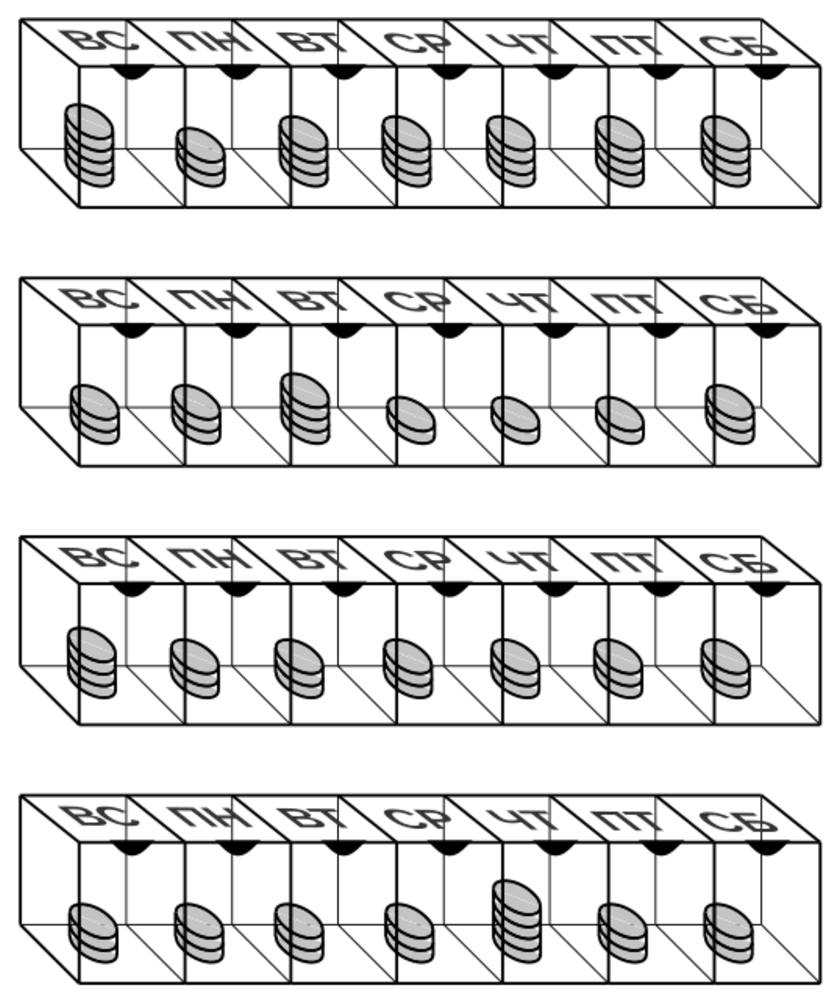
\includegraphics[scale=0.5]{Figs/Handicaps/box1-ru}
\end{figure}

Первая ячейка вправо от кучи, содержащая $k-1$ таблеток, будет той, из которой нужно взять таблетку.
Если ячейки с $k-1$ таблетками нет, то надо брать таблетку из кучи.
В почти всех случаях надпись на ячейке, из которой берётся таблетка, правильная, то есть совпадает с текущим днём недели.

Например, коробочки на рисунке выше подготовлены для приёма таблетки во вторник, субботу, понедельник и четверг, соответственно.

Исключением является момент, когда у профессора остаётся последняя таблетка.
В предыдущий день он обнаружил две оставшиеся таблетки вместе в ячейке, помеченной соответствующим днём недели, и он одну оттуда взял (согласно правилу, надо брать из кучи если нет ячейки размером на один меньше, чем куча).
Теперь последняя таблетка лежит в ячейке, помеченной \emph{вчерашним} днём, и эту таблетку он принимает сегодня.

Легко заметить, что если таблетки разложены должным образом, то правила соблюдаются до последней таблетки.
Но всегда ли возможно всё правильно настроить, когда приходят новые таблетки?
И да, действительно, существует единственная правильная конфигурация для любого данного числа таблеток и любого данного дня недели, то есть ровно так профессору следует раскладывать новые таблетки.
Профессор вычисляет день, когда должна быть принята последняя таблетка (а именно, вчерашний день недели плюс число таблеток по модулю 7,
предполагается, что сегодняшнюю таблетку он ещё не выпил).
Конечно, дни недели пронумерованы последовательно  по модулю 7, но не имеет значения, который день номер~1.

Если, скажем, в среду утром пришло 32 таблетки, то профессор знает, что последнюю таблетку надо будет принять в субботу (из ячейки \textsc{пт}!) Из этого следует, что ячейка \textsc{пт} содержит кучу.
Профессор кладёт шесть таблеток в \textsc{пт}, по четыре таблетки в \textsc{сб}, \textsc{вс}, \textsc{пн}, \textsc{вт}, и по пять в \textsc{ср} и \textsc{чт}.
И теперь у него всё устроено должным образом, чтобы принять таблетку за среду.
\heart

Уместно спросить:
«А что, если у нас меньше, чем семь ячеек?
При каком наименьшем числе ячеек наша задача имеет решение?
А что, если в неделе $d$ дней, вместо семи,
каково тогда наименьшее возможное число ячеек, как функция от $d$?»

Отметим, что профессорское решение работает и на Юпитере, где в неделе $d$ дней ($d>1$), и где коробочки для таблеток, конечно же, имеют $d$ ячеек.
В случае $d=2$ это сводится к тому, что в одной ячейке держится на одну или две таблетки больше.
Решение для двух ячеек может быть использовано для любого чётного $d$, так как человек, принимающий таблетки, знает, какой сейчас день этой чётной недели, а значит он знает и чётность этого дня.
Так что наличие двух ячеек достаточно и, конечно, необходимо, если $d$ чётно.

Однако, две ячейки не сработают, если $d$ нечётно.
В этом случае непременно найдутся два последовательных дня недели, которые должны сойтись к одной однотаблеточной конфигурации, так что, когда человек видит такую конфигурацию в первый из этих дней, он не может сказать, принял ли он таблетку в этот день или нет.

Читателю, прошедшему уже такой долгий путь, не составит труда убедить себя, что при нечётных $d$ достаточно трёх ячеек.
Но придумать простой алгоритм с тремя ячейками для семидневной недели довольно сложно.
Предложенная далее схема основана не мнемоническом использовании двоичной записи.

Пронумеруем дни недели, начиная с воскресенья = 1 и заканчивая субботой = 7, числами по модулю 7.
Схема включает в себя семь «типов конфигураций», пронумерованных от 1 до 7, а конфигурации в каждом типе определяются по бинарному представлению номера типа.
При этом мы считаем, что ячейки располагаются в линейном порядке --- «левая», «центральная» и «правая» (то есть циклический порядок использоваться не будет).

Так, например, тип $1=001_2$ требует, чтобы правая ячейка была задействована как куча с гораздо б\'{о}льшим количеством таблеток, чем будет в каждой из двух остальных.
Тип $3 = 011_2$ требует, чтобы в левой ячейке было существенно меньше таблеток, чем в любой из двух остальных ячеек,
а тип 7$ = 111_2$ --- чтобы ячейки были более-менее равными.

Точнее, типы 1, 2 и 4 имеют кучи (справа, в центре и слева, соответственно), в которых на две или три таблетки больше, чем в любой из двух других ячеек.
При этом оставшиеся две ячейки, если они различны, то упорядочены так, что б\'{о}льшая ячейка находится правее.

Далее, типы 3, 5 и 6 имеют особую наименьшую ячейку слева, в центре или справа, соответственно.
Две другие ячейки содержат каждая на две таблетки больше, если они одинаковые.
Если нет, то они различаются по размеру не больше, чем на одну таблетку, и б\'{о}льшая ячейка расположена правее и содержит на 2 или 3 таблетки больше, чем самая маленькая.

Тип 7 требует, чтобы содержимое ячеек отличалось друг от друга максимум на одну таблетку, с меньшими ячейками справа (см. таблицу).

Теперь стратегия: если в день $D$ получено $P$ таблеток, то они распределяются согласно типу $P+D \pmod 7$.
Таблетки берутся так, чтобы сохранялся тип.

В частности, каждый день, профессор, смотрит на тип $T$ и поступает следующим образом:
если в день $D$ он видит $P>3$ таблеток и $D+P\ne T\pmod 7$, значит, он уже в этот день таблетку принял.
В противном случае, он берёт таблетку из одной ячейки, так, чтобы сохранить тип конфигурации.

\begin{center}
  \begin{tabular}{ l | c c c c }
     & 3 таб. & 4 таб & 5 таб & 6 таб \\ \hline
    тип 1 & 003 & 013 & 113 & 114 \\ 
    тип 2 & 030 & 031 & 131 & 141 \\ 
    тип 3 & 012 & 022 & 023 & 123\\ 
    тип 4 & 300 & 301 & 311 & 411\\ 
    тип 5 & 102 & 202 & 203 & 213\\ 
    тип 6 & 120 & 220 & 230 & 231\\ 
    тип 7 & 111 & 211 & 221 & 222
  \end{tabular}
\end{center}

Когда же останется три таблетки или меньше, становится трудно следовать какому-либо типу, но можно воспользоваться правилом «слева-направо» для типов, чтобы решать, как необходимо менять дальше конфигурации.
Это сводится к использованию следующей таблицы:

\begin{figure}[h!]
\centering
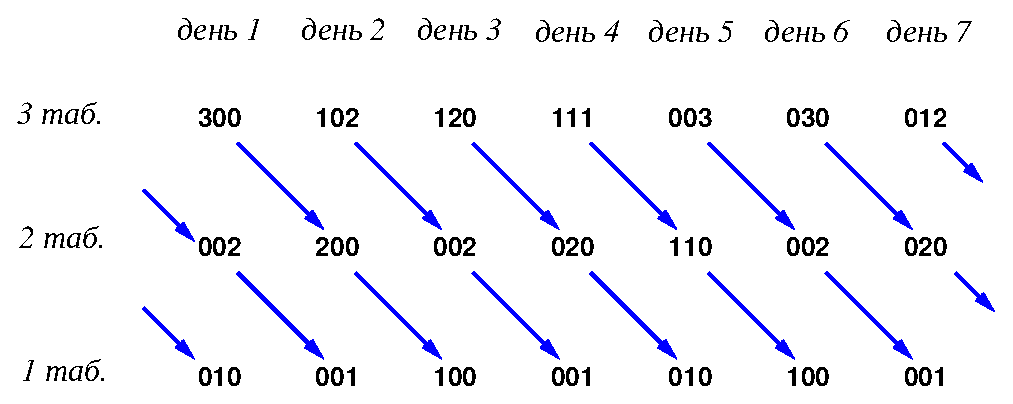
\includegraphics[scale=0.6]{Figs/Handicaps/3box-ru}
\end{figure}

Чтобы воспользоваться таблицей, нужно найти в ней запись, соответствующую $D$ и $P$;
если такая имеется, то нужно взять таблетку так, чтобы после получилась конфигурация ниже и направо (следуя по диагонали).
В противном случае, конфигурация будет соответствовать дню $D+1$, и, значит, таблетка за этот день уже принята.

\chapter*{Крепкие орешки}
\addcontentsline{toc}{chapter}{Крепкие орешки}

\setlength{\epigraphwidth}{.6\textwidth}
\epigraph{Задай  труднейший  из  вопросов!  и  смотри...\\
Ответ  прекрасный  возродится  изнутри!}{---Мавлана Джалал ад-Дин Мухаммад Руми «Радость   при   неожиданном разочаровании»
}

Задачи этого раздела сложны, но ст\'{о}ят потраченных усилий.
Некоторые из них являются вариациями или продолжениями уже рассмотренных задач.

\medskip

Следующая задача была сформулирована
Китом Кёрнесом %K. A. Kearnes
и Эмилем Киссом.%Emil Kiss
\footnote{K. Kearnes, E. Kiss, ``Finite algebras of finite complexity''. \emph{Discrete Math.} 207 (1999), no. 1-3, 89--135.}
Петар Маркович привёз эту задачу на конференцию в честь Даниила Клейтмана, проходивщей в Массачусетском технологическом институте в 1999 году.
Нога Алан, Том Боуман, Рон Хольцман и сам Даниил Клейтман решили её на той же конференции.

Конечно же, и эту задачу ст\'{о}ит попробовать решить самостоятельно, но не стоит расстраиваться, если не получится.

\subsection*{Ящики с подъящиками}
\rindex{Ящики с подъящиками}

Зафиксируем положительное целое число $n$.
\emph{Ящиком} будем называть декартово произведение $n$ множеств;
если даны $n$ множеств $A_1,\dots,A_n$, то их ящик $A_1{\times}\dots{\times}A_n$ есть множество всех последовательностей $a_1,\dots,a_n$ таких,
что $a_i$ лежит в $A_i$ для каждого~$i$.

Ящик $\bm{B}=B_1{\times}\dots{\times}B_n$ называется \emph{подъящиком} $\bm{A}=A_1{\times}\z\dots{\times}A_n$ если $B_i$ является собственным подмножеством $A_i$ для каждого~$i$.

Возможно ли разбить какой-нибудь ящик на менее чем $2^n$ подъящиков?

\paragraph{Решение:} Найти разбиение на $2^n$ подъящиков легко если конечно каждое множество $A_i$ имеет хотя бы два элемента.
Однако никто не смог обойтись меньшим числом; ниже будет показано, что это сделать невозможно.

Рассмотрим один из сомножителей $A_i$. 
Выберем в нём собственное подмножество $B_i$.
Выберем в $A_i$ случайное подмножество $C_i$ с нечётным числом элементов ($C_i$ может совпасть с $A_i$ если $|A_i|$ нечётно).

Заметим, что вероятность того, что $|C_i\cap B_i|$ нечётно равна $\tfrac12$.
Действительно, 
$C_i$ можно получить выбирая элементы $A_i$ по порядку так, чтобы предпоследний элемент лежал в $B_i$, а последний в его дополнении $A_i\backslash B_i$.
Каждый раз решение можно принимать подбрасывая монетку и только последний элемент следует выбрать так чтобы число $|C_i|$ получилось нечётным.
В этом случае последний бросок монеты определяет чётность $|C_i\cap B_i|$.

Заметим, что ящик $\bm{C}=C_1{\times}\dots{\times}C_n$ имеет нечётный размер тогда и только тогда, когда $|C_i|$ нечётно для каждого~$i$.
Пусть $\bm{C}=C_1{\times}\dots{\times}C_n$ есть случайный ящик нечётного размера в $\bm{A}$, то есть $C_i\subset A_i$ для каждого~$i$.
В этом случае вероятность того, что данный подъящик $\bm{B}=B_1{\times}\dots{\times}B_n$ пересекается с $\bm{C}$ по нечётному числу элементов равна $\tfrac1{2^n}$.

Предположим теперь, что существует разбиение на менее чем $2^n$ подъящиков $\bm{B}(1),\dots,\bm{B}(m)$.
Заметим, что вероятность того, что $\bm{C}$ пересекается с каждым подъящиком $\bm{B}(i)$ по чётному числу элементов положительна (она не меньше чем $1-\tfrac{m}{2^n}$),
но это невозможно, поскольку $\bm{C}$ содержит нечётное число элементов.
\heart

Для тех отважных сердец, что всё ещё с нами, мы предлагаем больше таких задач.
Начнём с задачи Сары Робинсон, которая попала в «Нью-Йорк таймс».\footnote{S. Robinson ``Why Mathematicians Now Care about their Hat Color''. \emph{The New York Times}, April 10, 2001.}

\subsection*{Отгадать цвет шляп}
\rindex{Отгадать цвет шляп}

Команда шляпников вернулась.

На этот раз цвет шляпы каждого игрока определяется подбрасыванием монеты.
Игроки становятся в круг так чтобы видеть цвета шляп остальных, никакого общения не допускается.
Далее игроков отводят в сторону и предоставляют шанс отгадать цвет своей шляпы --- он может быть синим или красным;
но им также предоставляется право \emph{молчать}.

Развязка ужасна: если все молчали или хотя бы один назвал неверный цвет, то всех игроков казнят.
Может показаться, что лучшей стратегией будет молчать всем, кроме одного, в этом случае шансы выжить будут $50\%$.
Но, поразительным образом, 15 игроков могут добиться выживания в более чем $90\%$ случаев. 
Как это сделать?

Если вам кажется, что улучшить шансы в $50\%$ невозможно, то скорее всего вы правильно поняли условие задачи.
Но прежде чем отчаиваться, попробуйте случай трёх игроков.

\medskip 

Решение следующей задачи неожиданно связано с решением предыдущей.
Далее подсказок не ждите.

\subsection*{Пятнадцать битов и шпионка}
\rindex{Пятнадцать битов и шпионка}

Каждый день шпионка имеет доступ к 15 битам на местной радиостанции.
Она не знает, как выбираются биты, но каждый день у неё есть возможность \emph{подменить} любой из них, поменяв его с 0 на 1 или наоборот.
После этого биты идут в эфир. 
Это единственный канал общения шпионки с центром.

Сколько информации она может передать за день?

\subsection*{Углы в пространстве}
\rindex{Углы в пространстве}

Докажите, что среди любого множества из более чем $2^n$ точек в $\mathbb{R}^n$, найдутся три, которые определяют тупой угол.

\subsection*{Два монаха на горе}
\rindex{Два монаха на горе}

Помните монаха из Главы 5 (Геометрия), который забрался на Фудзияму в понедельник, а спустился во вторник?
На этот раз он вместе с собратом-монахом поднимается на гору в один и тот же день, начиная одновременно с одной высоты, но по разным тропам.
По пути к вершине их тропы могут идти вверх и вниз, но не опускаются ниже стартовой высоты.

Требуется доказать, что монахи могут изменять свои скорости (возможно идя назад) так, чтобы в \emph{каждый} момент дня они находились бы на одной высоте!

\subsection*{Сумма под контролем}
\rindex{Сумма под контролем}

Дан список из $n$ вещественных чисел $x_1,\dots,x_n$ из отрезка $[0,1]$.
Докажите, что можно найти числа $y_1,\dots,y_n$ такие, что для любого $k$ выполняется $|y_k|=x_k$ и
\[\left|\sum_{i=1}^ky_i-\sum_{i=k+1}^ny_i\right|\le 2.\]

\subsection*{Двухламповая комната}
\rindex{Двухламповая комната}

Вы помните заключённых и комнату с одной лампой?
Теперь снова каждого из $n$ заключенных будут вызывать по одиночке на допрос, бесконечное число раз и в произвольном порядке, определяемом их тюремщиком.
Однако на этот раз в комнате для допроса есть \emph{две} лампы, каждая со своим бинарным переключателем.
Средств связи, кроме этих выключателей нет, и начальные состояния их неизвестны.
У заключенных снова есть возможность договориться заранее.

Опять же, требуется, чтобы один из заключенных в какой-то момент смог сделать вывод, что допросили всех.
Вы говорите, что это \emph{уже} сделано с \emph{одним} переключателем.
Да, но на этот раз требуется, чтобы все заключённые получили одинаковые инструкции.

\subsection*{Площадь и диаметр}
\rindex{Площадь и диаметр}

Докажите, что среди всех плоских фигур единичного диаметра, круг имеет наибольшую площадь.

\subsection*{Разрез пополам}
\rindex{Разрез пополам}

Докажите, что из каждого набора из $2n$ целых чисел, можно выбрать $n$ чисел, сумма которых делится на $n$.

\subsection*{Салфетки при случайном рассаживании}
\rindex{Салфетки при случайном рассаживании}

Помните задачу про банкет, там, где куча математиков рассаживается за большой круглый стол?
И снова, на столе, между каждой парой приборов, находится кофейная чашка с салфеткой.
Каждый человек, садясь, берёт салфетку слева или справа;
если обе в наличии, то он выбирает её случайным образом.

На этот раз метрдотеля нет; места занимаются в случайном порядке.
Предполагая, что число математиков велико, какая их доля (асимптотически) останется без салфеток?

\subsection*{Группа солдат в поле}
\rindex{Группа солдат в поле}

Возможно, вы также помните солдат в поле, каждый из них присматривал за ближайшим соседом.
Предположим большое число солдат стоят в случайных позициях на большом квадрате, и они разбиты на максимально возможное число групп таких, что солдаты присматривают только внутри групп.

Чему равен средний размер группы?

\subsection*{Игреки на плоскости}
\rindex{Игреки на плоскости}

Вам уже известно, что на плоскости нет несчётного числа непересекающихся топологических восьмёрок.
Конечно же, можно найти континуум отрезков и окружностей.
Закономерный вопрос: что можно сказать про игреки, то есть про подмножества топологически эквивалентные трём отрезкам с общим концом?

Докажите, что на плоскости можно нарисовать только счётное число непересекающихся игреков.

\subsection*{Снова намагниченные доллары}
\rindex{Снова намагниченные доллары}

В последней задаче мы возвращаемся к намагниченным долларам, но слегка увеличиваем их притяжение.
На этот раз бесконечная последовательность монет сыпется в две урны.
Когда одна урна содержит $x$ монет, а другая $y$, следующая монета попадет в первую урну с вероятностью $x^{1{,}01}/(x^{1{,}01}+y^{1{,}01})$, а иначе во вторую.

Докажите, что с какого-то момента одна из урн не получит ни одной монеты.

\section*{Решения и комментарии}

\subsubsection*{Отгадать цвет шляп}

Как мы предупреждали, случай трёх игроков помогает найти решение.
Как минимум, он даёт возможность убедиться, что $50\%$ можно улучшить.
Однако получить отсюда общий случай непросто.

Каждого из трёх игроков следует проинструктировать молчать если он видит шляпы разных цветов,
а если обе шляпы одного цвета, то называть цвет который он \emph{не видит}.
В случае если есть шляпы обоих цветов (а это шесть из восьми случаев), один назовёт правильный цвет, а два других промолчат.
В результате игроки выигрывают с вероятностью $75\%$.

Заметим, что в плохих случаях, когда все шляпы одного цвета, \emph{все три} игрока называют неправильный цвет.
То есть данный протокол упаковывает 6 неправильных ответов в две конфигурации, и это имеет решающее значение.
Ведь в среднем по всем конфигурациям, ровно половина угадываний должна быть верной, поэтому, чтобы выиграть, следует экономно использовать правильные угадывания, а неправильные паковать вместе.
Протокол для трёх игроков делает это наилучшим образом, и, значит, он является оптимальным.

Для $n$ игроков было бы идеально сделать тот же самое,
то есть построить два типа конфигураций: «хорошие», где ровно один угадывает правильно, и «плохие», в которых угадывают все, и все неправильно.
В этом случае хороших конфигураций будет в $n$ раз больше плохих,
что даст неплохую вероятность выигрыша, равную $n/(n+1)$.

Такую оптимальную вероятность возможно достичь только, если число всех конфигураций, $2^n$, делится на $n+1$;
то есть, если $n$ равно степени двойки без единицы.
Удивительным образом, это условие также является достаточным.

Ключ к протоколу состоит в разбиении конфигураций на плохие и хорошие так, что любая хорошая \emph{соседствует} ровно с одной плохой (две конфигурации соседствуют, если одну можно получить из другой, поменяв цвет одной шляпы).
И такой способ есть!

Пусть $n=2^k-1$.
Пронумеруем игроков $k$-значным не нулевым кодом в двоичной системе.
(Например, если $n=15$, то игроки нумеруются $0001,0010,0011,\dots,1110,1111$.)
Эти коды будем складывать как ним-числа%
\footnote{Названные так из-за их игры Ним.
Насколько нам известно, этот неожиданный термин появляется впервые на с. 43 в «Winning Ways».}, то есть без учёта переноса разрядов;
например, $1011 + 1101 =0110$, и ним-сумма любого кода с собой равна $0000$.

Плохими конфигурациями будут те, для которых ним-сумма кодов всех игроков с красными шляпами равна $0000$.
Стратегия состоит в следующем:
каждый игрок считает ним-сумму кодов всех, кого видит в красных шляпах.
Если ним-сумма равна $0000$, то он говорит, что у него красная шляпа.
Если же ним-сумма равна его коду, он говорит, что у него синяя шляпа.
В остальных случаях он молчит.

А почему это работает?
Предположим, что ним-сумма кодов \emph{всех} игроков с красными шляпами равна $0000$.
Тогда для каждого игрока с синей шляпой посчитанная им ним-сумма будет $0000$, и он скажет, что у него красная шляпа;
ним-сумма посчитанная каждым игроком с красной шляпой, будет его кодом, и он скажет, что у него синяя шляпа.
То есть каждый назовёт цвет, и каждый сделает это неправильно --- ровно то, что мы хотели!

Теперь  предположим, что эта ним-сумма равна чему-то другому, например, $0101$.
Тогда цвет назовёт единственный игрок с кодом  $0101$, и назовёт он его \emph{правильно}.

Ним-сумма равна $0000$ с вероятностью $1/16$ (поскольку имеется 16 различных ним-сумм).
Значит, вероятность выигрыша составит $15/16$;
в общем случае она равна $1-2^{-k}$.
Полезно проверить, что в случае $k=2$ мы получим наше решение для трёх игроков.

Если $n$ не степень двойки без единицы, то самое простое --- найти наибольшее $m<n$ вида $2^k-1$.
Эти $m$ игроков следуют описанной стратегии, а все остальные молчат независимо от того, что они видят.
В худшем случае (если $n=2^k-2$, при некотором $k$) вероятность выигрыша равна $(n/2)/((n/2)-1)$.
Вообще говоря, такая стратегия не самая лучшая;
при $n=4$ невозможно улучшить $75\%$, но при $n=5$ (как указал Элвин Берлекэмп) можно добиться вероятности $25/32>78\%$.
В общем случае наилучшая стратегия неизвестна.
\heart

Построенное нами множество плохих конфигураций не только красиво, но и полезно.
Оно называется кодом Хэмминга и является примером идеального самокорректирующегося кода.
Представьте, что вам надо посылать несколько битов информации по не очень надёжному каналу, который иногда переворачивает бит.
Сгруппируйте биты в строчки по 11 в каждой.
Существует $2^{15}/16\z=2^{11}$ красносиних строк длины 15 с ним-суммой $0000$;
их можно записать двоичным кодом (например, код $101010101010101$ значит, что все нечётные шляпы --- красные).
Эти 15-значные строки будут называться «допустимыми».
Поскольку число допустимых строк равно $2^{11}$, можно выбрать одну для каждой из 11-значных строк.
Простейший способ это сделать --- выбросить последние 4 бита из 15-значной строки.

Чтобы послать строку из 11 битов, вы посылаете единственную соответственную ей допустимую строку из 15 битов.
Вы проигрываете в скорости, но взамен получаете надёжность.
Действительно, если один из битов по ошибке перевернулся, то получающая сторона сможет узнать номер этого бита и перевернуть его назад!

Как? А надо взять ним-сумму кодов красных битов (тех, что соответствуют единицам) в полученной 15-значной строке и удостоверится, что она равна $0000$.
Пусть нет, скажем, она равна $0101$,
тогда какой-то бит перевернулся;
если это случилось только раз, то это должен быть пятый бит.
Значит, следует перевернуть пятый бит и сверится с системой кодов, чтобы понять, какая 11-значная строка соответствует полученной 15-значной.
Результат будет верен, если только не случилось нескольких переворотов зараз.

\medskip

Эта задача (в несколько другой формулировке) и её решение рассматривалась Тоддом Эбертом (сейчас в Калифорнийском университете в Ирвайне) в его диссертации, защищённой в 1998 в Калифорнийском университете в Санта-Барбаре.
Решение с кодом Хэмминга было предложено несколько лет до этого Стивеном Рудичем из Университета Карнеги — Меллона  для похожей задачи про выборы.

\subsection*{15 битов и шпионка}

Поскольку шпионка может произвести всего 16 действий (изменить какой-то бит или никакого), то она \emph{в принципе} может передавать четыре бита информации ежедневно.
Но как?

Ответить на это просто, если воспользоваться ним-суммами из предыдущего решения.
Шпионка и её центр присваивают $k$-тому биту 4-значный код, соответствующий числу $k$, а «сообщение» определяется как, ним-сумма кодов с единицами в передаче на радио.

Утверждение состоит в том, что шпионка может передать любое из 16 возможных сообщений по её желанию,
достигая таким образом, четырёх битов информации.
Предположим, она желает послать код $n$, а ним-сумма кодов с единицей в намеченной передаче равна $m\ne n$.
Тогда ей следует поменять бит номером, равным ним-сумме $m+n$.
Не имеет значения, был ли этот бит 0 или 1, так как ним-сумма равна ним-разности.
\heart

\medskip

Я узнал эту задачу от Ласло Ловаса из Microsoft Research, который не смог с уверенностью назвать её источник.

\subsubsection*{Углы в пространстве}

Мне дали эту задачу при собеседовании в Массачусетском технологическом институте, и я на ней засыпался.
Кажется, что $2^n$ вершин куба дают наибольшее число точек в $n$-мерном пространстве без тупого угла.
Но как это доказать?
Оказывается, этот вопрос был сформулирован Палом Эрдёшем и Виктором Кли и решён Людвигом Данцером и Бранко Грюнбаумом. %реф

\medskip

Пусть $x_1,\dots,x_k$ --- это различные точки (векторы) в $\mathbb{R}^n$, и пусть $P$ --- их выпуклая оболочка.
Можно предположить, что $P$ имеет объём 1;
этого можно добиться, уменьшив размерность пространства до размерности $P$, а затем подобрав подходящий масштаб.
Можно также предположить, что $x_1$ является началом координат (нуль-вектором).
Если эти точки не образуют тупых углов, то для каждого $i>1$ внутренность сдвига $P+x_i$ не перекрывается с внутренностью $P$;
это верно, поскольку плоскость через $x_i$, перпендикулярная вектору $x_i$, разделяет эти два многогранника.

Кроме того, внутренности $P+x_i$ и $P+x_j$ также не перекрываются при $i\ne j$;
они разделяются плоскостью через $x_i+x_j$, перпендикулярной к $x_i-x_j$.
Отсюда делаем вывод, что объём объединения $P+x_i$ для $1 \le i \le k$ равен $k$.
Однако все эти многогранники лежат внутри удвоенного многогранника $2P = P+P$, объём которого равен $2^n$. Следовательно, $k \le 2^n$, что и требовалось!
\heart

\subsubsection*{Два монаха на горе}

Давайте разделим каждый путь на монотонные «отрезки», в пределах которых путь всегда восходящий, или всегда нисходящий.
\footnote{Естественно предположить, что существует только конечное число монотонных отрезков, ведь нет смысла рассматривать отрезки существенно короче чем шаг монаха.
Однако если этого не предполагать, то ответ в задаче окажется другим.
%It's reasonable to assume there are only finitely many monotonic segments; it doesn't make sense for a segment to bemuch shorter than a monk's step size. However, if we do not assume that, then the answer to the puzzle will be different.
}
(Отрезки, идущие по одному уровню, не вызывают проблем, так как один монах может стоять и ждать, пока другой проходит такой отрезок).
Можно предположить, что каждый такой отрезок является прямым восхождением или спуском, так как мы можем заставить монахов варьировать скорости так, чтобы их скорость восхождения или спуска была постоянной на любом отрезке.

Пусть ось $X$ на плоскости соответствует позиции на тропе первого монаха, а ось $Y$ --- позиции второго монаха.
Отметим все точки плоскости, для которых оба монаха находятся на одной высоте.
Полученный график будет включать в себя начало координат (это начало обоих путей) и вершину (концы обоих путей, можно считать, что это точка (1,1)).
Наша цель состоит в том, чтобы найти путь вдоль построенного графика от (0,0) до (1,1);
монахи смогут медленно проследовать по этому пути, так что ни одному из них не придётся идти быстрее, чем он может.

Любые два отрезка --- по одному от каждого пути, --- которые имеют некоторую общую высоту, появляются на участке в виде отрезка, возможно нулевой длины.
Если рассматривать в качестве вершины любую точку, которая соответствует конечной точке такого отрезка (для одного или двух монахов), то график становится графом (в комбинаторном смысле).
Простая проверка случаев показывает, что все вершины кроме (0,0) и (1,1) являются концами 0, 2 или 4 рёбер.

Если мы начинаем прогулку по графу из (0,0), то нету места в котором можно было бы застрять или быть вынужденным повторять путь, кроме вершины (1,1).
Значит, удастся добраться до (1,1); любой такой маршрут даст монахам успешную стратегию.
\heart

На рисунке показаны четыре возможных варианта, при этом путь одного монаха показан сплошной линией, а другого --- пунктирной.
\begin{figure}[h!]
\centering
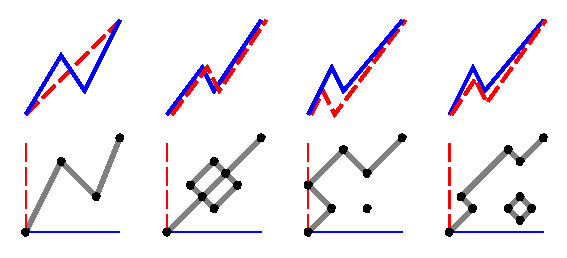
\includegraphics[scale=0.9]{Figs/Toughies/monks}
\end{figure} 
Ниже каждого варианта находится соответствующий график.
Заметим, что, как, например, в последнем случае, график может иметь участки, к которым у монахов нет доступа (без нарушения равенства высот).

Эту задачу мне показал Юлий Барышников из Лабораторий Белла.

\subsubsection*{Сумма под контролем}

Эта задача возникла «из реальной жизни», или, по крайней мере, из серьёзной задачи про волоконно-оптическую связь.\footnote{A. Schrijver, P. D. Seymour, P. Winkler, ``The Ring Loading Problem''. \emph{SIAM Review} Vol. 41, \#4 (Dec. 1999), 777--791.}
Гипотеза была обнародована, но не было найдено ни доказательств, ни контрпримеров.
Наконец автор этих строк нашёл доказательство приведённое ниже, которое ещё и оказалось довольно простым!

\medskip

Задача состоит в том, чтобы выбрать знаки в последовательности чисел из отрезка $[0,1]$ так, чтобы сумма оставалась под контролем даже при обращении знаков любого хвоста последовательности.
Первое наблюдение состоит в том, что можно управлять всеми \emph{начальными} суммами используя \emph{жадный алгоритм}, то есть ставить $y_k=x_k$, если $\sum_{i=1}^{k-1}y_i \le 0$ и $y_k=-x_k$ в противном случае.

Это гарантирует, что $\left|\sum_{i=1}^{k}y_i\right| \le 1$ для любого $k$ и, значит,
\begin{align*}
\left|\sum_{i=1}^{k}y_i-\sum_{i=k+1}^{n}y_i\right|&=\left|2\sum_{i=1}^{k}y_i-\sum_{i=1}^{n}y_i\right|\le
\\
&\le2\left|\sum_{i=1}^{k}y_i\right|-\left|\sum_{i=1}^{n}y_i\right|\le3.
\end{align*}

Это близко к тому, что нам надо. 
Однако оказывается, что любой алгоритм который не заглядывает вперёд, не может улучшить оценку с 3 до~2.
Чтобы это увидеть, представьте, что последовательность начинается как
1, 0,99, 1, 0,99, 1, 0,99, и так сто раз, но внезапно заканчивается некоторым числом $z$.
В этом случае знаки должны чередоваться каждый раз кроме одного момента, и чтобы узнать этот момент, необходимо знать $z$.

Однако заметим, что в описанном выше жадном алгоритме требуется знание «пустой суммы», чтобы выбрать первый знак.
Обычно мы считаем, что эта сумма равна 0, но давайте объявим её равной $w$.
Тогда, для фиксированного $w\in [-1,1]$ знаки $y_k$ определяются индуктивно как $y_k=x_k$, если $w+\sum_{i=1}^{k-1}y_i \le 0$, а иначе $y_k=-x_k$.
В этом случае $w+\sum_{i=1}^{k}y_i \in[-1,1]$ для любого $k$.
Рассмотрим функцию $f(w) \mathop{{:}{=}} w+\sum_{i=1}^ny_i$.

Предположим, что $f(w)=-w$.
Тогда
\begin{align*}
&\phantom{=}\sum_{i=1}^{k}y_i-\sum_{i=k+1}^{n}y_i=
\\
&=2\sum_{i=1}^{k}y_i-\sum_{i=1}^{n}y_i=
\\
&=2\left(w+\sum_{i=1}^{k}y_i\right)-\left(w+\sum_{i=1}^{n}y_i\right)-w=
\\
&=2\left(w+\sum_{i=1}^{k}y_i\right)\in[-2,2],
\end{align*}
что и требуется.

Поскольку  $f(-1)+(-1)<0 <f(1)+ 1$, существование $w$, для которого $f(w)=-w$ следовало бы из теоремы о промежуточном значении, если бы $f$ была непрерывна.
Конечно же, это не так; всякий раз, когда частичная сумма проходит через 0, некоторые знаки меняются, и $f(w)$ может совершить скачок.
(Заметим, что $f$ непрерывна слева, поскольку мы выбираем плюс при нулевой частичной сумме.)
Однако \emph{абсолютное значение} $f$ является непрерывным.

Сначала следует отметить, что, если частичные суммы не равны $0$, то производная $f'(w)$ равна 1.
С другой стороны, предположим, что $w=w_0$ таково, что хотя бы одна частичная сумма равна нулю.
Пусть $k>0$ --- минимальное значение, для которого $w+\sum_{i=1}^{k}y_i\z=0$.
Тогда для достаточно малых $\varepsilon>0$
знаки $y_j$ и $w+\sum_{i=1}^{j}y_i$ при $j>k$ меняются при переходе от $w=w_0$ к $w=w_0+\varepsilon$.
Взяв $j = m$, получаем, что $\lim_{w\to w_0^+}f(w)\z=-f(w_0)$.

То есть, если при $w=w_0$ любая из частичных сумм обнуляется, то $\lim_{w\to w_0^+}f(w)\z=-f(w_0)$, таким образом, функция $g$, определяемая как $g(w) =|f(w)|$, будет непрерывной и иметь производную $\pm1$ везде, кроме конечного числа точек.
Граф $g$ представляет собой зигзаг с производной $1$ при $g(w)=f(w)$ и $-1$ при $g(w)=-f(w)$.

Если определить функцию $h$, как $h (w) = -w$, то граф $h$ будет отрезком с угловым коэффициентом $-1$ и концами в $(-1,1)$ и $(1,-1)$;
этот отрезок обязан пересекать граф $g$.
Более того, он либо пересекает его в точке, где $g'(w) = 1$, либо совпадает с отрезком графа $g$ с угловым коэффициентом $-1$, в последнем случае самая левая точка отрезка также лежит и на графике $f$.
В обоих случаях мы получаем точку $w$, в которой $-w = g (w) = f (w)$. \heart

\subsubsection*{Двухлампoвая комната}

Эта головоломка является частью серьёзной задачи в распределённых вычислениях.%
\footnote{Больше об этом вопросе можно прочитать в статье M. J. Fischer, S. Moran, S. Rudich, and G. Taubenfeld, ``The Wakeup Problem''. \emph{Proc. 22nd Symp. on the Theory of Computing}, Baltimore, Maryland, May 1990.}
Решение, приведённое ниже, предложено Стивеном Рудичем из Университета Карнеги --- Меллона, известно как «протокол с качелями»\footnote{англ. \emph{see-saw protocol}.}.

\medskip

Для понимания этого протокола, удобно думать об одном из переключателей как о «переключателе с камушком»: в нём либо лежит камушек, либо он пуст; а о другом --- как о качелях, у доски качелей может быть опущен либо правый, либо  левый конец (противоположный конец доски должен быть при этом поднят).
Каждый заключённый начинает с двумя виртуальными камушками.

При первом посещении заключённый «садится на качели», при этом он поднимает опущенный конец доски качелей и
после этого навсегда остаётся на этой стороне доски (то есть он всегда помнит, на какую сторону он попал в первый раз), пока у него не закончатся камушки, в этот момент он опускает свой конец доски (это может произойти, только когда он наверху) и «слезает с качелей», то есть прекращает игру и далее не предпринимает никаких действий.

Пока заключённый на качелях,
при последующих посещениях он пытается избавиться от камушка каждый раз, когда его конец доски поднят,
и взять камушек, когда он опущен.
Чтобы отдать камушек, переключатель с камушком должен быть пустой;
в этом случае заключённый 
кладёт в него один свой камушек (формально говоря, он переключает переключатель с камушком и считает, что у него осталось на один камешек меньше).
Чтобы взять камушек, переключатель с камушком должен быть полным, в этом случае он берёт из него камушек.
Если же переключатель с камушком не находится в подходящем положении, то он не делает ничего.

Когда один из заключённых собирает $2n$ камушков, он объявляет, что все уже побывали в комнате.
Вывод очевиден, так как в начале было $2n$ или $2n+1$ камушков (в зависимости от начального положения переключателя с камушком), а камушки не уничтожаются и не создаются нашим протоколом, и, значит, каждый внёс свой вклад.

А почему мы должны достичь состояния, когда один игрок собрал все камушки?
Во-первых, следует отметить, что в \emph{любой} момент между посещениями либо 
(а) одинаковое число заключённых сидят на обоих концах доски, либо 
(б) заключённых, сидящих на поднятом конце, на один больше.
Действительно, если мы начинаем с состояния (а), то первый кто садится на качели переведёт его в состояние (б), если же кто-то слезет с качелей, то он опускает свою сторону, снова переводя в состояние (б).
Если же мы начинаем с состояния (б), то при посадке на качели число уравнивается, поскольку садятся на качели с опущенной стороны доски, и мы попадаем в состоянии (а).
Если же кто-то слезает, то он уменьшает число заключённых на поднятой стороне, снова переводя состояние в (а).

Теперь предположим, что все заключённые уже побывали в комнате, и что $k$ из них на качелях (остальные истратили свои камушки и слезли).
Из вышесказанного получаем, что пока $k>1$, на поднятой стороне доски будет, как минимум, один игрок и, как минимум, один --- на опущенной.
Тогда камушки будут перетекать от первых ко вторым, пока кто-то не истратит все свои камушки, уменьшая число заключённых, сидящих на качелях до $k-1$.
Когда $k$ пройдёт весь путь до $1$, у оставшегося игрока будут все $2n$ или $2n+1$ камушков, и процесс завершится, если это не случилось раньше.
\heart

Как до этого додуматься?
Не  знаю --- спросите у Рудича!

\subsubsection*{Площадь против диаметра}

Это, так называемое \emph{изодиаметрическое неравенство}, было получено Людвигом Бибербахом,\footnote{Bieberbach, L. ``Über eine Extremaleigenschaft des Kreises.'' \emph{Jahresbericht der Deutschen Mathematiker-Vereinigung}, 24 (1915), 247--250.}
Доказательство можно получить применив неравенство Бруна --- Минковского к фигуре и её симметричной копии.
Ниже приведённое решение дано также в книге «Математическая смесь» Джона Литлвуда, основанное на элементарных вычислениях.

\medskip

Диаметр замкнутой фигуры является наибольшим расстоянием между парой её точек.
Следует отметить, что не любая фигура диаметра 1 может быть помещена внутрь круга диаметра 1;
например, равносторонний треугольник со стороной 1 не таков.
Никто не знает площадь наименьшей области, в которую может поместиться каждая область диаметра 1; этот вопрос известен как \emph{задача Лебега}. 

Итак, как же показать, что круг имеет самую большую площадь из всех фигур диаметра 1, если такие фигуры не помещаются внутрь круга?
Пусть $\Omega$ есть замкнутая фигура на плоскости диаметра 1; попробуем вычислить площадь $\Omega$, используя полярные координаты.
Можно предположить, что $\Omega$ выпукла, так как переход к выпуклой оболочке не увеличивает диаметр.

Пусть $P$ и $Q$ являются точками $\Omega$ на расстоянии 1.
Поместим $\Omega$ в плоскости так, чтобы $P$ совпало с началом координат, а $Q$ с точкой $(1,0)$.
Пусть $R(\theta)$ --- точка, самая дальняя от $P$ под углом $\theta$ от оси $X$ против часовой стрелки, и пусть $r(\theta)$ --- расстояние от $P$ до $R(\theta)$.

\begin{wrapfigure}{r}{33mm}
\vskip-0mm
\centering
\includegraphics{Figs/mppic/pic-2}
\end{wrapfigure}

Тогда площадь $S$ фигуры $\Omega$ можно выразить как интеграл
\[S=\int\limits_{-\pi/2}^{\pi/2}\frac{r(\theta)^2}{2}d\theta.\]
Поскольку $r(\theta) \le 1$, он ограничен величиной
\[\int\limits_{-\pi/2}^{\pi/2}\frac{1}{2}d\theta=\frac\pi2.\]
Это вдвое больше, чем мы хотим, но не следует разочаровываться, поскольку до сих пор мы пользовались только тем, что $\Omega$ лежит в правой половине круга радиуса 1 с центром в начале координат.
Можно ещё подрезать полукруг до формы линзы, но как добиться оценки $\tfrac\pi4$?

Трюк заключается в разбиении интеграла на два в зависимости от знака $\theta$, и последующим преобразовании интеграла:
\begin{align*}
\int\limits_{-\pi/2}^{\pi/2}\frac{r(\theta)^2}{2}d\theta&=\int\limits_{-\pi/2}^{0}\frac{r(\theta)^2}{2}d\theta+\int\limits_{0}^{\pi/2}\frac{r(\theta)^2}{2}d\theta=
\\
&=\int\limits_{0}^{\pi/2}\frac{r(\theta-\tfrac\pi2)^2}{2}d\theta+\int\limits_{0}^{\pi/2}\frac{r(\theta)^2}{2}d\theta=
\\
&=\int\limits_{0}^{\pi/2}\frac{r(\theta-\tfrac\pi2)^2+r(\theta)^2}{2}d\theta.
\end{align*}
По теореме Пифагора, $r(\theta-\tfrac\pi2)^2+r(\theta)^2$ равно квадрату расстояния между $R(\theta)$ и $R(\theta- \pi/2)$.
Таким образом, это выражение ограничено квадратом диаметра $\Omega$ --- а именно, единицей.
В частности
\[S\le \int\limits_{0}^{\pi/2}\frac12d\theta\le\frac\pi4;\]
всё --- конец.
\heart

\subsubsection*{Разрез пополам}

Эта задача, с $n=100$, давалась на 4-й Всесоюзной математической олимпиаде в Симферополе, 1970.
Она достаточно красива, чтобы именоваться теоремой, и, на самом деле, так оно и есть.%
\footnote{P. Erd\H{o}s, A. Ginzburg, A. Ziv, ``Theorem in the Additive Number Theory''. \emph{Bull. Research Council of Israel}, Vol. 10F (1961), 41--43.}

\medskip

Назовём набор «ровным», если сумма его чисел сравнима с $0$ по модулю $n$.
Заметим сначала, что утверждение, которое мы хотим доказать, влечёт следующее, казалось бы, более слабое утверждение. 
Если набор $S$ из $2n$ чисел является ровным, то $S$ можно разбить на два ровных набора размера $n$ каждый.
Однако, из последнего утверждения вытекает, что любой набор размера $2n-1$ содержит ровный набор размера $n$.
Действительно, мы можем добавить к этому набору $2n$-е число, которое сделает исходный набор ровным, и затем применить предыдущее утверждение, чтобы разделить его на \emph{два} ровных набора размера $n$. 
Одно из них (то, что без нового числа) даёт решение.

Так что все три приведённые утверждения равносильны.
Предположим, что мы можем доказать второе для $n = a$ и для $n = b$.
Тогда, если набор $S$ имеет размер $2n = 2ab$ и сумму $0 \pmod {ab}$, то он, в частности, ровный по отношению к $a$. 
Значит, мы можем отсечь от него наборы $S_1,\dots,S_{2b}$, каждый размера $a$, которые также ровные по отношению к $a$.
Каждый из этих наборов $S_i$ имеет сумму, которую можно записать в виде $ab_i$.
Теперь числа $b_i$ составляют набор размера $2b$, сумма которого $0 \pmod b$, так что мы можем разбить $S$ на два набора размера $b$, которые являются ровными относительно $b$.
Объединение наборов $S_i$ в каждой части дают разбиение $S$ на два набора по $ab$ чисел в каждом, которые являются $ab$-ровными, как раз то, что и требовалось.

Отсюда следует, что если мы сможем доказать утверждение для всех простых чисел $n=p$, то мы докажем его для всех $n$.
Выберем набор $S$ размера $2p$ и начнём искать в нём $p$-ровный набор размера~$p$.

Как такой найти?
Один способ состоит в том, чтобы разбить числа в $S$ на пары и выбрать по одному числу из каждой пары.
Нам  надлежит позаботиться, чтобы числа в каждой паре давали различные остатки при делении на $p$, иначе в нашем выборе не будет разнообразия.

А можем ли мы это сделать? --- Да.
Упорядочим $S$ по модулю $p$ (скажем, от $0$ до $p-1$), и рассмотрим пары $(x_i,x_{i+p})$ при $i\z=1,2,\dots, p$.
Если $x_i\equiv x_{i+p}\pmod p$ для некоторого $i$, то $x_i,x_{i+1},\z\dots,x_{i+p}$ сравнимы по модулю $p$, и можно взять $p$ из них, чтобы составить желанный набор.

Теперь, когда у нас есть пары, применим «динамическое программирование».
Пусть $A_k$ есть множество всех сумм $\pmod p$, которые можно получить путём добавления по одному числу из первых $k$ пар.
Заметим, что $|A_1|= 2$.
Мы утверждаем, что $|A_{k+1}|\z\ge|A_k|$, и более того, $|A_{k+1}|>|A_k|$, если $|A_k|< p$.
Первое неравенство верно, так как $A_{k+1} = (A_k+x_{k+1}) \cup (A_k+x_{k+1+p})$.
Далее, если $|A_{k+1}|=|A_k|$, то эти два набора идентичны, и, значит,  $A_k \z= A_k+x_{k+1+p}-x_{k+1}$.
Но, поскольку $p$ простое и $x_{k+1+p}-x_{k+1}\not\equiv 0\pmod p$, это возможно только в двух случаях: $|A_k|= 0$ или $p$.

Поскольку всего пар $p$, получаем, что $|A_k|= p$ для некоторого $k \le p$ и, следовательно, $|A_p|= p$; в частности, $0\in A_p$ --- теорема доказана. \heart

\subsubsection*{Салфетки без метрдотеля}

Мы хотим вычислить вероятность того, что гость, сидящий в положении 0 (по модулю $n$), остался без салфетки.
Предел этой вероятности при $n\to\infty$ равен искомой доле бессалфеточников.

Можно предположить, что каждый решает заранее, брать салфетку справа или слева, в случае, если обе в наличии;
потом, конечно, некоторым придётся изменить своё решение или вовсе остаться без салфетки.

Предположим, что гости $1,2,\dots, i - 1$ решили брать салфетку справа  (в сторону от 0), а гость $i$ решил брать слева;
и также гости $-1,-2,\dots, -j + 1$ решили брать салфетку слева (опять же, в сторону от 0), в то время как гость $-j$ решил брать справа.

Если $k = i+j+1$, то вероятность такой конфигурации равна $2^{1-k}$.
Заметим, что $i$ и $j$, по меньшей мере, равны $1$, но, с большой вероятностью, каждое из них меньше $n/2$.

Гость $0$ остаётся без салфетки только тогда, когда он садится последним из гостей $-j,\dots,i$, и \emph{ни один} из гостей $-j\z+1,\z\dots,-1,1,\dots,i-1$ не смог взять салфетку, которую хотел.
Если $t(x)$ обозначает время, в которое гость $x$ хватает салфетку, то это происходит в точности тогда, когда $t(0)$ является единственным локальным максимумом $t(x)$ в диапазоне от $-j$ до $i$.
То есть график $t$ представляет собой «горку» с вершиной в $(0,t(0))$; 
а точнее, выполняются следующие неравенства: 
\[t(-j)\z<t(-j+1) \z<\z\dots\z<t(-1)\z<t(0)\z>t(1)\z>\z\dots\z>t(i).\]

Вместо подсчёта вероятности этого события при фиксированных $i$ и $j$ удобнее сгруппировать все пары $(i, j)$ с фиксированным $k=i\z+j+1$.
Всего существует $k!$ возможных порядков у $t(-j),\dots, t (i)$.
Пусть $T$ есть множество всех моментов хватания, а $t_{{\max}}$ --- последний из них. 
Заметим, что горка однозначно определяется подмножеством $\{t(1),\dots,t(i)\}$ в $T\backslash \{t_{{\max}}\}$.
Таким образом, число различных горок, равно $2^{k-1}-2$.

Суммируя вероятности по $k$, получим, что вероятность того, что гость 0 остался без салфетки, равна
\[\sum_{k=3}^\infty\frac{2^{1-k}\cdot(2^{k-1}-2)}{k!}=(2-\sqrt{e})^2\approx 0{,}12339675.\]
\heartf

Сравнивая это значение с дробью $9/64 = 0{,}140625$, достигнутой метрдотелем, мы видим, что его старания вредят, но не сильно.

\medskip

Тем читателям, что предпочитают интеграл сумме, понравится следующее доказательство (полученное упрощением подхода, предложенного Эйденом Садбери из Университета Монаша в Австралии).

\medskip

Можно предположить, что «времена хватания» $t(i)$ для всех гостей --- независимые случайные величины в отрезке $[0,1]$, заданные равномерным распределением.
Представим себе, что вместо круга гости садятся вдоль прямой, бесконечной в обе стороны.
Пусть $p(t)$ обозначает вероятность того, что у гостя, со временем хватания $t$ нет салфетки справа.
Это происходит только если его правый сосед схватил салфетку первым;
либо он выбрал её добровольно,
либо был вынужден взять левую салфетку, потому что его правая была уже взята.
Таким образом,
\[p(t)=\frac12t+\frac12\int\limits_0^tp(s)\,ds.\]
Продифференцируем это равенство по $t$ и решим полученное дифференциальное уравнение:
\begin{align*}
\frac{dp}{dt}&=\frac12+\frac12p,
\\
\frac2{p+1}dp&=dt,
\\
2\ln(p+1)&=t+C.
\end{align*}
Заметим, что $C=0$, поскольку $p(0)=0$.
Следовательно,
\[p(t) = e^{t/2} - 1.\]
Конечно же, вероятность того, что гость со временем хватания $t$ обнаруживает, что его \emph{левая} салфетка исчезла, такая же.
Сила подхода состоит в применении независимости этих двух событий.
Отсюда вероятность того, что наш гость станет бессалфеточником равна $p(t)^2 \z= (e^{t/2} -1)^2$, и усреднение по времени хватания даст
\[\int\limits_0^1(e^{t/2}-1)^2dt=(2-\sqrt{e})^2.\]
\heartf

\subsubsection*{Группа солдат в поле}

Назовём двух солдат «товарищами», если они присматривают друг за другом.
Как и в главе «Погружение», в любой группе, два ближайших друг к другу солдата являются товарищами.
Но в одной группе (скажем, размера $k$) не может быть другой пары товарищей, потому что тогда оставшихся $k-4$ присматриваний не хватило бы, чтобы связать вместе две пары товарищей и $k-4$ оставшихся солдат.
Таким образом, если известна вероятность $p$ того, что данный солдат имеет товарища, то мы знаем и средний размер группы $g$, поскольку $p = 2/g$ и, значит, $g = 2/p$.

\begin{figure}[h!]
\centering
\includegraphics{Figs/mppic/pic-1}
\end{figure}

Начнём с солдата $X$, стоящего посреди квадратного поля $F$ площадью в 1 квадратный километр.
Затем добавим $n$ солдат по одному за раз, каждый в случайном положении в пределах $F$. 
Мы считаем, что $n$ огромно.
Назовём второго солдата $Y$, будем использовать строчные буквы $x$ и $y$ для обозначения положений $X$ и $Y$.
Пусть $\text{Б}$ обозначит событие, когда $Y$ становится ближайшим солдатом к $X$, 
и $\text{Т}$ --- событие, когда $Y$ становится товарищем $X$.
Заметим, что $\mathbb{P}(\text{Б})=1/n$, поскольку $Y$ станет ближайшим к $X$ с той же вероятностью, что и любой другой солдат.
Остаётся найти $p=\mathbb{P}(\text{Т})/\mathbb{P}(\text{Б})$.

Чтобы произошло $\text{Б}$, требуется, чтобы другие солдаты не попали в круг с центром в $x$ и радиусом $r=|x-y|$.
Чтобы произошло $\text{Т}$, другие солдаты не должны попасть ни в этот круг, ни в перекрывающийся с ним круг того же радиуса с центром в $y$.
Отношение площадей первого и второго равно $c=\pi/(\tfrac43\pi+\tfrac{\sqrt{3}}{2}) \approx 0{,}6215049$.
(Конечно, это отношение не зависит от $r$; на рисунке дана подсказка, как вычислить $c$ при $r=1$.)

Пусть поле $F'$ содержит поле $F$ и имеет площадь $1/c$ квадратных километров.
Пусть $\text{Т}'$ обозначает событие, при котором остальные солдаты ставятся случайным образом в $F'$, а не в $F$, и $Y$ становится товарищем $X$.
Независимо от значения $r$, каждый новый солдат в $F'$ имеет ту же вероятность разрушить $\text{Т}'$, что и новый солдат в $F$ разрушить $\text{Б}$. 
Значит, $\mathbb{P}(\text{Т}')= \mathbb{P}(\text{Б}) = 1/n$.
Теперь предположим, что $Y$ сам выбрался из $F'$ вместо $F$.
Чтобы иметь шанс стать товарищем $X$, он должен быть в меньшем поле, что произойдёт с вероятностью $c$.
И как мы видели, если он оказался в $F$, то станет товарищем $X$ с вероятностью $1/n$.
Таким образом, $Y$ станет товарищем $X$ с вероятностью $c/n$, так что $p=c$.

Отсюда средний размер группы равен $2/p\approx3{,}2170956$.
\heart

Приведённое выше рассуждение не вполне строго, поскольку не учитывает краевых эффектов.
Любители интегрировать распределение Пуассона 
найдут более простым и, возможно, более убедительным, способ вычислить $p$, интегрируя по $r$:
\[p=\int\limits_0^\infty e^{-\pi r^2/c}\,2\pi r\, dr.\]
Однако приведённое выше рассуждение более общее и элементарное, и, за исключением вычисления $c$ оно не зависит от размерности.
Если солдаты находятся на прямой, то отношение $c$ равно $2/3$, и, значит, средний размер группы равен 3;
в пространстве (для боевых водолазов?) $c = 16/27$, давая средний размер группы $3\tfrac38$.
При увеличении размерности $c\to 1/2$ и $g\to 4$. 
Забавно, что ответы рациональны в измерениях 1 и 3, но не для плоскости.

Луис Годдин из Университета Саймона Фрейзера, показавший мне эту прелестную задачу и её решение, указал, что было бы не менее интересно найти вероятность того, что за каким-то солдатом никто не присматривает.
Ни он, ни я не знаем, как это сделать;
согласно экспериментам должно получиться около $28\%$ на плоскости (при $25\%$ на прямой).
Кстати сказать, граф, определённый на метрическом пространстве путём соединения каждой точки с её ближайшим соседом, иногда называется графом Габриэля.

\subsubsection*{Игреки на плоскости}

Следующее ловкое  доказательство, предложено Рэндоллом Доэрти из Университета штата Огайо.\footnote{Рассмотрена в R. L. Moore  ``Concerning triods in the plane and the junction points of plane continua''. \emph{Proc. Natl. Acad. Sci. USA} 14.1 (1928), 85--88.}

\medskip

Для каждого игрека (Y) построим тройку рациональных кругов (с рациональными центром и радиусом), содержащих конечные точки, и при этом достаточно малых --- таких чтобы ни один из них не пересекал и не содержал две другие руки игрека.

Мы утверждаем, что тройка игреков не может иметь одну и ту же тройку окружностей.
Если бы это было так, то можно было бы соединить середину каждого игрека с центром каждого круга, следуя по соответствующей руке до круга и далее по его радиусу в центр.
Это дало бы вложение полного двудольного графа $K_{3,3}$ в плоскость (этот граф известен по головоломке про домики и колодцы).

Другими словами, мы получили шесть точек на плоскости (тройка центров кругов и тройка середин игреков) таких, что каждая точка из одной тройки соединена кривой с каждой точкой другой тройки, и при этом никакие две кривые не пересекаются.
Это невозможно; читатели, знакомые с теоремой Понтрягина --- Куратовского знают этот граф как один из двух главных непланарных графов.

Чтобы самим убедиться в том, что $K_{3,3}$ не вкладывается в плоскость без самопересечений, рассмотрим два набора вершин $\{u, v, w\}$ и $\{x, y, z\}$.
Если бы мы смогли нарисовать его без самопересечений, то цикл $uxvywz$ представлял бы  собой (топологический) шестиугольник.
Ребро $uy$ должно пройти внутри или снаружи шестиугольника (скажем, внутри);
тогда $vz$ придётся пройти снаружи, чтобы избежать пересечения с $uy$, а ребру $wx$ уже пройти негде.
\heart

\subsubsection*{Снова  намагниченные доллары}

Этот вариант урн Пойа рассматривал Джоэл Спенсер из Нью-Йоркского университета и его студент Роберто Оливейра.
Очень чёткий способ показать, что одна из урн получит все монеты, за исключением конечного числа, состоит в использовании того самого процесса без памяти, который оказался полезным во второй задаче про гладиаторов из главы «Игры».

\medskip

Посмотрим только на первую урну.
Предположим, что среднее время ожидания между $n$-й и $(n+1)$-й монетой равно 
$1/n^{1{,}01}$ часам; при этом мы считаем, что этот процесс не имеет памяти.
Сначала монеты будут поступать эпизодически и неравномерно, а затем быстрее и быстрее.
Поскольку ряд $\sum 1/n^{1{,}01}$ сходится, урна взорвётся, то есть наполнится бесконечным числом монет в какой-то случайный момент (приблизительно через 4 дня).

Теперь представим, что два таких процесса идут одновременно, по одному с каждой урной.
Если в некоторый момент времени $x$ монет лежат в первой урне и $y$ --- во второй, то (как мы видели с гладиаторами-лампочками) 
вероятность того, что следующая монета попадёт в первую урну, составит
\[\frac{1/y^{1{,}01}}{1/x^{1{,}01}+1/y^{1{,}01}}=\frac{x^{1{,}01}}{x^{1{,}01}+y^{1{,}01}},\]
именно то, что и должно быть.
Поскольку процесс не имеет памяти,
не имеет значения, сколько времени прошло с тех пор, как $x$-я монета попала в первую урну (или $y$-я во вторую).
Из этого следует, что мы описали ускоренный вариант исходной задачи.

Однако теперь очевидно, что с вероятностью 1 моменты взрыва у двух урн различны.
(Для этого нужно только знать, что время ожидания взрыва имеет непрерывное распределение.)
Но эксперимент заканчивается при первом взрыве, в этот момент вторая урна остаётся с конечным числом монет.\heart

Выглядит пугающе, не так ли?
По сути, медленная урна не добралась до финиша, просто потому, что кончилось время.

\chapter*{Нерешённые головоломки}
\addcontentsline{toc}{chapter}{Нерешённые головоломки}

\setlength{\epigraphwidth}{.55\textwidth}
\epigraph{Человек не может учиться иначе, как двигаясь от известного к неизвестному.}{---Клод Бернар (1813---1878)}

Цитируя моего приятеля: «Нерешённая головоломка --- это что ещё за хрень такая?».
С этим можно согласиться, ведь невозможно узнать, имеет ли задача изящное решение, пока она не решена.
Тем не менее, некоторые нерешённые задачи привлекают красотой и простотой своей постановки, удивляя при этом тем, что решение неизвестно.
Математики, особенно такие, как и ваш автор, воспитанные в эрдёшовской традиции искать самое простое из непонятного, часто бравируют такими головоломками.
Соберите несколько таких фанатиков вместе, и вы услышите разговор вроде такого:

«Вот что меня беспокоит; ты знаешь ответ?»

«На самом деле, я даже не уверен, что знаю ответ на этот более простой вопрос.»

«Вы шутите? \emph{Я} даже не знаю \emph{вот этого}!»

Конечно, следует различать нерешённую головоломку и гипотезу, как, например, гипотезу Римана или P=NP.
Гипотезы могут не иметь красивой и элементарной формулировки, но они возникают на пути к истине (часто как препятствия) и поэтому их изучают.
Формулировка гипотезы часто требует «профессиональных» математических понятий (графы, группы, многообразия, преобразования, представления и тому подобное), которые не допускаются в головоломке, хотя они могут подразумеваться или быть необходимыми в её решении.

Нерешённые головоломки могут быть развлекательными, интригующими и даже пакостными,
но они не должны быть принципиально важны, \emph{по крайней мере, это не должно быть известно}.
Конечно, каждая нерешённая задача важна как пробел в нашем знании.
Её решение может натолкнуть на создание полезной техники;
или она может решиться приложением глубокой математики.
При этом некоторые задачи, приведённые ниже, такие, как гипотеза Франкла или $3x+1$ дилемма, привлекли столько внимания, что любое решение будет представлять значительный интерес, независимо от применимости его в других областях.

Эти задачи представлены здесь для развлечения и для того чтобы напомнить вам о том, как мало мы знаем.
Если даже одну из них кто-то решит, узнав про неё в этой книге, то случится небольшое чудо.
Если вам кажется, что вы решили одну из них, то скорее всего, вы ошибаетесь.
Воспользуйтесь приведенными ссылками, вашими профессиональными математическими друзьями и вашей любимой поисковой системой в интернете, чтобы узнать больше о других попытках решить эту задачу.
Скорее всего вы узнаете, что попали в известную ловушку, и не опозоритесь на публике.

Если же вы все еще считаете, что у вас есть настоящее решение, то оно должно быть записано и отправлено в подходящий математический журнал.
Не отправляйте его ко мне: я не являюсь экспертом ни в одной из этих задач.

\medskip

В этой главе, конечно, не будет раздела решений, но мы продолжим формат: формулировки сначала, а комментарии и ссылки потом.
Начнем с классики от Джона Конвея.
Удачи!


\subsection*{Ангел и Дьявол Конвея}
\rindex{Ангел и Дьявол Конвея}

Ангел летает над бесконечной шахматной доской, и время от времени должен садиться на клетку.
Он может пролететь не более 1000 ходов короля до очередного приземления.

Пока Ангел летит, Дьявол, живущий под доской, может уничтожить одну клетку по своему выбору.

Может ли Дьявол поймать Ангела?

\subsection*{$\bm{3x+1}$ дилемма}
\rindex{$3x+1$ дилемма}

Начиная с произвольного положительного целого числа, будем повторять следующее действие: если оно чётно, то сократим его вдвое, а если нечётно, утроим его и добавим 1.

Доказать, что в конце концов мы зациклимся; или даже сильнее, что в конечном итоге придём к циклу $1, 4, 2, 1, 4, 2,\dots$.

\subsection*{Самая длинная общая подпоследовательность}
\rindex{Самая длинная общая подпоследовательность}

Генерируются две случайные двоичные последовательности длиной $n$, причём каждая цифра определяется независимо и равна 1 с вероятностью $p$.
Пусть $C_p(n)$ есть средняя длина самой длинной общей подпоследовательности в обоих, и пусть $C_p$ есть предел отношения $C_p(n)/n$.

Вычислите $C_{\frac12}$ или, по крайней мере, докажите, что $C_{\frac12}<C_{p}$ при $p\ne\tfrac12$.

\subsection*{Квадратура озера}
\rindex{Квадратура озера}

Докажите, что каждая простая замкнутая кривая на плоскости содержит четвёрку точек в вершинах квадрата.

\subsection*{Одинокий бегун}
\rindex{Одинокий бегун}

Бегуны  стартуют в одной точке и бегут по круговой дорожке единичной длины;
каждый бежит с постоянной скоростью и скорости у всех различны.

Доказать, что каждый бегун в какой-то момент времени будет на расстоянии хотя бы $1/n$ от любого другого бегуна.

\subsection*{Сортировка шаров}
\rindex{Сортировка шаров}

В ряд стоит $n$ корзинок с парой шаров в каждой, при чём в $i$-той корзинке лежат шары с номерами $n+1-i$.
За одну операцию разрешается поменять два шара в соседних корзинках.

Сколько операций необходимо для того, чтобы каждый шар попал в корзинку со своим номером?

\begin{figure}[h!]
\centering
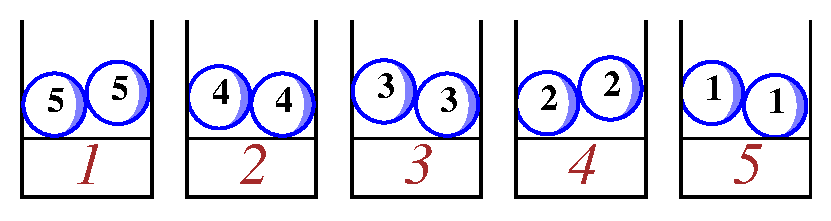
\includegraphics[scale=0.5]{Figs/UnsolvedPuzzles/bins}
\end{figure}

\subsection*{Развёртка многогранника}
\rindex{Развёртка многогранника}

Доказать, что произвольный выпуклый многогранник можно разрезать по рёбрам, так что полученную поверхность можно развернуть в плоский многоугольник.

\subsection*{Освещение многоугольника}
\rindex{Освещение многоугольника}

Любой ли многоугольник с зеркальными сторонами можно осветить одной лампочкой горящей в некоторой его внутренней точке?

\subsection*{Треклы Конвея}
\rindex{Треклы Конвея}

Треклом называют диаграмму на плоскости, состоящей из вершин и рёбер (кривых без самопересечений), такую что:
\begin{itemize}
\item каждое ребро начинается и заканчивается в двух различных вершинах, и не проходит через другие вершины; и
\item любая пара рёбер пересекает друг друга ровно один раз, либо в общей вершине, либо во внутренней точке.
\end{itemize}

Существует ли трекл с б\'{о}льшим числом рёбер, чем вершин?

\begin{figure}[h!]
\centering
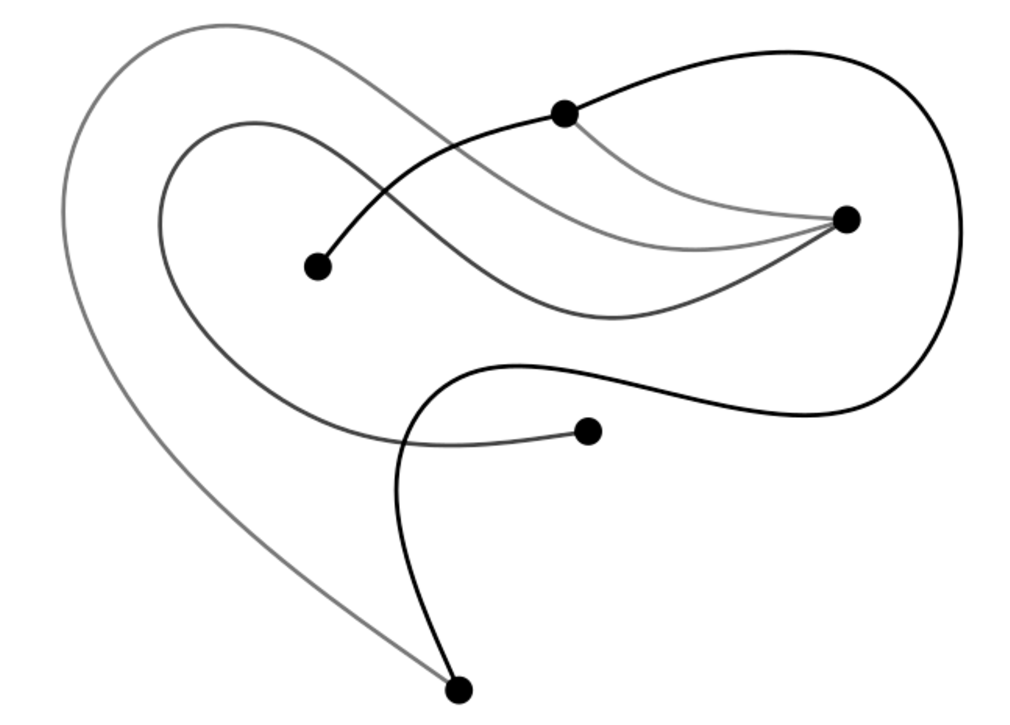
\includegraphics[scale=0.5]{Figs/UnsolvedPuzzles/thrack}
\end{figure}

\subsection*{Затор}
\rindex{Затор}

Вершины бесконечной решётки на плоскости выбираются независимо с фиксированной вероятностью $p\in (0,1)$.
В каждую из выбранных вершин помещают автомобиль направленный либо на север либо на восток,
в каждом  случае направление выбирается независимо подкидыванием монетки.

Движение регулируется светофорами, которые включают поочерёдно «зеленый-восточный» и «зеленый-северный».
При включённом зеленом-восточном, каждый восточный автомобиль, правая соседняя вершина от которого не занята, перемещается в эту вершину; остальные (в том числе заблокированные другим восточным автомобилем) остаются там, где они находились.

Когда включается зеленый-северный, каждый незаблокированный автомобиль в северном направлении перемещается на одну вершину в северном направлении.

Эксперименты говорят, что если $p$ ниже определённого критического значения $p_0$,
то автомобили постепенно разъезжаются.
Более того каждый автомобиль имеет предельную среднюю скорость, равную скорости автомобиля, который никогда не блокируется.
Но когда $p> p_0$ происходит обратное: автомобили попадают в безнадёжный затор, то есть каждый автомобиль делает только конечное число переездов, и останавливается навсегда.

Если вы готовы в это поверить, то попробуйте доказать одно из этих утверждений.

\subsection*{Средние уровни}
\rindex{Средние уровни}

Докажите, что все подмножества размера $n$ или $n+1$ в множестве размера $2n+1$, можно обойти циклически добавляя или удаляя по одному элементу за раз.

\subsection*{Построение диаграмм Венна}
\rindex{Построение диаграмм Венна}

Диаграмма Венна порядка $n$ представляет собой набор из $n$ простых замкнутых кривых на плоскости, с трансверсальнымии пересечениями  по две кривые в точке и при этом для любого поднабора кривых, множество точек внутри кривых из поднабора, и снаружи остальных кривых является непустым и связным.

Любую ли диаграмму Венна порядка $n$ можно ли расширить до диаграммы Венна порядка $n+1$?

\subsection*{Стратегия для игры в щёлк}
\rindex{Стратегия для игры в щёлк}

Алиса и Боб играют в следующую игру:
Фиксируется число $k$.
Алиса называет делитель $k$.
Боб называет другой делитель $k$, который не кратен последнему числу названным Алисой.
Алиса называет третий делитель, который не является кратным ни одному из уже назаванных; 
и так далее.
Проигравает тот, кто называет 1.

Обратите внимание, что при $k=2^{n}\cdot 3^{m}$, эта игра эквивалентна игре щёлк из предыдущей главы для плитки шоколада $(m+1)\z\times (n+1)$.
То же рассуждение показывает, что у Алисы существует выигрышная стратегия, но остаётся следующая задача, как для версии с шоколадкой, так и для приведённого обобщения:

Найдите выигрышную стратегию для Алисы!

\subsection*{Все дороги ведут в Рим}
\rindex{Все дороги ведут в Рим}

Дана сеть (не обязательно плоская) из городов и односторонних дорог со следующими свойствами:
из каждого города выходят ровно две дороги, и для некоторого фиксированного $n$, можно добраться из любого города в любой другой город пройдя по $n$ дорогам.

Докажите, что можно раскрасить дороги в красный и синий цвет таким образом, что (а) каждый город имеет выездную дорогу каждого цвета, и (б) есть набор инструкций (например, КССКК), который всегда заканчивается в одном и том же городе, независимо от исходного города.

\subsection*{Круги в круге}
\rindex{Круги в круге}

Докажите, что любой набор кругов с общей площадью $1$ можно упаковать в круг площади $2$.

А ещё лучше было бы доказать, что в $d$-мерном пространстве любой набор из подобных копий выпуклого тела, с общим объёмом~1, можно упаковать в подобную копию объёма $2^{d-1}$.

\subsection*{Гипотеза Франкла}
\rindex{Гипотеза Франкла}

Пусть $U$ --- конечное множество, а $T$ --- семейство непустых подмножеств в $U$, замкнутое относительно объединения.
Докажите, что в $U$ есть элемент, принадлежащий, по меньшей мере, половине множеств в $T$.

\section*{Комментарии и ссылки}

\subsubsection*{Ангел и Дьявол Конвея}

Недавний обзор этой увлекательной головоломки содержится в очень симпатичной коллекции под редакцией Ричарда Новаковского.\footnote{\emph{Games of No Chance.} Edited by Richard Nowakowski, Cambridge University Press, Cambridge, 1996. \href{http://library.msri.org/books/Book29/}{\url{library.msri.org/books/Book29/}}.} 

Элвин Берлекэмп,  показал, что если Ангел обладает «силой 1», то есть может делать только одиночные ходы короля, то Дьявол побеждает.
Может оказаться, что Дьявол побеждает независимо от силы Ангела; 
однако, похоже на то, что силы 2 достаточно для того, чтобы Ангел выжил.

Ангел силы 1000 должен быть в состоянии выжить, но как сам изобретатель головоломки говорит в своей статье, на путях к решению возникают помехи.
Одна из них заключается в том, что Дьявол не может ошибиться;
то есть независимо от того, какую клетку он уничтожит, полученная конфигурация станет для него лучше чем начальная.
Другая заключается в том, что Дьявол, кажется, имеет ответ на любую простую стратегию «потенциальной функции», которой мог бы воспользоваться Ангел;
то есть, стратегия, которая говорит ему, куда ходить в зависимости от того, какие клетки уничтожены. 

Кроме того, если Ангел имеет какие-то, казалось бы, лёгкие недостатки вроде того, что ему запрещено ступать на клетку в далее чем на $10^{99}$ клеток к югу от клетки на которой он уже побывал, то Дьявол побеждает.

Сам Конвей похоже верит в Ангела, об этом свидетельствует то, что он предлагает приз в тысячу долларов за доказательство того, что Дьявол побеждает, и только сто за стратегию для достаточно сильного Ангела.

[Со времени публикации английского оригинала этой книжки, задача была независимо решена как минимум 4 раза.
Решения Оддвара Клостера%
\footnote{
O. Kloster, 
``A solution to the angel problem''.
\emph{Theoret. Comput. Sci.} 389 (2007), no. 1-2, 152--161.}
и Андре Мате%
\footnote{
A. Máthé, 
``The angel of power 2 wins''. 
\emph{Combin. Probab. Comput.} 16 (2007), no. 3, 363–374.}
работают для ангела силы 2.
Решение Брайна Боудича%
\footnote{B. H. Bowditch, ``The angel game in the plane''. \emph{Combin. Probab. Comput.} 16 (2007), no. 3, 345--362.}
работает для ангела силы 4.
Решения Питера Гакса%
\footnote{G. Peter, \emph{The angel wins.} \href{https://www.cs.bu.edu/~gacs/papers/angel.pdf}{\url{www.cs.bu.edu/~gacs/}}.}
работает для ангела много большей силы.]

\subsubsection*{$\bm{3x+1}$ дилемма}

Эта головоломка известна также как гипотеза Коллатца, сиракузская задача, задача Какутани, алгоритм Хасса и гипотеза Улама.
Мало что известно об её источнике, известно, что 1 июля 1932 года, студент Гамбургского университета по имени Лотар Коллатц записал похожую задачу в свою тетрадь, но задача известная теперь, кажется, стала популярна только в 1950-е годы.

Джефф Лагариас из лабораторий AT\&T написал о ней очень хороший обзор.\footnote{J. Lagarias, ``The 3x+1 Problem and its Generalizations''. \emph{Amer. Math. Monthly}, Vol. 92 (1985), 3--23,%\href{http://www.cecm.sfu.ca/organics/papers/lagarias/}{\url{www.cecm.sfu.ca/organics/papers/lagarias/}}.
}

Лагариас указывает на то, что эта головоломка, упоминалась как часть заговора с целью замедлить математические исследования в США.
Пусть это послужит предупреждением!

\subsubsection*{Самая длинная общая подпоследовательность}

Эта задача известна как минимум с 30-х годов; она упоминается в диссертации В. Данчика 1974 года защищённой в Уорикском университете.
Майкл Стил (Пенсильванский университет) сформулировал гипотезу, что $C_{1/2} = 2/(1+\sqrt{2})\approx 0{,}828427$.
Вацлав Хватал и Давид Санкофф показали, что $0{,}773911 < C_{1/2} < 0{,}837623$, и это дало основание предполагать, что число Стила великовато;
в конце концов, Джордж Люкер (Калифорнийский университет в Ирвайне) прикончил гипотезу, доказав, что $0{,}7880 \z< C_{1/2} \z< 0{,}8263$.\footnote{
G. Lueker, 
``Improved bounds on the average length of longest common subsequences''. \emph{Proceedings of the Fourteenth Annual ACM-SIAM Symposium on Discrete Algorithms} (Baltimore, MD, 2003), 130–131.}

Существование $C_p$ легко следует из субаддитивности,\footnote{см., например, R. Durrett, \textit{Probability: Theory and Examples,} Wadsworth, 1991, Section 6.6.} но это не позволяет вычислить саму константу.
Вот ещё подобный пример: Бела Боллобаш и я доказали существование числа $K_d$ такого, что самая длинная координатно-возрастающая цепь среди $n$ случайных точек в $d$-пространстве имеет средний размер равный $K_d\cdot n^{1/d}$.
Мы знаем, что $K_1=1$, $K_2=2$ и $\lim_{d\to\infty} K_d=e$, но не знаем чему равно $K_3$.

Если менять вероятность $p$, то конечно же $C_p>p$ при $p \z> 1/2$, так как можно смотреть только на подпоследовательности, состоящие из одних единиц.
Таким образом, $C_p\to 1$ при $p\to 1$, и это даёт основание предполагать, что $C_p$ минимально при $p=1/2$.
Чтобы это доказать, не обязательно знать точные значения $C_p$,
но, как это сделать, пока никто не знает.

\subsubsection*{Квадратура озера}

Хорошее обсуждение этой головоломки дано на «Геометрической свалке» Давида Эпштейна.%
\footnote{\href{http://www.ics.uci.edu/~eppstein/junkyard/jordan-square.html}{\url{www.ics.uci.edu/~eppstein/junkyard/jordan-square.html}}}
Похоже, что есть доказательства того, что квадрат можно вписать во все достаточно гладкие замкнутые плоские кривые.%
\footnote{Например W. Stromquist, ``Inscribed Squares and Square-Like Quadrilaterals in Closed Curves''. \emph{Mathematika}, Vol. 36 (1989), No. 2, 187--197.}
Тем не менее, в общем случае гипотеза остаётся открытой уже более 90 лет.%
\footnote{V. Klee, S, Wagon, \emph{Old and New Unsolved Problems in Plane Geometry and Number Theory.} MAA, 1991.}

\medskip

Как-то неловко признать, что математики не способны вписать квадрат в любую замкнутую плоскую кривую.

\subsubsection*{Одинокий бегун}

{

\sloppy

Эта замечательная гипотеза, была по-видимому, выдвинута Йоргом Виллсом.%
\footnote{J. M. Wills, ``Zwei Satze uber Inhornogene Diophantische Approximation von Irrationalzahlen''. \emph{Monatsch. Math.}, Vol. 71 (1967), 263--269.}
В 1973 году её независимо сформулировал Томас Кьюсик.
В 1984 году он вместе с Карлом Померансом доказал гипотезу для не более, чем пяти бегунов.
Том Бохман, Рон Хольцман и Дэн Клейтман (те самые, что из ящиков и подъящиков) доказали её для шести,%
\footnote{T. Bohman, R. Holzman, D. Kleitman,
``Six lonely runners''.
\emph{Electron. J. Combin.} 8 (2001), no. 2.
%\href{https://www.combinatorics.org/ojs/index.php/eljc/article/view/v8i2r3/pdf}{\url{www.combinatorics.org/ojs/index.php/eljc/article/view/v8i2r3/pdf}}
}
есть также более короткое доказательство Джерома Рено.%
\footnote{J. Renault, ``View-obstruction: a shorter proof for 6 lonely runners''. \emph{Discrete Math.} 287 (2004), no. 1-3, 93--101.}

}

\medskip

Название головоломке предложил Луис Годин из Университета Саймона Фрейзера.

Головоломка носит численно-теоретический характер;
можно доказать, что достаточно рассмотреть только случай целых скоростей.

\subsubsection*{Сортировка шаров}

Эта любопытная задачка возникла в Bellcore (ныне iconectiv) при статистических исследованиях предпочтений заказов.
Я работал над ней с коллегами Майклом Литтманом (ныне в Рутгерсе) и Грэмом Бригиттом (Лондонская школа экономики).
Задача обобщается не только на $k$-шарные корзинки, но и на корзинки с различным числом шаров.
Мы сосредоточимся только на двухшарном случае.

\medskip

Если бы корзинки были одношарные, то задача превратилась бы в простое упражнение.
В этом случае  для сортировки требуется $\binom{n}{2}$ перекладываний.
Один из способов это увидеть --- смотреть за числом пар шаров находящихся в обратном порядке, заметив, что одно перекладывание исправляет только одну пару.
Это рассуждение также говорит, что если не делать глупостей (а именно, не менять шары, которые уже находились в правильном порядке), то потребуется ровно $\binom{n}{2}$ перекладываний.
Более того, независимо от начальной конфигурации, $\binom{n}{2}$ перекладываний достаточно --- как и следовало ожидать, обратный порядок является наихудшим.

\medskip

Похоже, что те же рассуждения работают и с двухшарными корзинками.
Можно думать, что у нас по $n$ шаров двух цветов, красных и зелёных, и шары каждого цвета пронумерованы от $1$ до~$n$.
Если сортировать каждый цвет по отдельности, то закончим за $2\binom{n}{2}$ перекладываний.
Наверняка $2\binom{n}{2}$ шагов необходимо, верно?

А вот и нет!
В случае $n = 5$ (посмотрите на приведённую ниже диаграмму)
\begin{figure}[h!]
\centering
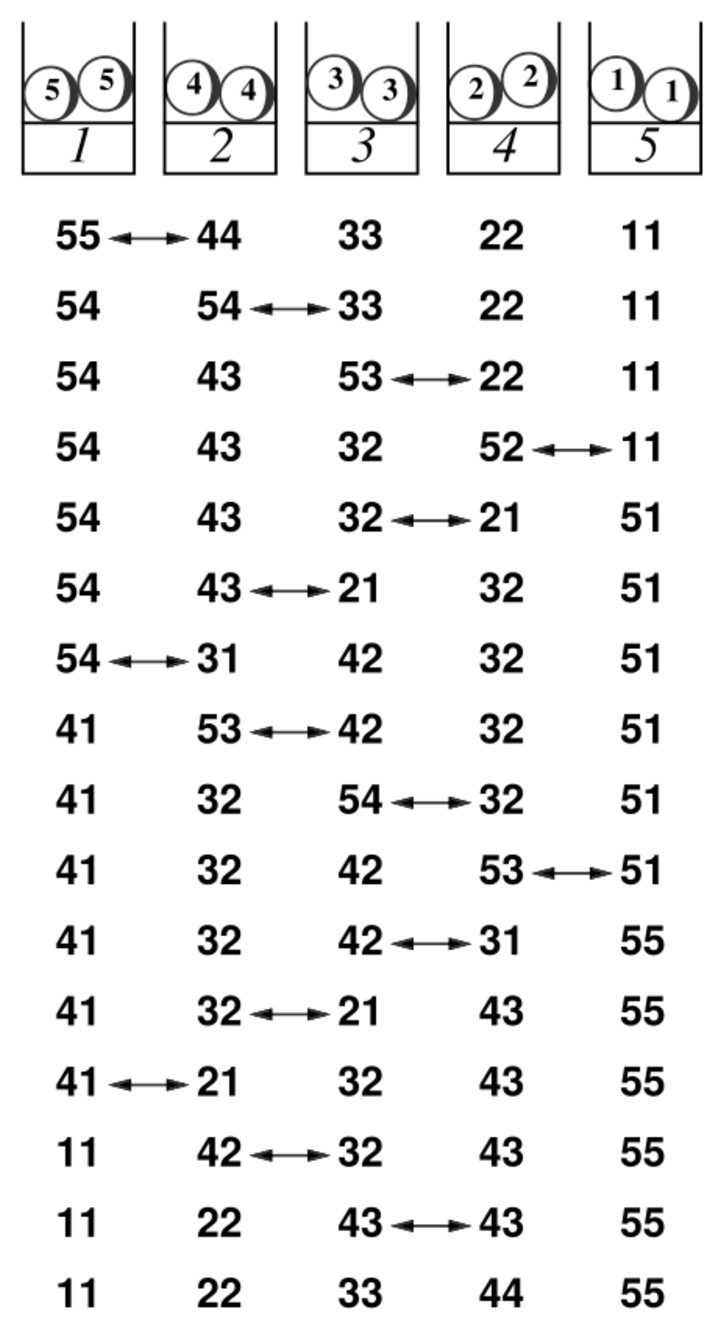
\includegraphics[scale=0.5]{Figs/UnsolvedPuzzles/5bin}
\end{figure}
волшебным образом шары упорядочились за 15 переклдываний, вместо 20, которые казались необходимыми.

Меньше чем за 15 перекладываний этого добиться нельзя; более того $\lceil\binom{2n}{2}/3\rceil$ перекладываний необходимо для упорядочивания шаров в $n$ двухшаных корзинках.
Чтобы увидеть это, присудим одно очко за обгон, то есть за то, что шар с б\'{о}льшим номером, прошёл слева направо относительно шара с меньшим номером.
Если обгон проделывается в два приёма, то мы назначаем по пол очка за то, что шар «поравнялся» и за то, что «ушёл вперёд».
Кроме того заметим, что в процессе любая пара шаров с одинаковыми номерами должна разделиться, а потом сойтись вместе --- накинем ещё по пол очка за каждое такое перекладывание. 
Всего получится $\binom{2n}2$ очков, которые придётся собрать в процессе сортировки.

А сколько очков можно заработать за одно перекладывание?
Предположим, что мы поменяли шары с номерами $u$ и $y$ из корзинки, с $u$ и $v$, и другой корзинки с $x$ и $y$.
Мы можем получить одно очко за то, что $u$ обогнал $y$,
по пол очка за то, что $u$ ушёл вперёд от $v$
и за то, что $x$ ушёл вперёд от $y$,
а ещё по пол очка за то, что $u$ поровнялся с $x$ 
и за то, что $v$ поровнялся с $y$.
Получается максимум 3 очка за перекладывание;
отсюда следует обещанная оценка.


Есть ещё хорошие новости.
Как и в случае одношарными корзинками, нетрудно показать, что самый плохой случай это обратный порядок.
То есть, если $f_2(n)$ обозначает минимальное число перекладываний, необходимых для сортировки шаров в $n$ двухшарных корзинках из любой начальной конфигурации, то ровно $f_2(n)$ перекладываний потребуется для сортирвки обратного порядка.
Также легко доказать, что если обмен должен быть сделан между $i$-той и $(i+1)$-ой корзинками, то не может быть неправильным перекладывать шар с наибольшим номером в $i$-той корзинке с шаром с наименьшим номером в $(i+1)$-ой корзинке.

Но есть и плохие новости, иначе задача не появилась бы в этом разделе.
Оценка $\lceil\binom{2n}{2}/3\rceil$ не всегда достижима.
Например, она даёт $f_2(6)\ge 21$, но на самом деле перебор проделанный на компьютере не нашёл способа провести сортировку шаров в шести двухшарных корзинках менее чем за 22 шага.
Хуже того, закономерность перекладываний для пяти корзинок показанная на диаграмме, обычно не оптимальна для большего числа корзинок.

Но всё ещё возможно, что какая-то другая закономерность оптимальна, и, возможно, она даёт формулу для $f_2(n)$.

\subsubsection*{Развёртка многогранника}

Есть основания полагать, что эта головоломка \emph{очень} старая. 
Во всяком случае развёртки многогранников рассматривались уже в книге с длинным заглавием «Руководство к измерению циркулем и линейкой, в плоскостях и целых телах, составленное Альбрехтом Дюрером и напечатанное с соответствующими чертежами в 1525 году на пользу всем любящим искусство».
Если надо разукрасить многогранник, то полезно разрезать его вдоль рёбер развернуть на плоскости без перекрытий.

По-видимому первая точная формулировка этой головоломки дана Г. С. Шепардом из Университета Восточной Англии.%
\footnote{G. C. Shephard, ``Convex Polytopes with Convex Nets''. \emph{Math. Proc. Camb. Phil Soc}, Vol. 78 (1975), 389--403.}
 
Известно, что существуют \emph{не}выпуклые неразвёртываемые многогранники%
\footnote{M. Bern, E. Demaine, D. Eppstein, E. Kuo, A. Mantler, J. Snoeyink, 
``Ununfoldable polyhedra with convex faces''.
\emph{Comput. Geom.} 24 (2003), no. 2, 51-–62.};
также существуют выпуклые многогранники, у которых наряду с честными развёртками есть развёртки с самоперекрытиями. 
Пара развёрток тетраэдра, с перекрытием и без, построенная Макото Намики из Токийского университета, показана ниже.

\begin{figure}[h!]
\centering
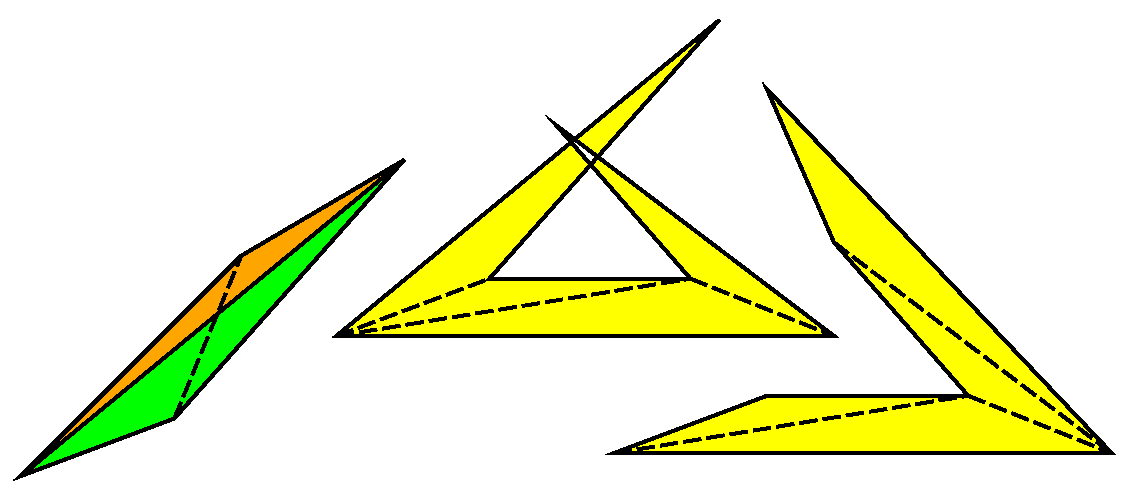
\includegraphics[scale=0.5]{Figs/UnsolvedPuzzles/unfold}
\end{figure}

Между прочим, может это покажется интересным --- не по каждой развёртке можно восстановить исходный выпуклый многогранник однозначно. %реф

Обсуждение этой задачи и дополнительные картинки можно найти на домашней странице Комеи Фукуда из Высшей технической школы Цюриха.%
\footnote{\href{https://inf.ethz.ch/personal/fukudak/old/}{\url{inf.ethz.ch/personal/fukudak/old}}}

\subsubsection*{Освещение многоугольника}

В своей книге,%
\footnote{J. O'Rourke \emph{Art Gallery Theorems and Algorithms.} Oxford University Press, 1987.}
Джозеф О’Рурк % (Joseph O' Rourke) 
из Смит Колледжа, утверждает, что источник этой головоломки неизвестен.
Виктор Кли написал о ней в 1969 году, в статье вышедшей в «American Mathe\-ma\-tical Monthly», которая привлекла большое внимание. 

Если считать, что луч попавший в вершину поглощается, то можно построить многоугольник, который не освещён из некоторой своей внутренней точки.
Пример, представленный ниже, найден Джоржем Токарским в 1995 году.

\begin{figure}[h!]
\centering
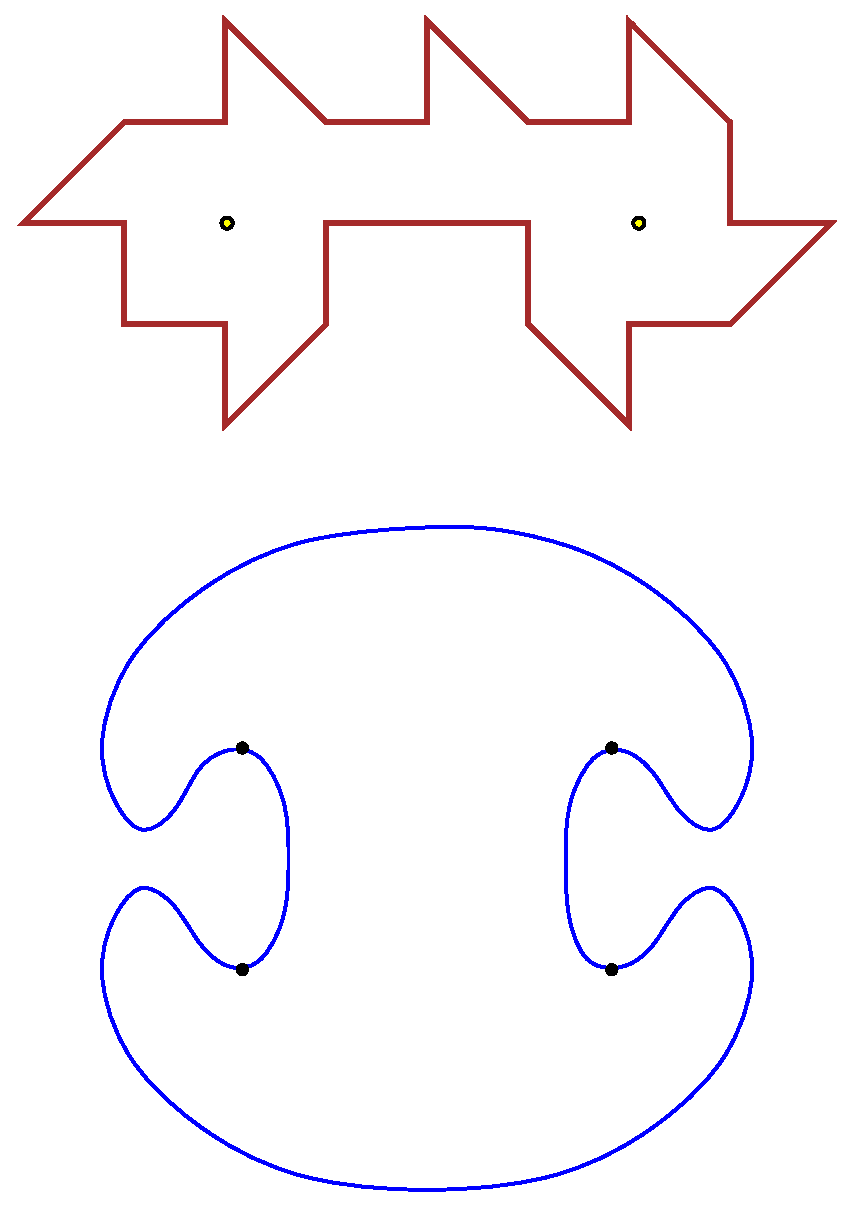
\includegraphics[scale=0.5]{Figs/UnsolvedPuzzles/vision}
\end{figure} 

О’Рурк полагает, что в любом зеркальном многоугольнике $P$ множество внутренних точек, из которых $P$ не может быть освещено, имеет меру 0.
Более того, если вершины заменяются небольшими круглыми дугами, то таких точек вовсе нет.

{\sloppy

Можно сконструировать фигуру ограниченную гладкой замкнутой кривой, которая не может быть освещена ни из одной своей внутренней точки. 
Такой пример был построен самим сам Кли (показан здесь), он использует два полуэллипса с фокусами в указанных точках.%
\footnote{Практически идентичный пример приведён ранее в заметке L. Penrose, R. Penrose, ``Puzzles for christmas''. \emph{New Scientist} 25 (1958), 1580--1581.}
Источник света в верхней половине, оставляет тёмной левую и правую доли на нижней половине.

}

\begin{figure}[h!]
\centering

\includegraphics[scale=0.5]{Figs/UnsolvedPuzzles/klee}
\end{figure} 

Есть довольно много других интригующих вопросов про зеркала.
Например, может ли конечный набор разделённых сегментных зеркал захватывать свет от источника?
А что насчёт зеркал в форме дуг окружностей?
Это и многое другое можно найти на слайдах замечательного доклада О’Рурка.%
\footnote{J. O'Rourke, ``Unsolved Problems in Visibility,''
\href{http://archive.dimacs.rutgers.edu/dci/2001/Visibility.ppt}{\url{archive.dimacs.rutgers.edu/dci/2001/Visibility.ppt}}.}

\subsubsection*{Треклы Конвея}

Эта интригующая гипотеза Конвея относится к 60-м годам.%
\footnote{D. R. Woodall, ``Thrackles and Deadlock''. \emph{Combinatorial Mathematics and its Applications}, Proceedings of a Conference held at the Mathematical Institute, Oxford (1969), 335--348.}
Её можно свести к тому, что два чётных цикла, склеенных по вершине невозможно представить как трекл;
что конечно ещё более возмутительно.
Лучшая оценка даёт, что число рёбер не может превышать удвоенное число вершин минус~3.%
\footnote{L. Lovasz, J. Pach, M. Szegedy, ``On Conway's Thrackle Conjecture''. \emph{Discrete and Computational Geometry}, Vol. 18 (1997), 369--376.}

У этой головоломки имеется свой фан-клуб.%
\footnote{\href{http://www.thrackle.org}{\url{www.thrackle.org}}.}

\subsubsection*{Затор}

Эта модель возникала при изучении транспортного потока на пересечении двух широких улиц.%
\footnote{O. Biham, A. A. Middleton, D. Levine, ``Self Organization and a Dynamical Transition in Traffic Flow Models''. \emph{Phys. Rev. A}, Vol. 46.10 (1992) R6124.}
Её странное поведение вызвало большой интерес.%
\footnote{Библиографию можно найти по адресу \href{http://cui.unige.ch/spc/Bibliography/traffic.html.}{\url{cui.unige.ch/spc/Bibliography/traffic.html}}.}
Ниже показаны фрагменты конфигураций, свободной и блокированной, каждая из которых в некоторой степени типична в экспериментах, поведённых Раисой Де Соуза из Microsoft Research.

\begin{figure}[h!]
\centering
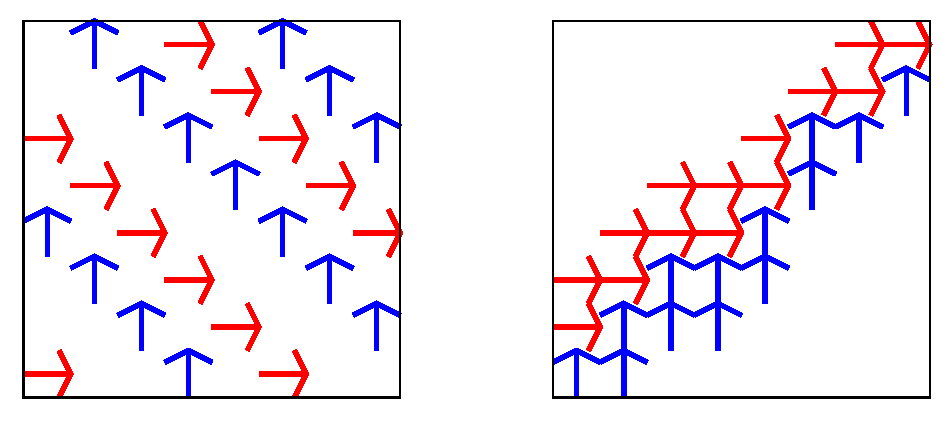
\includegraphics[scale=0.5]{Figs/UnsolvedPuzzles/gridlock}
\end{figure}

Если бы только доказать, что для некоторых $p$, пусть даже очень близких $0$ или $1$, поведение на самом деле такое...

[Со времени публикации английского оригинала этой книжки, случай $p\approx 1$ был решён Омером Энджелом,
Александром Холройдом и Джеймсом Мартином.
\footnote{O. Angel, A. Holroyd, J. Martin, 
``The jammed phase of the Biham--Middleton--Levine traffic model''.
\emph{Electron. Comm. Probab.} 10 (2005), 167--178.}]

\subsubsection*{Средние уровни}

Эта знаменитая головоломка о гамильтоновом цикле приписывалась комбинаторикам Ивану Гавелю, Клоду Берже, Итало Деджтеру, Палу Эрдёшу, У. Т. Троттеру и Дэвиду Келли.
Вероятно Гавел был первым.
Конечно, вопрос достаточно естественный, чтобы переоткрываться вновь и вновь.
Келли представил головоломку на конференции в Обервольфахе в 1981 году и получил приз (бутылку вина) за самую короткую гипотезу.

%Предупреждение читателю: Эта задачка заразительна. %и действительно, эксперименты привели многих интеллектуальных следователей к мнению, что существует модель, которая будет работать для любого $n$.
%Никто не верит, что предположение ложно.
Роберт Рот (Университет Эмори) провёл несколько компьютерных экспериментов много лет назад, которые говорят о том, что число гамильтоновых циклов очень быстро растёт по $n$.
То, что это число может достигнуть нуля для некоторых $n$ кажется неправдоподобным, но нет никаких доказательств обратного.

Лучший частичный результат можно найти в диссертации Роберта Джонсона, студента Имре Лидера из Кембриджа.
Джонсон показал, что по мере увеличения $n$ существуют циклы через произвольно высокую долю множеств среднего уровня.

[Со времени публикации английского оригинала этой книжки, эту задачу решил Торсен Мюце.
\footnote{T. Mütze, 
``Proof of the middle levels conjecture''.
\emph{Proc. Lond. Math. Soc.} (3) 112 (2016), no. 4, 677–-713.}]

\subsubsection*{Построение диаграмм Венна}

Эта головоломка, как и предыдущая, о существовании гамильтонова цикла. 
Действительно, для того чтобы добавить новую область к диаграмме Венна, необходимо нарисовать замкнутую кривую, которая пройдёт ровно раз через каждую область.
Авторм этой гипотезы является автор.%
\footnote{P. Winkler, ``Venn Diagrams: Some Observations and an Open Problem''. \emph{Congressus Numerantium}, Vol. 45 (1984), 267--274.}

Если разрешить пересечения более чем двух кривых, то любая диаграмма допускает продолжение.%
\footnote{K. B. Chilakamarri, P. Hamburger, R. E. Pippert,
``Simple, Reducible Venn Diagrams on Five Curves and Hamiltonian Cycles''. \emph{Geometriae Dedicata}, Vol. 68 (1997), 245--262.}
Двойственную задачу решили Гара Пруессе и Франк Рускей.%
\footnote{
G. Pruesse, F. Ruskey,
``All Simple Venn Diagrams are Hamiltonian''.
\texttt{arXiv:1504.06651 [math.CO]}.
}
Тем не менее изначальная гипотеза остаётся открытой уже 20 лет.

Electronic Journal of Combinatorics поддерживает несколько полезных веб-обзоров, среди которых один о диаграммах Венна; написанный в основном Фрэнком Рукси, специалистом по диаграммам Венна из Университета Виктории.%
\footnote{F. Ruskey, M. Weston, \emph{A Survey of Venn Diagrams} \href{http://www.combinatorics.org/Surveys/ds5/VennEJC.html}{\url{www.combinatorics.org/Surveys/ds5/VennEJC.html}}.}

Сами диаграммы известны с 1880 года,%
\footnote{J. Venn,
``On the Diagrammatic and Mechanical Representation of Propositions and Reasonings''.
\emph{The London, Edinburgh, and Dublin Philosophical Magazine and Journal of Science}, Vol. 9 (1880),  1--18.}
но их почтенный возраст не даёт иммунитета от элементарных новых идей!
Например недавно была решена другая гипотеза --- были построены диграммы Венна с вращательной симметрией любого простого порядка.%
\footnote{J. Griggs, C. E. Killian, C. D. Savage, ``Venn diagrams and symmetric chain decompositions in the Boolean lattice''.
\emph{The electronic journal of combinatorics}, 11(1), (2004)  2.}

\subsubsection*{Стратегия для игры в щёлк}

Игра в щёлк была изобретена Дэвидом Гейлом в 1974 году,%
\footnote{D. Gale ``A Curious Nim-Type Game''. \emph{Amer. Math. Monthly }, Vol. 81 (1974), 876--879)}
 название%
\footnote{англ. chomp --- буквально, чавк.}
 ей дал Мартин Гарднер.
Однако эта игра эквивалентна игре придуманной ранее Фредериком Шухом.%
\footnote{F. Schuh ``Spel van Delers''. \emph{Nieuw Tijdschrifi voor Wiskunde}, Vol. 39 (1952), 299--304.}
В игре Шуха положительное целое число $k$ фиксируется, и игроки по очереди называют делители $k$, которые не кратны уже названным.
Проигравший тот, кому приходится называть $1$.

Если $k$ имеет вид $p^mq^n$, при простых $p$ и $q$, то все делители имеют вид $p^iq^j$ при $0 \le i \le m$, $0 \le j \le n$.
При этом на пару $(i,j)$ налагаются те же ограничения, что и игре в щёлк на $(m+1)\times(n+1)$-плитке шоколада.
Более того, $d$-мерная плитка шоколада эквивалентна игре Шуха если выбранное числи $k$ имеет ровно $d$ простых делителей.

Рассуждение с кражей стратегии прекрасно работает и для этого обобщения.
Первый игрок должен иметь выигрышную стратегию, поскольку он может передать первый ход второму игроку выбрав «$k$» в начале игры.
Но никто не знает, что это за стратегия.

Авантюрно настроенные люди задумывались о том, как бы разрешить трансфинитные ординалы в щёлке.
В щёлк можно играть на любом фиксированном частично упорядоченного множества $P$, из которого два игрока поочерёдно выбирают элементы.
Ни один из игроков не может взять элемент, который больше или равен любому ранее выбранному клемму, прогрывает, сделавший последний ход.
На момент написания этой книги, последняя хорошая теорема о таких играх была доказана Стивеном Дж. Бирнсом, старшеклассником из Уэст-Рокбери, Массачусетс.
В 2002 году, за эту теорему он получил стипендию в размере ста тысяч долларов на конкурсе Siemens Westinghouse.

\subsubsection*{Все дороги ведут в Рим}

Эта головоломка появилась в довольно серьёзной статье.%
\footnote{R. L. Adler, L. W. Goodwyn, B. Weiss, ``Equivalence of Topological Markov Shifts''. \emph{Israel J. Math}, Vol. 27 (1977), 49--63.}
После того, как дороги раскрашены, можно думать про К и С как про операции на множествах вершин.
То есть К$(S)$ это множество всех вершин, доступных по красному ребру из некоторого вершины из $S$, и С$(S)$ аналогично.
Тогда гипотеза утверждает, что для некоторой окраски существует конечная композиция из К и С, которая сворачивает множество всех вершин в одну.

На рисунке показаны две раскраски полного орграфа с тремя вершинами.
Первую невозможно свернуть, так как $|\text{К}(S)|\z=|\text{С}(S)|\z=|S|$ для любого $S$.
Вторую раскраску сворачивает КС или СК.

\begin{figure}[h!]
\centering
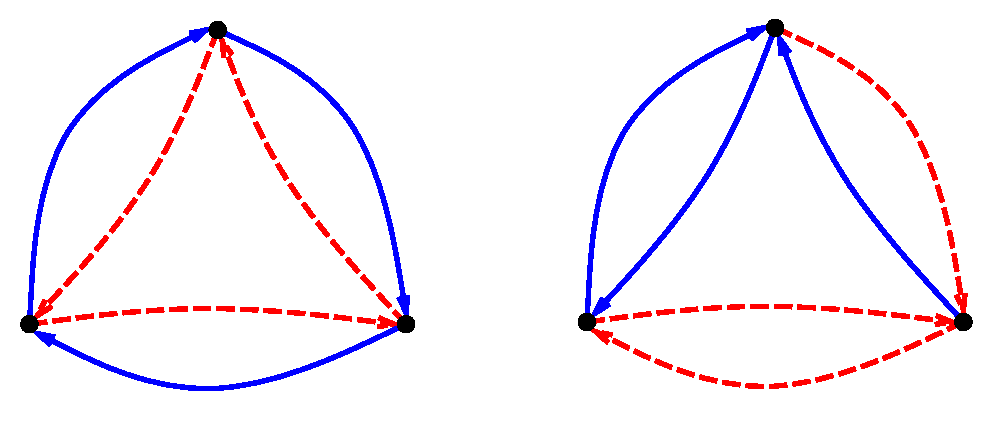
\includegraphics[scale=0.5]{Figs/UnsolvedPuzzles/roads}
\end{figure}

Гипотеза доказана для некоторых классов графов, например, если в каждый город заходят ровно две дороги, и число городов нечётно.%
\footnote{J. Friedman, ``On the Road Coloring Problem''. \emph{Proc A.M.S.}, Vol. 110, No. 4 (December 1990), 1133--1135}

[Со времени публикации английского оригинала этой книжки, эту задачу решил Абрам Трахтман.%
\footnote{A. N. Trahtman, 
``The road coloring problem''.
\emph{Israel J. Math.} 172 (2009), 51--60.}]


\subsubsection*{Круги в круге}

Эта прекрасная гипотеза сформулирована Александром Сойфером из Университета Колорадо.
Она и её родственницы стали предметом десятка статей в журнале Geocombinatorics, известно, например, что квадраты общей площадью 1 могут быть упакованы в квадрат общей площадью 2.
Обобщение на высшие размерности было предложено, в частности, вашим автором.
Случай двух шаров, каждый объёма $\tfrac12$, показывает, что $2^{d-1}$ нельзя улучшить.

\subsubsection*{Гипотеза Франкла}

Наша последняя головоломка о простейших математических объектах --- конечных множествах.
Увы, даже они способны привести в ступор.

Эта печально известная гипотеза, похоже, возникла впервые в 1970-х годах в творчестве Петера Франкла, венгерского математика, живущего в Японии (и являющегося там известной телевизионной фигурой).
С тех пор, она сводит комбинаториков с ума. 
На сегодня им даже не известно, существует ли элемент покрытый какой либо фиксированной долей множеств из семейства.

Очень хитрое доказательство Э. Кнолла, приведённое в статье Петра Вуйчика,%
\footnote{P. W\'{o}jcik, ``Union-Closed Families of Sets''. \emph{Discrete Math.}, Vol. 199 (1999), 173--182.}
показывает, что существует элемент, содержащийся по крайней мере в $N/\log_2 N$ множествах, где $N$ --- размер семейства.

Последний прогресс по головоломке был сделан Дэвидом Реймером из колледжа Нью-Джерси.%
\footnote{D. Reimer, ``An average set size theorem''. \emph{Combinatorics, Probability and Computing.} Vol. 12 (2003), 89--93.}
Реймер показал, что средний размер множества в семействе, замкнутом по объединению составляет по меньшей мере $\tfrac12\log_2N$ (это было недоказанное следствие гипотезы Франкла).

Многие простые вопросы о семействах множеств остаются открытыми.
Другой такой вопрос был предложен Вацлавом Хваталом из Рутгерского университета в 1972 году.
Предположим, что семейство $T$ множеств замкнуто относительно перехода к подмножеству, то есть любое подмножество множества в $T$ также содержится в $T$.
Предположим, мы нашли самое большое возможное пересекающееся подсемейство, то есть такое, что в любые два множества в нём имеют непустое пересечение.
Один из способов получения пересекающегося семейства состоит в том, чтобы взять все множества в $T$, содержащие фиксированный правильно выбранный элемент.
Гипотеза Хватала состоит в том, что лучше сделать невозможно.



\printindex


\newpage
{\sloppy
\tableofcontents

}

\end{document}
%ссылки  на источник даются в разном формате, я бы его униформуизировал 
%проверь разбивку на абзацы, иногда она у тебя не та, что у винклера 
%вы или Вы везде одинакого
%\heart после формул
%т.е. --> т.~е. --> то есть
%т. н. --> т.~н. --> так называемый
%кавычки «», ", выделения...
%,и; а также пробелы в мат. формулах
%.,; в формулах
%мы можем, вы можете --> можно
%мёртвые ссылки???
%унифицировать названия журналов
%\le\ge
%спросить ещё задач
%не хочет ли он что-то сказать русским читателям
%А́а́, Е́е́, И́и́, О́о́, У́у́, Ы́ы́, Э́э́, Ю́ю́, Я́я́
%тогда/то
